\documentclass{report}

\usepackage[a4paper,left=2.54cm,right=2.54cm, top=2.54cm, bottom=2.54cm]{geometry}	% better margins
\usepackage{booktabs} 			% tables with nice formatting
\usepackage{tabularx}			% tables with proper width
\usepackage{multirow}			% multi-row cells in table
\usepackage{gensymb}			% symbols
\usepackage[british]{babel}		% sets language formatting to British
\usepackage{csquotes}			% quoting commands
\usepackage[table]{xcolor}		% font colouring / table cell colouring
\usepackage{epigraph}			% epigraphs in chapters
\usepackage{parskip}			% better paragraph formatting
\usepackage{graphicx}			% image package
\usepackage{longtable} 			% To display tables on several pages
\usepackage{pgfgantt}			% Gantt Charts
\usepackage{pgfplots}			% draw charts and graphs
\usepackage{titlesec}			% used in chapter titles
\usepackage{subcaption}			% allows sub-figures
\usepackage{algorithm}			% algorithms
\usepackage{algpseudocode}		% algorithm formatting
\usepackage[fleqn]{amsmath}		% multiline math
\usepackage{amssymb}			% math symbols
\usepackage{xparse}				% adds string substitution for moveset command
\usepackage{courier}			% adds inline Courier font
\usepackage[binary-units]{siunitx}	% SI unit support
\usepackage{listings}			% code formatting
\usepackage[shortlabels]{enumitem}	% Lettered enumerations
\usepackage{tikz}				% flowcharts
\usepackage{mdframed}			% borders on aside environment
\usepackage[toc,page]{appendix}	% appendix package
\usepackage{pgfplotstable} 		% Generates table from .csv
\usepackage{textcomp}			% text symbols
\usepackage{etoolbox}			% allows custom environment pre/suffixes (listings -> minipage)
\usepackage[backend=bibtex,style=numeric-comp,sorting=none,sortcites=true,block=none,indexing=false,citereset=none,isbn=true,url=true,doi=true,natbib=true]{biblatex}
\usepackage{setspace}			% Line spacing
\usepackage{numprint}			% long number formatting
\usepackage[hidelinks]{hyperref}% linking throughout pdf

\setlength\bibitemsep{0.5\baselineskip}
\addbibresource{Dissertation.bib}

\sisetup{group-separator={,}}

\renewcommand{\epigraphsize}{\footnotesize}
\renewcommand{\textflush}{flushepinormal}

\usetikzlibrary{shapes.geometric, arrows, positioning}
\tikzstyle{startstop} = [rectangle, rounded corners, minimum width=3cm, minimum height=1cm,text centered, draw=black]
\tikzstyle{io} = [trapezium, trapezium left angle=70, trapezium right angle=110, minimum width=3cm, minimum height=1cm, text centered, draw=black, text width=3cm]
\tikzstyle{decision} = [diamond, minimum width=3cm, minimum height=1cm, text centered, draw=black, text width=2cm]
\tikzstyle{arrow} = [thick,->,>=stealth]
\tikzstyle{line} = [thick,-,>=stealth]
\tikzstyle{process} = [rectangle, minimum width=3cm, minimum height=1cm, text centered, text width=3cm, draw=black]

\titleformat{\chapter}{\normalfont\Huge\bfseries}{\thechapter}{1em}{}
\titlespacing*{\chapter}{0pt}{3.5ex plus 1ex minus .2ex}{2.3ex plus .2ex}

\definecolor{yellow}{HTML}{e5d600}
\definecolor{green}{HTML}{007f00}
\definecolor{keyword}{HTML}{bc4331}

\usepgfplotslibrary{dateplot}
\pgfplotsset{compat=1.8}

\BeforeBeginEnvironment{lstlisting}{\par\noindent\begin{minipage}{\linewidth}}
\AfterEndEnvironment{lstlisting}{\end{minipage}\par\addvspace{\topskip}}

\lstset{ 
	basicstyle=\small\ttfamily,
	captionpos=b,
	commentstyle=\color{gray},
	escapechar={|},
	frame=single,
	keepspaces=true,
	keywordstyle=\color{keyword},
	language=Python,
	morekeywords={half_turn_lookup, },
	stringstyle=\color{green},
	tabsize=4
}

\newcolumntype{M}[1]{>{\centering\arraybackslash}m{#1}}
\newcommand{\tbo}[1]{\textbf{#1}}
\newcommand{\tit}[1]{\textit{#1}}
\newcommand{\tun}[1]{\underline{#1}}
\newcommand{\propernoun}[1]{\enquote{\tit{#1}}}
\newcommand{\legopiece}[1]{(\##1)}
\newcommand{\moveset}[1]{\uppercase{\texttt{\{\formatmoves{#1}\}}}}
\newcommand{\movesequence}[1]{\uppercase{\texttt{:\formatmoves{#1}:}}}
\newcommand{\movegroup}[1]{\uppercase{\texttt{\formatmoves{#1}}}}
\newcommand{\face}[1]{\uppercase{\texttt{\formatmovesnospace{#1}}}-face}
\newcommand{\move}[1]{\uppercase{\texttt{\formatmovesnospace{#1}}}-move}
\newcommand{\colour}[1]{\uppercase{\tit{\texttt{\formatmoves{#1}}}}}
\newcommand{\slice}[1]{\uppercase{\texttt{\formatmovesnospace{#1}}}-slice}
\newcommand{\depth}[1]{depth-#1}
\newcommand{\uscore}{\texttt{\char`_}}
\newcommand{\legoindeximage}[1]{\includegraphics[width=0.2\textwidth]{Resources/Images/rdrLego#1.png}}
\newcommand{\customcenter}[1]{\multicolumn{1}{c}{#1}}
\newcommand{\lego}{LEGO }

\newcommand{\fw}{\color{gray}W }
\newcommand{\fo}{\color{orange}O }
\newcommand{\fg}{\color{green}G }
\newcommand{\fr}{\color{red}R }
\newcommand{\fb}{\color{blue}B }
\newcommand{\fy}{\color{yellow}Y }

\ExplSyntaxOn
\NewDocumentCommand{\formatmoves}{m}
{
	\tl_set:Nn \l__maxd_argument_tl { #1 }
	\tl_replace_all:Nnn \l__maxd_argument_tl {'} {'\;}
	\tl_replace_all:Nnn \l__maxd_argument_tl {@} {'}
	\tl_replace_all:Nnn \l__maxd_argument_tl {.} {\;\;}
	\tl_replace_all:Nnn \l__maxd_argument_tl {~} {\;}
	\tl_replace_all:Nnn \l__maxd_argument_tl {2} {\textsuperscript{2}\;}
	\tl_replace_all:Nnn \l__maxd_argument_tl {"} {\textsuperscript{2}}
	\tl_use:N \l__maxd_argument_tl
}

\NewDocumentCommand{\formatmovesnospace}{m}
{
	\tl_set:Nn \l__maxd_argument_tl {#1}
	\tl_replace_all:Nnn \l__maxd_argument_tl {'} {'}
	\tl_replace_all:Nnn \l__maxd_argument_tl {.} {\;}
	\tl_replace_all:Nnn \l__maxd_argument_tl {~} {\;}
	\tl_replace_all:Nnn \l__maxd_argument_tl {2} {\textsuperscript{2}}
	\tl_use:N \l__maxd_argument_tl
}

\tl_new:N \l__maxd_argument_tl
\ExplSyntaxOff

\newenvironment{aside}{\begin{mdframed}[style=0,%
		leftline=false,rightline=false,leftmargin=2em,rightmargin=2em,%
		innerleftmargin=0pt,innerrightmargin=0pt,linewidth=0.75pt,%
		skipabove=7pt,skipbelow=7pt]\small}
	{\end{mdframed}}

\pgfkeysifdefined{/pgfplots/table/output empty row/.@cmd}{
	\pgfplotstableset{
		empty header/.style={
			every head row/.style={output empty row},
		}
	}
}{}

\begin{document}
	\pagenumbering{gobble}
	\begin{titlepage}
	{\setstretch{1.5}
		
	    \centering
	   	\topskip0pt
	   	\vspace*{\fill}
	   	
		\includegraphics[width=0.6\textwidth]{Resources/Images/imgTUosLogo.png} \\
	   	\vspace{1.5cm}
	    {\Huge Analysis of Rubik's Cube Solution Algorithms with a Lego Mindstorms Robot} 
	    
		\vspace{1.5cm}
	    
	    {\huge Will Garside}
	    \vspace{2cm}
	    
	    {\Large Supervisor: Dr. Siobh\'{a}n North} \\
	    {\Large Department of Computer Science} \\
	    {\Large COM3610} \\
	    {\Large 2nd May 2018} 
	    
	    \vspace{0.8cm}
	    
		{\Large This report is submitted in partial fulfilment of the requirement for the degree of BSc Computer Science} \\
		{\Large \tit{by}} \\
		{\Large William O. R. Garside} \\
	
	    \vspace*{\fill}
	}
\end{titlepage}
	\newpage
	
	\renewcommand{\thechapter}{\Roman{chapter}}
	\pagenumbering{roman}
	\chapter{Declaration}
	All sentences or passages quoted in this report from other people's work have been specifically acknowledged by clear cross-referencing to author, work and page(s). Any illustrations which are not the work of the author of this report have been used with the explicit permission of the originator and are specifically acknowledged. I understand that failure to do this amounts to plagiarism and will be considered grounds for failure in this project and the degree examination as a whole.
	
	Name: William Garside\\
	Date: 02/05/2018

	\newpage
	\chapter{Abstract}
	Mathematicians and enigmatologists alike have been infatuated with Rubik's Cube for the past four decades, with countless algorithms and methods devised to solve it. Whilst the self-named \enquote{Cubers} have been playing with brightly coloured Cubes, \lego enthusiasts have been playing with small plastic bricks which have even more combinations than the Cube's forty-three quintillion. This project will combine these two groups with the aim of solving Rubik's Cube with a \lego Mindstorms robot and attempt to optimise the solution as far as possible. Various methods will be analysed and compared throughout the duration of the project, alongside the documentation of the robot building process. This is an entertaining and exciting  project, but complex algorithms will be picked apart and demonstrated through the \lego robot, with the final goal of pushing both the algorithms and the \lego Mindstorms to their limits.
	
	\newpage
	\chapter{Acknowledgements}
	I would like to express my thanks to Dr. Siobh\'{a}n North for suggesting this project and supervising my progress throughout. Thanks must also go to Rik van Grol, who provided invaluable information for one of the main algorithms used in this project.
	
	\newpage
	\chapter{Notation and Definitions}
	
	\section*{Singmaster Notation}
	
	The notation used in this document follows Singmaster Notation standards. For the following, \enquote{clockwise} denotes a rotation of that face when it is \tit{towards} the user. The addition of a \movegroup{@} symbol or a \movegroup{"} denote a counter-clockwise quarter rotation or half turn, respectively.
	
	\begin{enumerate}
		\item[] \movegroup{u} - rotates the \face{u} clockwise by \ang{90}
		\item[] \movegroup{d} - rotates the \face{d} clockwise by \ang{90}
		\item[] \movegroup{l} - rotates the \face{l} clockwise by \ang{90}
		\item[] \movegroup{r} - rotates the \face{r} clockwise by \ang{90}
		\item[] \movegroup{f} - rotates the \face{f} clockwise by \ang{90}
		\item[] \movegroup{b} - rotates the \face{b} clockwise by \ang{90}
	\end{enumerate}
	
	\section*{Basic Definitions}
	\begin{table}[H]
		\def\arraystretch{1.25}
		\centering
		\caption{Terminology used in this document}
		\label{tab:abbrev}
		\begin{tabular}{m{0.25\textwidth}m{0.65\textwidth}}
			\toprule
			\tbo{Abbreviation/Word} & \tbo{Definition} \\
			\midrule
			{[Rubik's]} Cube 	& 	A standard 3$\times$3$\times$3  Rubik's Cube. \\
			Face 				& 	One of the size faces on a Cube. Denoted by position or colour, e.g. \face{u}.\\
			Slice				&	A central layer between two faces. Usually referenced by the faces it spans. \\
			Quarter Turn		&	A clockwise rotation of a face or slice by \ang{90}. \\
			Half Turn			&	A clockwise rotation of a face or slice by \ang{180}. \\
			Quarter Turn Metric	&	When counting moves, a Quarter Turn is counted as a single move and a half is two moves. \\
			Half Turn Metric	&	Quarter turns and half turns are both counted as single moves. This is the metric used throughout this document. \\
			Cubie				&	One of the twenty-six smaller cubes that make up a Cube. \\
			Facelet				&	One of the fifty-four coloured squares on the faces of the Cube. \\
			Solved/Goal State			&	All the cubies on a given face match the colour of the centre cubie, i.e. a solved Cube. \\
			Position			&	A Cube's state (scrambled or solved). \\
			
			Moveset				&	A set of moves, denoted with curly braces, e.g. \moveset{u.d'l"} \\
			\multirow{ 2}{*}{Move Sequence}		&	A series of moves \tit{performed consecutively}, enclosed by colons. \\
			&	e.g. \movesequence{f.d.f'd2l'b'u.l.d.r.u.l'f'u.l.u"}. \\
			Solve Sequence		&	A move sequence which leads to the goal state. \\
			Depth-$n$			&	A Cube which has been moved $n$ times away from the goal state. \\
			\bottomrule
		\end{tabular}
	\end{table}

	\newpage
	\pagenumbering{gobble}
	\tableofcontents
   	\listoffigures
	\listoftables

	\newpage
	\renewcommand{\thechapter}{\arabic{chapter}}
	\pagenumbering{arabic}
	\setcounter{chapter}{0}
	\chapter{Introduction}
	\epigraph{I decided it was time to go home, let us put the cubes back in order. And it was at that moment that I came face to face with the Big Challenge: What is the way home?}{Ern\"{o} Rubik \cite{Rubik1986}}
	
    \section{Background}

    In 1974, Ern\"{o} Rubik was struggling to create a cube with independently moving parts which remain together, regardless of how much they moved. His first attempts made use of elastic, which broke and rendered the cube unusable. Rubik persevered in his attempts to hold the parts (now called \enquote{cubies}) together - eventually concluding that the best way was to have the cubies hold themselves together. He called this design \propernoun{The Magic Cube}, and it would go on to be one of the world's best-selling puzzles \cite{Waxman2014}. It was later re-branded to \propernoun{Rubik's Cube} to increase its marketability \cite{IdealToyCompany1980}.
    
    In an unpublished manuscript \cite{Rubik1986}, Rubik described first randomising his new cube, 
    
    \blockquote{\tit{It was wonderful to see how, after only a few turns, the colors became mixed, apparently in random fashion. Like after a nice walk when you have seen many lovely sights you decide to go home, after a while I decided it was time to go home, let us put the cubes back in order. And it was at that moment that I came face to face with the Big Challenge: What is the way home?}}
    
    It took Rubik over a month to solve this first cube - he knew intuitively that there must be a method to solving the cube, but lacked the finer methodology \cite{RubiksCube2017}. Since Rubik devised the first method, hobbyists and mathematicians alike have been immersed in solving the Cube as quickly and efficiently as possible. Whilst many solutions are markedly successful when it comes to optimisation, others only better them in quirkiness or internet fame \cite{Chan2016}.
    
    There is one method which, despite having been proved mathematically, is still little more than speculation: God's Algorithm. The theory behind this algorithm states that an omniscient being would always make the most efficient moves and that they would be able to solve a Cube from any given position in a certain number of moves or less. This is referred to as God's Number, and was finally proved to be twenty in 2010 by a group of four researchers \cite{Rokicki2010}.
    
    \section{General Objectives}
    The primary objective of this project is to successfully implement an algorithm to solve a Cube with a \lego Mindstorms robot. The efficiency of this algorithm is initially non-imperative, but will ideally be improved over the project time-line. The most recent iteration of the Mindstorms line, the EV3 31313, will be used in the construction of the robot. This provides wireless connectivity via Bluetooth or WiFi (via USB dongle), three motors, a colour sensor, and a touch sensor amongst other peripherals. A custom operating system can also be installed on a microSD card to allow for greater expansion.
    
    Secondary objectives include implementing other algorithms from various sources, devising and refining original algorithms, and comparing the performance, efficiency and sequence-length of the algorithm. The robot will have to be of sound construction, with little-to-no room for error when manipulating the Cube.
    
    \section{Limitations and Constraints}
    The first problem which will be encountered will undoubtedly be during the design and build of the robot: the number of pieces supplied in the EV3 set is quite limited at only six-hundred-and-one pieces - approximately a quarter of which are only for aesthetics. The design will be supplemented by sets sourced externally, thus allowing a robot of sufficient quality to be built. Despite being of high quality and uniform across all sets, \lego is still fundamentally a toy - which will lead to errors with the precision of the robot \cite{Cook2017}.
    
    One of the larger issues that this project will encounter is the run-time of the program to find a solution. Many programs have been known to take upwards of three days to find a solve sequence - this project currently aims to find a solution in approximately fifteen minutes or less (an arbitrary number determined only by the attention span of the author). This will require extensive optimisation of search spaces and group theory through symmetrical elimination and set covering in order to reduce the necessary coverage of the search algorithm.
    
    Finding the optimal solve sequence for any given position has been deliberately omitted from the objectives of this project: there are over forty-three quintillion positions of a Cube, each requiring an extensive amount of time to find the optimal solution for. Based on current hardware capabilities and previous studies and research, an estimated timespan for finding all optimal solutions is in the order of millennia\footnote{This is an estimation based on data presented at cube20.org which states that finding optimal solutions takes roughly \numprint{11800} times as long as finding sequences of twenty moves or less \cite{Rokicki2010}}.
    
    \newpage
    \chapter{Literature Review}
    \epigraph{Please forgive me, but to give birth to a machine is wonderful progress. It's more convenient and it's quicker, and everything that's quicker means progress. Nature had no notion of the modern rate of work. From a technical point of view, the whole of childhood is quite pointless.}{Mr. Fabry, in Karel \v{C}apek's \propernoun{Rossum's Universal Robots} \cite{Capek1921}}
    
    \section{Robotics}
    The term robot was first brought to the collective consciousness of the general public by Karel \v{C}apek in 1921 in his play \propernoun{Rossum's Universal Robots} \cite{Capek1921}. It comes from the Czech for \enquote{forced labour} and was coined by \v{C}apek's brother, Josef, for a short story written some years earlier \cite{Etymonline2017}. One of the main discussions in the field of robotics has been about ethics and morality. This discussion was started in \v{C}apek's play, when a visiting scientist tries to destroy the robot-manufacturing business, in the hope of giving the robots a soul and making them happier. This plan goes awry when, as is the norm in fiction surrounding Artificial Intelligence (AI), the robots become sentient and start to overthrow the humans that created them. Twenty-one years later, the novelette \propernoun{Runaround} by Isaac Asimov was featured in the magazine \propernoun{Astounding Science-Fiction} \cite{Asimov1942}. It included his now-prominent Three Laws of Robotics, which were a turning point in the field of robotics and meta-ethics.
    
    The twentieth century generated many ideas about the future of robotics, such as \enquote{Kitchen units will be devised that will prepare \enquote{automeals}, heating water and converting it to coffee} alongside grandiose aspirations such as \enquote{An experimental fusion-power plant or two will already exist in 2014} \cite{Asimov1964}. Whilst some predictions have been fulfilled by the technology of the past two decades, others are still nowhere near completion and could be considered impossible for the next century. This is a clear demonstration that the field of Robotics has made vast improvements, but is still - in some respects - very much in its youth.
    
    In the same way as Robotics, AI has vast potential and we have only touched the tip of the iceberg. The most advanced commercial AI systems are intended to make people's lives easier through organisation and saving precious seconds in performing simple tasks. However, Google's Assistant \cite{Google2016}, Apple's Siri \cite{Apple2011}, and Amazon's Alexa \cite{Amazon2014} still fall short when it comes to the intelligence demonstrated in Asimov's book \propernoun{I, Robot}. We are still far from being unable to \enquote{differentiate between a robot and the very best of humans} \cite{Asimov1970}.
    
    \section{Robotics in Education}
    There has been a clear use of \enquote{edutainment} style teaching in one form or another for hundreds of years. One of the earliest known uses of edutainment is in \propernoun{Poor Richard's Almanack}, which was written by Benjamin Franklin and published annually between 1732 and 1758. Alongside all the usual information contained in an Almanac, Franklin (under the pseudonym \propernoun{Poor Richard}) included maths exercises, puzzles, and aphorisms \cite{Beato2015}, \cite{Franklin1732}. Walt Disney was another pioneer of edutainment in the time immediately before, during, and following the World Wars. His first piece of edutainment was a short film, \propernoun{Tommy Tucker's Tooth}, which was commissioned by a dental institute in 1922.
    
    In the past few decades, there has been a marked change in edutainment, in line with advances in technology. We have progressed from paper-based, so called \enquote{serious games} in the 1970s, to early-era video games such as the infamous \propernoun{Oregon Trail}; and then in the past decade electronic and robotic kits have made their way into classrooms \cite{Becker}.
    
    Robotics has been described as \enquote{the most effective way of motivating and supporting the study of many areas}, and has also been shown to aid the development of social and teamwork skills \cite{Johnson2003}. In the past decade or so, robots and electronic kits have been a common extra-curricular activity and are increasingly being used as teaching aids and for practical sessions in actual lessons.
    
	One of the leaders of modern edutainment is the \lego Mindstorms kit. It has undergone two major revisions since the launch of the first generation in 1998 (the RCX): in July 2006, the NXT was released, updating the sensors and adding Bluetooth amongst other improvements; then in September 2013, \lego released the EV3 Home and Education sets. This release cemented \lego's position at the forefront of edutainment \cite{Becker}.
    
    \section{\lego Mindstorms}
    A study at the University of Calabria in 2009 looked at how \lego Mindstorms worked as a learning tool when used in team-building type tasks \cite{Bilotta2009}. Twenty-eight students were divided into six groups, each given a \lego robot and preliminary training which covered the Mindstorms and programming environment. The groups were all given the same task, and their progress studied throughout the sessions. When studying the building and programming as two distinct sub-tasks, three main categories of work subdivision were found, which closely follow real-world teamwork mechanics and scenarios. The use of robots was found to stimulate the students into exploring and sharing critical knowledge within the group. The study's conclusion was that \lego Mindstorms - and inherently other variable morphology robots - stimulate further process analysis, information selection, and experimentation and observations \cite{Bilotta2009}.
    
    The \lego Mindstorms' native programming environment is makes use of drag-and-drop code blocks to form software which can run natively on the main \enquote{control brick}. This provides a simplistic user experience and allows novice programmers to create complex pieces of software with relative ease. Drag-and-drop programming can drastically reduce the amount of syntax errors in a program, allowing programmers to better focus on functionality \cite{Kelleher2002}.

	\begin{figure}[H]
		\centering
		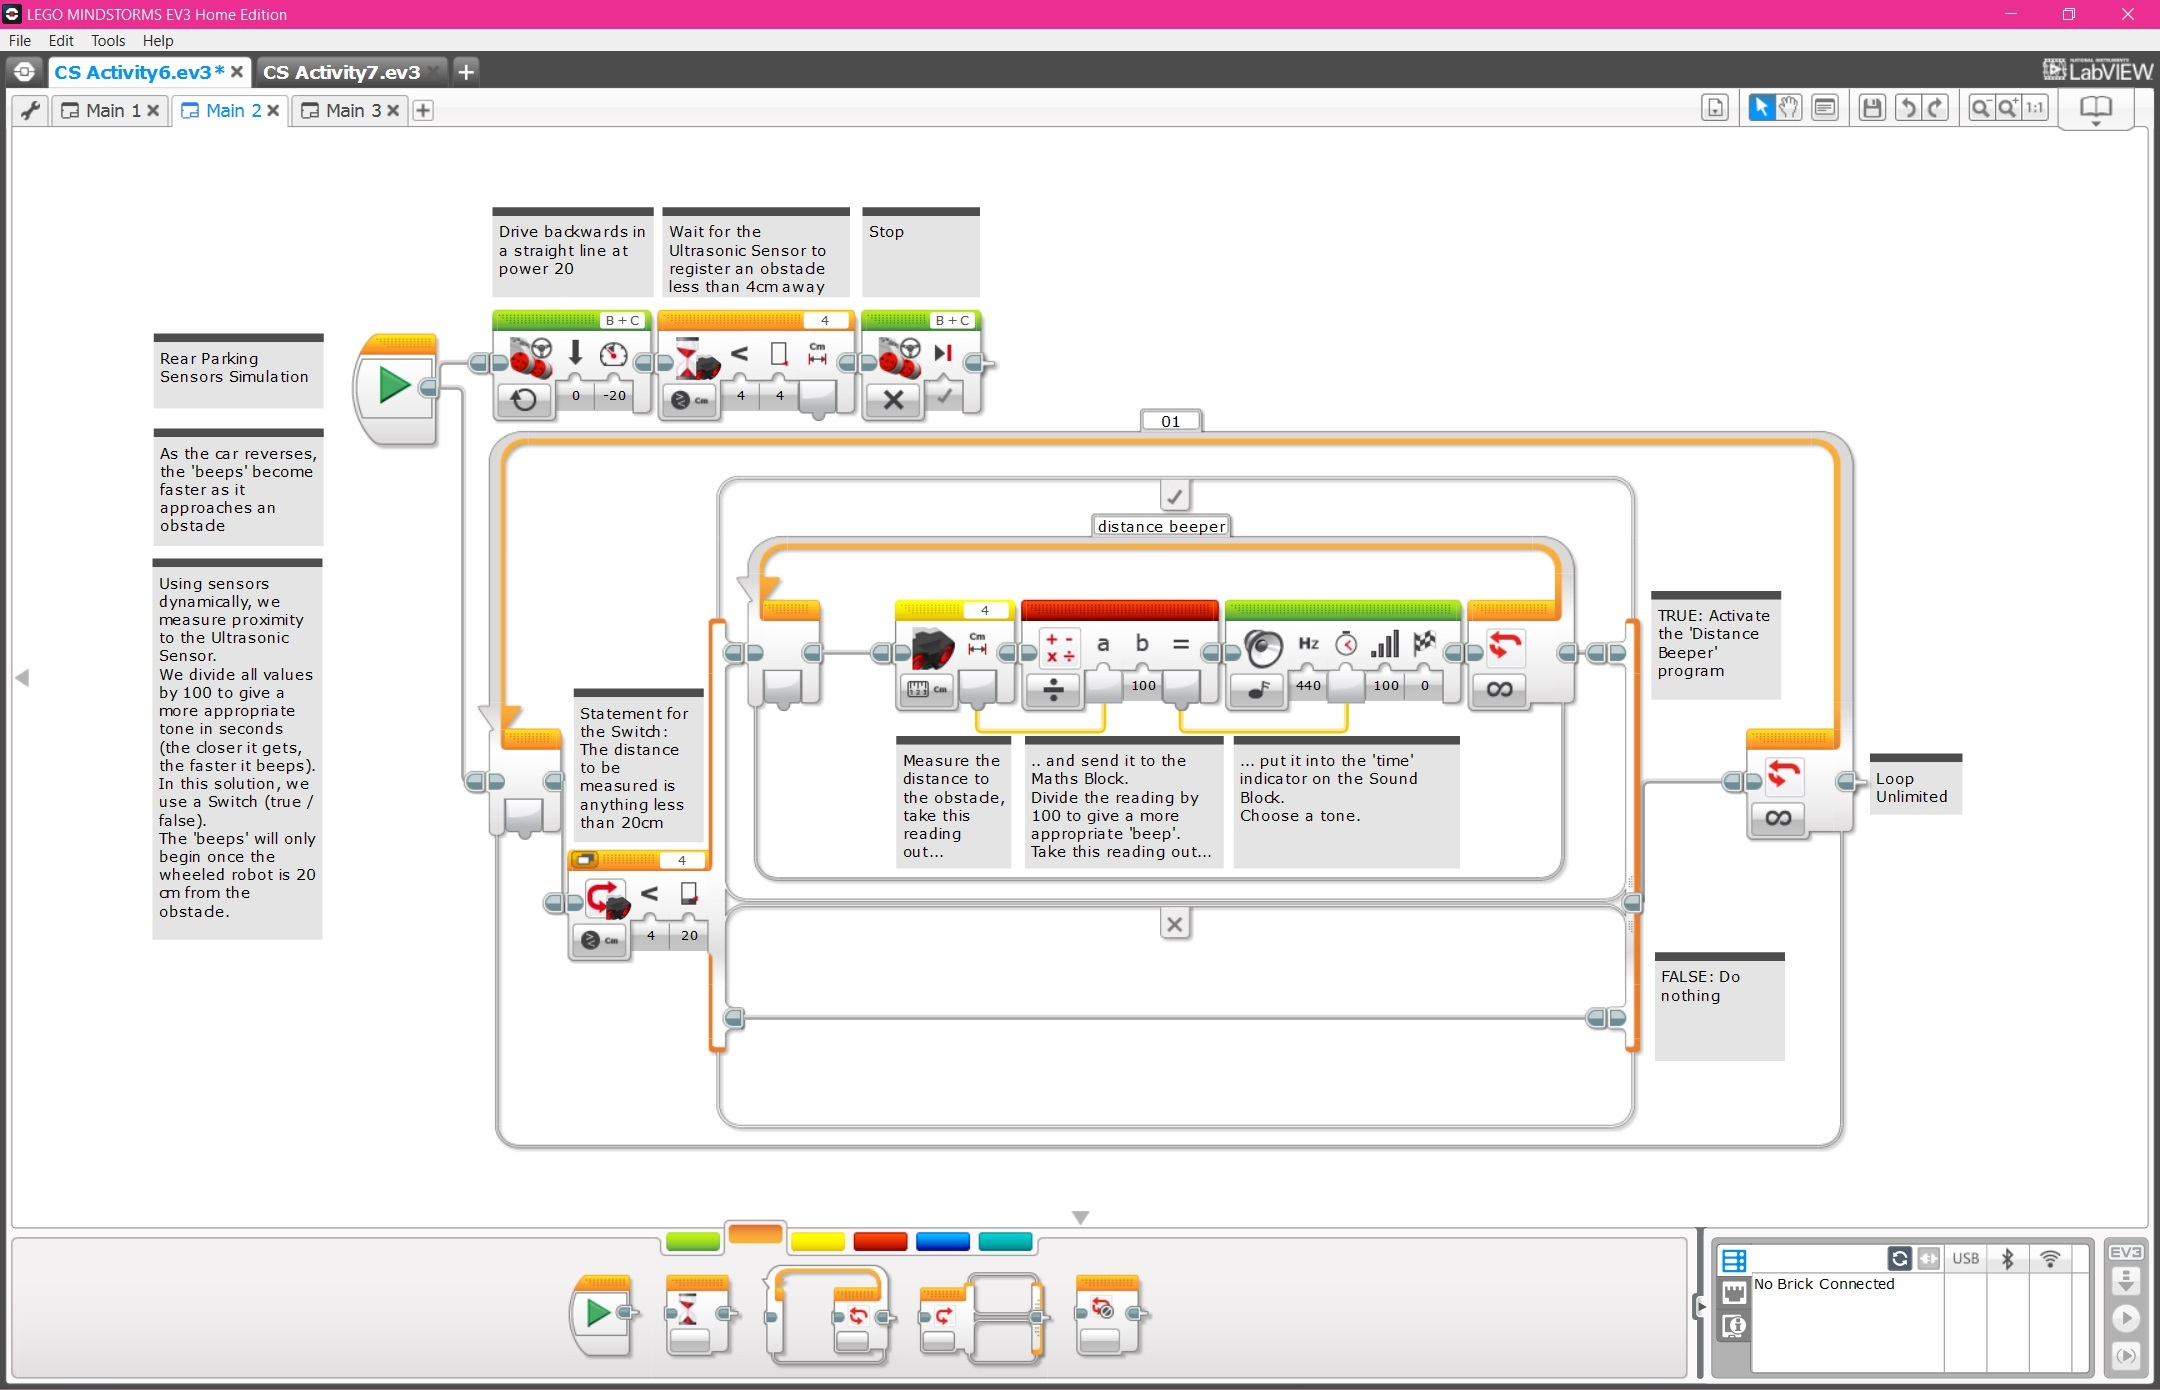
\includegraphics[width=0.5\textwidth]{Resources/Images/scrEV3ProgrammingSoftware.jpg}
		\caption{A sample program in \propernoun{EV3 Programming Software}}
		\label{fig:ev3software}
	\end{figure}
    
    \section{Solving Puzzles with Algorithms}
    When it comes to playing games and solving puzzles, Google's \propernoun{AlphaGo Zero} is the clear winner. Whilst Google's first Go-playing program did defeat the world champion at Go, it took months of supervised learning from experts and reinforcement learning from self-play. The new version started tabula rasa and was completely self-taught - it had no interaction with any humans, and used no historical data. Through reinforced learning alone by simulating games against itself, it took three days to reach the level of AlphaGo and in forty days had surpassed any Go player's performance - human or artificial \cite{Silver2017}, \cite{Cellan-Jones2017}.
    
    When a computer solves a Cube (or any other similar puzzle), it does so by following set algorithms and rules until the solved state is achieved. Computers cannot use humanlike instincts, so heuristics are often provided to make the task simpler. These heuristics can be pre-computed data tables to reduce the amount of processing at run time, or a reduction in the original data set by eliminating certain elements according to a set of rules.
    
    In his 1997 paper \cite{Korf1997} on the use of pattern databases to increase solve efficiency, Richard Korf uses different heuristic functions and characterises how effective they are in reducing the number of moves in a solve sequence. His first method used an Iterative-Deepening A* algorithm, combined with the heuristic of the Manhattan distances from the edge cubies' current position and orientation to the correct ones. This meant that the time required to solve a Cube at \depth{14} was about three days\footnote{The simulation was run on a Sun Ultra-Sparc Model 1 workstation}, however when increased to \depth{18} the time increased exponentially to two hundred and fifty years. After a re-evaluation, Korf modified the heuristic by pre-computing the Manhattan distance of each cubie from all of its possible positions and orientations and storing the table in memory at run-time. This created a table of nearly ninety-million entries - which would have been bigger but was restricted by the available memory (the table was approximately forty-two megabytes). The newer heuristic reduced the time to search at \depth{18} to less than four weeks - a reduction of approximately 99.97\%. Korf suggested that the speed of the algorithm used would increase linearly with the amount of memory available, meaning that if it were run today the \depth{18} search would take under three hours\footnote{This is based on the memory capacity of the Model 1 Workstation and a modern computer being 64 \si{\mega\byte} and 16 \si{\giga\byte} respectively.} \cite{Korf1997}.
    
    There have been many historical landmark algorithms since the inception of Rubik's Cube in 1974. One of the earliest instances was created by Morwen Thistlethwaite circa 1981 and is based on group theory. Thistlethwaite's algorithm splits all possible positions of the cube into five groups of decreasing size as seen in Table \ref{tab:thistlethwaite}. David Singmaster, Thistlethwaite's colleague, describes the methodology of the algorithm: \enquote{Once in $G_i$, one only uses moves in $G_i$ to get into $G_{i+1}$. The ratio $\frac{|G_i|}{|G_{i+1}|}$ is called the index of $G_{i+1}$ in $G_i$.} Using this algorithm, Thistlethwaite proved that the maximum number of moves required to solve any valid position is fifty-two \cite{Singmaster1981}. This was the first development of God's Number.
    
   	\begin{table}[H]
    	\def\arraystretch{1.25}
    	\centering
    	\caption{Morwen Thistlethwaite's five groups for his algorithm \cite{Singmaster1981}}
    	\label{tab:thistlethwaite}
    	\begin{tabular}{M{0.15\textwidth}M{0.3\textwidth}m{0.47\textwidth}}
    		\toprule
    		\tbo{Group Denotation} & \tbo{Mathematical Representation} & \customcenter{\tbo{Summary}} \\
    		\midrule
   			$G_0$	&	\moveset{l.r.f.b.u.d}	&	All valid positions \\	
	    	$G_1$	&	\moveset{l.r.f.b.u2d"}	&	All positions that can be reached with quarter turns of the \movegroup{l.r.f.b} faces and half turns of the \movegroup{u.d} faces \\
	    	$G_2$	&	\moveset{l.r.f2b2u2d"}	&	Positions reachable from quarter turns of \movegroup{l.r} faces and half turns of the \movegroup{f.b.u.d} faces \\
	    	$G_3$	&	\moveset{L2R2F2B2U2D"}	&	Positions only reachable from half turns of any face \\
	    	$G_4$	&	$ \{I\}$	&	The goal state \\
    		\bottomrule
    	\end{tabular}
    \end{table}
    
    \section{God's Number}
    The lower bound for God's Number was originally recognised to be eighteen moves through analysis of the number of sequences of seventeen moves or fewer, and the discovery that there were more Cube positions than seventeen-moves-or-fewer sequences \cite{Rokicki2010}. In 1995, the lower bound was increased to twenty by Michael Reid upon discovering that the \enquote{Superflip} position requires twenty moves to solve. He included his findings in an email to the \propernoun{Cube-Lovers} mailing list, \enquote{superflip is now known to require 20 face turns... this is the first improvement to the lower bound... given by a simple counting argument} \cite{Reid1995}.
    
    The next refinement to the upper bound of God's Number came from Dutch mathematician Hans Kloosterman in December of 1989. Kloosterman's findings were published in a newsletter \propernoun{Cubism for Fun} (CFF) as an article titled \propernoun{Rubik's Cube in 44 Moves}. In this article Kloosterman discusses his existing solution to the Magic Domino, a subset of Rubik's Cube, and how he has adapted it into a more efficient Cube solution with the help of Thistlethwaite's algorithm. Kloosterman reduced the estimation of God's Number by adapting Thistlethwaite's $G_3$ into a subgroup of $G_2$ where all of the $U$-cubies are on the $U$ face and all the $D$-cubies are similarly on the $D$ face. This reduces the index $\frac{|G_2|}{|G_3|}$ from 15 to 8 (whilst also reducing the ($G_1:G_2$) index by 3 and increasing the ($G_3:G_4$) index by 1), creating a net decrease of 8 moves when compared to Thistlethwaite's algorithm. \propernoun{Rubik's Cube in 44 Moves} ended with an editor's note stating that not all of the details of the algorithm were certain and more (including a more efficient algorithm) would be revealed in a later issue \cite{Kloosterman1989}.
    
    Sure enough, a year later Kloosterman wrote an article titled \propernoun{Rubik's Cube in 42 Moves} in the twenty-fifth issue of CFF. This stated that the new algorithm was in fact the final version of Kloosterman's forty-four move algorithm. In the same way as its predecessor, this article is split into four stages to solve a Cube. The first three stages are based on solving a Cube with only certain cubies coloured - the positions of the other remain irrelevant until a later stage. The final stage is solving the Cube in a non-particular manner, and is calculated to take no more than eighteen moves \cite{Kloosterman1990}.
    
    In the following twenty years, the upper bound was gradually refined to match the lower bound - God's Number is exactly twenty. The final development came from a group of four Rubik's Cube enthusiasts in July of 2010, and was only achieved through a brute force method: the four-man team first took every possible position of a Cube and reduced it from forty-three quintillion positions down to just over one quintillion - still a vast number, but a large reduction nevertheless - by using rules of symmetry and mirroring. They then wrote a program to find solve sequences of length twenty or less, which found all solve sequences in a few weeks \cite{Rokicki2010}.
    
   	\begin{figure}[H]
   		\centering
		\begin{tikzpicture}
			\begin{axis}[title={God's Number}, axis lines = left, date coordinates in=x, enlarge x limits=false, xticklabel={\year},	date ZERO=1980-01-01, xmin=1980-01-01, xmax=2020-01-01, xtick={1980-01-02,1990-01-01,2000-01-01,2010-01-01,2020-01-01}, ylabel = Sequence Length, xlabel=Year]
			\addplot coordinates {
				(1981-07-01, 52)
				(1990-12-01, 42)
				(1992-05-01, 39)
				(1992-05-01, 37)
				(1995-01-01, 29)
				(1995-01-01, 29)
				(2005-12-01, 28)
				(2006-04-01, 27)
				(2007-05-01, 26)
				(2008-03-01, 25)
				(2008-04-01, 23)
				(2008-08-01, 22)
				(2010-07-01, 20)
				(2018-01-01, 20)
			};
			\addplot coordinates {
				(1981-07-01, 18)
				(1990-12-01, 18)
				(1992-05-01, 18)
				(1992-05-01, 18)
				(1995-01-01, 18)
				(1995-01-01, 20)
				(2005-12-01, 20)
				(2006-04-01, 20)
				(2007-05-01, 20)
				(2008-03-01, 20)
				(2008-04-01, 20)
				(2008-08-01, 20)
				(2010-07-01, 20)
				(2018-01-01, 20)
			};
			\legend{Upper Bound, Lower Bound}
			\end{axis}
		\end{tikzpicture}
   		\caption{The upper bound was decreased to 20 over the course of twenty-nine years and across thirteen separate studies \cite{Rokicki2010}. Data attached in Appendix \ref{tab:godsNumber}}
		\label{fig:godsnumbergraph}
	\end{figure}

    
    \section{Python as a Scientific Scripting Language}
    Traditionally when performing large calculations and processes, compiled languages are the preferred choice over scripting languages. This is because compilation is done before run-time, allowing the program to run unhindered by on-the-fly translation/interpretation \cite{Cai2005}.
    
    For general purpose applications, scripting languages are preferable because they allow small changes to be made without re-compiling large classes before testing. In the thirteenth issue of \propernoun{Scientific Programming}, Cai, Langtangen and Moe \cite{Cai2005} explain how MATLAB is often a preferable choice for less intensive scientific computation due to its many features, such as integrated simulation and visualisation tools, clear syntax and immediate feedback of commands. They describe the use of MATLAB in computational science as paradoxical, as it is a scripting language rather than compiled.
    
    One of MATLAB's biggest selling points, the integrated development environment (IDE) with support for matrices, graphs and other mathematical features, can be replicated in a few Python IDEs or with the addition of Python packages. One of the most popular packages, \propernoun{Numerical Python} (NumPy), adds support for most scientific calculations. It expands Python's inbuilt data structures to use multi-dimensional homogeneous arrays of any Python data type. NumPy takes Python from a well-structured general-purpose language to a powerful mathematical language which can be applied to many different tasks \cite{Cai2005}, \cite{Oliphant2006}.
    
    As well as the multitude of available packages, Python has another major tool in its arsenal: it can be extended with a compiled language by design. This means that processor-intensive tasks can be migrated to a compiled language such as C++ or Fortran, increasing run speed up to a factor of ten. This extension process is now a trivial matter thanks to automated tools such as \propernoun{f2py}, which allows for automated calls to compiled Fortran code \cite{Oliphant2006}.
    
    \section{Conclusion}
    \lego Mindstorms is a strong choice for the construction of the robot: its variable morphology allows adaptation to a range of tasks; the uniformity between pieces means that the main EV3 kit can be supplemented with other kits to extend its ability; and previous studies have shown that it is ideal for stimulating analysis and observations. Instead of using a single algorithm to solve the Cube, a range will be implemented in order to find the strongest method for finding a solve sequence. This will allow cross-comparison between, and analysis of, individual algorithms with the intention of finding the algorithm best suited to this project. Tree and group based algorithms alike will be implemented.
    
    MATLAB is incompatible with the \lego EV3, so will not be used for this project. Python's wide compatibility, clear high-level syntax, and extendibility to compiled code for more complex calculations, makes it the ideal language for this project.
   
    \newpage
    \chapter{Requirements and Analysis}
    \epigraph{I have yet to see any problem, however complicated, which when you looked at in the right way, did not become still more complicated.}{Paul Anderson, for New Scientist \cite{Anderson1969}}
    
    \section{Introduction}
    
    This chapter covers the specific requirements needed for the project to succeed: the particular tasks to complete the project; the hardware required to build the robot and run the software; and the IDEs needed to write and run it. As well as the requirements, an in-depth analysis of the project and its goals is made, discussing their feasibility, difficulty, and how necessary they are for the success of this project.
    
    \section{Specific Aims and Objectives} \label{sec:objectives}
    
    \begin{enumerate}
    	\item Build a robot which can manipulate a Cube accurately \par This is the first of the two primary objectives for this project, and is imperative to the project's success. As such it will be the first objective to be completed. This task, despite being of a medium difficulty, is fairly straightforward by nature: the robot simply needs to manipulate a Cube in any valid move.
    	\item Implement a system which successfully generates a solve sequence for any given position. \par The second primary objective ensures that any of the forty-three quintillion positions of Rubik's Cube can be solved correctly. The time taken to generate the solve sequence and the actual length of the solve sequence will both be used when measuring an algorithm's success.
    	\item When the robot is provided with a move sequence, it should...
    	\begin{enumerate}
    		\item Convert it to be robot-compatible \par All of the pre-existing algorithms return a solution which a human being can follow to solve a real-world Cube. For this project the manipulation is done by the robot, which may not be able to perform all of the standard moves, so any sequences provided must be translated.
    		\item Correctly follow the sequence to achieve the intended output \par Once a robot-compatible move sequence has been generated, the robot must move the Cube in this exact sequence with no errors or move-failures. If a single move is performed incorrectly then the entire move sequence will produce an incorrect output.
    	\end{enumerate}
    	\item Ensure the runtime of the system is an acceptable length \par Previous algorithms have had a run-time in the order of weeks: the desired run-time of the generation by this project will be in the order of minutes. This will require careful analysis of the trade off between generator efficiency and solve sequence length.
    	\item Implement software which uses a range of algorithms to generate a solve sequence \par In order to effectively compare the performance of several algorithms, there must be a method of running them under the same conditions and with the same overheads (e.g. transmission time to the robot). For this reason, there will be one main program with an option for the algorithm to use.
    	\item Compare the performance of different algorithms, especially the difference between human and robot compatible move sequences \par The performance of each algorithm will be tracked and compared fairly to show each one's merits and faults. This will allow the choice of one algorithm to be improved to create the most efficient method - or the potential combination of algorithms to form a stronger one.
    \end{enumerate}
    
    \section{Analysis}
    \subsection{Software}
    
    \subsubsection{PyCharm}
    An IDE makes development, running programs, and testing and debugging much easier than using a simple text editor and command line. PyCharm by JetBrains \cite{JetBrains} will be used for developing in Python. PyCharm provides strong code completion abilities, project-wide refactoring, and software development kit (SDK) modification amongst many other abilities. This will allow more time to be allocated to tasks of higher value rather than struggling with relatively minor issues.
    
	\subsubsection{Python 3.6 Runtime Environment}
    Python requires a native runtime environment for programs to be run: this consists of the Python interpreter, libraries, and any packages used in the development process.
    
    \subsubsection{ev3dev}
    ev3dev \cite{Ev3dev.org} is a custom operating system (OS) for the EV3 which contains a low-level framework for the peripherals of an EV3. It allows users to write their own programs in a multitude of languages to create complex functions and models. It is installed by flashing the ev3dev OS to a microSD card which is then inserted into the EV3, avoiding affecting the EV3's original firmware.
    
    A Python wrapper is available on GitHub \cite{Ev3dev} for the ev3dev OS, allowing the creation of Python programs with packaged support for the actuators and sensors of the EV3.
    
    \subsection{Software Requirements}
    
    This table shows the requirements of the software to be used in the creation of this project. The specifications of the computer being used for the development of this project are listed in this table to show how the requirements are satisfied.
    
	\begin{table}[H]
		\small
		\def\arraystretch{1.5}
		\centering
		\caption{Software requirements for the main development computer and its capabilities}
		\label{tab:winSoftware}
		\begin{tabular}{M{0.2\textwidth}M{0.15\textwidth}M{0.15\textwidth}M{0.15\textwidth}M{0.15\textwidth}}
			\toprule
			\multirow{2}{*}{\tbo{Software}} & \multicolumn{4}{c}{\tbo{Requirements/Capabilities}} \\
			& Minimum OS & Processor & Memory & Connectivity \\
			\midrule
			PyCharm	&	Windows 2003	&		&	2GB	& \\
			\lego EV3 Programming Software\cite{Lego2017}	&	Windows 2003	&	Dual Core 2GHz	&	2GB	&	1 USB Port \\
			Python 3.6	&	Windows Vista	&	{\scriptsize Program Dependent}	&	{\scriptsize Program Dependent}	&	{\scriptsize Program Dependent} \\
			\midrule
			\tit{Main Development Computer}	&	\tit{Windows 10 Pro 64-bit}	&	\tit{Quad Core i5 6500 3.6GHz}	&	\tit{32GB}	&	\tit{WiFi, Bluetooth} \par \tit{12 USB Ports}\\
			\bottomrule
		\end{tabular}
	\end{table}

	\subsection{Cube Choice}
	
	The type of Cube to be used is a \propernoun{Valk 3}, which is a speedcube. This means that it has low turning resistance and is a good quality product so will not break under repeated testing conditions.
    
    \section{Feasibility Evaluation}
    \subsection{Optimal Solutions}
    
	The immense size of the Cube position search space means that finding the optimal solution for every position is an intractable problem. Research carried out by Rokicki et al. (2010) to definitively prove God's Number found a solution for every position with a length less-than-or-equal-to twenty. This research was carried out on \enquote{a large number of computers at Google}, and took the equivalent of thirty-five CPU years \cite{Rokicki2010}. The program they wrote could solve Cubes in twenty positions or less at a rate of 3600 positions \si{\per\second}, but when set to find optimal solutions the rate dropped to 0.36 positions \si{\per\second} - a reduction by a factor of $10^4$.
    
	\subsection{Tree Based Methods}
	
	Although the problem of finding all optimal solutions is likely infeasible within the scope of this project, a tree-based method will prove or disprove the hypothesis. It will also provide a greater understanding into the generation and navigation of a search space for Cube positions. A basic search tree will be very difficult to successfully solve any Cube, as it will grow exponentially at a rate of $d^6$. Optimisations and heuristics can be used to make the tree generation easier and more efficient, however they still may not make the problem manageable on account of its sheer scale.
	
    \subsection{Group Based Methods}
    
    A more tractable method for solving positions is the use of pre-defined groups with lookup tables, which was commonly used throughout the development of God's Number. The (self-imposed) constraint of solving a Cube in a reasonable time is removed through the use of lookup tables, because the positions are already generated. It is this table generation which will present an obstacle in solving a Cube. A significant portion of the forty-three quintillion positions will need to be generated and stored in a database for a comprehensive lookup.
    
    The definition of the groups and their effectiveness will have to be tested and analysed, along with their combined functionality. Extensive research into different group types and combinations could be used to reduce the magnitude of the problem at hand - although this may be limited by the imposed time-scale.
    
    \section{Evaluative Techniques} \label{sec:evalTechniques}
    
    This project is of quite a closed nature, in that there is very little commercial value and inherent user testing. Instead, all evaluation of this project will be internal and ultimately quantifiable into categories such as \enquote{Cube Solved}, \enquote{Efficient Solve}, and \enquote{Quick Solution Generation}. The quickest way of measuring the success of this project is whether or not any position can be successfully solved in a relatively short amount of time (e.g. $<10$ \si{\minute}). 
    
    The main objectives for this project have been defined in Section \ref{sec:objectives} and the project will aim to meet them throughout. In Chapter \ref{chp:resultsDiscussion} the completed implementation of the project will be measured against the objectives.
    
    The progress of this project is estimated to follow the below Gantt Chart. For the duration of its lifespan, there will be a continual measurement of the actual progress against predicted.
    
    \begin{figure}[H]
		\begin{ganttchart}[title/.append style={fill=black!10}, hgrid, x unit=0.4mm, y unit title=7.5mm,, y unit chart=5mm, vgrid={*{6}{draw=none},dotted},	milestone/.append style={xscale=10}, time slot format=isodate]{2017-07-03}{2018-04-29}
			\gantttitlecalendar{year, month=shortname} \\
			\ganttgroup{\small Robot}{2017-07-15}{2017-09-18} \\
			\ganttbar{\small Design}{2017-07-20}{2017-08-20} \\
			\ganttbar{\small Build}{2017-08-08}{2017-09-04} \\
			\ganttbar{\small Testing}{2017-09-01}{2017-09-15} \\
			\ganttbar{\small Refinement}{2017-09-05}{2017-09-17} \\
			\ganttmilestone{\small Complete}{2017-09-18} \\
			\ganttgroup{\small Codebase}{2018-02-01}{2018-04-15} \\
			\ganttbar{\small Binary Search Method}{2018-02-05}{2018-02-25} \\
			\ganttbar{\small Primary Solve Method}{2018-02-24}{2018-03-05} \\
			\ganttmilestone{\small Cube Solved}{2018-03-05} \\
			\ganttbar{\small Primary Refinements}{2018-03-05}{2018-03-12} \\
			\ganttbar{\small Further Algorithms}{2018-03-10}{2018-03-20} \\
			\ganttbar{\small Performance Comparison}{2018-03-20}{2018-03-31} \\
			\ganttmilestone{\small Optimal Solve}{2018-04-05} \\
			\ganttbar{\small Implementation}{2018-03-16}{2018-04-04} \\
			\ganttbar{\small Testing}{2018-03-30}{2018-04-05} \\
			\ganttgroup{\small Final Write Up}{2017-09-20}{2018-04-29} \\
			\ganttbar{\small Introduction}{2017-09-23}{2017-10-02} \\
			\ganttbar{\small Research}{2017-09-28}{2017-12-12} \\
			\ganttbar{\small Literature Review}{2017-10-03}{2017-11-13} \\
			\ganttbar{\small Requirement Analysis}{2017-10-28}{2017-11-20} \\
			\ganttbar{\small Results and Discussion}{2018-03-24}{2018-04-17} \\
			\ganttmilestone{\small Conclusions}{2018-04-20} \\
		\end{ganttchart}
		\caption{The estimated progress of this project during its timeline}
	\end{figure}

 	\vskip\baselineskip
 	\vskip\baselineskip
 	
    \begin{aside}
    	The large gap in the Gantt chart between the completion of the robot and the beginning of the codebase development is due to other work commitments and priorities. This has been shown in the Gantt chart to maintain a realistic presentation of this project and its progress throughout. During this time away from core development, progress will be made on this document.
    \end{aside}
    
    \newpage
    
    \chapter[Design, Implementation and Testing: The Robot]{Design, Implementation \\ and Testing: The Robot} \label{chp:designRobot}
    \epigraph{I don't spend my time pontificating about high-concept things. I spend my time solving engineering and manufacturing problems.}{Elon Musk \cite{Ohnsman2013}}
    
	\section{Introduction}
	
	The nature of this project lends itself to a spiral design cycle, where both the robot and the solver can be designed, implemented, tested and then optimised to re-start the cycle. This non-linearity of the \tit{Design $\rightarrow$ Implementation $\rightarrow$ Testing} process means that the structure of this document must follow the progress of the project, rather than having distinct sections for \enquote{Design} and \enquote{Implementation and Testing}. Consequentially this part is split into two chapters - \enquote{Robot} and \enquote{Codebase} - each with introductory sections for fundamental components that are invariant through the different iterations, and further sections to discuss each iteration individually.
	
	Special semantics are used in this chapter to denote move sequences and sets. A glossary is available on page \pageref{tab:abbrev}.

	\begin{figure}[H]
		\centering
		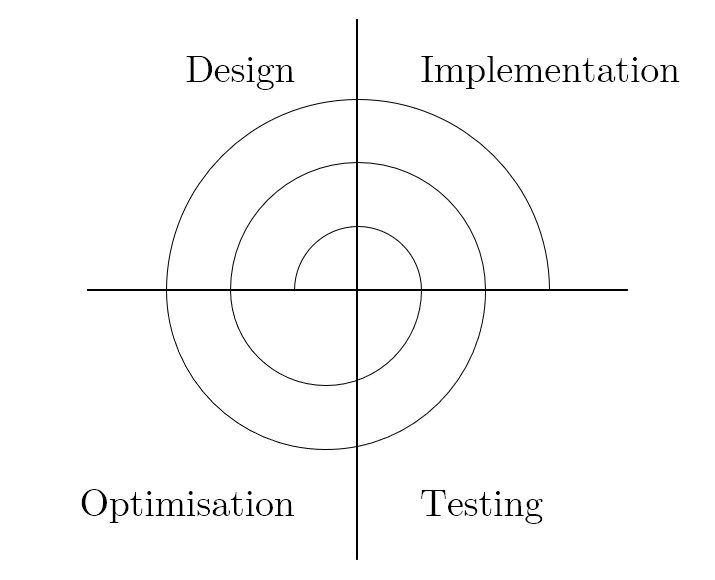
\includegraphics[width=0.3\textwidth]{Resources/Images/diagSpiralModel.png}
		\caption{The spiral model used for this project}
		\label{fig:diagSpiralModel}
	\end{figure}

    \section{Robot Fundamentals and Prototyping}
    
    \subsection{Sensors and Actuators}
    
    The \lego EV3 is provided with three DC motors (two large \legopiece{45502}\footnote{Specific mentions of \lego pieces are indexed in Appendix \ref{tab:legoIndex}} and one medium \legopiece{45503}), a colour sensor \legopiece{45506} and a touch sensor \legopiece{45507} amongst other peripherals\footnote{The other peripherals are an infrared sensor and an infrared beacon, and are not used in this project.}. The quantity of the motors will be the largest restriction in designing the robot: it will only be able to rotate a Cube about two of the three axes; and the colour sensor will only have one degree of freedom so will rely on the rotation of the Cube to scan all of the facelets. The touch sensor can be used to allow limited user input to the robot at runtime, such as an emergency stop if the Cube becomes dislodged, or to confirm that the Cube is in place.
    
    \subsection{Prototyping with \lego}
    
    The first step in designing the robot was to prototype some simple designs for holding a Cube and successfully manipulating it. The first concept design gripped each face of the Cube, and use a large motor to power the \enquote{grippers}. The second large motor would control which gripper was being powered at any time. This would allow a strong manipulation of the Cube and mean no delay between the movement of different faces. Figure \ref{fig:imgPrototype} shows the initial prototype that was built to fit this design. This would be difficult to implement because if one of the grippers rotated by a quarter turn, it would block two of the other faces from turning. This can been seen below, where the upper gripper is blocking the left-hand one from turning. The solution to this would be to have the grippers retract when they are not in use, however this would be very difficult - if not impossible - to achieve with the available \lego pieces.
    
    \begin{figure}[H]
		\centering
		\begin{subfigure}[b]{0.30675\textwidth}
			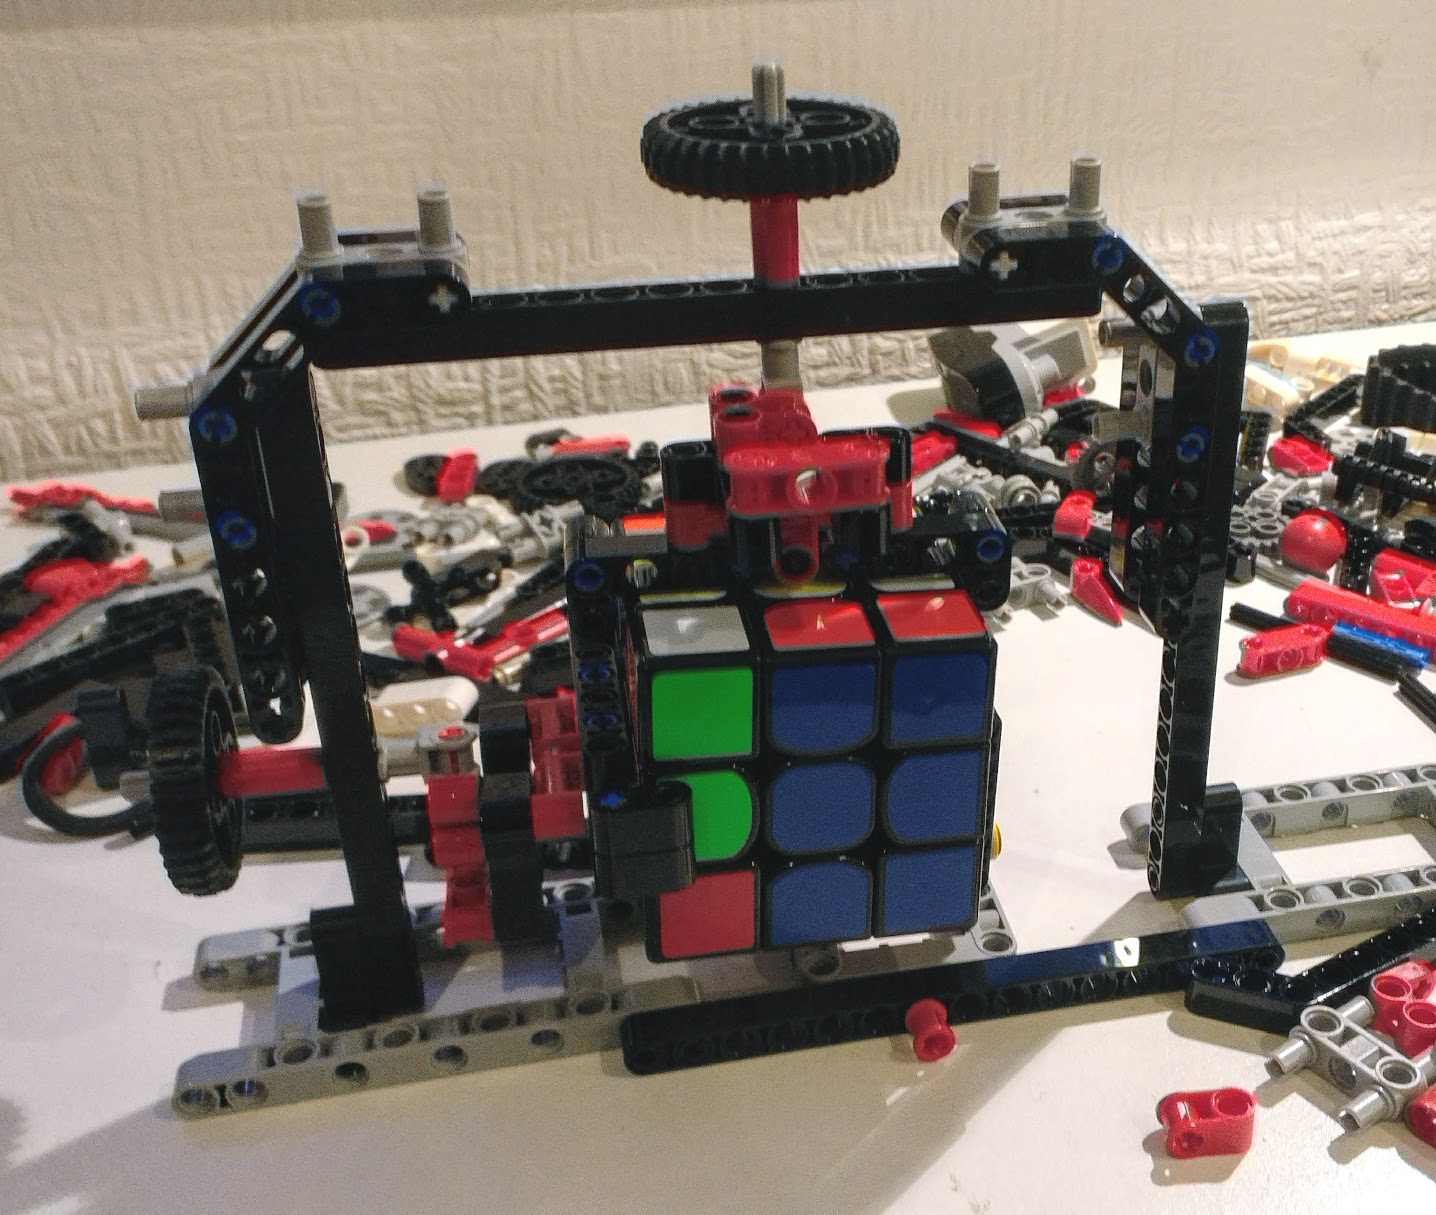
\includegraphics[width=\textwidth]{Resources/Images/imgPrototype.jpg}
			\caption{The first prototype}
			\label{fig:imgPrototype}
		\end{subfigure}
		\hspace{10mm}
		\begin{subfigure}[b]{0.44325\textwidth}
			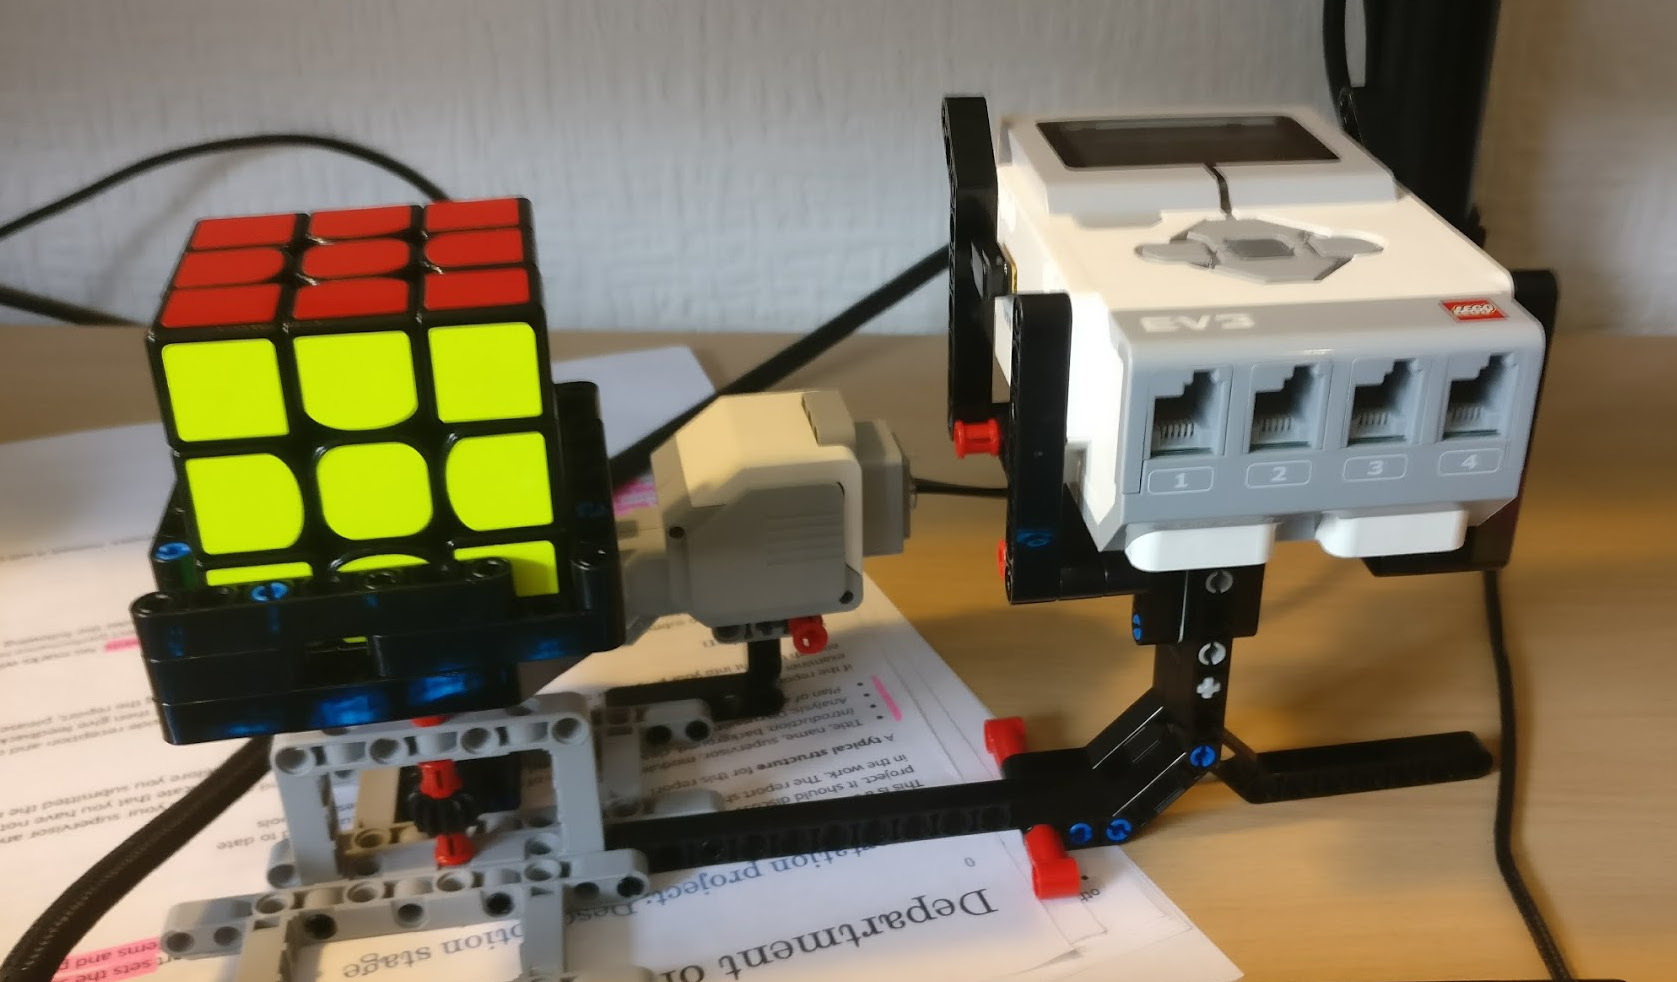
\includegraphics[width=\textwidth]{Resources/Images/imgCradleTest.jpg}
			\caption{The model used to test the motor's torque}
			\label{fig:imgCradleTest}
		\end{subfigure}
		\caption{A cross-section of the cradle and Cube}
		\label{fig:imgPrototypes}
	\end{figure}

	One of the other problems with the first prototype was that the Cube was unbalanced and would often fall out of the robot. This led to the design to have a \enquote{cradle} for the Cube to sit in. This is a good support mechanism for the Cube, and also provide the rotation about the Y axis. Once the cradle was built, it was a good milestone to check that the large motors had enough torque to rotate the face of a Cube against the friction between faces and slices. The motor was set to rotate indefinitely with the Cube in the cradle (as seen in Figure \ref{fig:imgCradleTest}) and the \slice{l-r} manually held in place. There was no visible reduction in the rotational velocity of the motor, so this first small test was passed.
	
	Although the cradle was a good solution to the problem outlined above, it also meant that only the \face{d} could be rotated, therefore requiring a mechanism to \enquote{flip} the Cube in place so different faces could sit in the cradle. The most obvious design for this was to apply a force at the upper corner to create a resultant force to pivot about the wall of the cradle, as shown by the free body diagram in Figure \ref{fig:dwgCubeFreeBodyDiagram}. Once the Cube is pushed out of the cradle, it will slide back into place due to the height difference between the wall and the base of the cradle, and the low coefficient of friction between the plastic of the Cube and the \lego pieces.
    
	\begin{figure}[H]
    	\centering
   		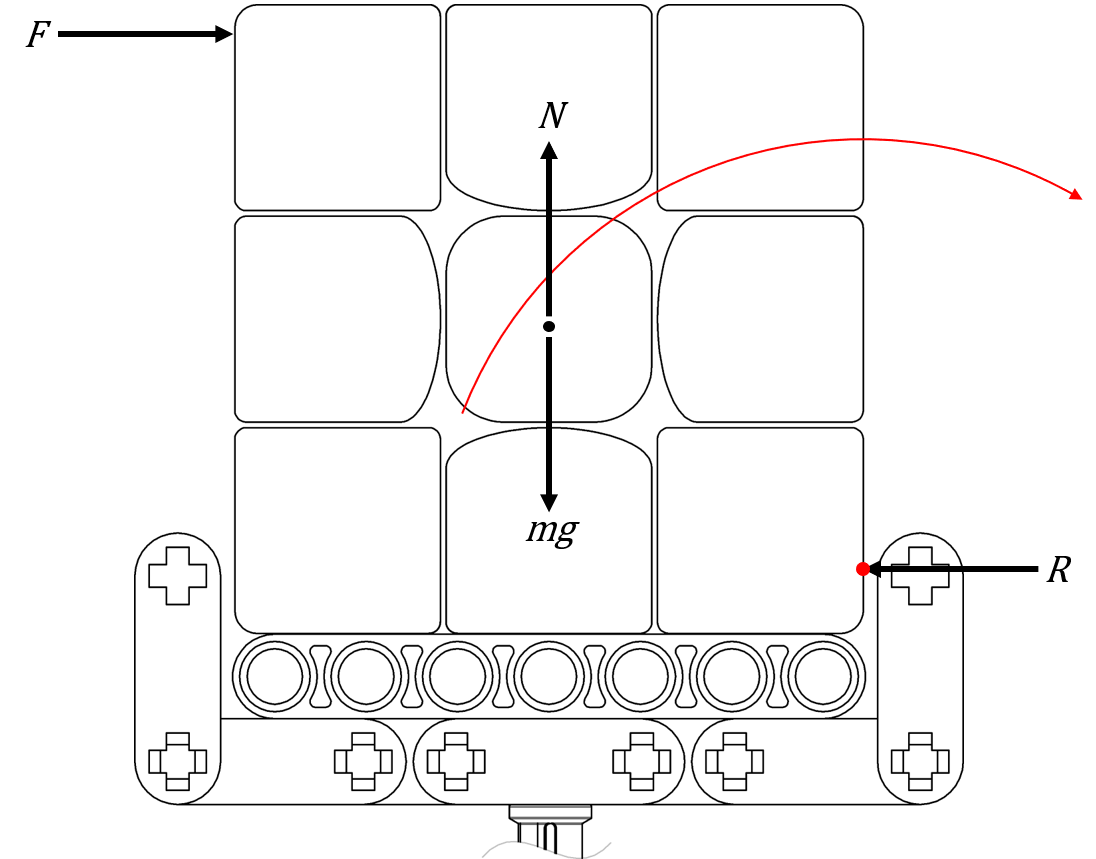
\includegraphics[width=0.35\textwidth]{Resources/Images/dwgCubeFreeBodyDiagram.png}
   		\caption{A free body diagram showing how the Cube will be rotated}
   		\label{fig:dwgCubeFreeBodyDiagram}
    \end{figure}
    
    \subsection{Fundamental Component Definitions} \label{sec:componentDefinitions}
    
    Following the construction and analysis of small \lego prototypes, it became apparent that there would be three fundamental components for the archetypal robot: a cradle would be needed to hold the Cube and rotate about the Y axis; an arm to rotate the Cube about the X axis and hold it in place for performing \move{d}s; and a moving arm for the colour sensor to scan the Cube.
    
    \subsubsection{Cradle}
    
    The Cube will sit in a cradle which rotates about the Y axis to provide the movement needed for the moveset \moveset{Y.Y'y2D.D'd"}. The cradle must rotate as accurately as possible to \ang{90} increments to ensure the success of the \move{x}s and avoid the Cube falling out of the cradle. 
    
    \subsubsection{X-Move Arm}
    To perform an \move{x}, some kind of arm will need to \enquote{flip} the Cube about its X axis. This should be a quick movement, with high reliability and good structural soundness. The arm must not interfere with the other components of the robot at any point. Furthermore the arm will also need to incorporate functionality to hold the \slice{l-r} and the \face{u} in place whilst the cradle rotates to perform a permutation of the \move{d}.
    
    \subsubsection{Colour Sensor}
    The colour sensor will be attached to the end of an extending arm which can be moved laterally by a rack and worm gear to ensure the sensor can be placed above the correct facelet. The worm gears will have to be driven by the medium sized motor, which produces less torque than the large motors but has a larger maximum rotational velocity - making it ideal for overcoming the inherent speed reduction of the worm gears. The colour sensor will be centred relative to the Cube.
    
    \section{Robot Design MkI}
    
	When designing the first version of the robot (hereinafter referred to as the MkI), there was a clear hierarchy of components and an inherent build order. The design process for the components comprised technical drawings, followed by the creation of a virtual 3D model using BrickLink's Stud.io software \cite{BrickLink2016} and a real-world build. Rendered images of the virtual model are displayed below alongside the technical drawings to show the finer details of the mechanism and as evidence of the consideration used in the design of the MkI.
    
	\subsection{Cradle}
	
	The cradle is a solid base of 7 studs $\times$ 7 studs $\times$ with a surrounding wall. This ensures that the weight of the cradle is uniformly distributed and the centre of gravity is low. These are important factors in the design of the cradle because a potential design is for it to be mounted on a singular vertical shaft, which is quite flexible under relatively low amounts of strain. The upper layer of the cradle's base has a smooth solid surface to allow the Cube to slide properly when moved out of the cradle for an \move{x}; and the lower layer provides an interface to allow mounting on either a vertical shaft or otherwise.
	
	\begin{figure}[H]
		\centering
		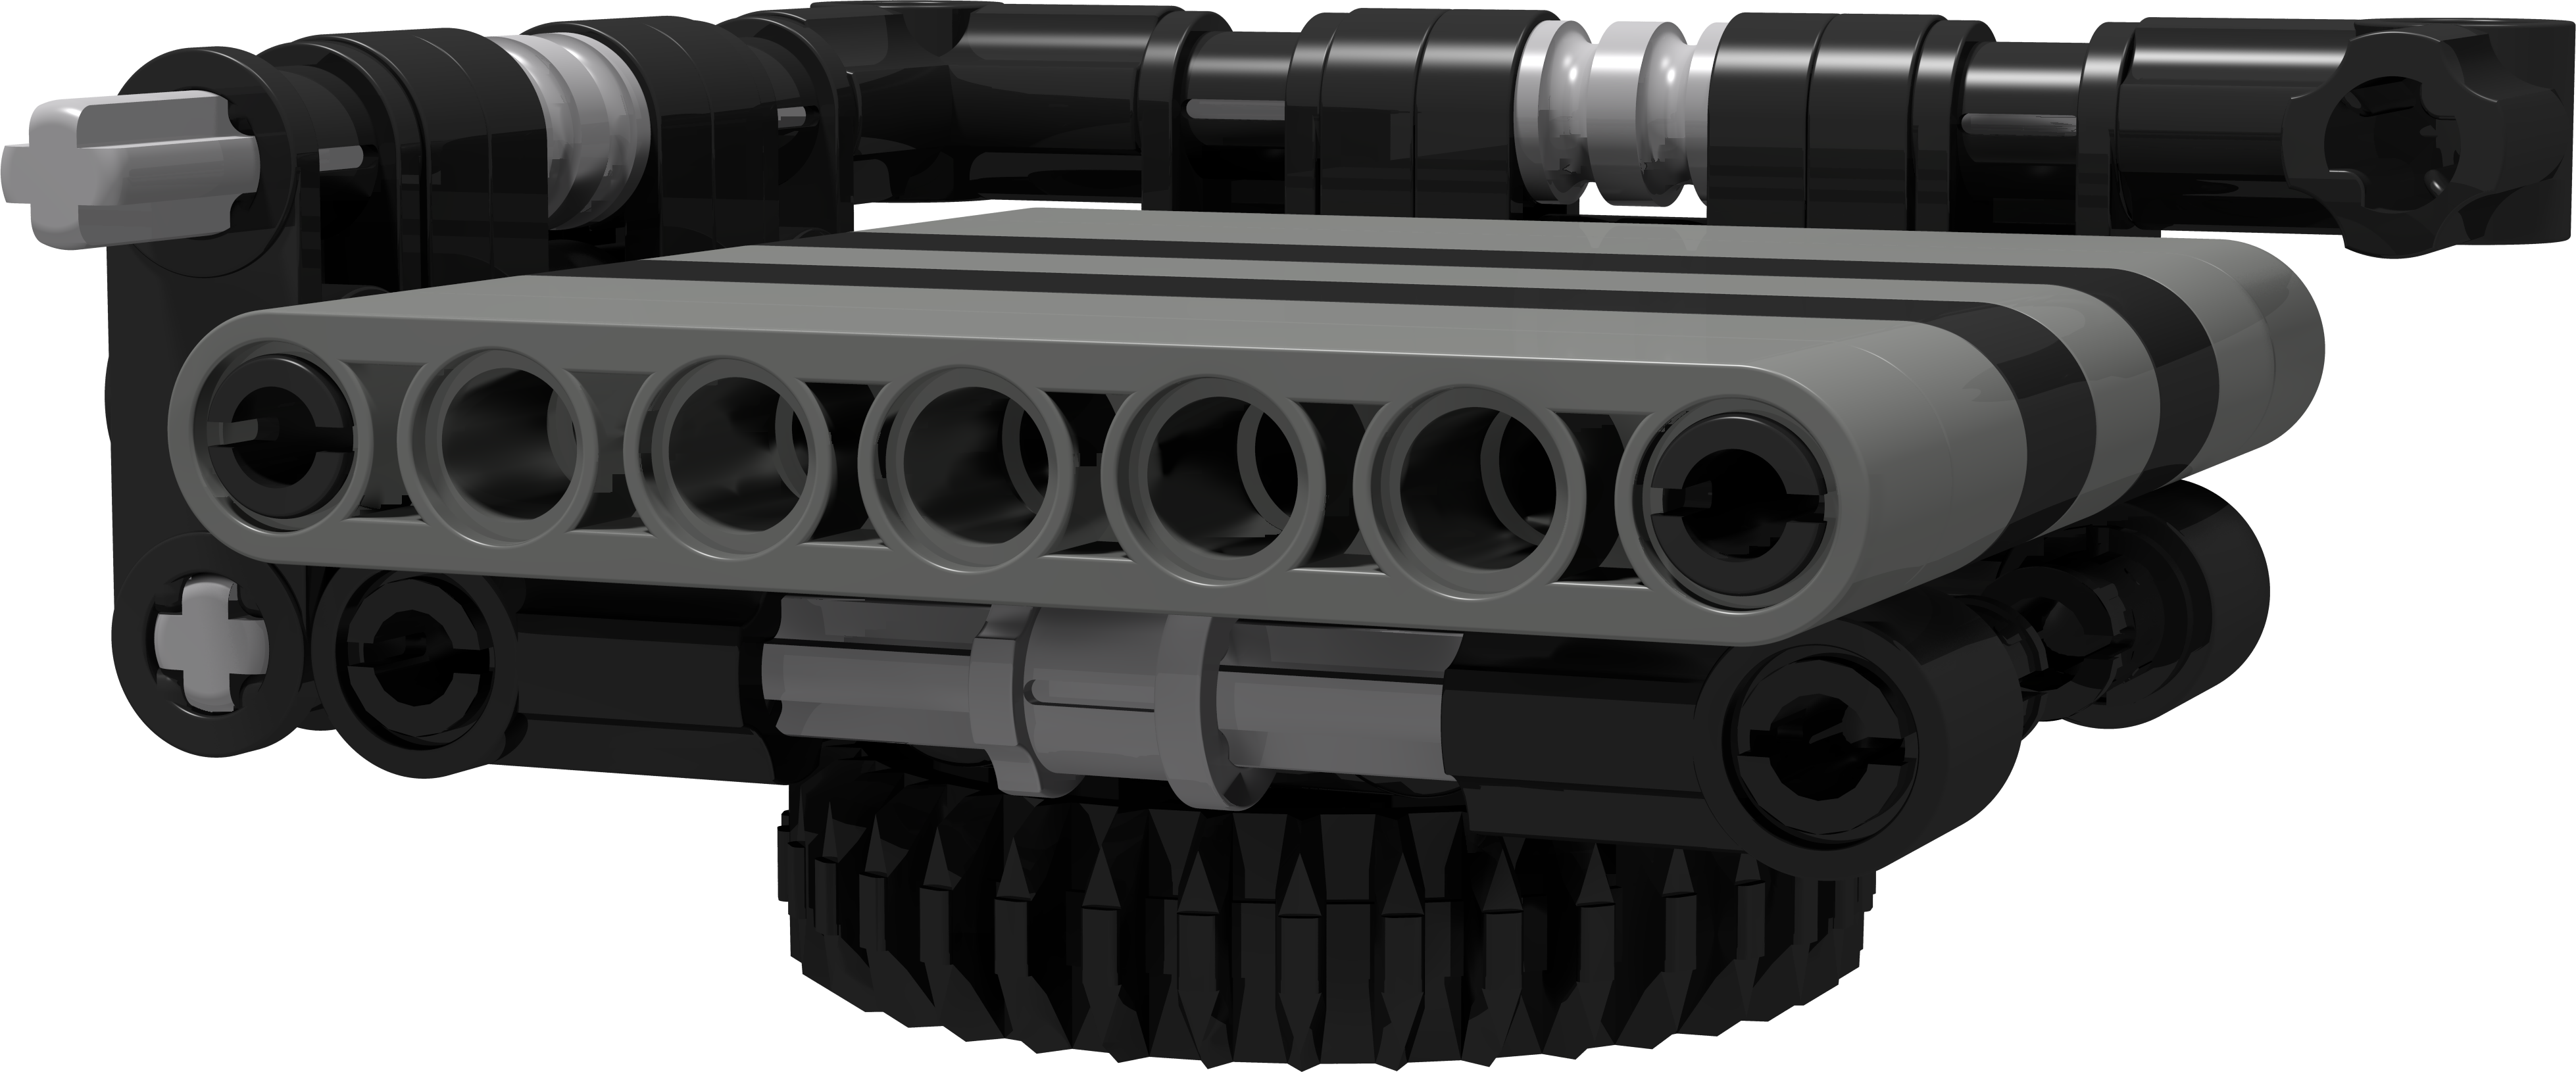
\includegraphics[width=0.4\textwidth]{Resources/Images/rdrCradle.png}
		\caption{A view of the cradle with some parts removed}
		\label{fig:rdrCradle}
	\end{figure}
	
	The wall will have a semi-circular profile to allow the Cube to rotate smoothly out of the base of the cradle as demonstrated in Figures \ref{fig:dwgCradleCurvedEdgeNormal} and \ref{fig:dwgCradleCurvedEdgeTilted}. The method for rotating the cradle is for it to be mounted directly onto the rotor of a large motor. This gives it stability from the secure mount, high rotational velocity because there is no gearing down, and it will be accurate due to the in-built tachometer which provides \enquote{precise control to within one degree of accuracy} \cite{Lego}. Figure \ref{fig:dwgCradleProfileV1} shows the cradle mounted via a large gear to give the cradle sufficient clearance from the motor's body.
    
    \begin{figure}[H]
    	\centering
 	   	\begin{subfigure}[b]{0.2\textwidth}
    		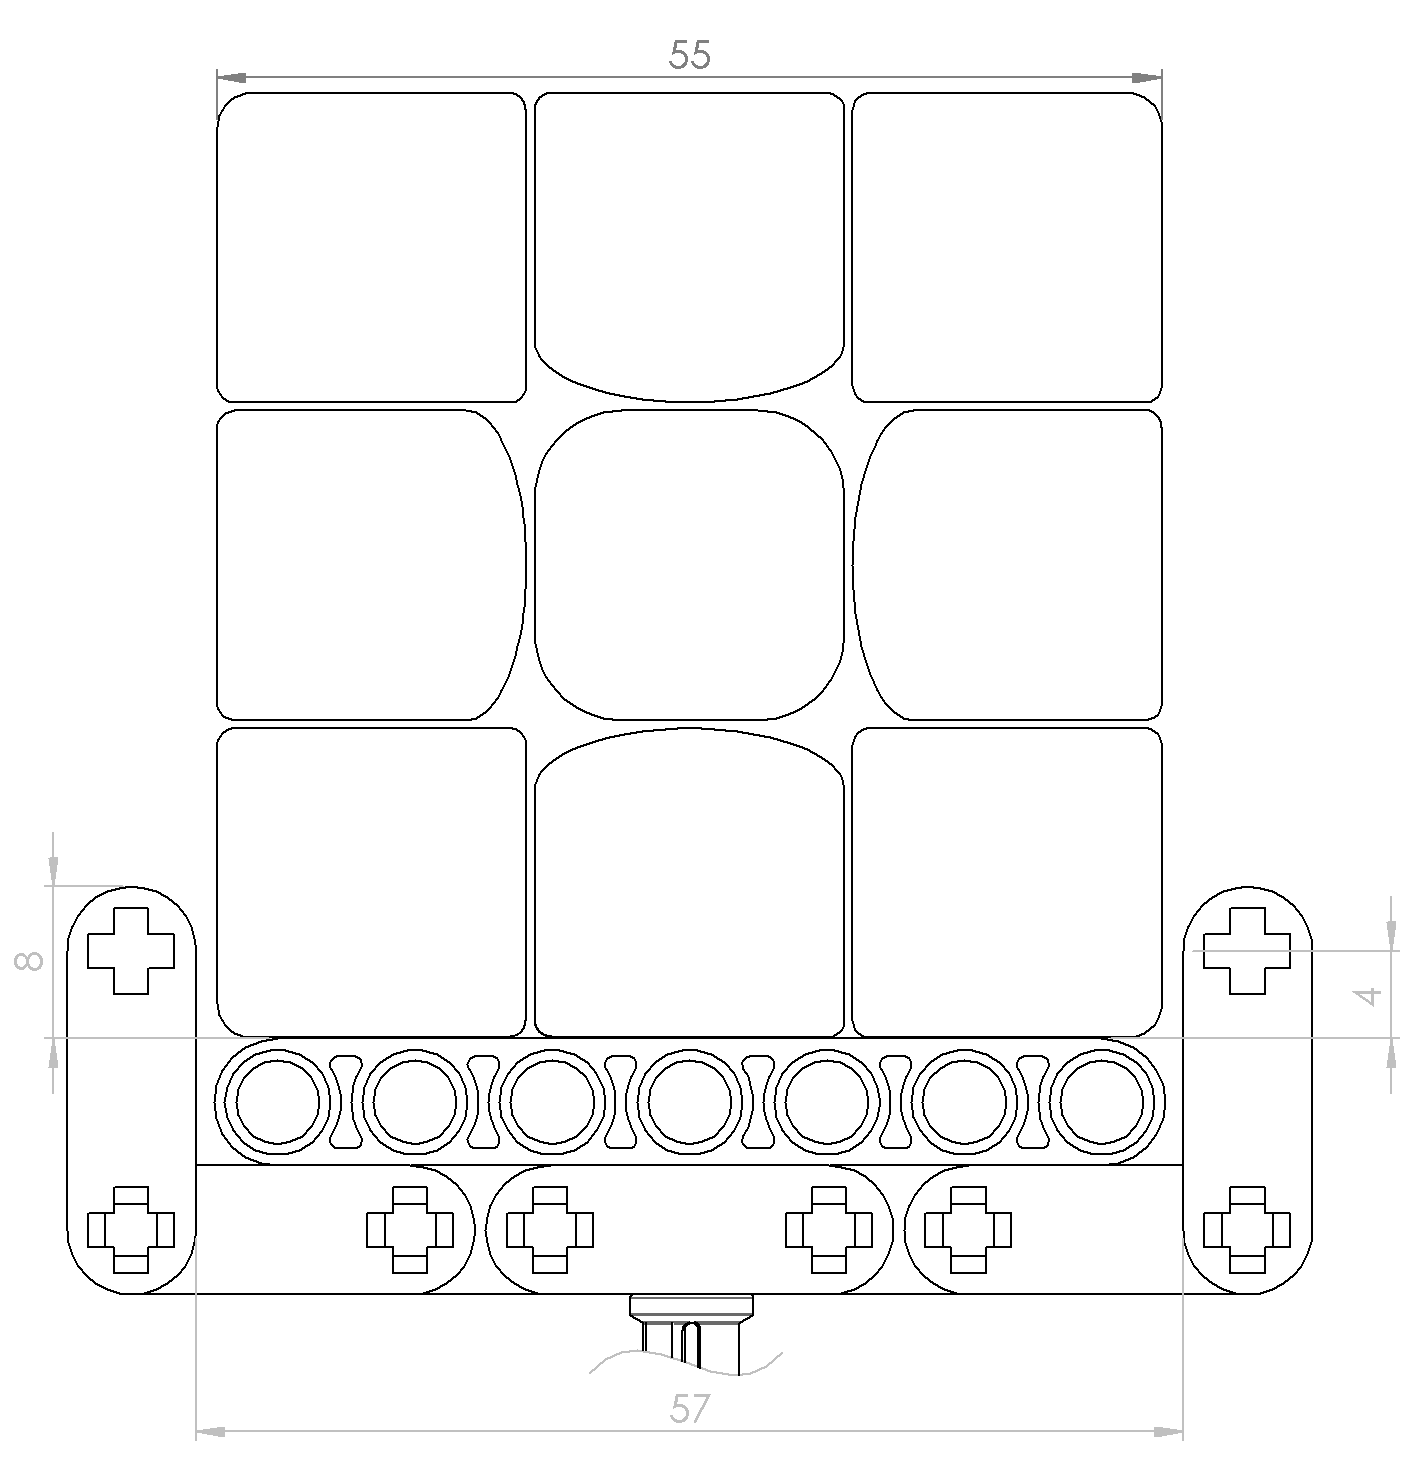
\includegraphics[width=\textwidth]{Resources/Images/dwgCradleCurvedEdgeNormal.png}
    		\caption{Resting position}
    		\label{fig:dwgCradleCurvedEdgeNormal}
    	\end{subfigure}
    	\hspace{10mm}
    	\begin{subfigure}[b]{0.2\textwidth}
    		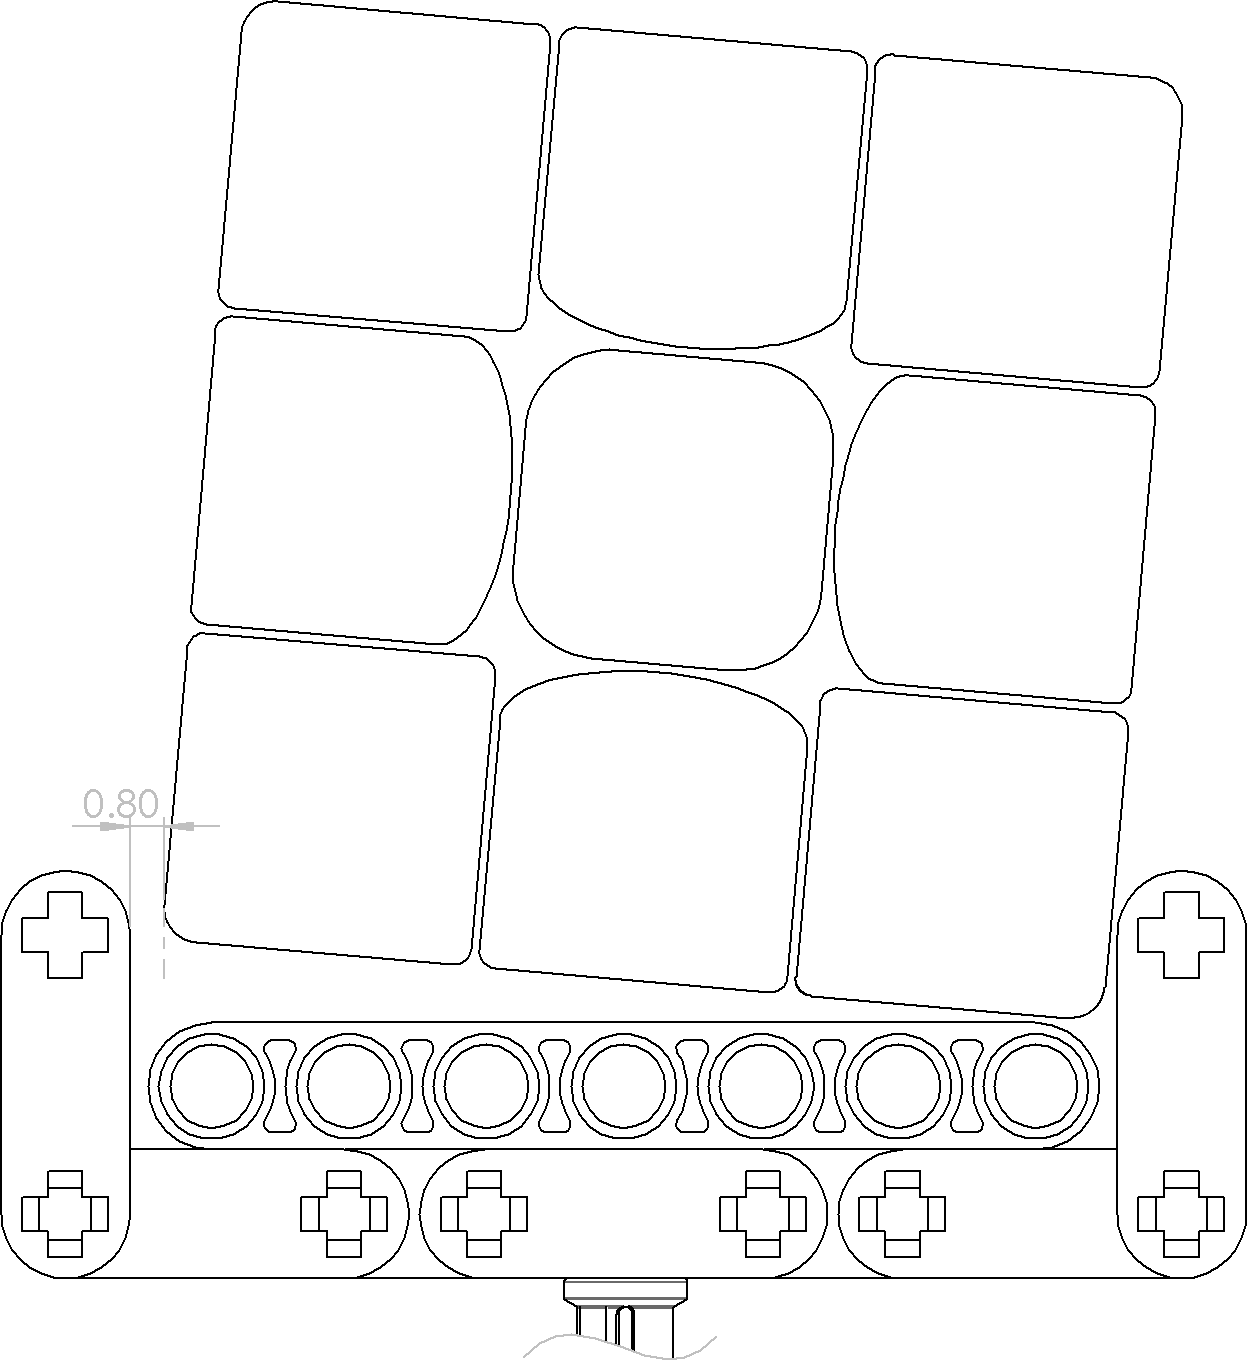
\includegraphics[width=\textwidth]{Resources/Images/dwgCradleCurvedEdgeTilted.png}
    		\caption{Starting an \move{x}}
    		\label{fig:dwgCradleCurvedEdgeTilted}
    	\end{subfigure}
	    \hspace{10mm}
	    \begin{subfigure}[b]{0.4\textwidth}
	    	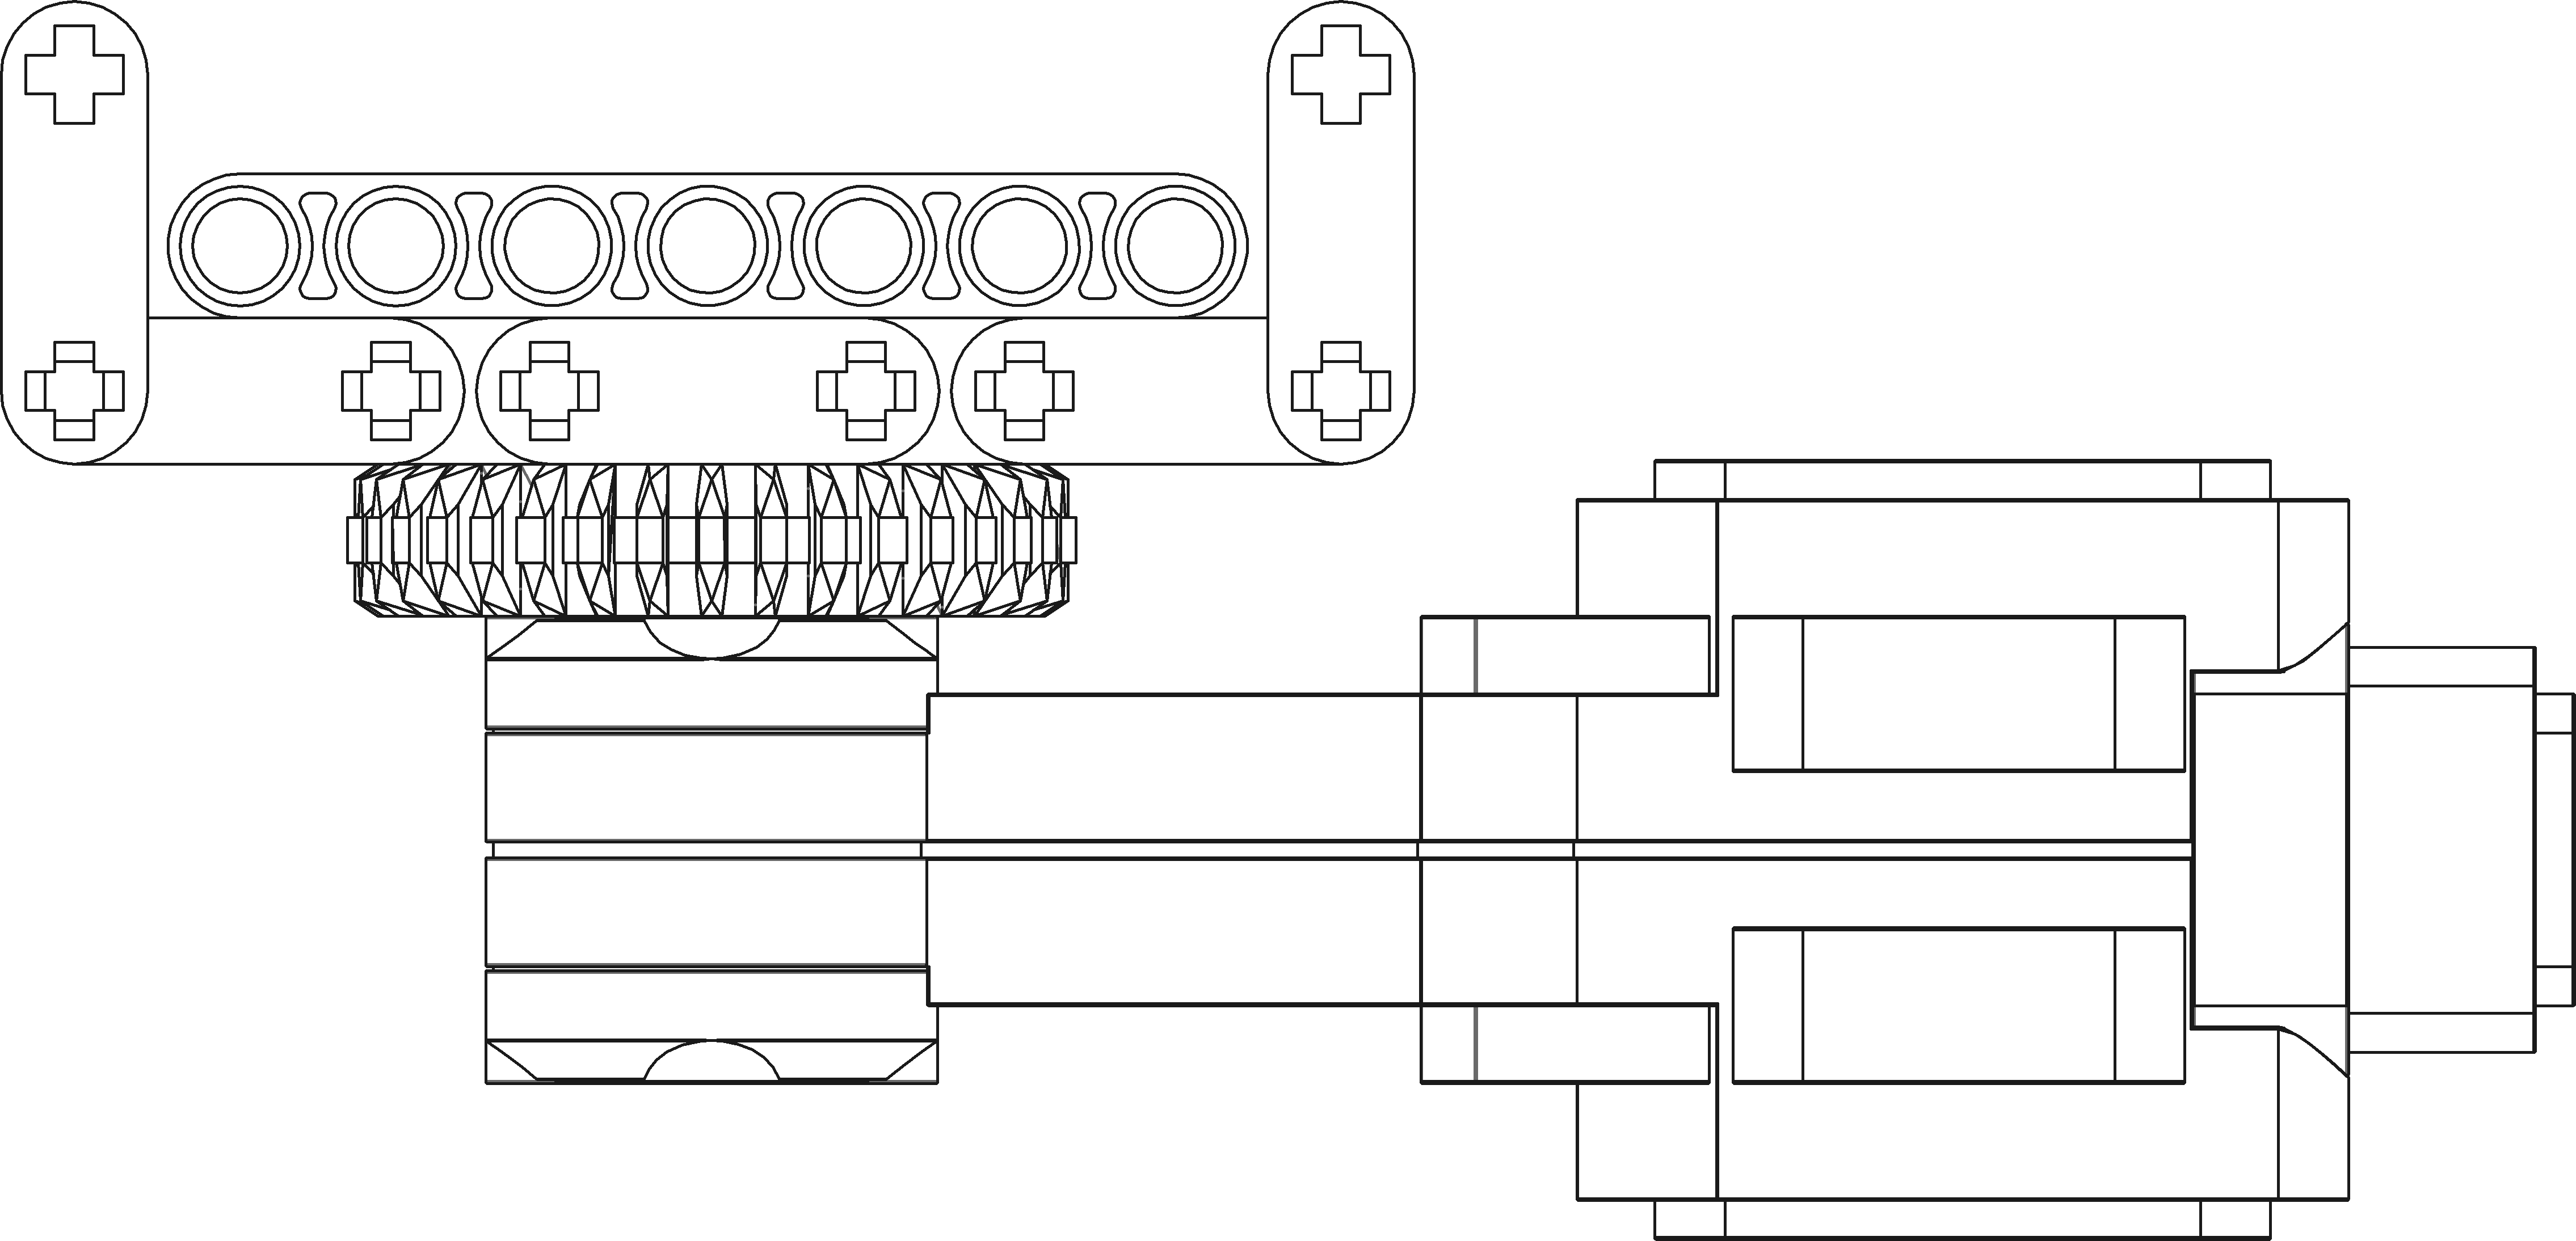
\includegraphics[width=\textwidth]{Resources/Images/dwgCradleProfileV1.png}
	    	\caption{The cradle is mounted on a motor}
	    	\label{fig:dwgCradleProfileV1}
	    \end{subfigure}
    	\caption{Technical drawings showing the the Cube, the cradle, and its mounting}
    	\label{fig:CradleDrawings}
    \end{figure}    
    
    Figure \ref{fig:rdrCradleMountedRotor} is a rendered image of the aforementioned 3D model. It shows how the cradle and the motor will be supported by a framework which will link to the rest of the MkI.
    
    \begin{figure}[H]
    	\centering
   		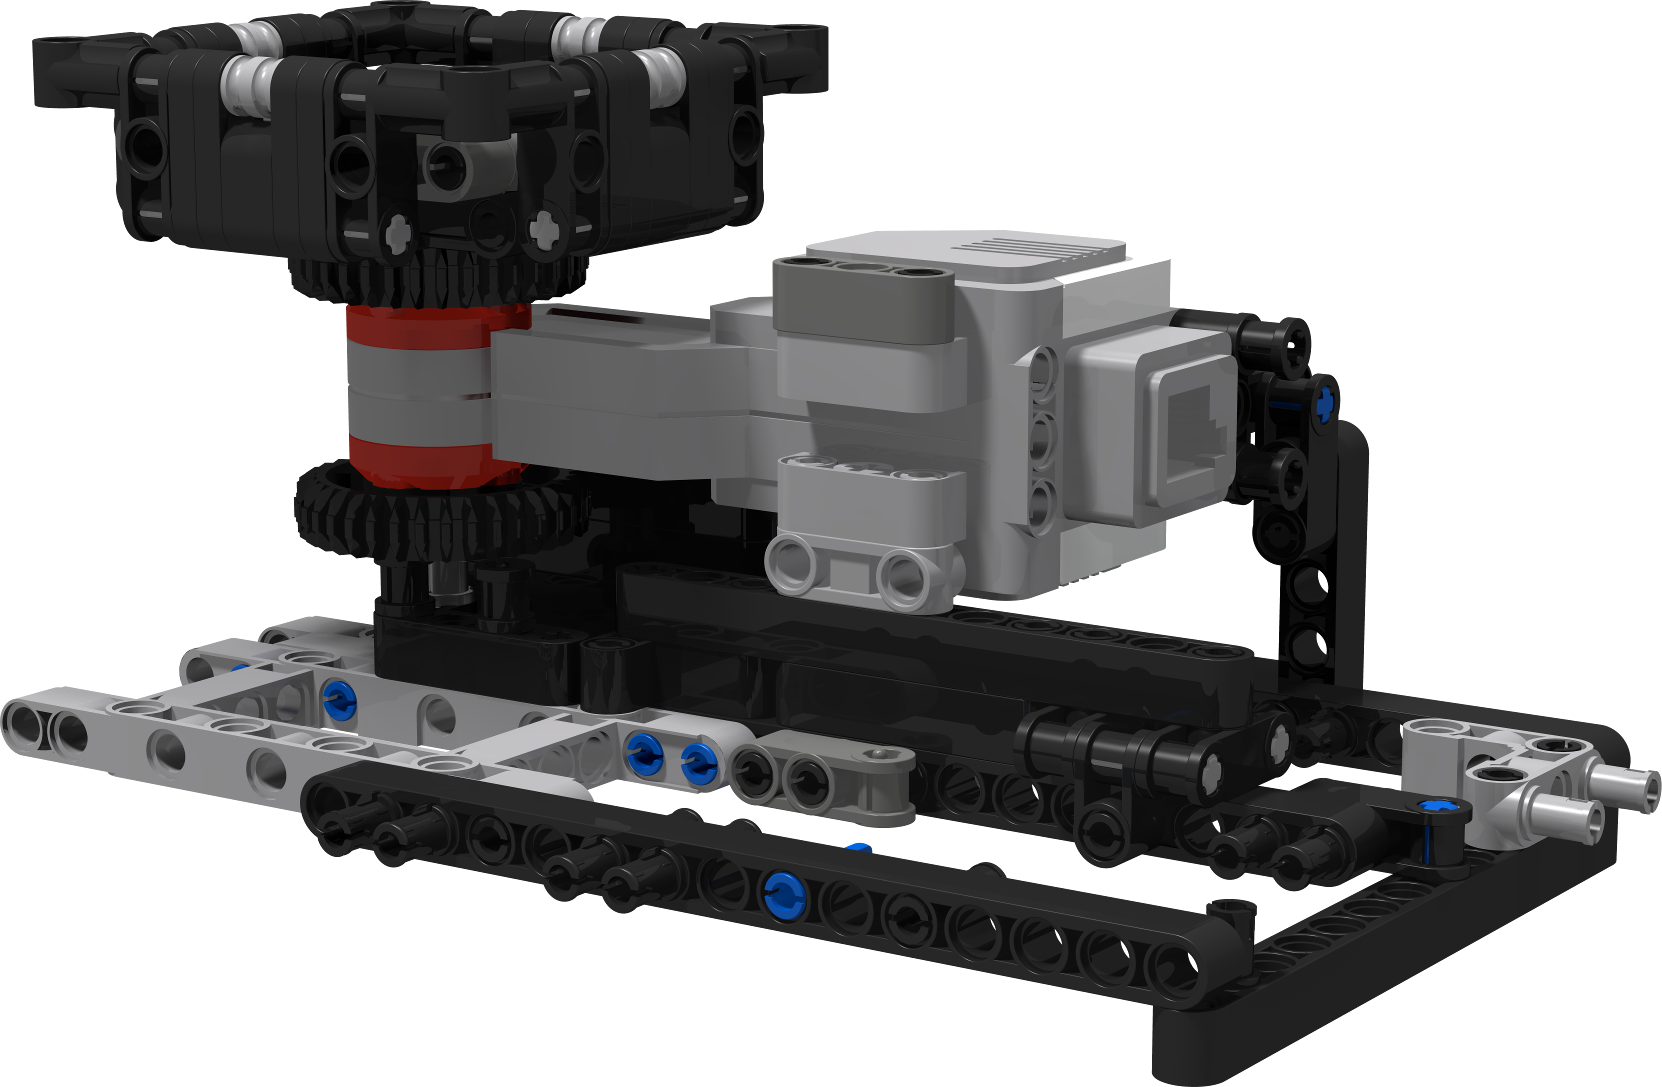
\includegraphics[width=0.5\textwidth]{Resources/Images/rdrCradleMountedRotor.png}
   		\caption{A render showing the original cradle mount design}
   		\label{fig:rdrCradleMountedRotor}
    \end{figure}
    
    \subsection{X-Move Arm}
    
    The rotating arm which will apply the force $F$ shown in Figure \ref{fig:dwgCubeFreeBodyDiagram} to cause the Cube to pivot about the opposite cradle wall as shown in Figure \ref{fig:dwgRotatingArm}. On one end of the arm there will be a wheel with a rubber tire to provide enough friction to tip the Cube over, and the other end will have a set of guards which can hold the top two slices of the Cube in place when performing a \move{D} or \move{d'}. The length of the guards will be staggered so that they do not collide with the cradle mid-rotation. Small right-angled pieces have been used to reinforced the corners of the arm, and liftarms will be used to hold the guards together to resist the outwards pushing force exerted on them by the rotating Cube.
    
    \begin{figure}[H]
    	\centering
   		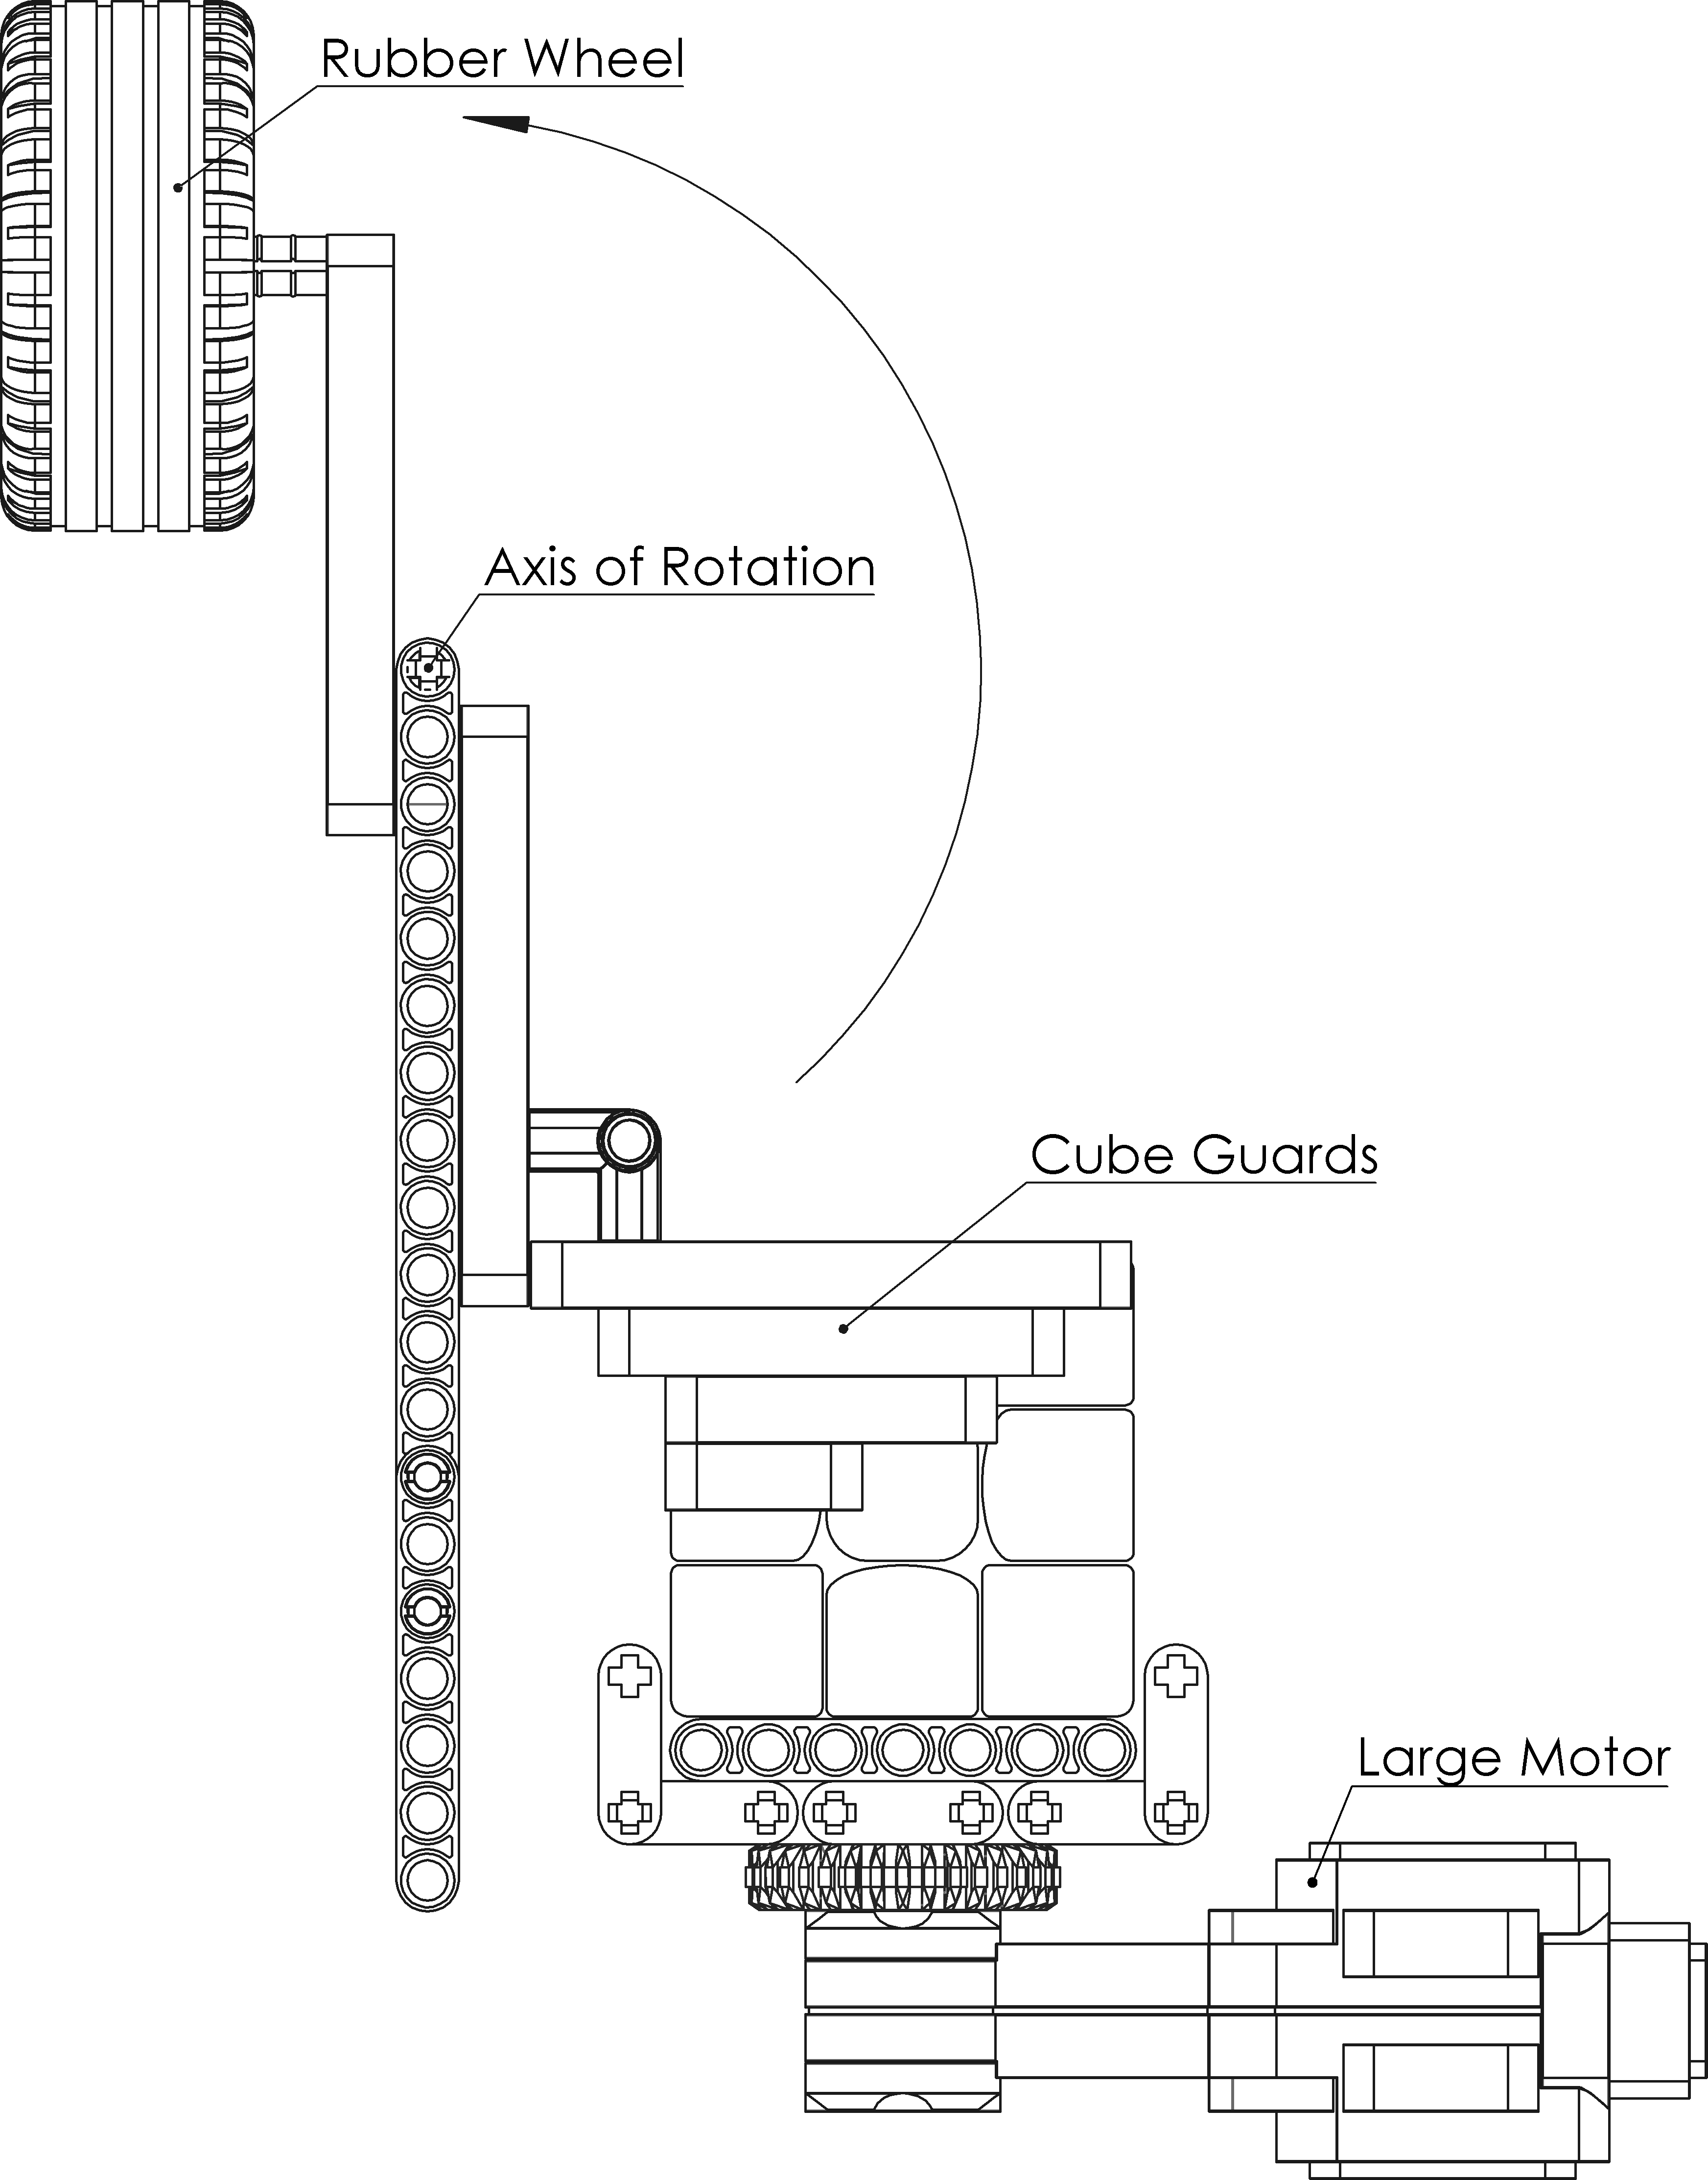
\includegraphics[width=0.4\textwidth]{Resources/Images/dwgRotatingArm.png}
   		\caption{The rotating arm used to flip the Cube}
   		\label{fig:dwgRotatingArm}
    \end{figure}

	Three primary positions of the arm can be seen below in Figure \ref{fig:rdrXMoveArmV1}. Figure \ref{fig:rdrXMoveArmV1_1} shows the \enquote{guarded} position of the arm, where the guards are positioned either side of the Cube to hold the \slice{l-r} and the \face{U} in place when performing a \move{D}, \move{D'} or \move{D2}. The two liftarms \legopiece{40490} that have been attached to the upper part of the guards to hold them together are visible just above the right-angled connectors \legopiece{55615} used to attach the guards to the arm. The guard assembly is attached to a central axle which is rotated by the large motor visible at the far side of the model. The entire assembly's weight is balanced sufficiently well to ensure that there is a smooth rotation about the axle and no unnecessary strain is placed on the motor.

	\begin{figure}[H]
		\centering
		\begin{subfigure}[b]{0.22193\textwidth}
			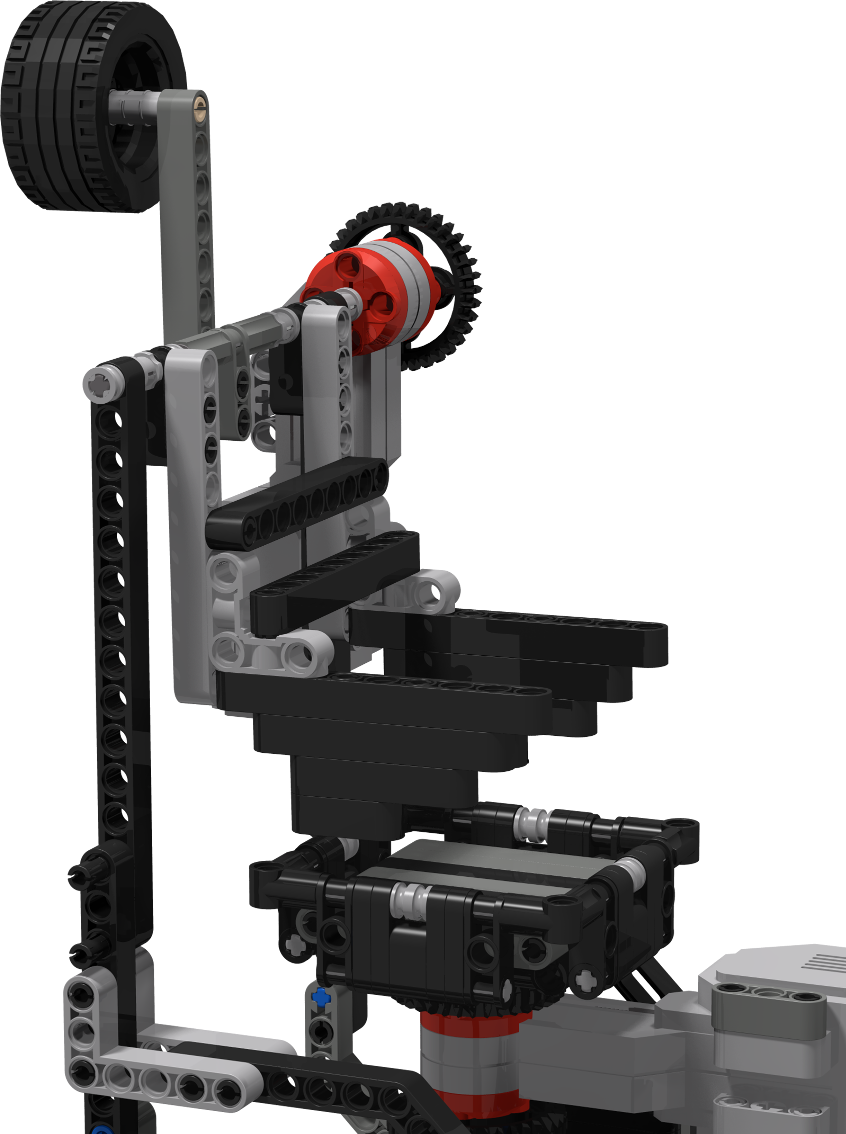
\includegraphics[width=\textwidth]{Resources/Images/rdrXMoveArmV1_1.png}
			\caption{Guarded position}
			\label{fig:rdrXMoveArmV1_1}
		\end{subfigure}
		\hspace{10mm}
		\begin{subfigure}[b]{0.22\textwidth}
			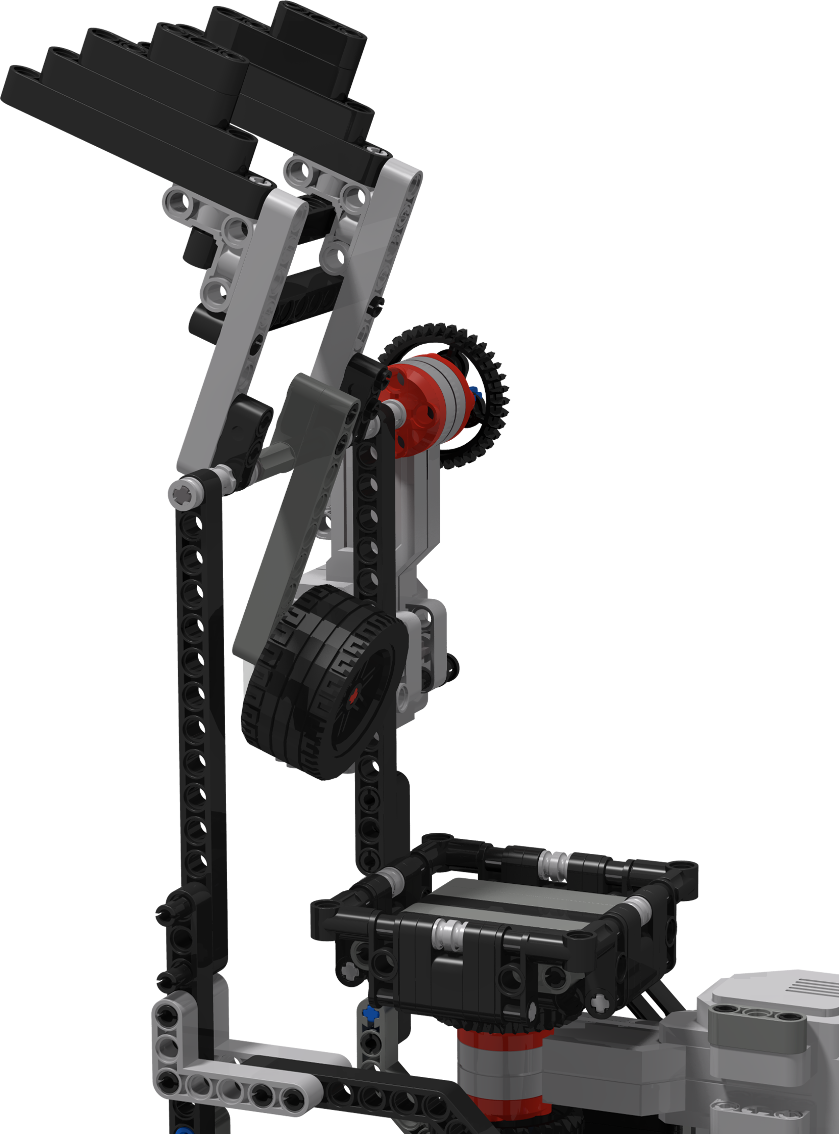
\includegraphics[width=\textwidth]{Resources/Images/rdrXMoveArmV1_2.png}
			\caption{Starting the \move{X}}
			\label{fig:rdrXMoveArmV1_2}
		\end{subfigure}
		\hspace{10mm}
		\begin{subfigure}[b]{0.30811\textwidth}
			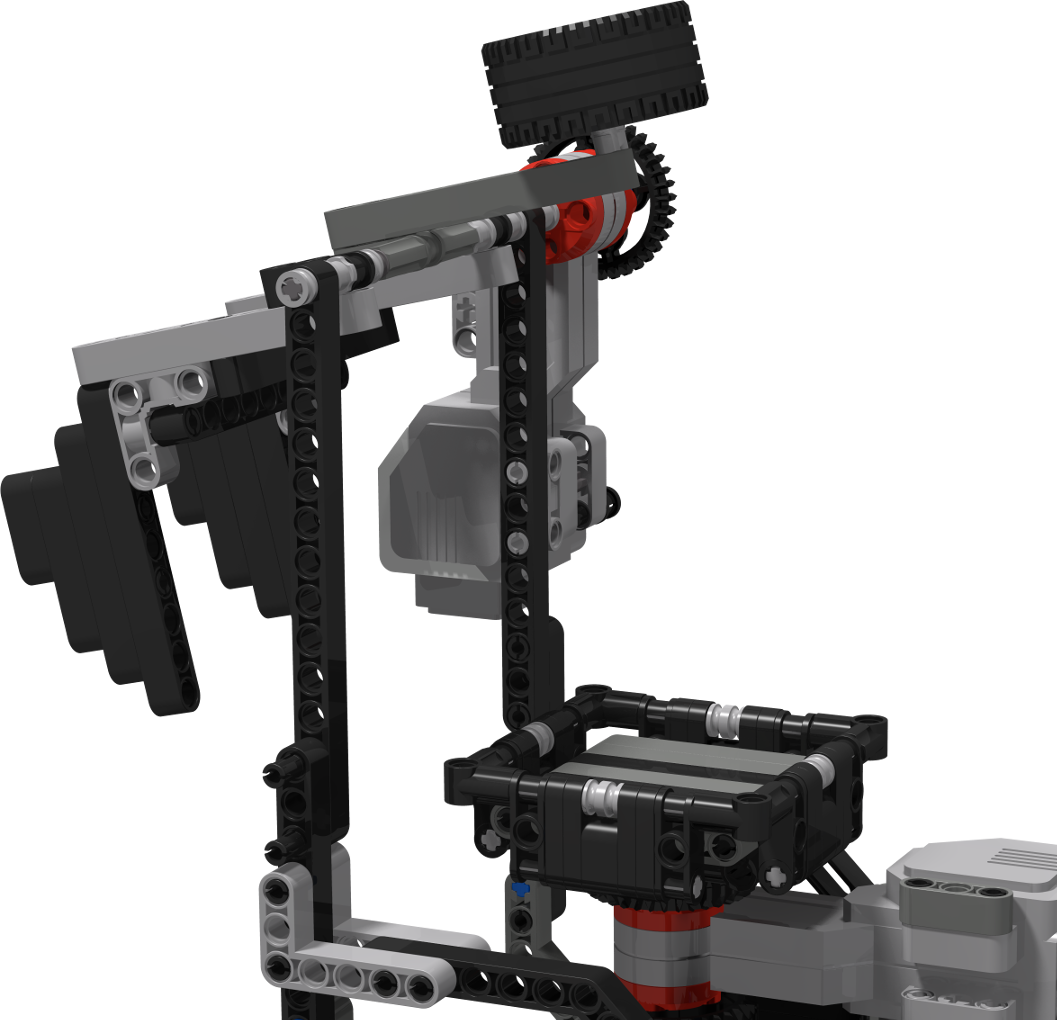
\includegraphics[width=\textwidth]{Resources/Images/rdrXMoveArmV1_3.png}
			\caption{Unguarded position}
			\label{fig:rdrXMoveArmV1_3}
		\end{subfigure}
		\caption{Three different positions of the X-Move Arm}
		\label{fig:rdrXMoveArmV1}
	\end{figure}
	

	\subsection{Colour Sensor}
	
	\subsubsection{\lego Design}
	
	The colour sensor will be powered by the medium motor and a gear train which ends with a worm gear \legopiece{4716} and rack \legopiece{3743}. The rack will be directly connected to a liftarm which has two long parallel shafts \legopiece{3708} mounted above it, both of which feed through a liftarm attached to the main frame of the MkI. These shafts are the only fixed mounting points for the whole colour sensor assembly - the worm gears and rack provide lateral movement but little structural support. The distance between the sensor and the top of the Cube will be approximately 8 \si{\milli\metre}. From previous tests and forum data, the optimal distance for the colour sensor appears to be between 10 \si{\milli\metre} and 16 \si{\milli\metre} \cite{UlfR2015}. Although the chosen distance is less than optimal, it ensures that the \enquote{beam} from the colour sensor remains inside the facelets. The accuracy of the readings is not affected.
	
	\begin{figure}[H]
		\centering
		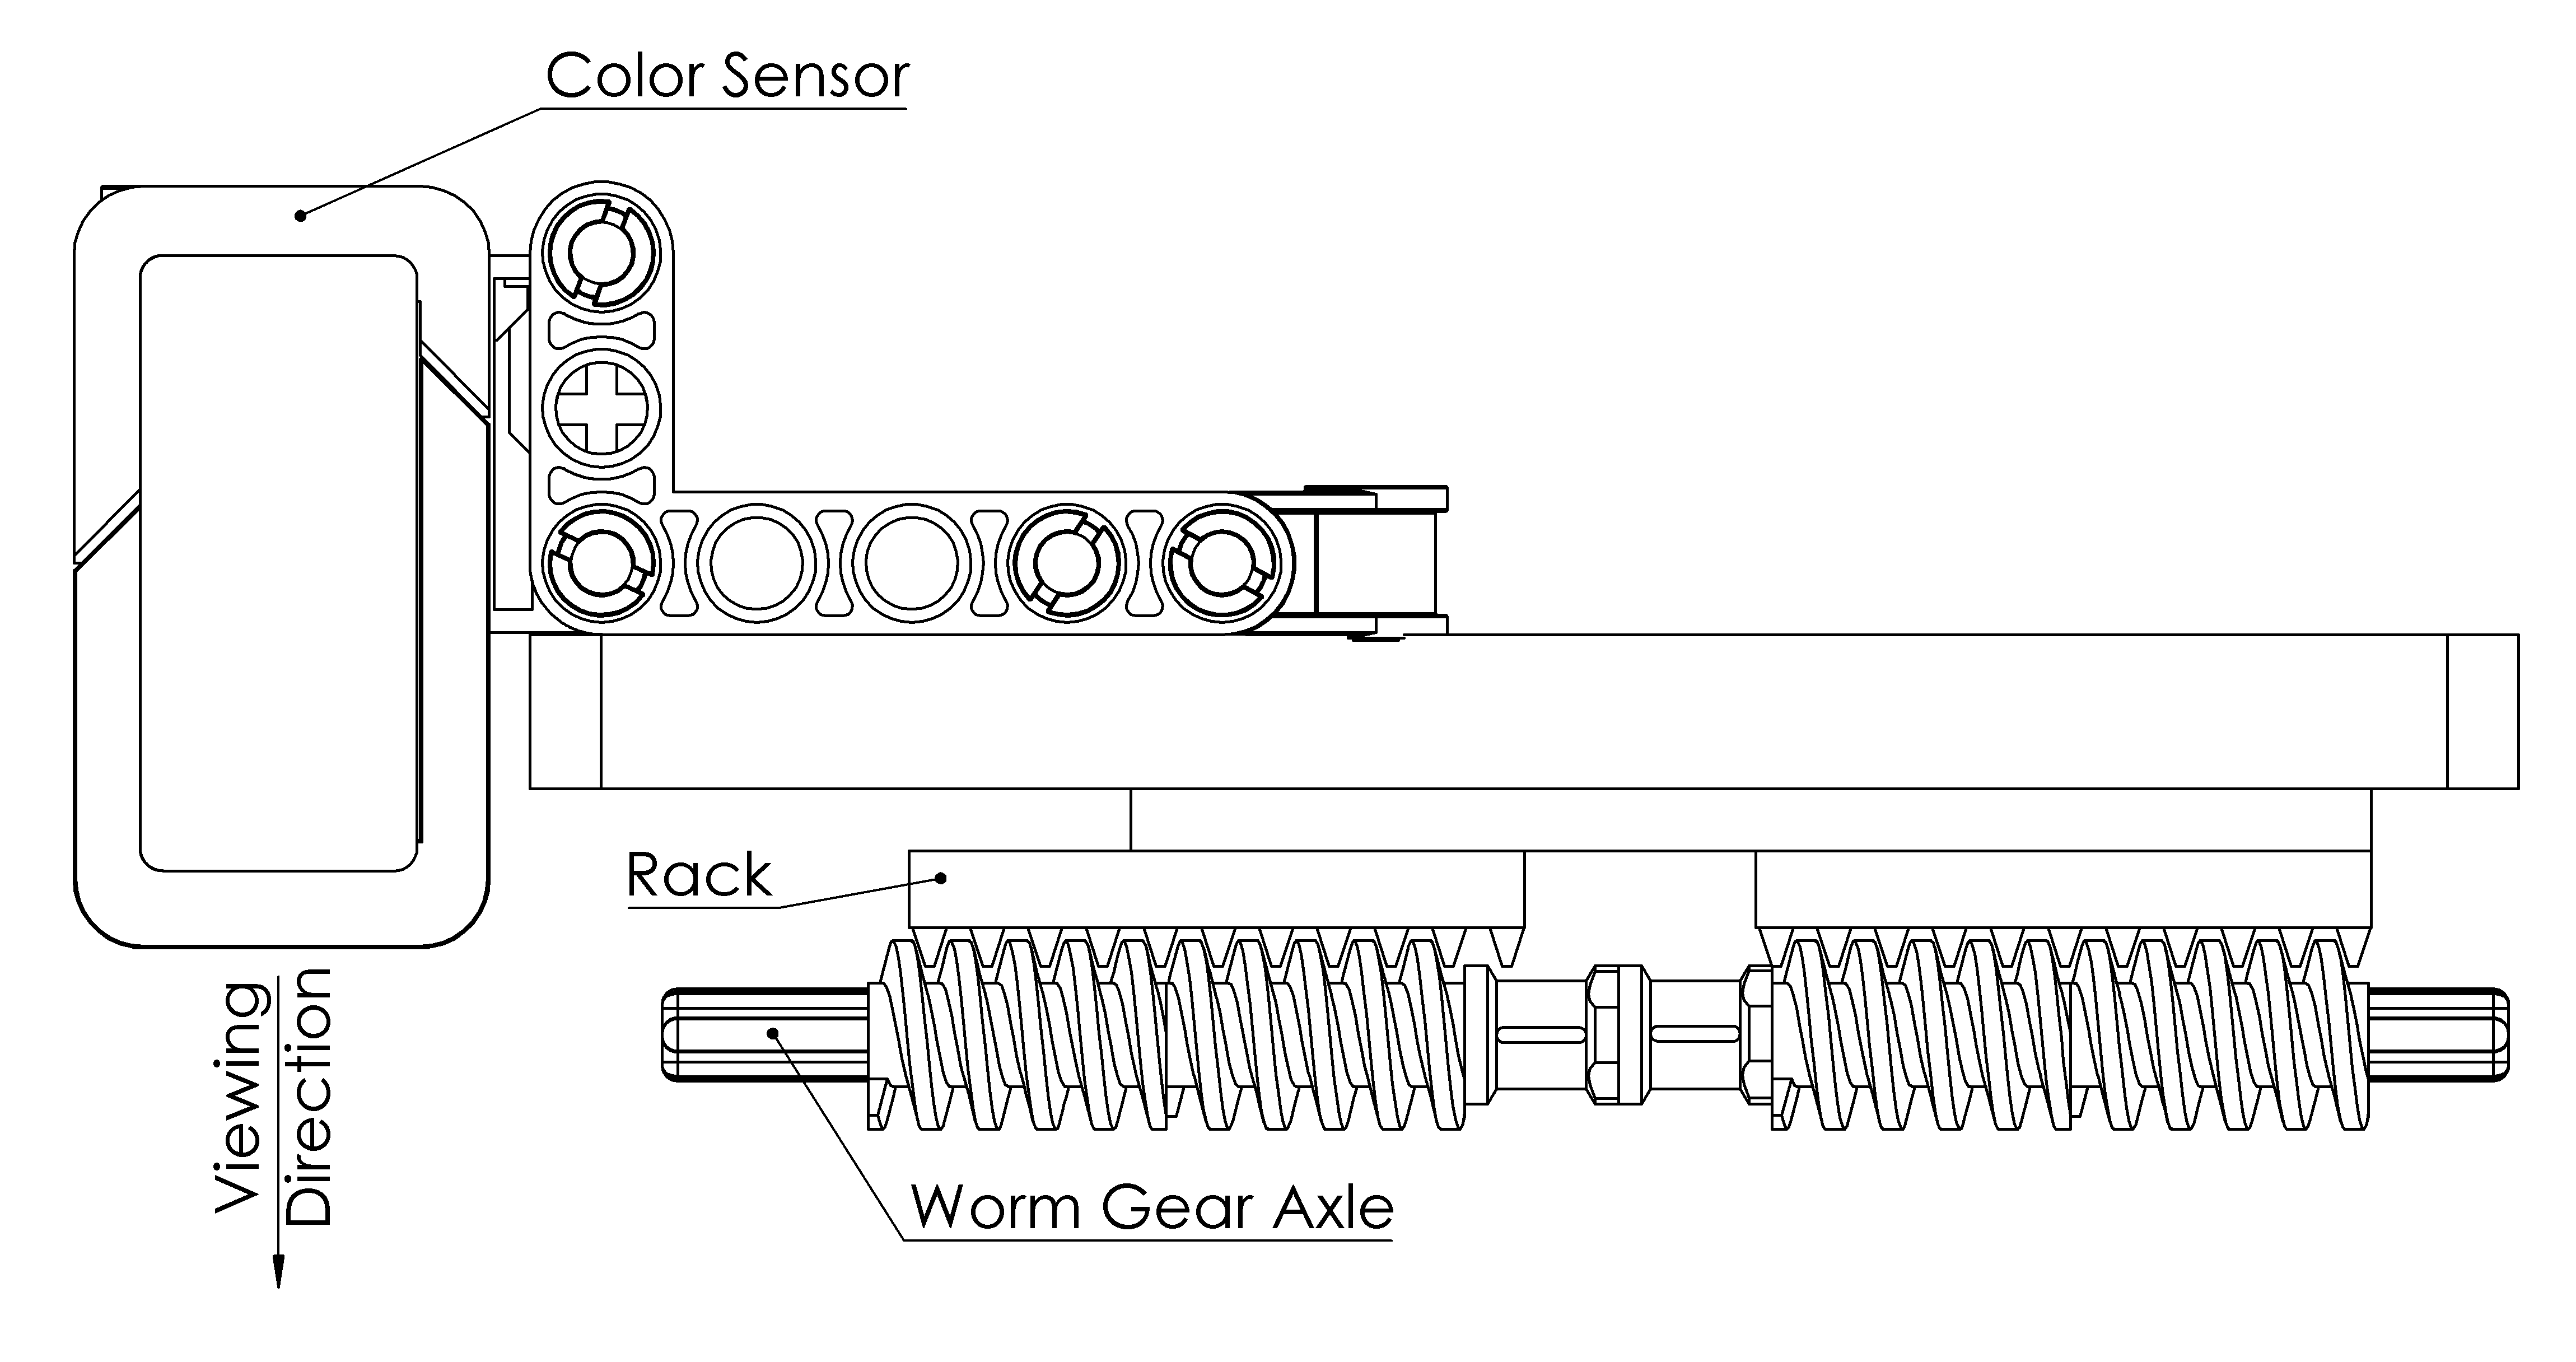
\includegraphics[width=0.5\textwidth]{Resources/Images/dwgColorSensor.png}
		\caption{The colour sensor mounting arm is driven by a set of worm gears}
		\label{fig:dwgColorSensor}
	\end{figure}
	
	The medium motor powers a 24-tooth gear \legopiece{60c01}, which then transmits power to an 8-tooth gear \legopiece{3647}, which is on the same axle as the worm gears. The rotational velocity of the worm gear is 63.75 \si{\radian\per\second} (608 RPM), which means that the lateral velocity of the rack can be calculated to be 0.0662 \si{\meter\per\second}. The time taken for the colour sensor to travel from its neutral position to above the centre facelet is 1.21 \si{\second}.
	
	\begin{figure}[H]
		\centering
		\begin{subfigure}[b]{0.43427\textwidth}
			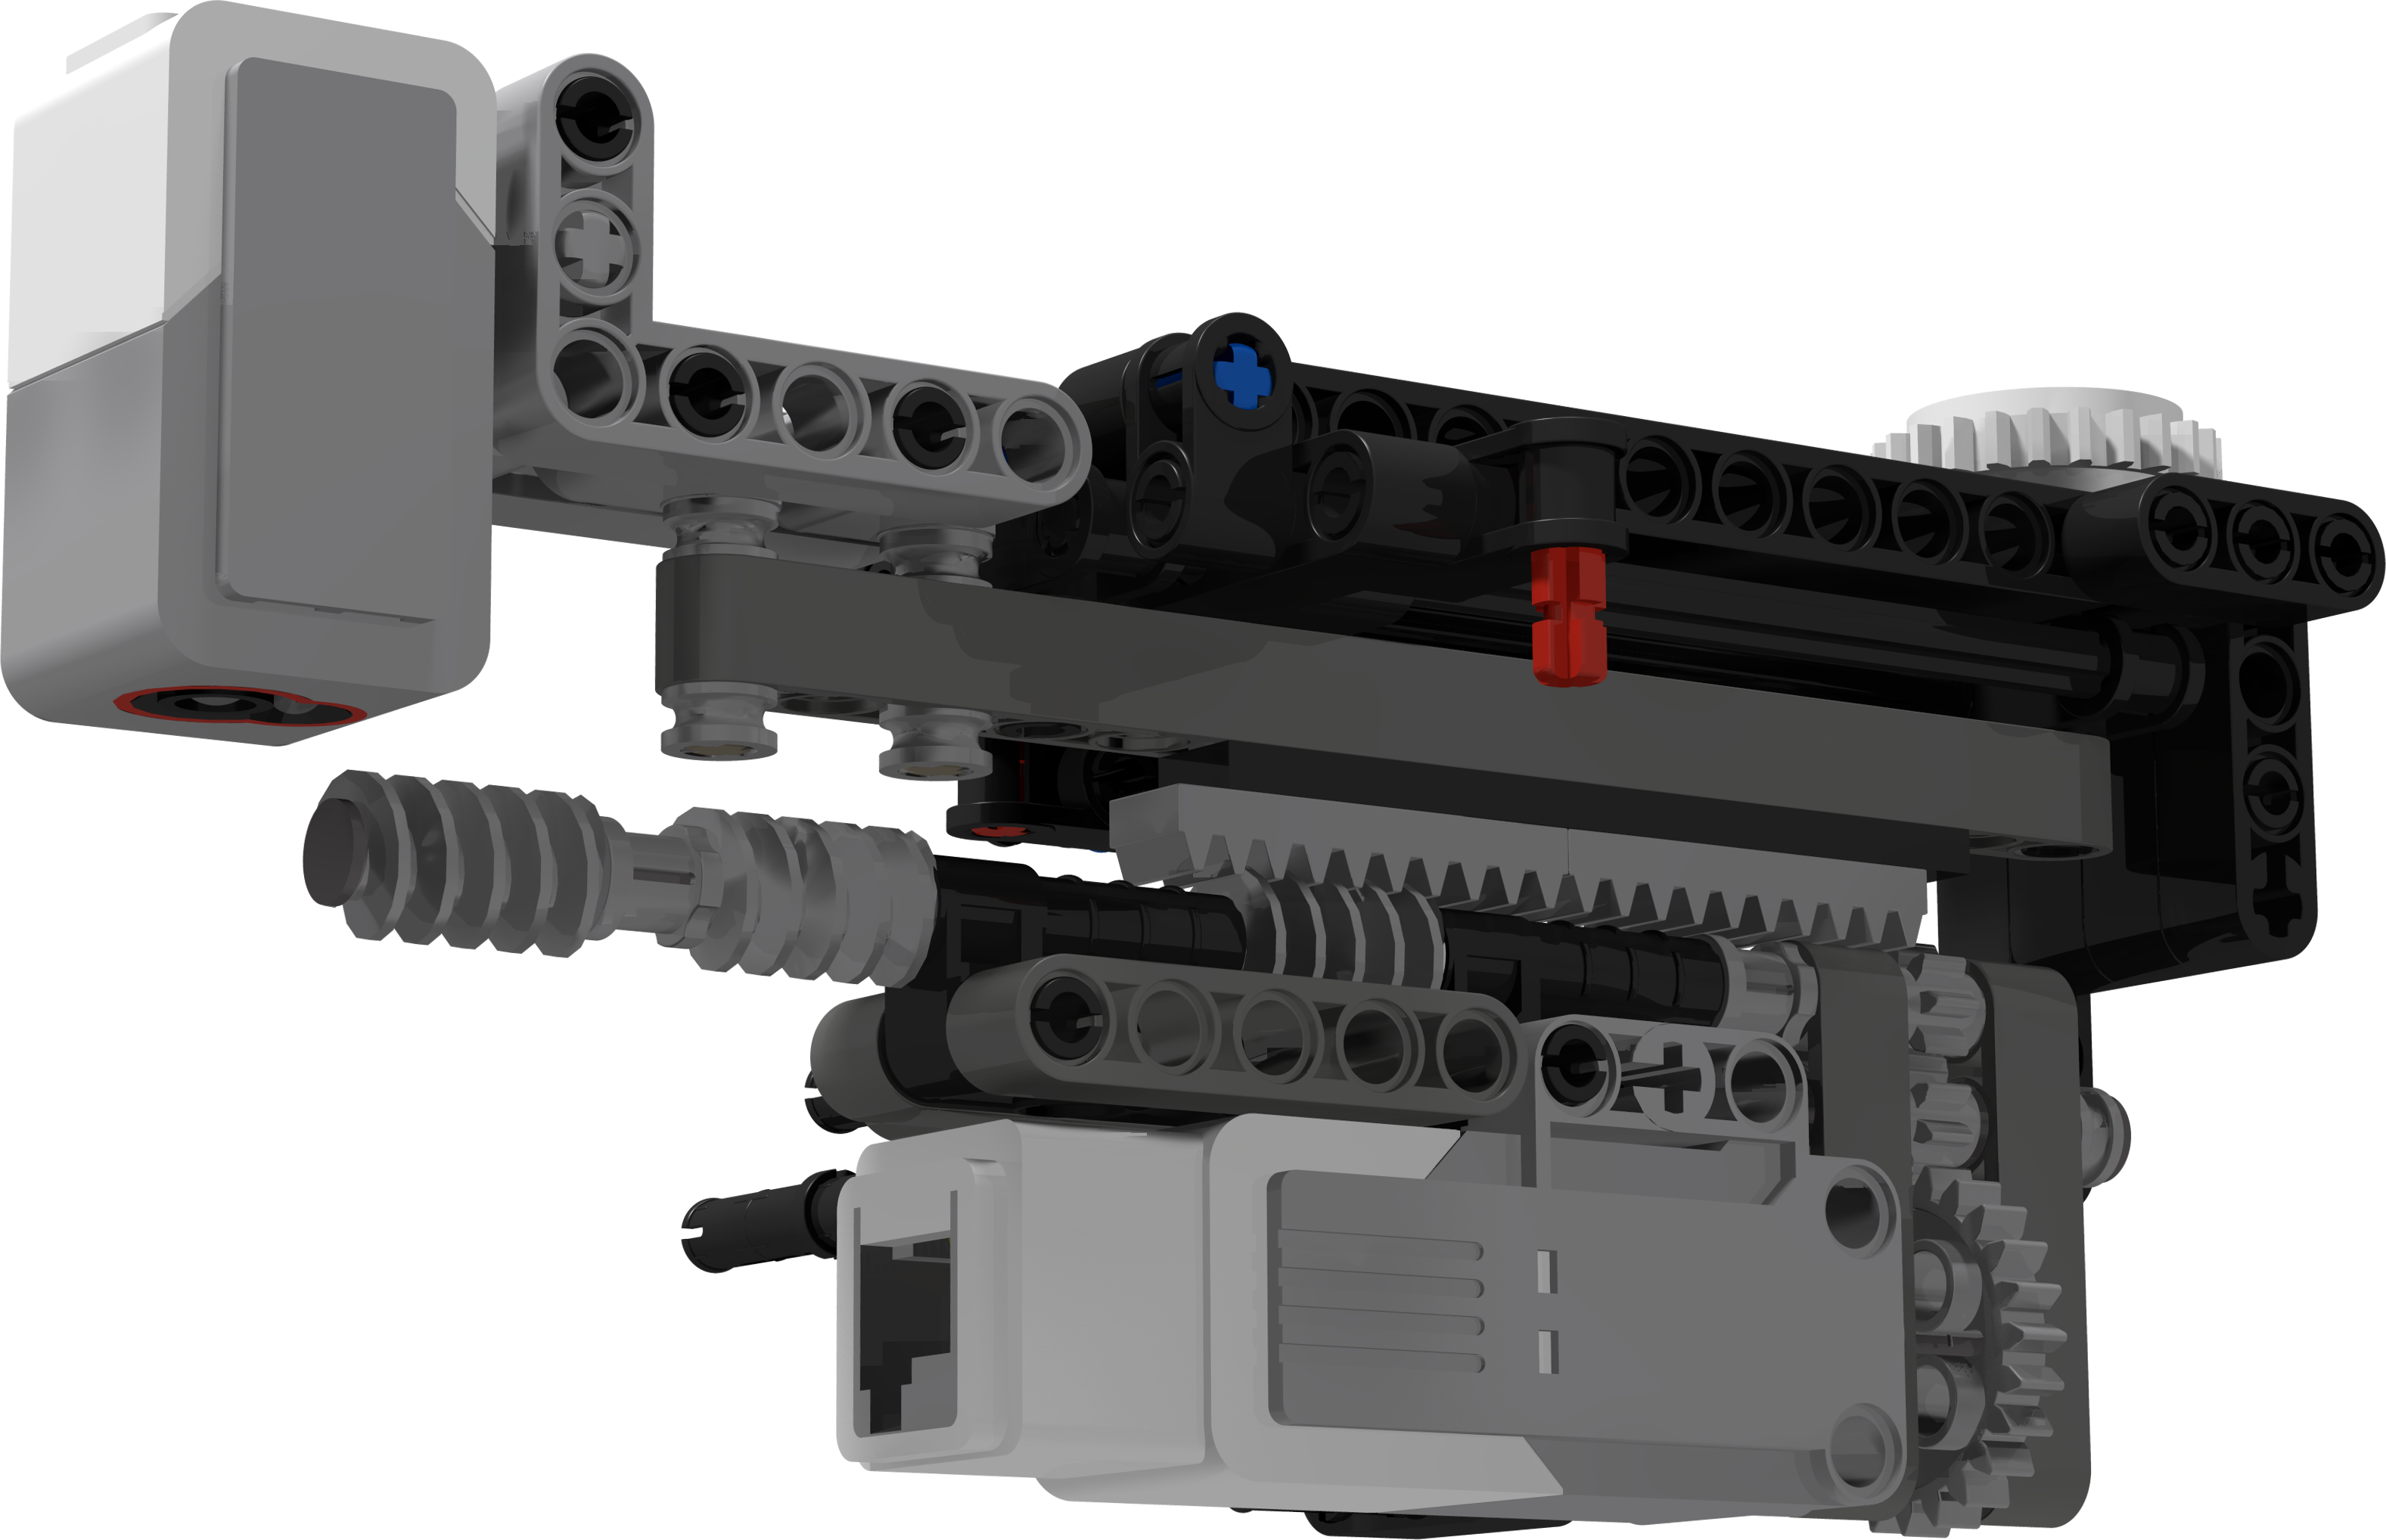
\includegraphics[width=\textwidth]{Resources/Images/rdrColorSensorAssembly.png}
			\caption{A full view of the mechanics}
			\label{fig:rdrColorSensorAssembly}
		\end{subfigure}
		\hspace{10mm}
		\begin{subfigure}[b]{0.4\textwidth}
			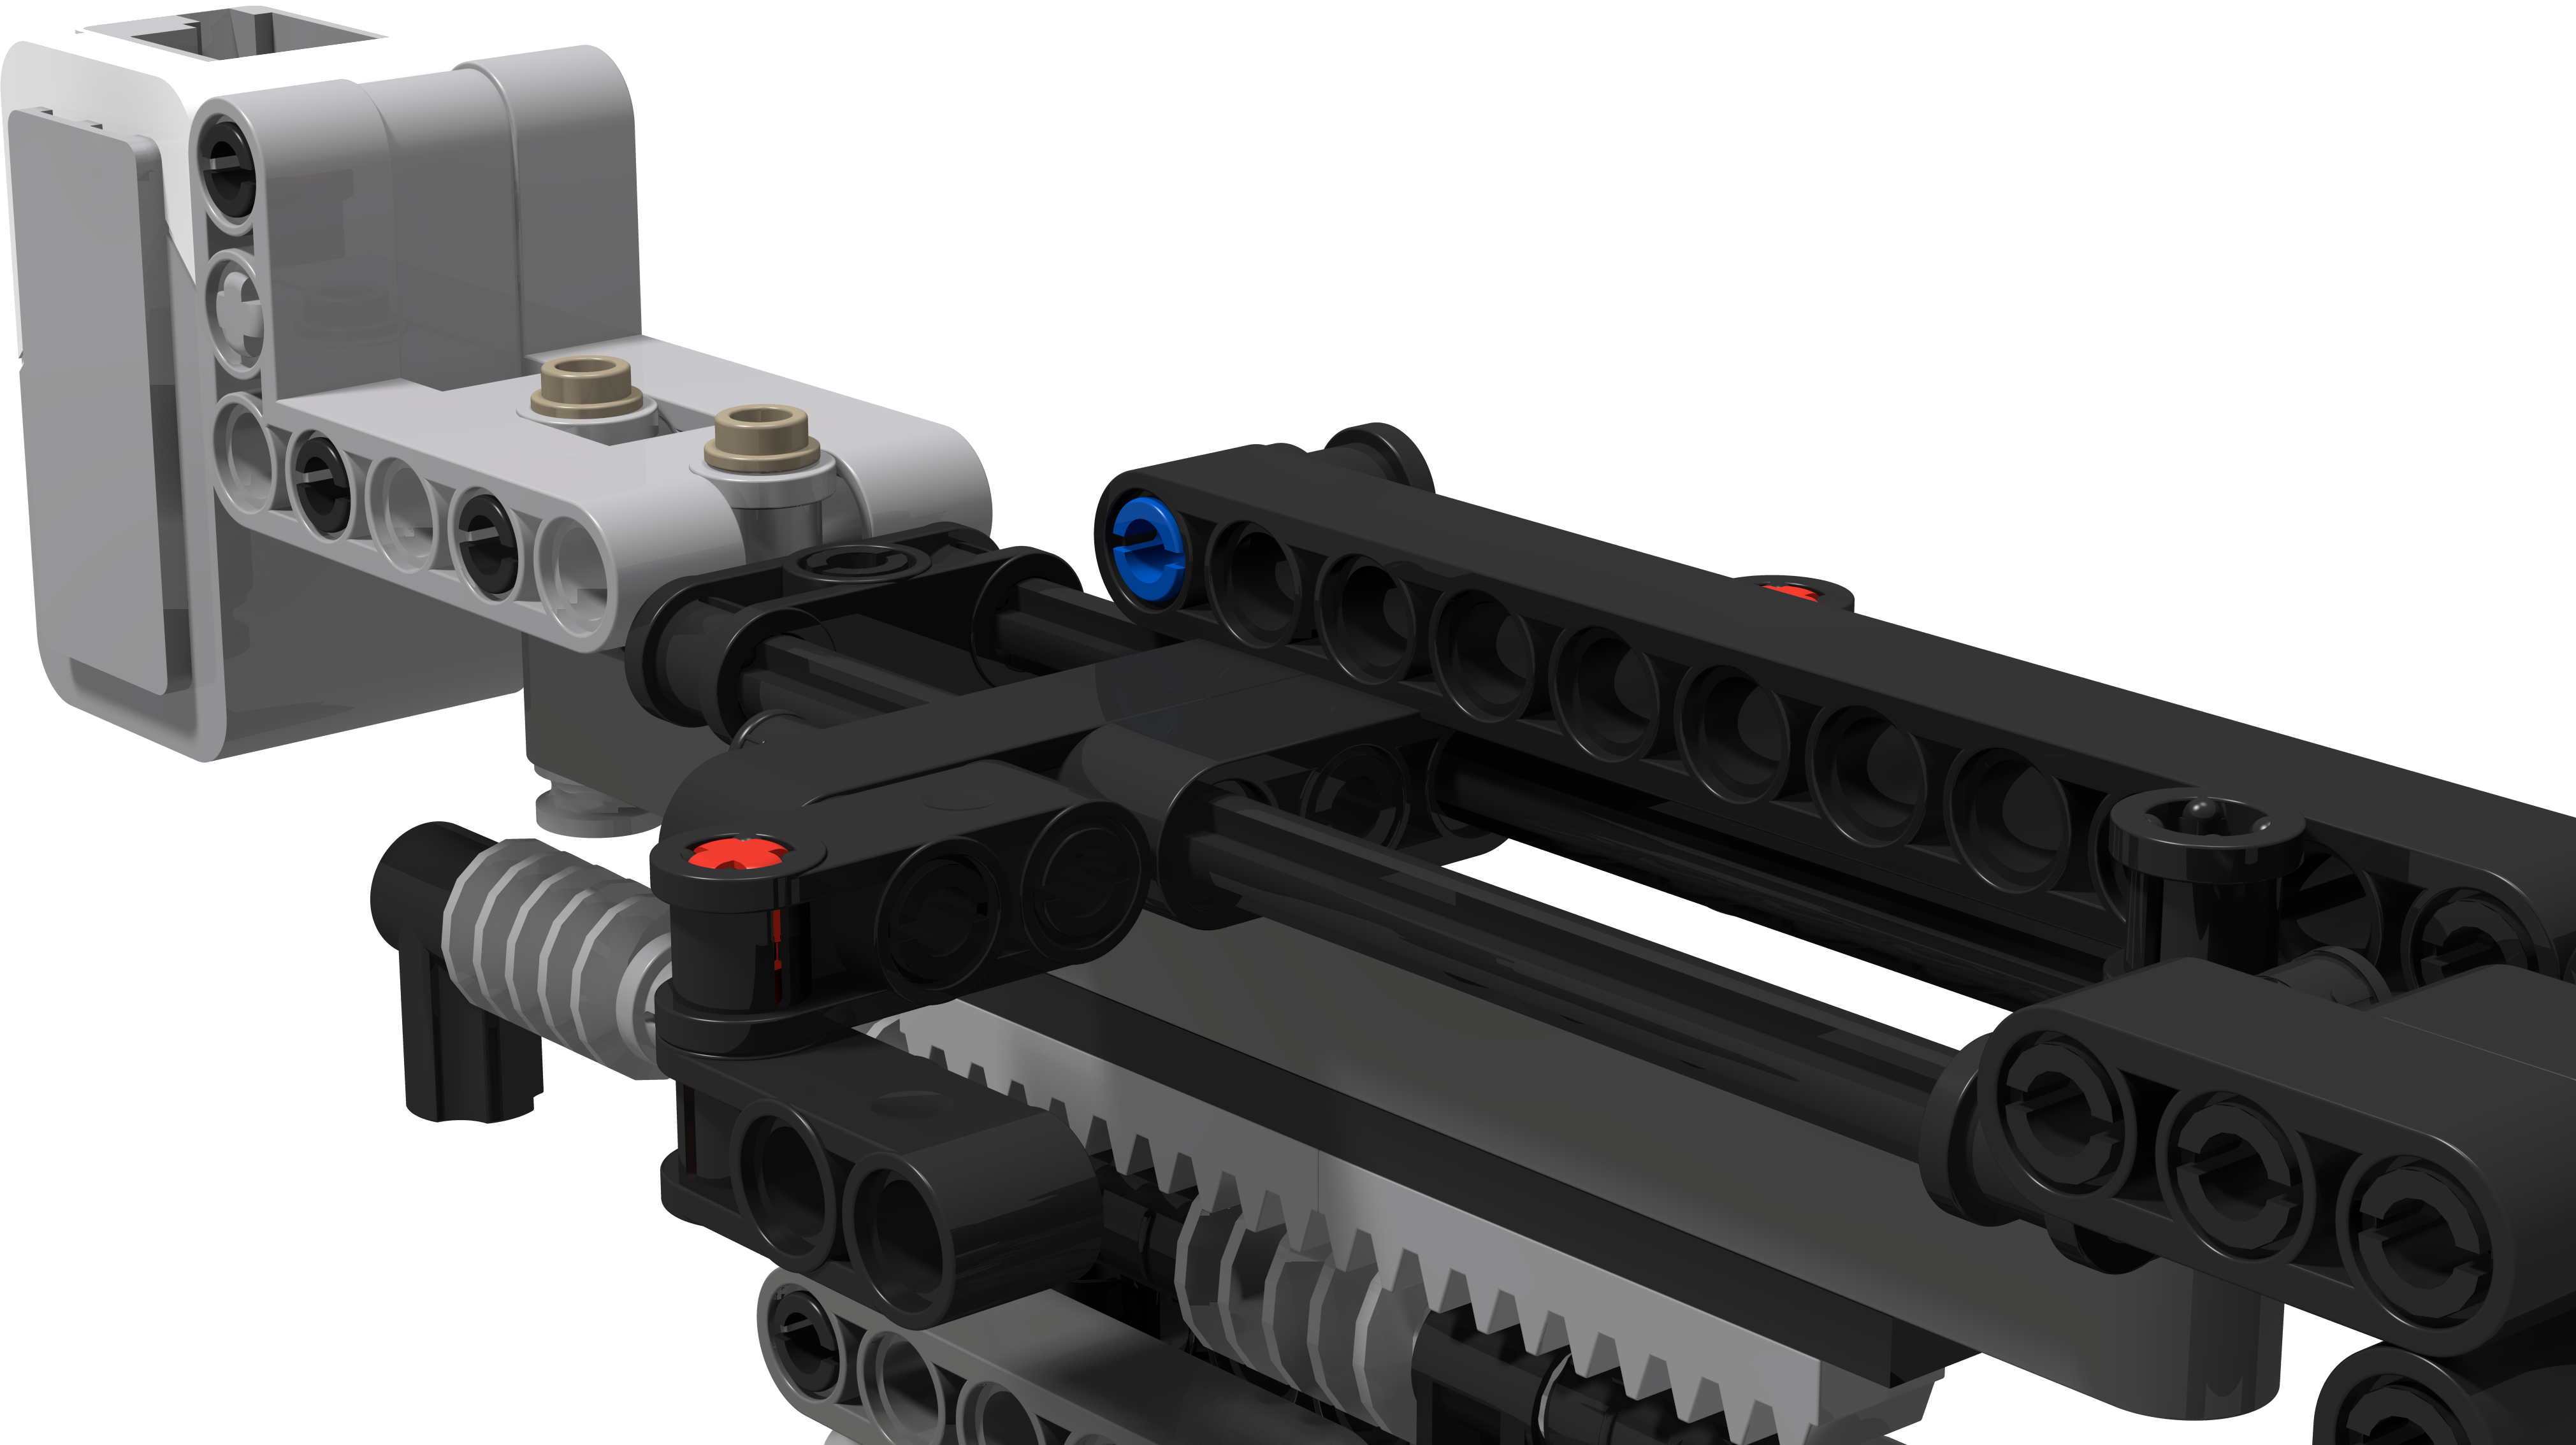
\includegraphics[width=\textwidth]{Resources/Images/rdrColorSensorShaftDetail.png}
			\caption{The assembly's mounting structure}
			\label{fig:rdrColorSensorShaftDetail}
		\end{subfigure}
		\caption{The colour sensor assembly}
		\label{fig:rdrColorSensor}
	\end{figure}
	
	Where the motors used for the cradle and the \move{x} arm can both rotate indefinitely without issue (colliding with other parts, for instance), the colour sensor motor cannot rotate indefinitely due to the limited freedom of the colour sensor assembly. When the assembly reaches the end of its travel, it will be stopped by the liftarm that holds the shafts, which will provide a level of resistance to the motor that could either damage the motor or force the MkI to break apart. For this reason, the 24-tooth gear \legopiece{60c01} (which is the first in the gear train) is a special type of \enquote{clutch gear}, shown in Figure \ref{fig:imgClutchGear}. This means that it will only transmit a maximum torque value of between 0.025 \si{\newton\metre} and 0.05 \si{\newton\metre}. The theoretical output torque of the gear train is 0.022 \si{\newton\metre}, so the clutch gear will function as a regular gear for the duration of colour sensor movement. When the assembly reaches its limit, the resistance to the gear train will cause the clutch gear to slip and the motor can continue turning without damaging itself or the MkI. 
	
	\begin{figure}[H]
		\centering
		\begin{minipage}{0.4\textwidth}
			\centering
			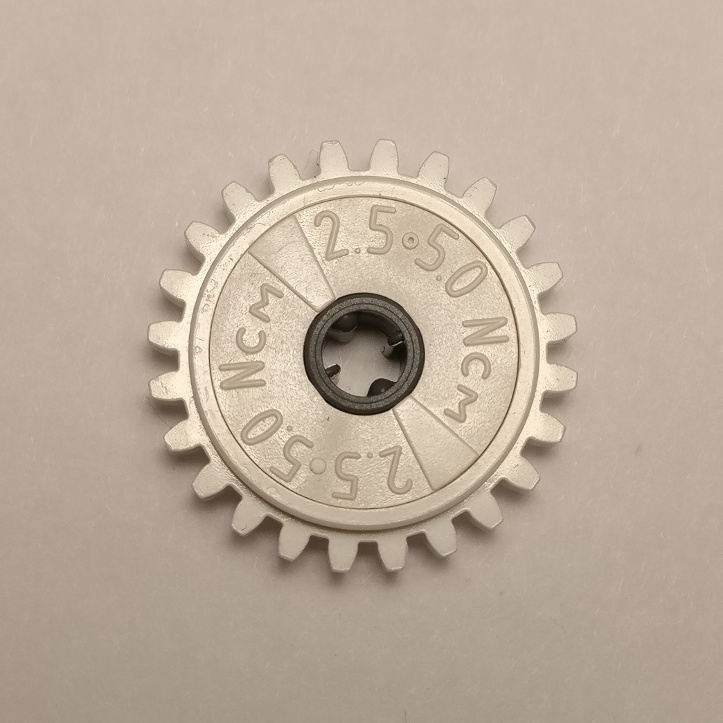
\includegraphics[width=0.8\textwidth]{Resources/Images/imgClutchGear.jpg}
			\caption{The clutch gear used to protect the motor}
			\label{fig:imgClutchGear}
		\end{minipage}%
		\hspace{10mm}
		\begin{minipage}{0.4\textwidth}
			\centering
			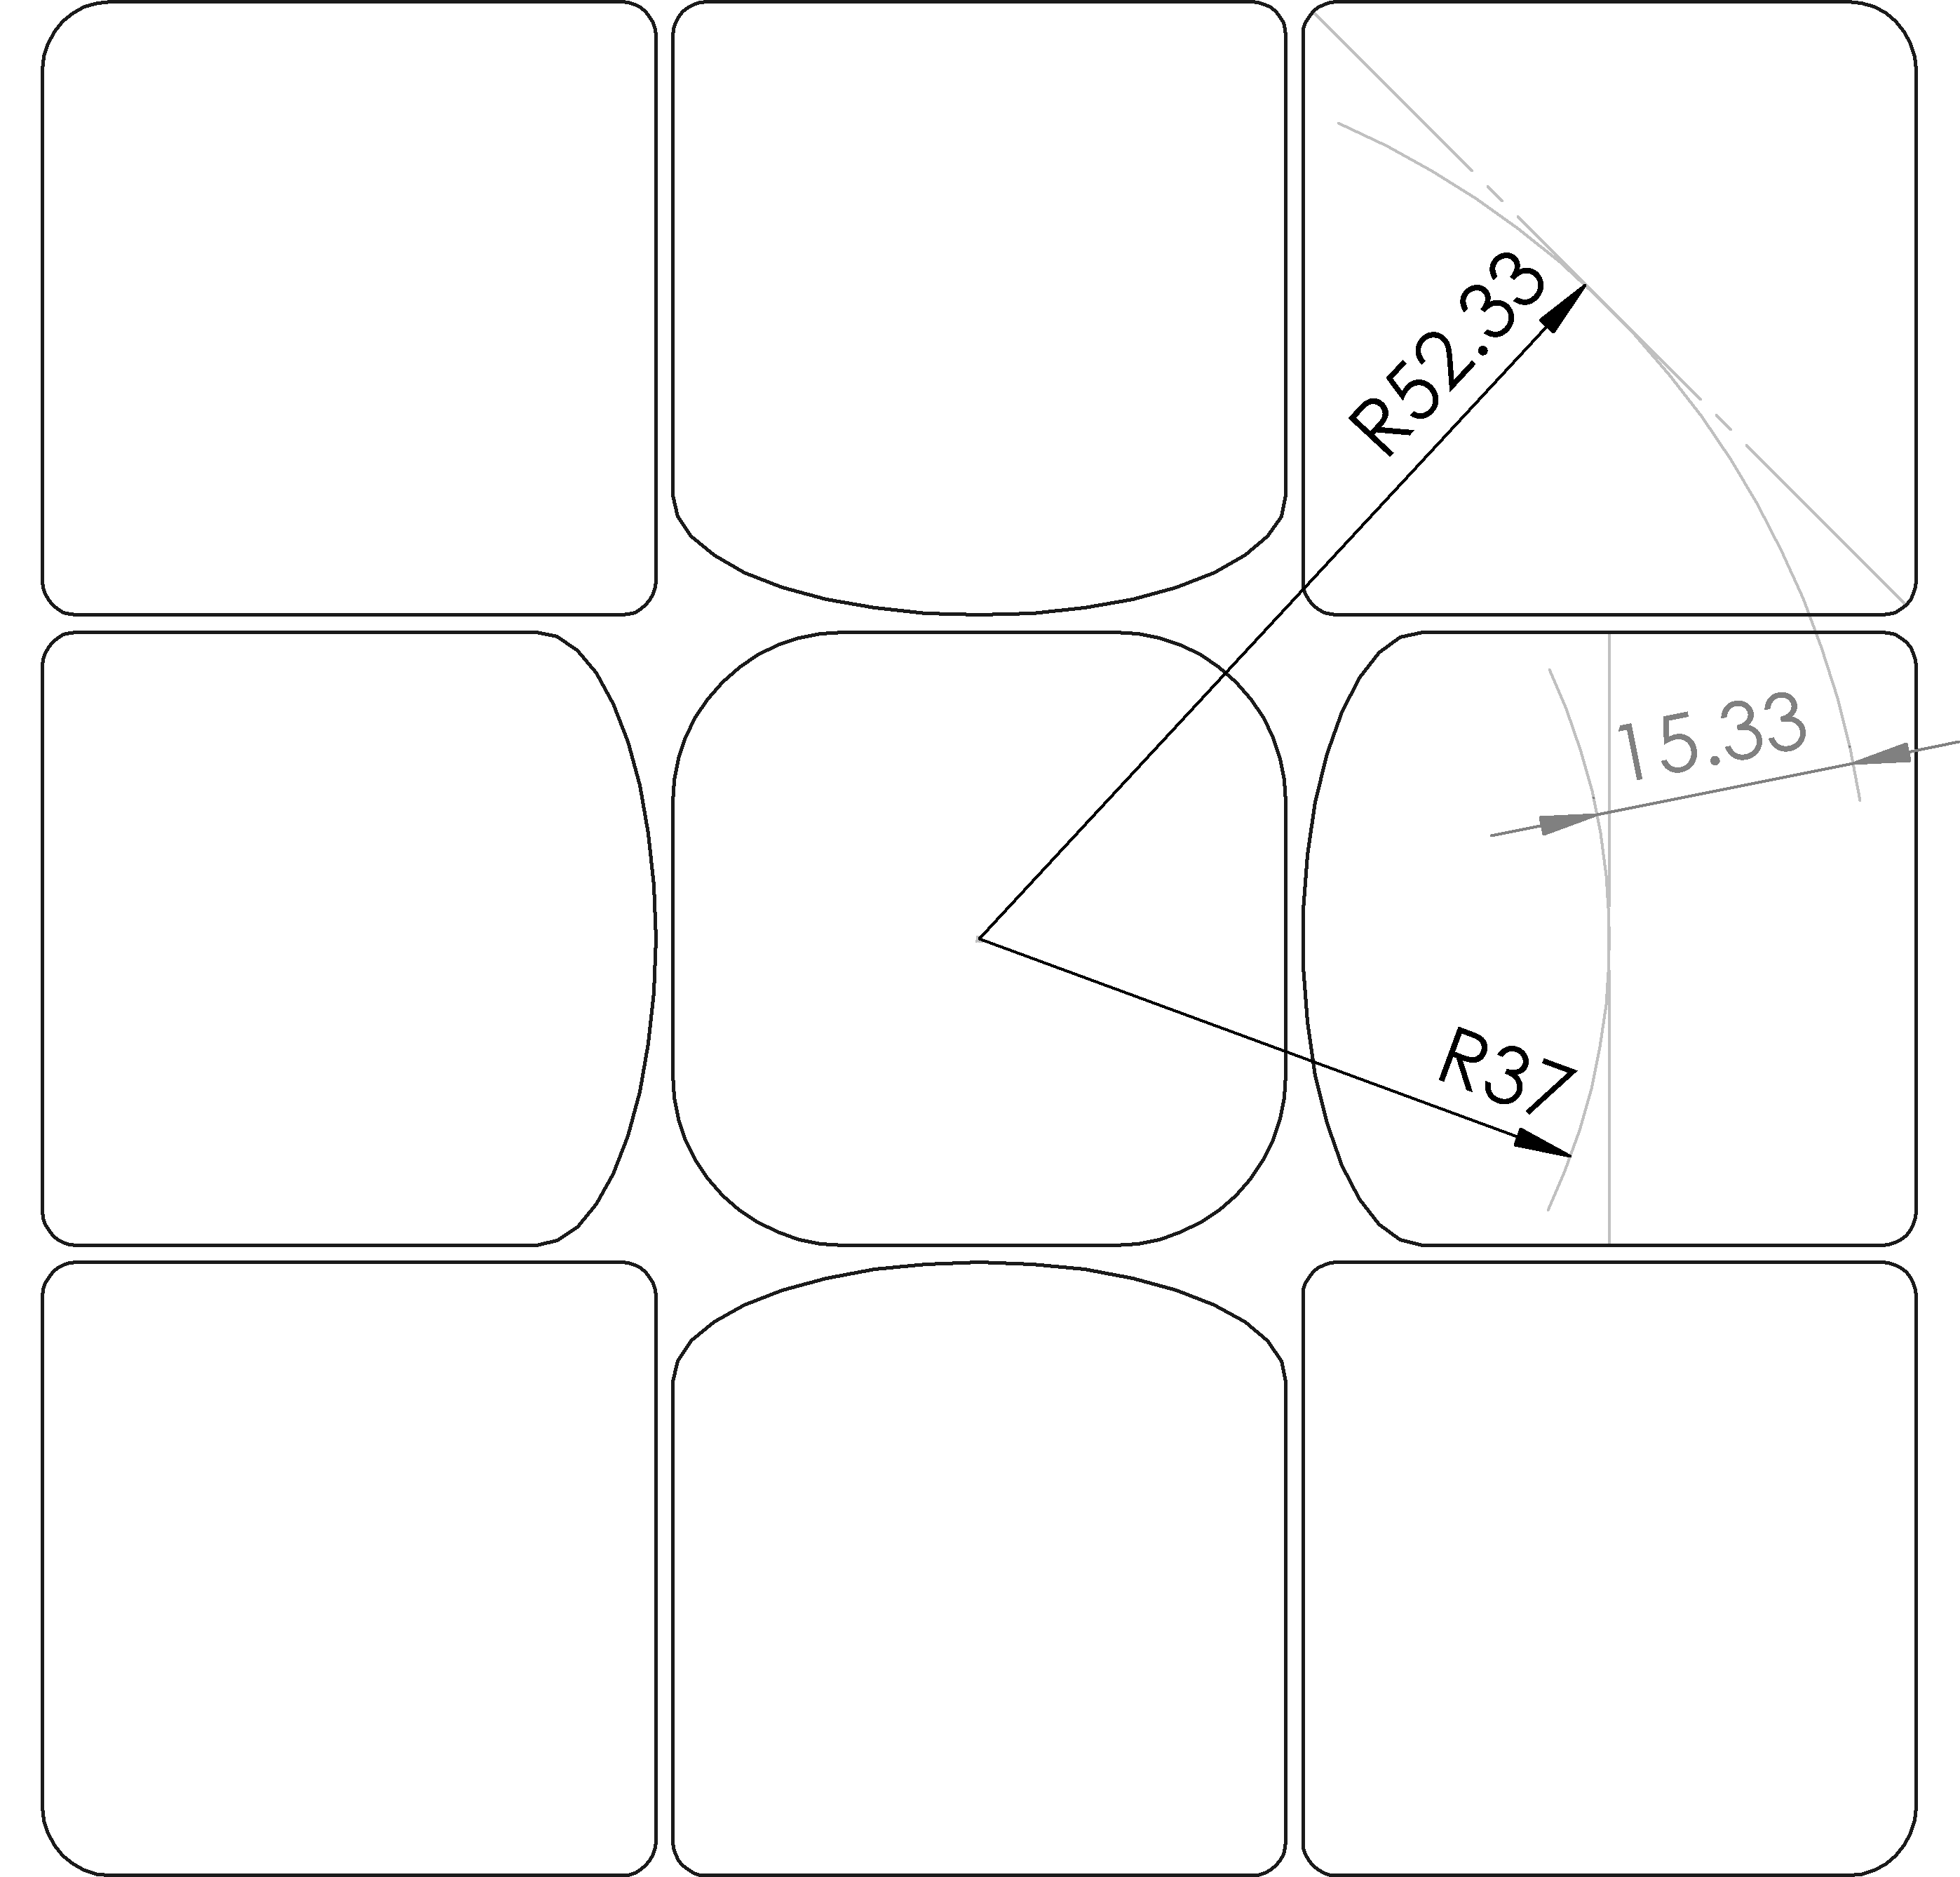
\includegraphics[width=0.8\textwidth]{Resources/Images/dwgCubeProfileCentreArcs.png}
			\caption{The measurements used in calculating the time for the colour sensor's movements}
			\label{fig:dwgCubeProfileCentreArcs}
		\end{minipage}
	\end{figure}
	
	\subsubsection{Algorithm Design}

	In order to scan a full Cube, the sequence \movesequence{X.X.X.Y.X.X.X} will be followed, and the \face{u} scanned every time a new face is seen, as shown by algorithms \ref{alg:scanupface} and \ref{alg:scancube} in Appendix \autoref{chp:appendixAlgorithms}.
	
	Algorithm \ref{alg:scanupface} is called once per face, and scans each facelet in turn. The function \lstinline|move_color_sensor| takes a single parameter: the stopping point for the motor, and there are three constants which are used as these stopping points. The motor is rotated until the tachometer value is greater-than-or-equal to the variable - or less-than if it is rotating backwards - so that if it is rotating faster than one \enquote{tacho-unit} at a time, it will not skip the stopping constant and continue indefinitely.
	
	Similarly to \lstinline|move_color_sensor|, \lstinline|rotate_cradle| takes a single parameter, the value which the current position of the motor is to be incremented by, in degrees. This value will then be multiplied as necessary to account for the gear train ratio.

	\subsection{Full Model}
	
	Figure \ref{fig:rdrFullRobotV1} demonstrates the full assembly of the MkI, including the main EV3 control brick. This model is the final result after any modifications made during the building process. As a result of the in-depth design process and any minor modifications, the MkI was optimised as much as possible with regards to functionality, structural integrity, and efficiency to work under restrictions from piece availability.
	
	\begin{figure}[H]
		\centering
		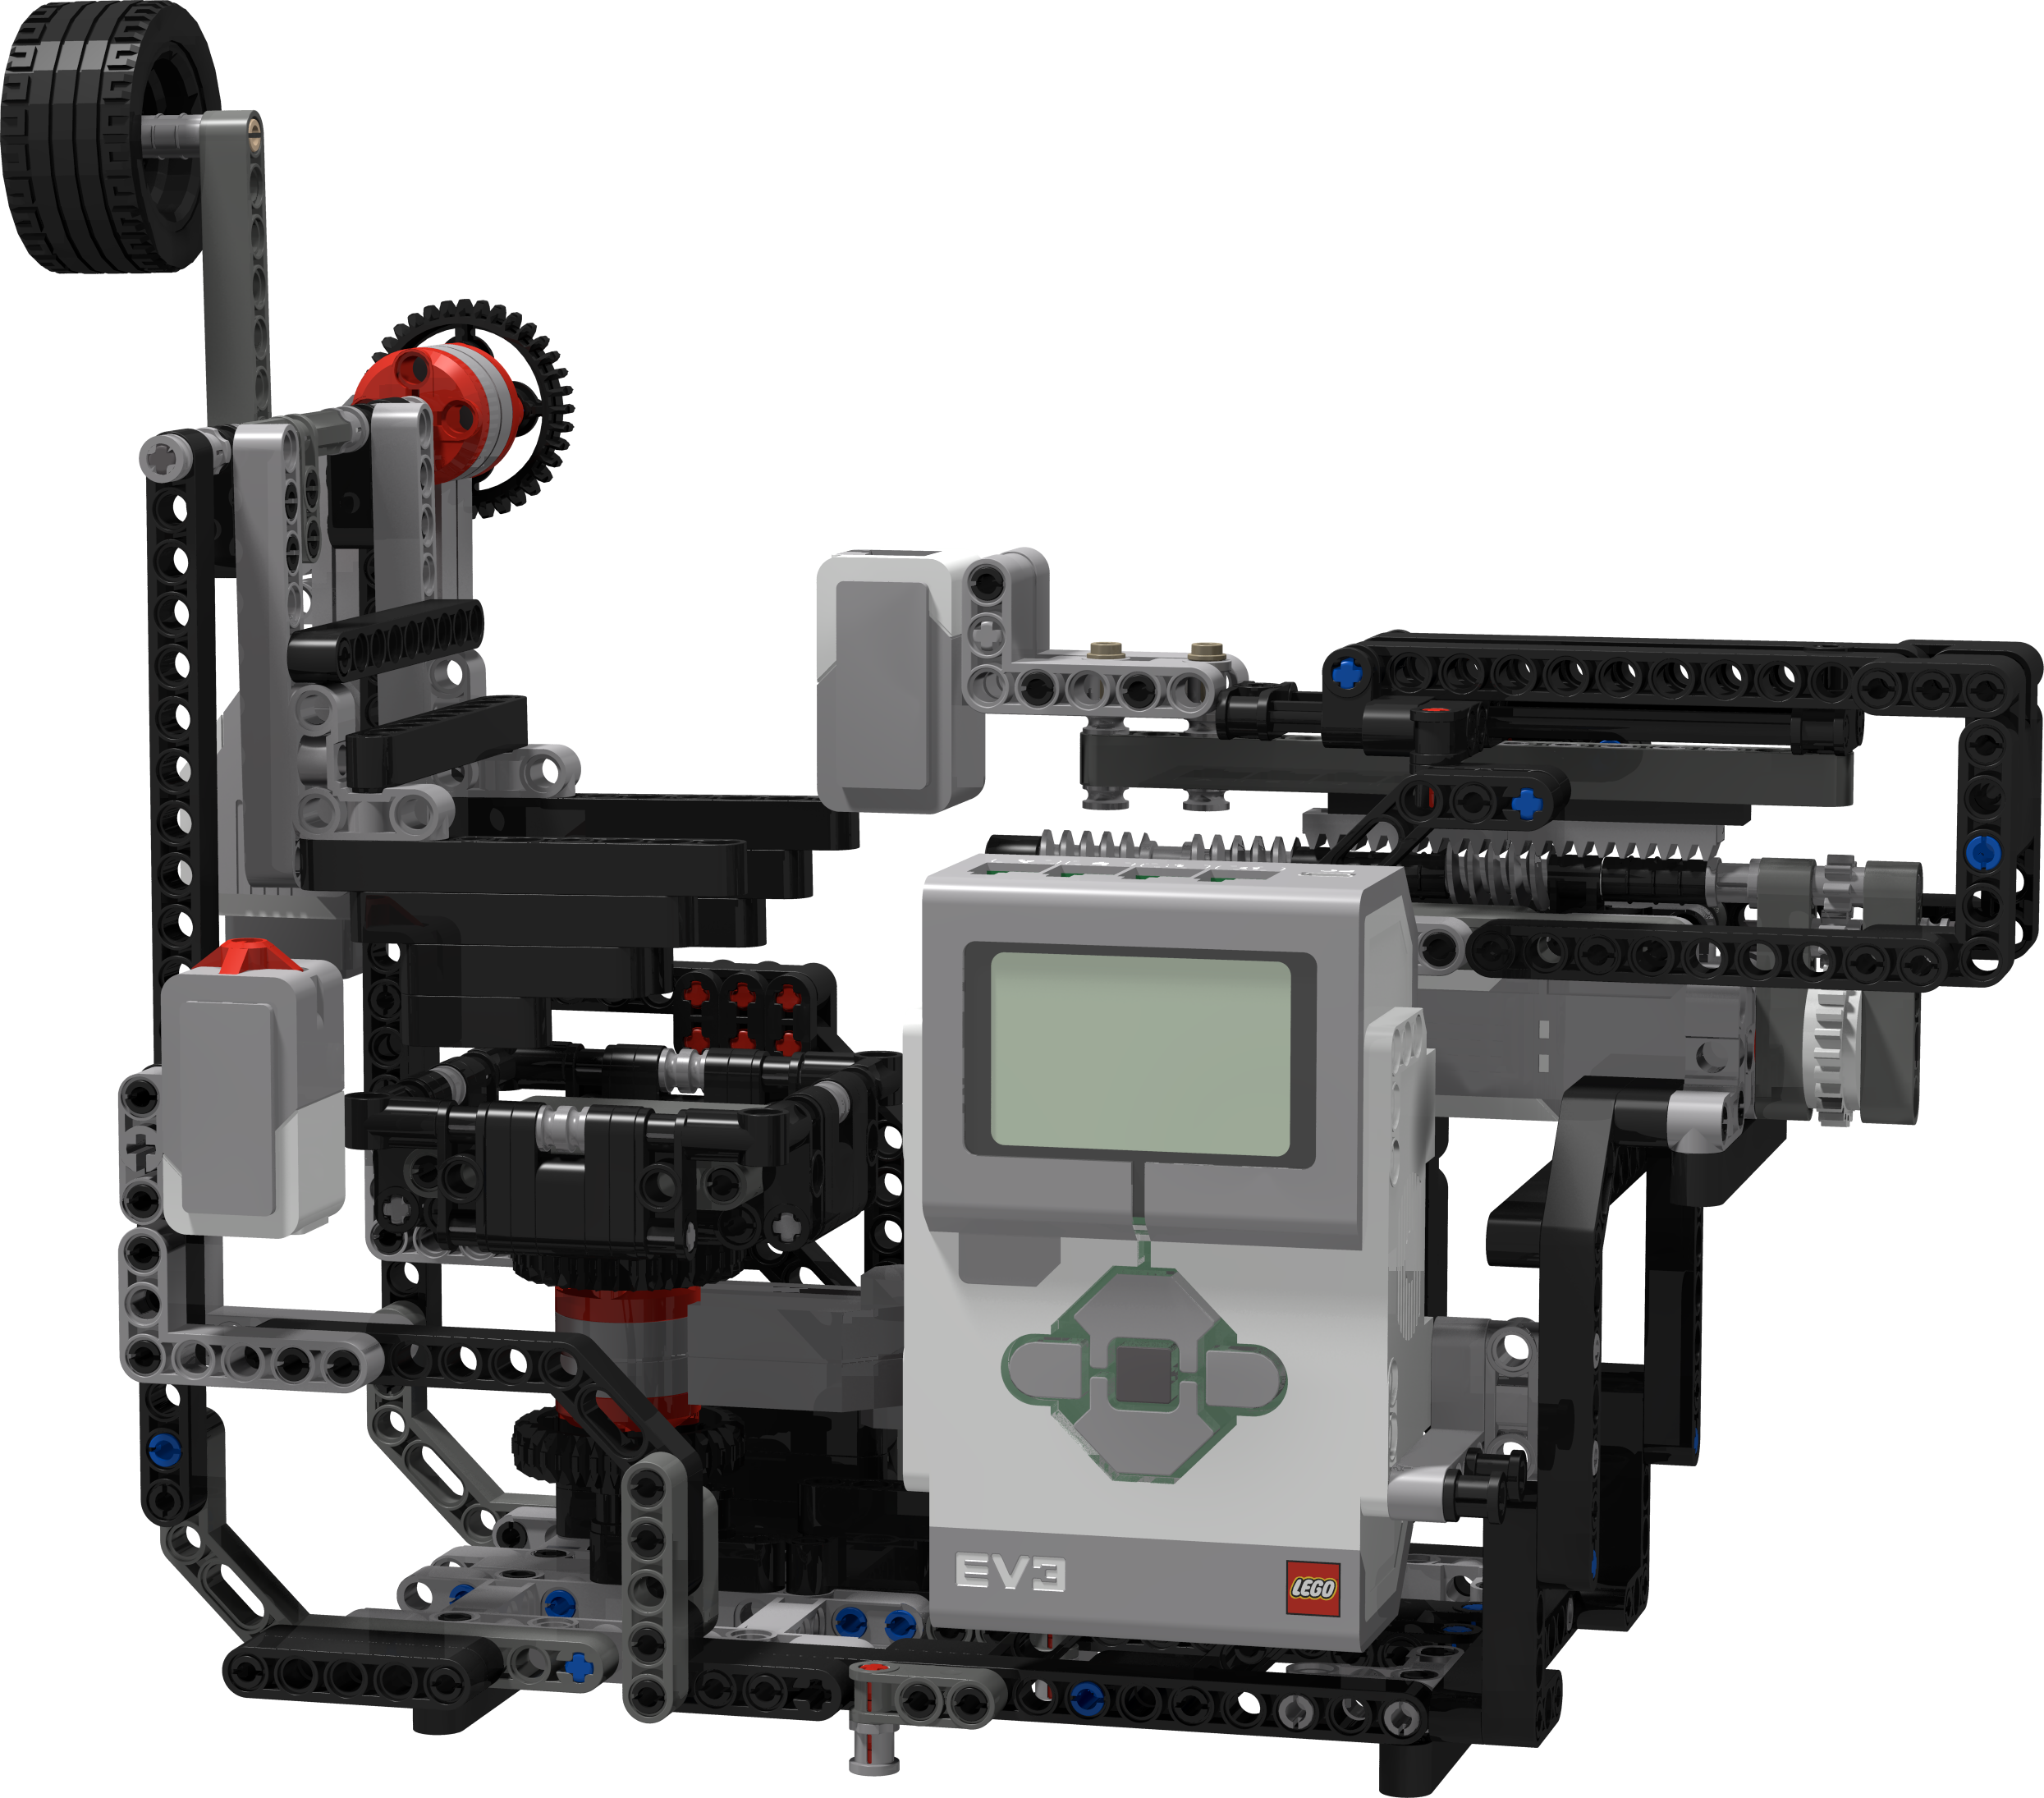
\includegraphics[width=0.6\textwidth]{Resources/Images/rdrFullRobotV1.png}
		\caption{The full robot assembly}
		\label{fig:rdrFullRobotV1}
	\end{figure}
	
	The build of the MkI is quite compact, and the design is largely influenced by the pieces available: during the modelling process, small sections were built to ensure functionality translated from the virtual model to the physical model as intended. Due to the limited quantity of \lego pieces, some less-than-optimal sections arose where two parts had to be connected but the necessary pieces were unavailable. This is visible behind the cradle, where six small red pieces \legopiece{32062} are used to connect two right-angled liftarms \legopiece{32009}. Another example of \enquote{design by necessity} is in the colour sensor's gear train: one medium \legopiece{60c01} and two small gears \legopiece{3647} were used consecutively instead of two medium, or one large and one small. The functional impact of some of these sections is negligible thanks to workarounds and extra pieces, however the aesthetics have unfortunately suffered minor setbacks in places.
	
	A touch sensor \legopiece{45507} is mounted on the side of the frame that surrounds the cradle and the \move{x} Arm. This adds the ability for user input when the software is running, without needing to access the operating system through the control brick. Simple tasks can be bound to the button at each stage of the solver (e.g. pause the scanning process if a move fails or confirm initialisation). The EV3 control brick is mounted on the side of the MkI to allow easy access to the controls which allow navigation of the file system and turning the brick on and off. It is held in place by several long pins \legopiece{32054} which can be easily retracted to allow quick removal of the brick so the batteries can be changed.

	\subsection{Implementation and Testing}
	
	The MkI was built according to the design specifications laid out above, with little to no modification throughout. To thoroughly test the functions of the MkI (and any subsequent designs), a simple trial was designed to repeatedly test and optimise the motorised functions of the MkI.
	
	The first part of each trial was to run the scanning process from start to end, as described by algorithms \ref{alg:scanupface} and \ref{alg:scancube}, to test the movement of all three fundamental components. Optimisations were made between each trial, such as refining the constants used for setting the stopping points for the components. Further optimisations involved modifying the MkI design to reinforce the framework, or altering the rotational velocity of the motors amongst other changes. The second part of the trial runs a thorough move sequence to check all move combinations function as expected. This covers the accuracy of the cradle for \move{d}s and \move{y}s, the accuracy and the effectiveness of the \move{x} arm's guards, and the success of the \move{x}s.
	
	\subsubsection{Major Issues} \label{sec:mkIMajorIssues}
	
	The first major issue with the functionality of the MkI was actually software-based - however it is discussed here because it produced a hardware issue which affected the MkI's design. The details of the code used are discussed in section \ref{sec:robotObject}. In the test runs described above, the pass condition was a manual comparison between the virtual Cube and the real-world Cube, where the position of the Cube was checked against an on-screen printout. The colour sensor has different modes to read colours: \lstinline|COL_COLOR|, which returns an integer between zero and seven (inclusive) to represent a specific colour; \lstinline|RGB_RAW|, which returns the RGB values read by the sensor; and other modes which read light intensity rather than the colour. For this application, the \lstinline|COL_COLOR| is the most suitable mode because it will not require the RGB values to be parsed into one of the six colours.
	
	Unfortunately, the on-screen printout was always a mix of blue, red and white rather than the expected mix of the usual six colours. To properly debug this problem, the mode was set to \lstinline|RGB_RAW| and the RGB values returned by the colour sensor were compared with values read by the camera on a OnePlus 3\footnote{A simple RGB colour picking application was used \cite{RangoApps2015}}.
	
   	\begin{table}[H]
		\def\arraystretch{1.25}
		\centering
		\caption{The colour values returned by a OnePlus 3 and the \lego Colour Sensor}
		\label{tab:coloursensor1}
		\begin{tabular}{M{0.1\textwidth}M{0.075\textwidth}M{0.075\textwidth}M{0.075\textwidth}M{0.07\textwidth}M{0.075\textwidth}M{0.075\textwidth}M{0.075\textwidth}M{0.07\textwidth}}
			\toprule
			\multirow{2}{*}{\tbo{Face}} & \multicolumn{4}{c}{\tbo{OnePlus 3}} 			& \multicolumn{4}{c}{\tbo{\lego Colour Sensor}}  \\
										& \tbo{Red}&\tbo{Green}&\tbo{Blue}&\tbo{RGB}	& \tbo{Red}&\tbo{Green}&\tbo{Blue}&\tbo{RGB} 	\\
			\midrule
			White	&229&224&221&\cellcolor[rgb]{0.90,0.88,0.87}	&79&106&53&\cellcolor[rgb]{0.31,0.42,0.21}\textcolor{white}{White}	\\	
			Yellow	&181&195&0  &\cellcolor[rgb]{0.71,0.76,0.00}	&73&97 &76&\cellcolor[rgb]{0.29,0.38,0.30}\textcolor{white}{White}	\\
			Red		&223&25 &35 &\cellcolor[rgb]{0.87,0.10,0.14}	&52&24 &9 &\cellcolor[rgb]{0.20,0.09,0.04}\textcolor{white}{Red}	\\
			Orange	&251&127&21 &\cellcolor[rgb]{0.98,0.50,0.08}	&68&93 &75&\cellcolor[rgb]{0.27,0.36,0.29}\textcolor{white}{White}	\\
			Green	&34 &186&8  &\cellcolor[rgb]{0.13,0.73,0.03}	&25&71 &48&\cellcolor[rgb]{0.10,0.28,0.19}\textcolor{white}{Blue}	\\
			Blue	&0  &130&255&\cellcolor[rgb]{0.00,0.51,1.00}	&10&31 &31&\cellcolor[rgb]{0.04,0.12,0.12}\textcolor{white}{Blue}	\\
			\bottomrule
		\end{tabular}
	\end{table}

	Table \ref{tab:coloursensor1} compares the values read by both devices, along with the RGB values. The \lstinline|COL_COLOR| values have been overlaid on the colours returned by the \lego sensor to show how they are interpreted by ev3dev. After many more tests, it became apparent that the issue was that the colour sensor cannot detect fluorescent colours - which is the Valk 3's colour scheme.
	
	The solution to this problem was to print sensor-readable colours on standard white sticky labels and apply them over the stickers which were being incorrectly read (the yellow, green and orange sides). The end result is visible in Figure \ref{fig:imgCubeStickersComparison}, next to a non-stickered Valk 3. The orange side has been replaced with brown stickers because the colour sensor reads the five other colours, and then brown - not orange. For this project however, the colour will be referred to as orange for consistency.

	\begin{figure}[H]
		\centering
		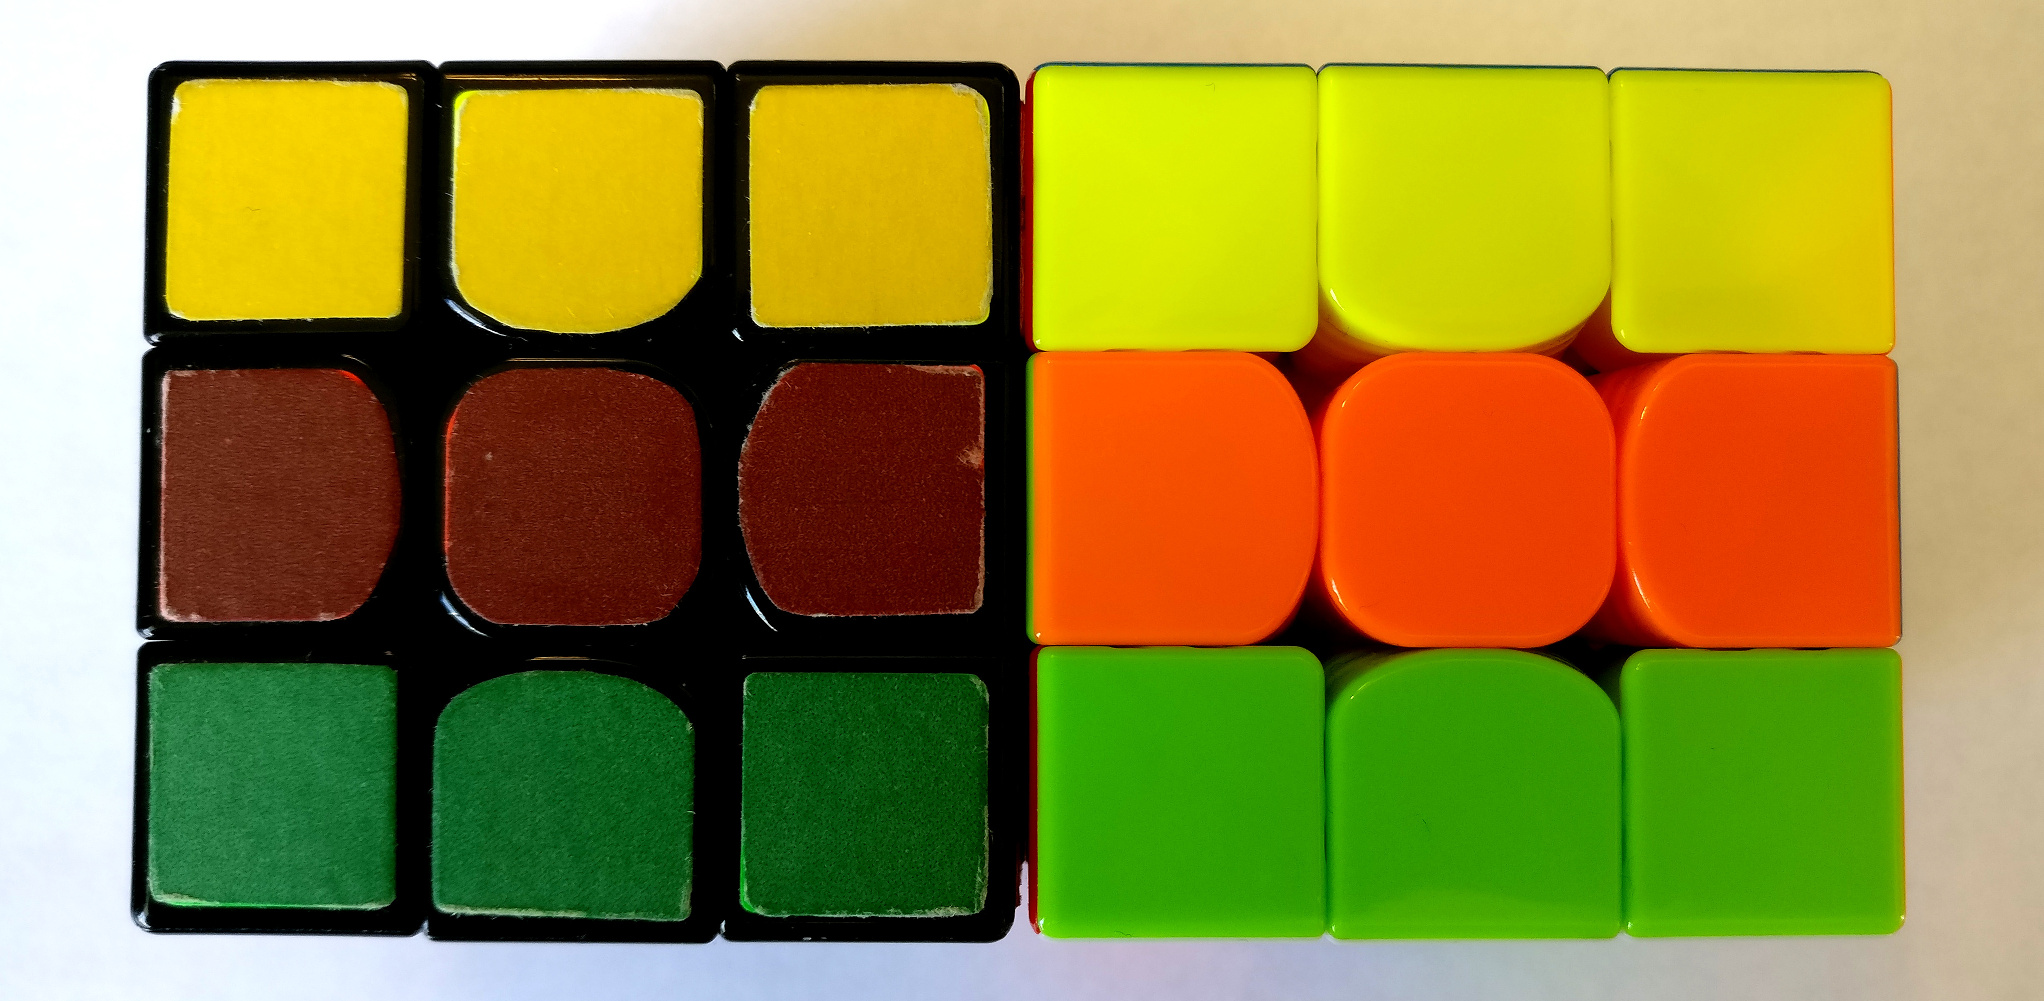
\includegraphics[width=0.5\textwidth]{Resources/Images/imgCubeStickersComparison.jpg}
		\caption{Side-by-side comparison of the Valk 3 with and without stickers}
		\label{fig:imgCubeStickersComparison}
	\end{figure}

	Table \ref{tab:coloursensor2} shows that the new stickers greatly improved the accuracy of the colour sensor's readings. Although the colours in the final column of the table are all very dark and almost indistinguishable, the colour sensor has no difficulty in telling the colours apart. As such, the sensor's accuracy with the new stickers is sufficient for this project.
	
   	\begin{table}[H]
		\def\arraystretch{1.25}
		\centering
		\caption{A comparison of the colour values returned before and after the application of coloured stickers}
		\label{tab:coloursensor2}
		\begin{tabular}{M{0.1\textwidth}M{0.075\textwidth}M{0.075\textwidth}M{0.075\textwidth}M{0.07\textwidth}M{0.075\textwidth}M{0.075\textwidth}M{0.075\textwidth}M{0.07\textwidth}}
			\toprule
			\multirow{2}{*}{\tbo{Face}} & \multicolumn{4}{c}{\tbo{Original Stickers}} 			& \multicolumn{4}{c}{\tbo{Modified Stickers}}  \\
			& \tbo{Red}&\tbo{Green}&\tbo{Blue}&\tbo{RGB}	& \tbo{Red}&\tbo{Green}&\tbo{Blue}&\tbo{RGB} 	\\
			\midrule
			White	&79&106&53&\cellcolor[rgb]{0.31,0.42,0.21}\textcolor{white}{White}	&75&101&51&\cellcolor[rgb]{0.29,0.40,0.20}\textcolor{white}{White}	\\
			Yellow	&73&97 &76&\cellcolor[rgb]{0.29,0.38,0.30}\textcolor{white}{White}	&58&46 &8 &\cellcolor[rgb]{0.23,0.18,0.03}\textcolor{white}{Yellow}	\\
			Red		&52&24 &9 &\cellcolor[rgb]{0.20,0.09,0.04}\textcolor{white}{Red}	&41&18 &5 &\cellcolor[rgb]{0.16,0.07,0.02}\textcolor{white}{Red}	\\
			Orange	&68&93 &75&\cellcolor[rgb]{0.27,0.36,0.29}\textcolor{white}{White}	&24&14 &5 &\cellcolor[rgb]{0.09,0.05,0.02}\textcolor{white}{Orange}	\\
			Green	&25&71 &48&\cellcolor[rgb]{0.10,0.28,0.19}\textcolor{white}{Blue}	&11&33 &7 &\cellcolor[rgb]{0.04,0.13,0.03}\textcolor{white}{Green}	\\
			Blue	&10&31 &31&\cellcolor[rgb]{0.04,0.12,0.12}\textcolor{white}{Blue}	&9 &24 &17&\cellcolor[rgb]{0.04,0.09,0.06}\textcolor{white}{Blue}	\\
			\bottomrule
		\end{tabular}
	\end{table}

	The addition of the stickers was a double-edged sword: the coefficient of friction between the Cube and the curved edge of the cradle wall was now too high for the Cube to slide back into the cradle. Rather than spending time redesigning the cradle or changing the arm design to pull the Cube back in, the easiest solution was simply to tilt the entire robot:
	
	\begin{figure}[H]
		\centering
		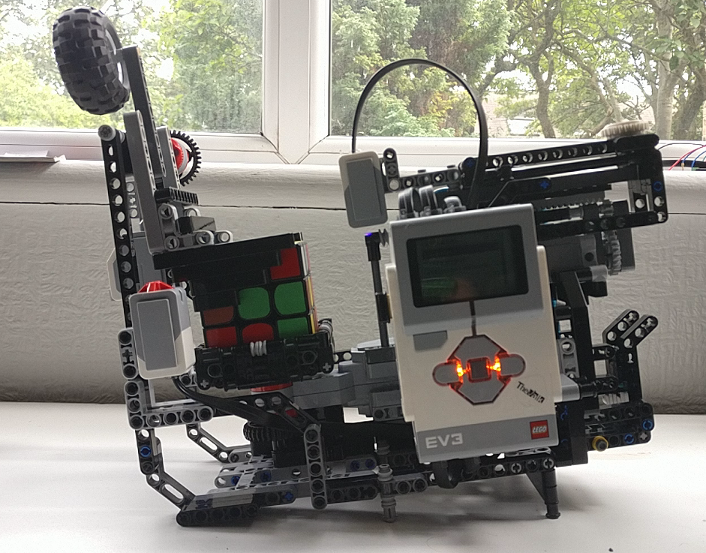
\includegraphics[width=0.5\textwidth]{Resources/Images/imgCubeSolverV1.png}
		\caption{The MkI had a distinctive tilt to ensure the success of \move{x}s}
		\label{fig:imgCubeSolverV1}
	\end{figure}

	The second major issue with the MkI was caused by the newly added tilt and the design of the \move{x} arm: when the arm pushed the Cube to start an \move{x}, the Cube would often fall out of the cradle instead of pivoting. There was no obvious solution to this problem, other than making the wheel larger to spread the force across the face of the Cube. However, a larger wheel meant that the arm became unbalanced and the strength of the arm was compromised. This led to the liftarm that held the wheel falling off the MkI mid-process more than once, as shown in Figure \ref{fig:mkIArmCollapse} (three frames extracted from a video of the scanning process).

	\begin{figure}[H]
		\centering
		\begin{subfigure}[b]{0.25\textwidth}
			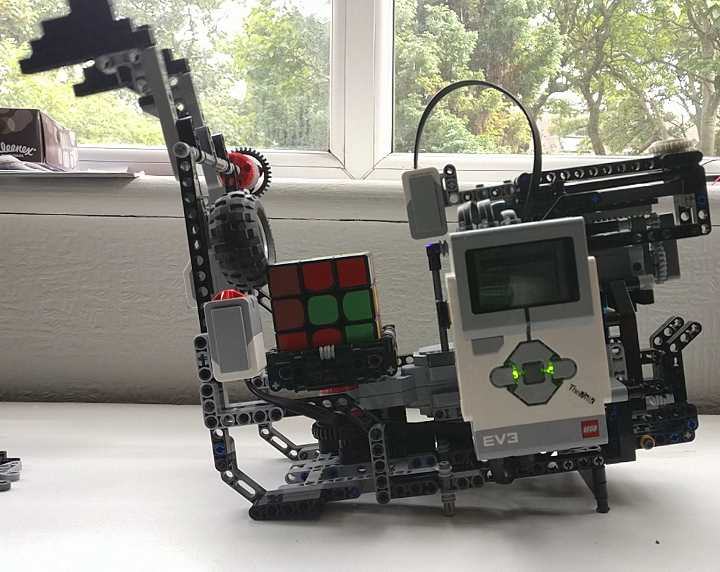
\includegraphics[width=\textwidth]{Resources/Images/imgMkIArmCollapse1.png}
		\end{subfigure}
		\hspace{5mm}
		\begin{subfigure}[b]{0.25\textwidth}
			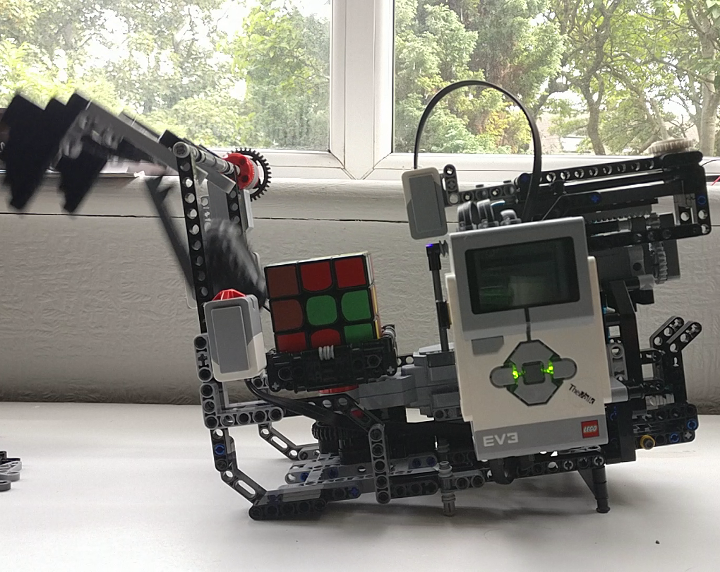
\includegraphics[width=\textwidth]{Resources/Images/imgMkIArmCollapse2.png}
		\end{subfigure}
		\hspace{5mm}
		\begin{subfigure}[b]{0.25\textwidth}
			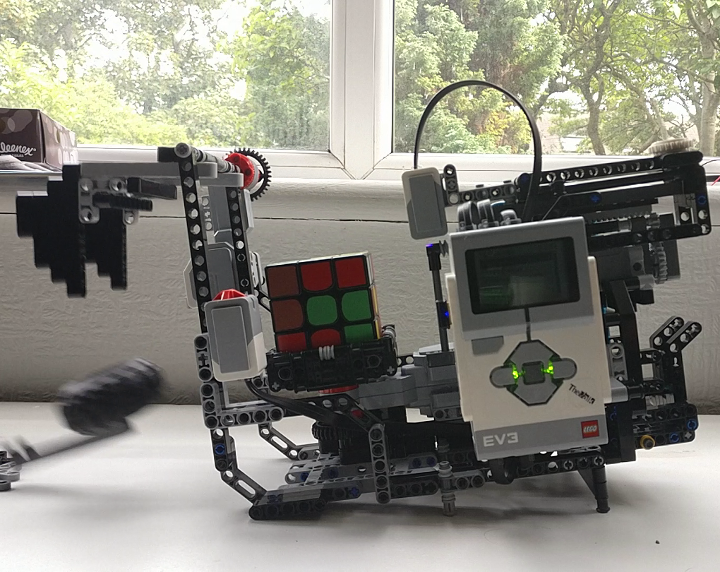
\includegraphics[width=\textwidth]{Resources/Images/imgMkIArmCollapse3.png}
		\end{subfigure}
		\caption{The MkI \move{x} arm broke under greater resistance}
		\label{fig:mkIArmCollapse}
	\end{figure}
	
	The final issue with the MkI, which prompted a complete rebuild, was an inherent issue with the large motor that rotated the cradle. As with all DC motors, there is a slight amount of \enquote{play} in the rotor: it has a few degrees of freedom either side of its current position. The play reduced the accuracy of the cradle, by effectively introducing a zero error for each rotation. A problem of this magnitude required a full analysis and re-design of the robot.

    \section{Robot Design MkII}
	\subsection{Improvements on MkI}
	Aside from the few major issues outlined above, the time spent testing and using the MkI led to the discovery of many more smaller issues that would be addressed during the design of the second iteration of the robot's design: the MkII. These minor issues are discussed below, as proof of the careful consideration used and to validate the choices made in designing the MkII.
	
	\subsubsection{Motor Initialisation}
	
	During the testing and general usage of the MkI, there were many occurrences of a fatal runtime error which would leave the motors out of their starting position. The usual cause of this was a \lstinline|StallError| from one of the motors or the voltage supply from the batteries becoming too low. The incorrect positioning required the motors to be initialised when restarting the program. To assist in this procedure, large gears \legopiece{32498} were added to the motors which allows them to be returned to their respective initial positions.
	
	\begin{figure}[H]
		\centering
		\begin{subfigure}[b]{0.25\textwidth}
			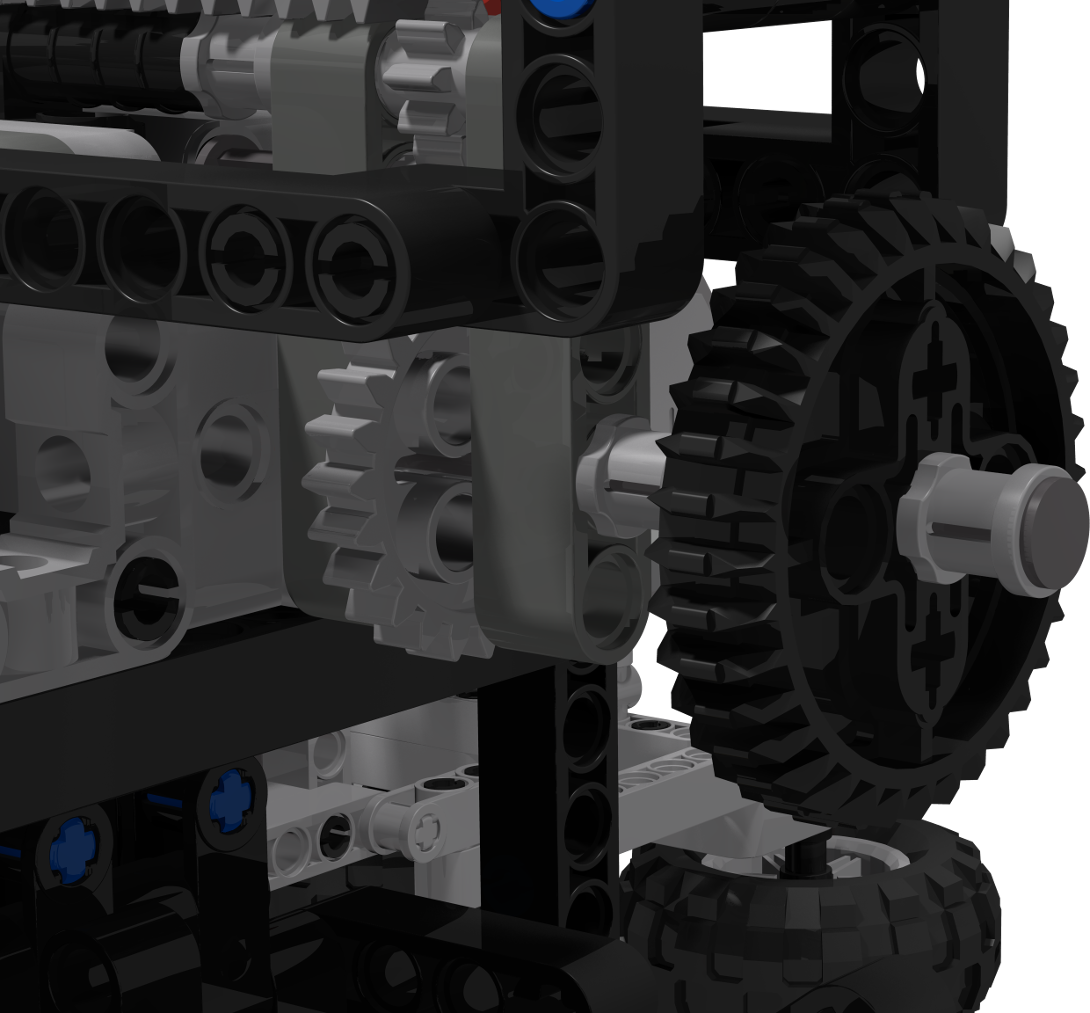
\includegraphics[width=\textwidth]{Resources/Images/rdrInitialiser1.png}
			\caption{Colour Sensor initialiser}
			\label{fig:rdrInitialiser1}
		\end{subfigure}
		\hspace{10mm}
		\begin{subfigure}[b]{0.25\textwidth}
			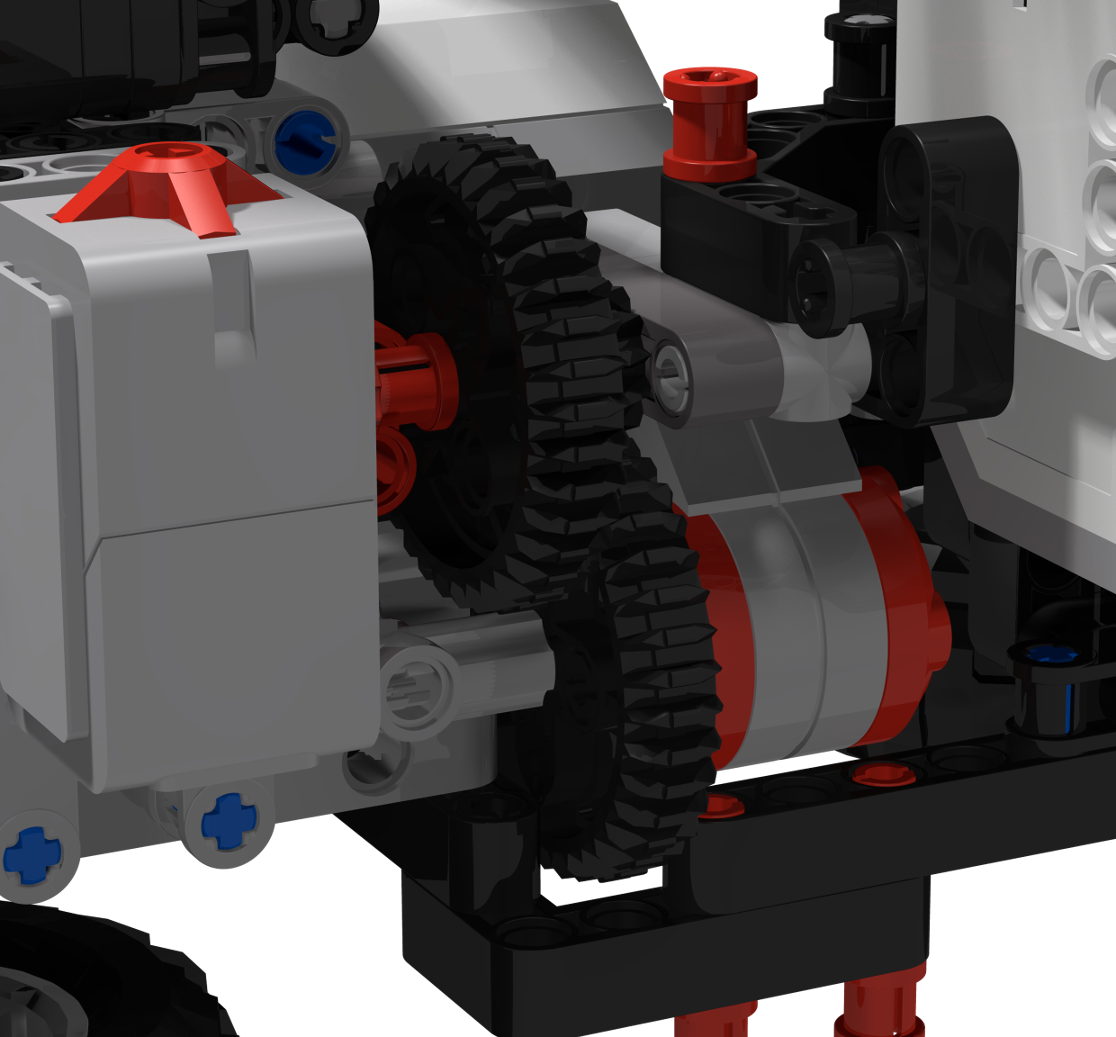
\includegraphics[width=\textwidth]{Resources/Images/rdrInitialiser2.png}
			\caption{Cradle initialiser}
			\label{fig:rdrInitialiser2}
		\end{subfigure}
		\hspace{10mm}
		\begin{subfigure}[b]{0.25\textwidth}
			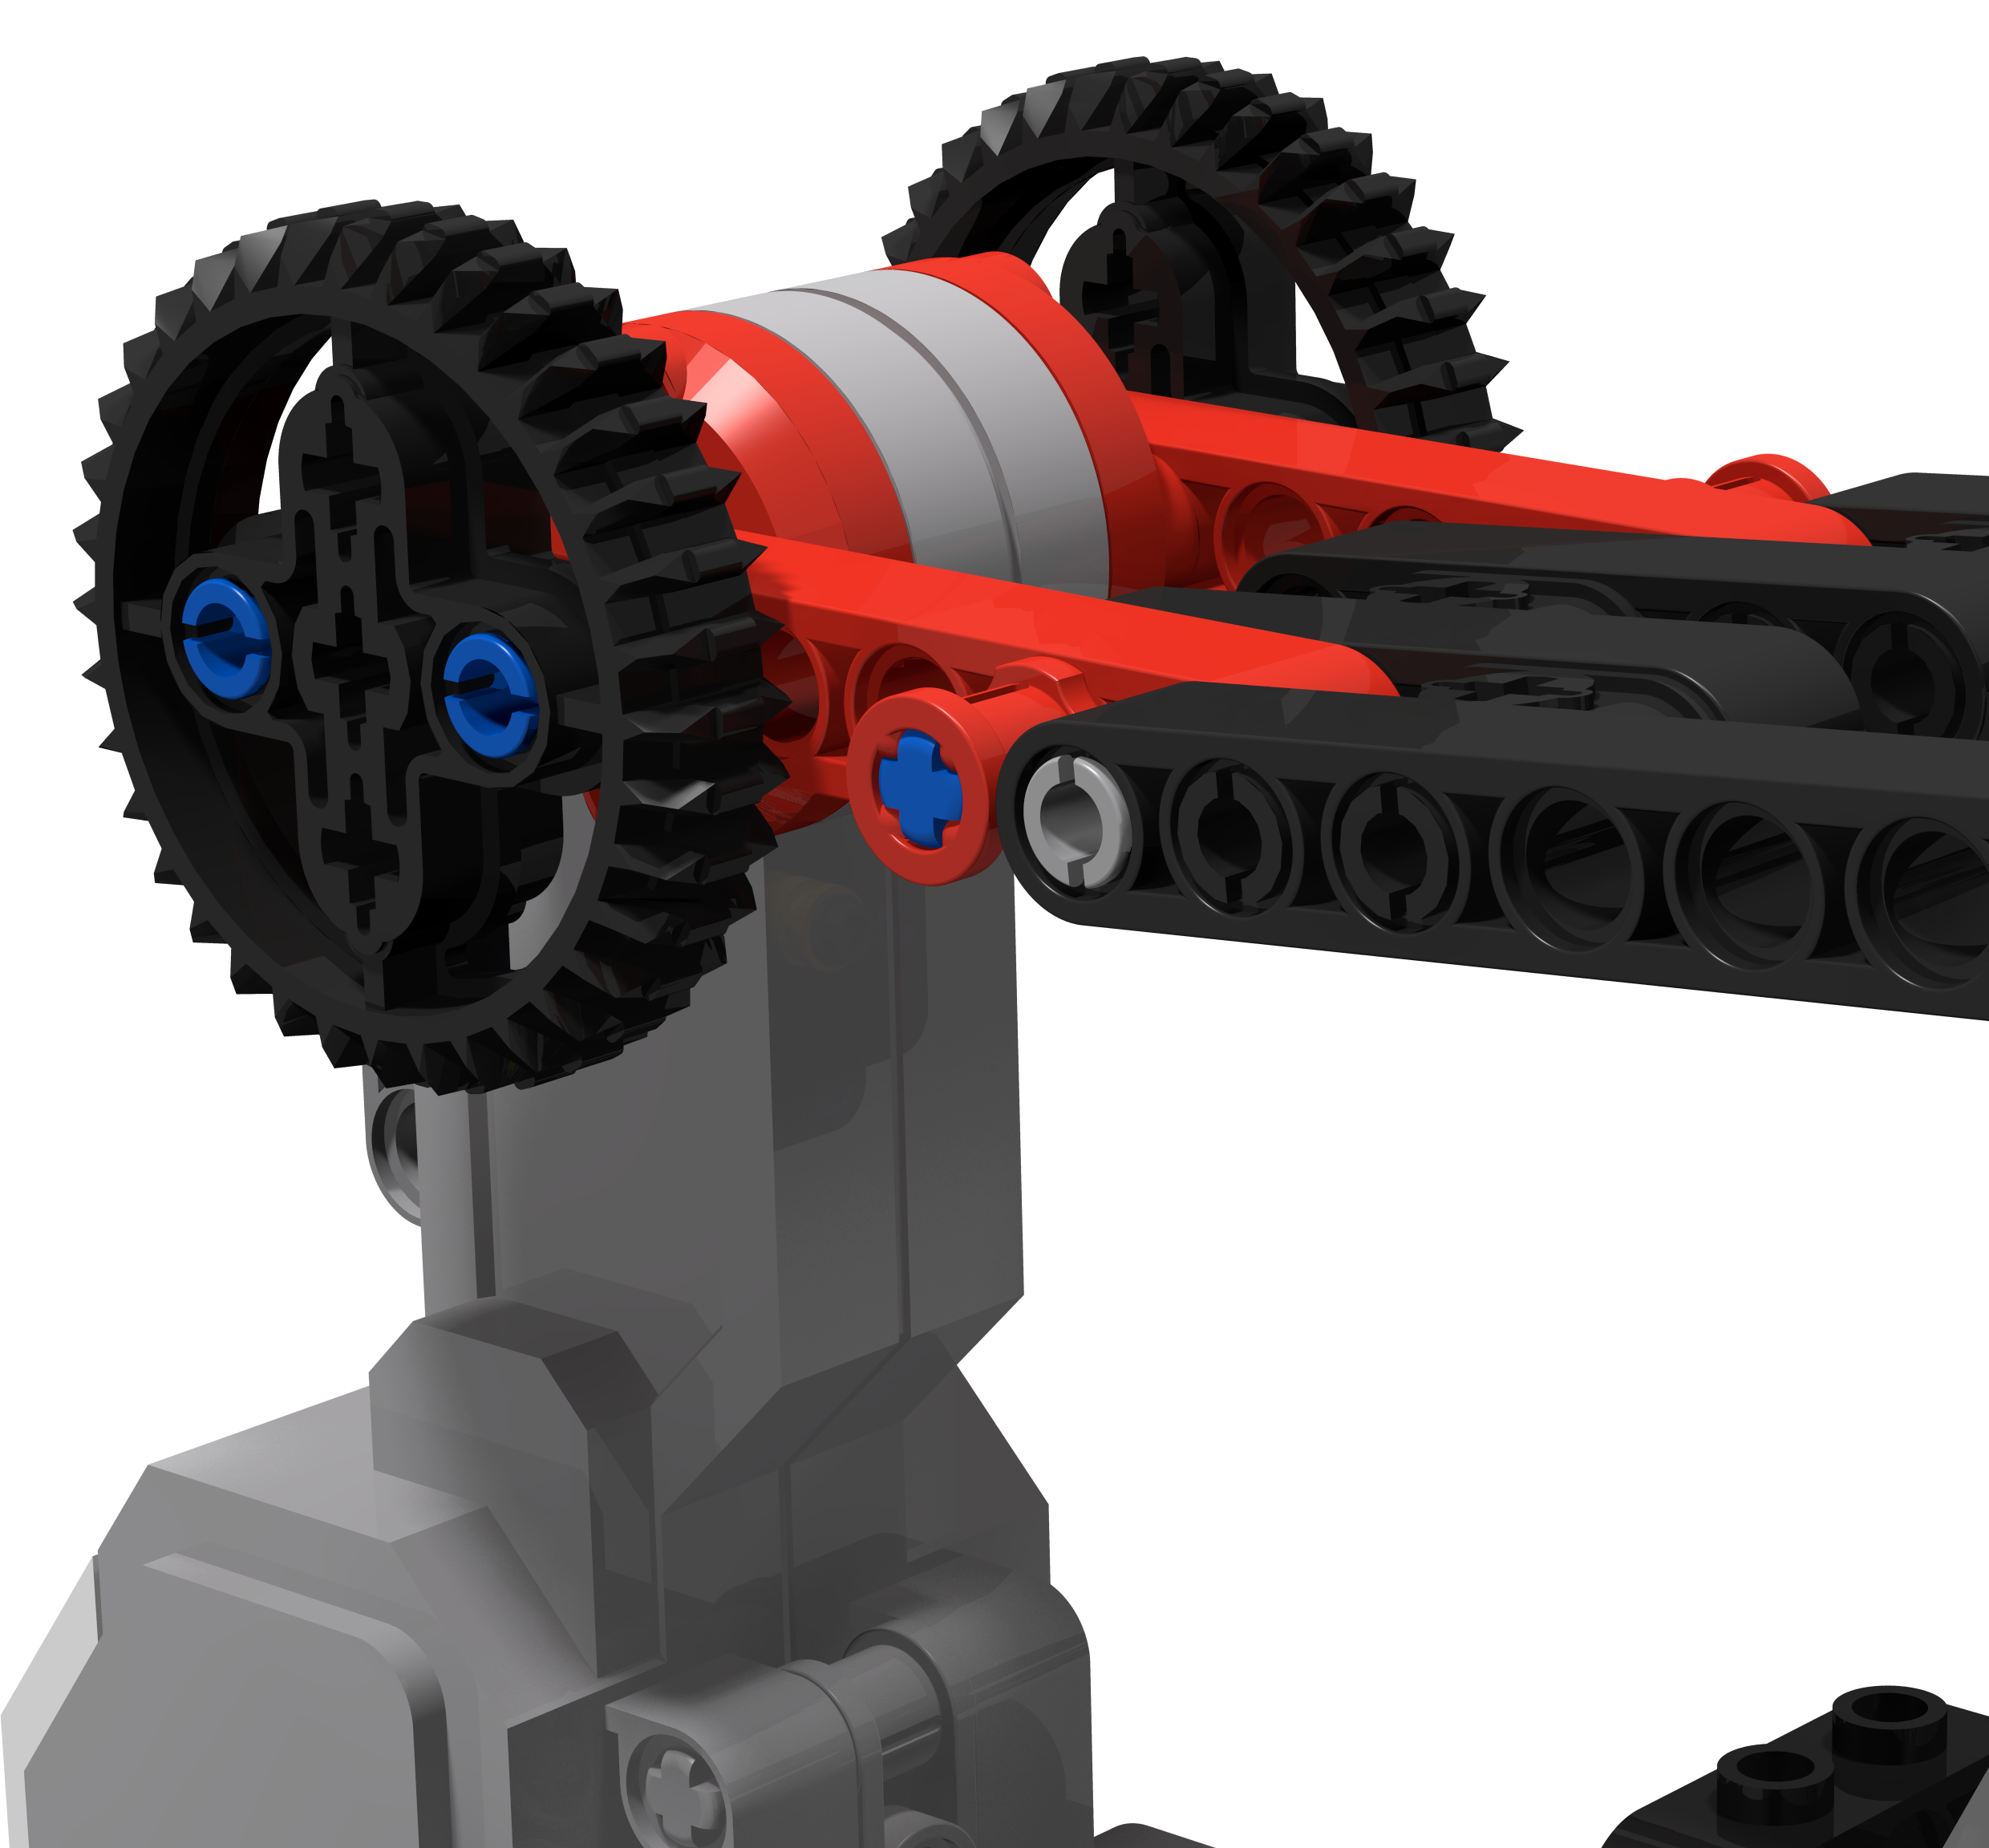
\includegraphics[width=\textwidth]{Resources/Images/rdrInitialiser3.png}
			\caption{\move{x} Arm initialiser}
			\label{fig:rdrInitialiser3}
		\end{subfigure}
		\caption{The initialising gears used for each motor}
		\label{fig:rdrInitialiser}
	\end{figure}
	
	\subsubsection{Fragility and Adaptability}
	
	One of the MkI's greatest flaws was the fragility of the frame that held the \move{x} arm in place. It was also very difficult to adjust the MkI because of the design's complexity. With this in mind, the MkII was constructed of two main modules which could be structurally tested independently. These modules were connected with seven red pins \legopiece{32054} that are easily accessible: if any modifications need to be made to the MkII, the pins can be removed and the modules separated for quick and efficient modification.
	
	\begin{figure}[H]
		\centering
		\begin{subfigure}[b]{0.25\textwidth}
			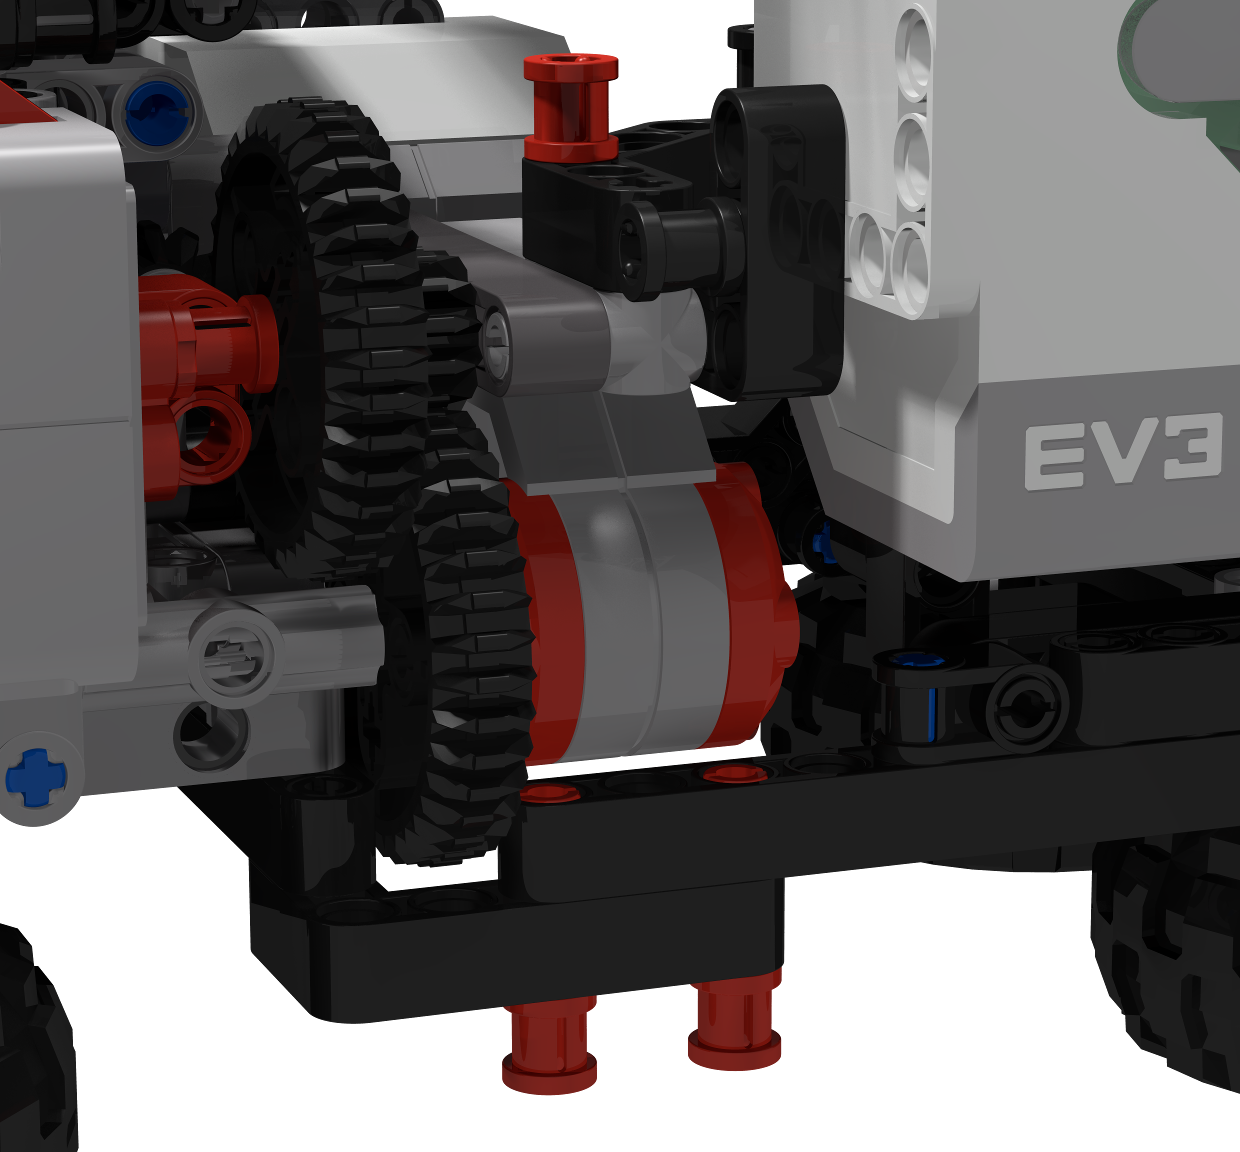
\includegraphics[width=\textwidth]{Resources/Images/rdrModulePins1.png}
			\label{fig:rdrModulePins1}
		\end{subfigure}
		\hspace{10mm}
		\begin{subfigure}[b]{0.25\textwidth}
			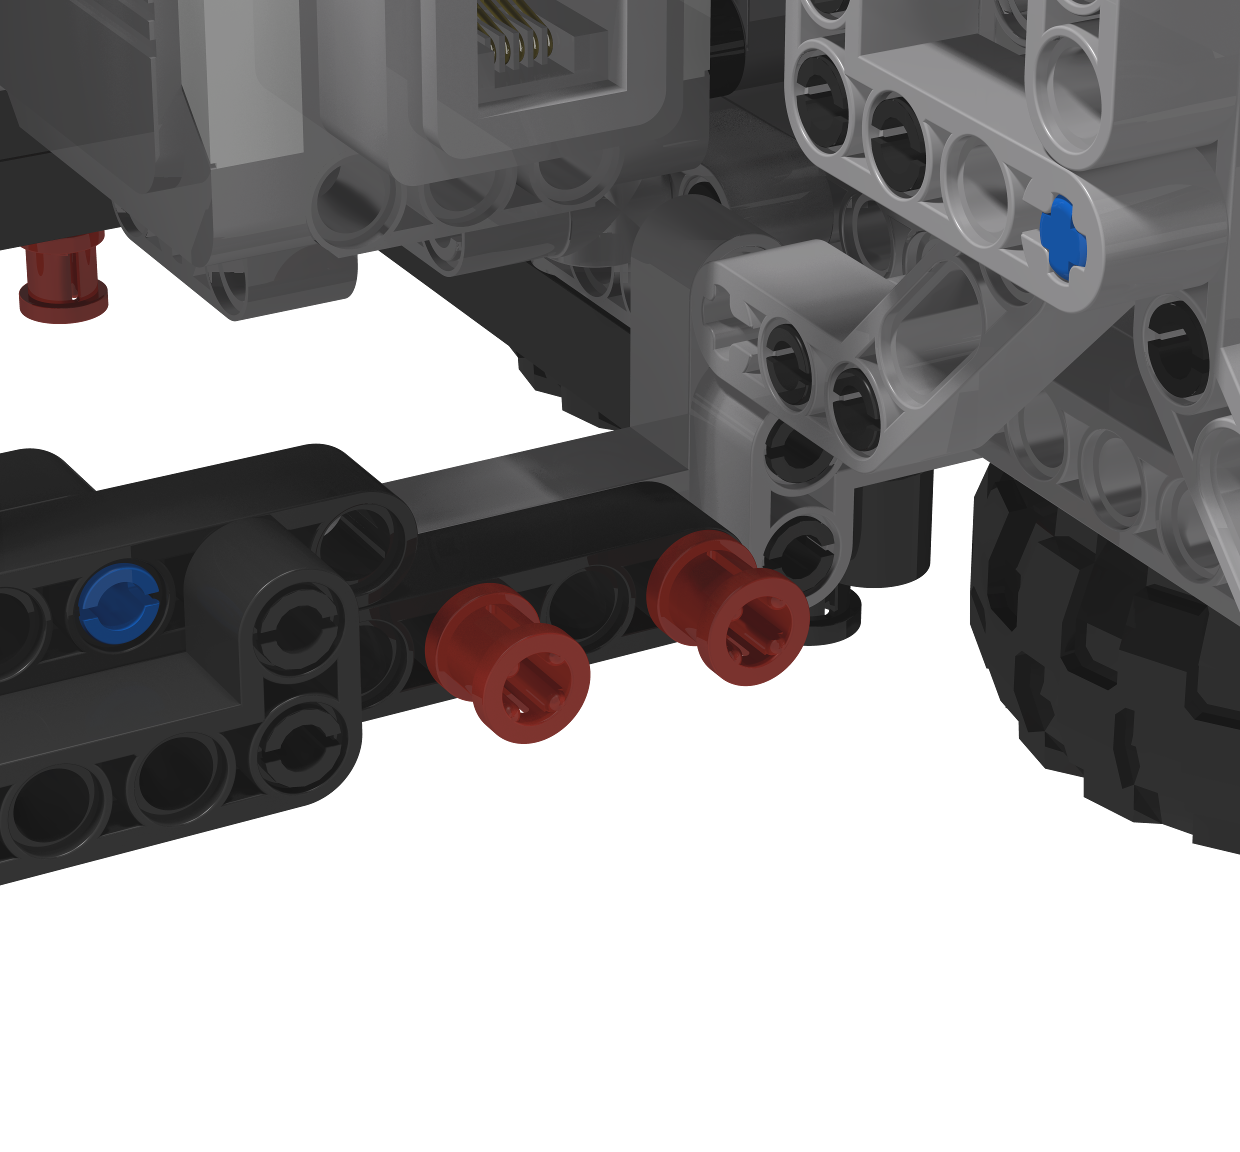
\includegraphics[width=\textwidth]{Resources/Images/rdrModulePins2.png}
			\label{fig:rdrModulePins2}
		\end{subfigure}
		\hspace{10mm}
		\begin{subfigure}[b]{0.25\textwidth}
			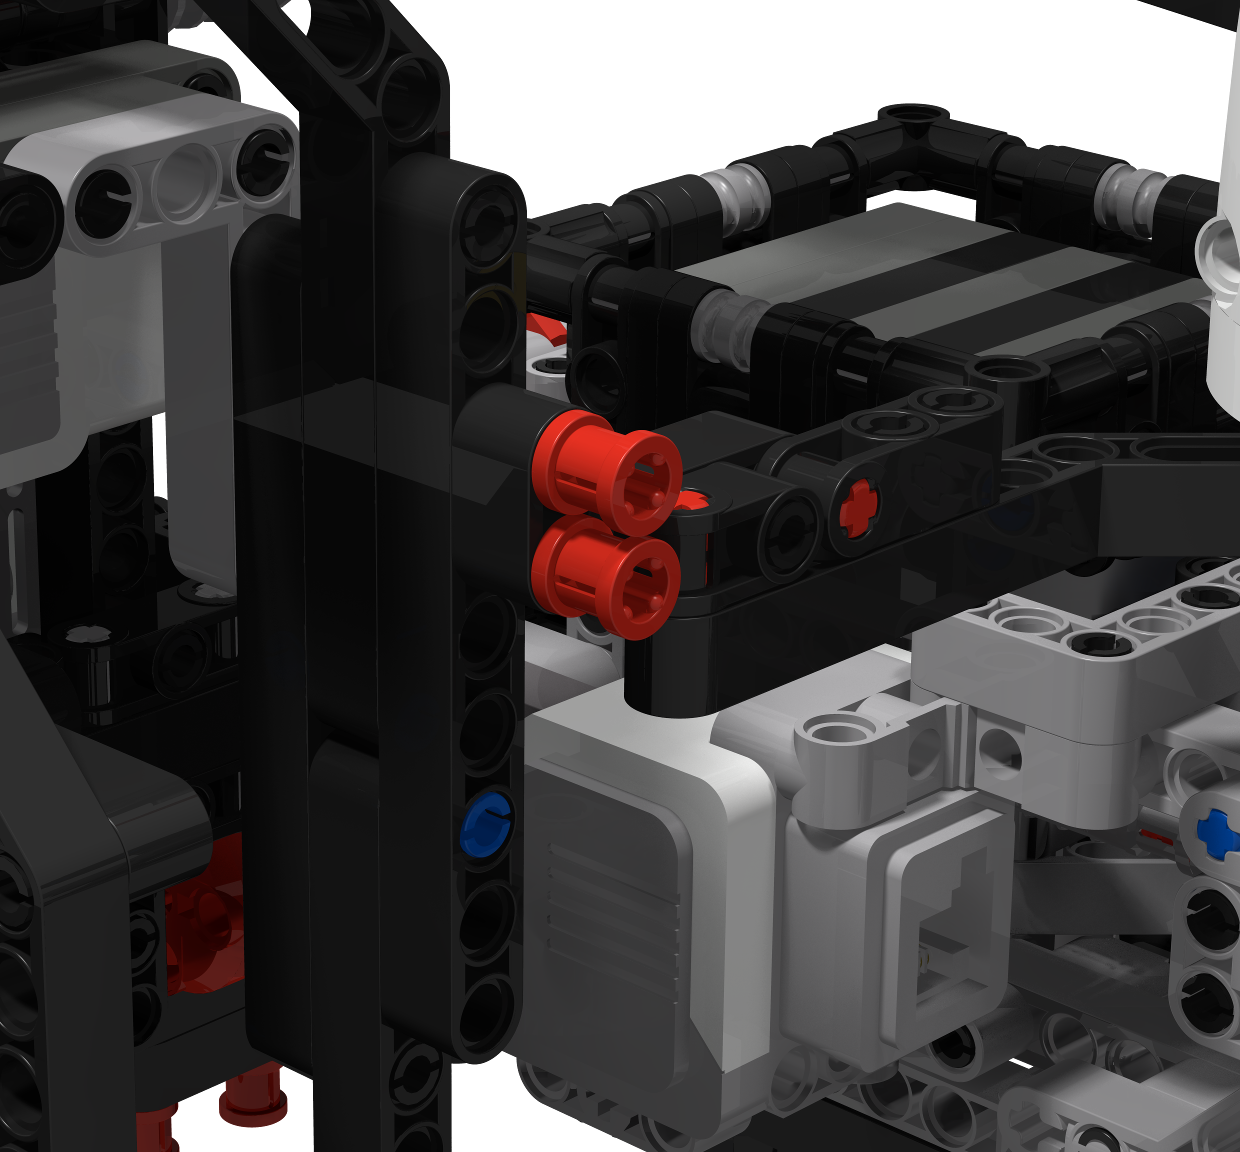
\includegraphics[width=\textwidth]{Resources/Images/rdrModulePins3.png}
			\label{fig:rdrModulePins3}
		\end{subfigure}
		\caption{The pins used for connecting the modules}
		\label{fig:rdrModulePins}
	\end{figure}
	
%	\subsubsection{Battery Usage}
%	
%	The final of the issues discovered by repeated testing of the MkI was how power-hungry the EV3 control brick really is. After only one to one-and-a-half hours of testing, it would run six AA \num{2500} \si{\milli\ampere\hour} batteries completely flat. \lego do sell a rechargeable battery for the EV3, however it's only \num{2050} \si{\milli\ampere\hour} by itself and it costs \pounds81.99 \cite{Lego2018}. A cheaper (and higher capacity) option was to purchase twelve rechargeable \num{2500} \si{\milli\ampere\hour} batteries and a charger for approximately \pounds25. Whilst the EV3 was voraciously consuming the power from six of the batteries, the other six could either be charging or waiting ready. This led to the design and creation of a battery holder attached to the MkII. It holds six AA batteries and has two pins which can be removed to release the batteries, as shown in Figure \ref{fig:imgBatteryHolderOpen}.
%	
%	\begin{figure}[H]
%		\centering
%		\begin{subfigure}[b]{0.27665\textwidth}
%			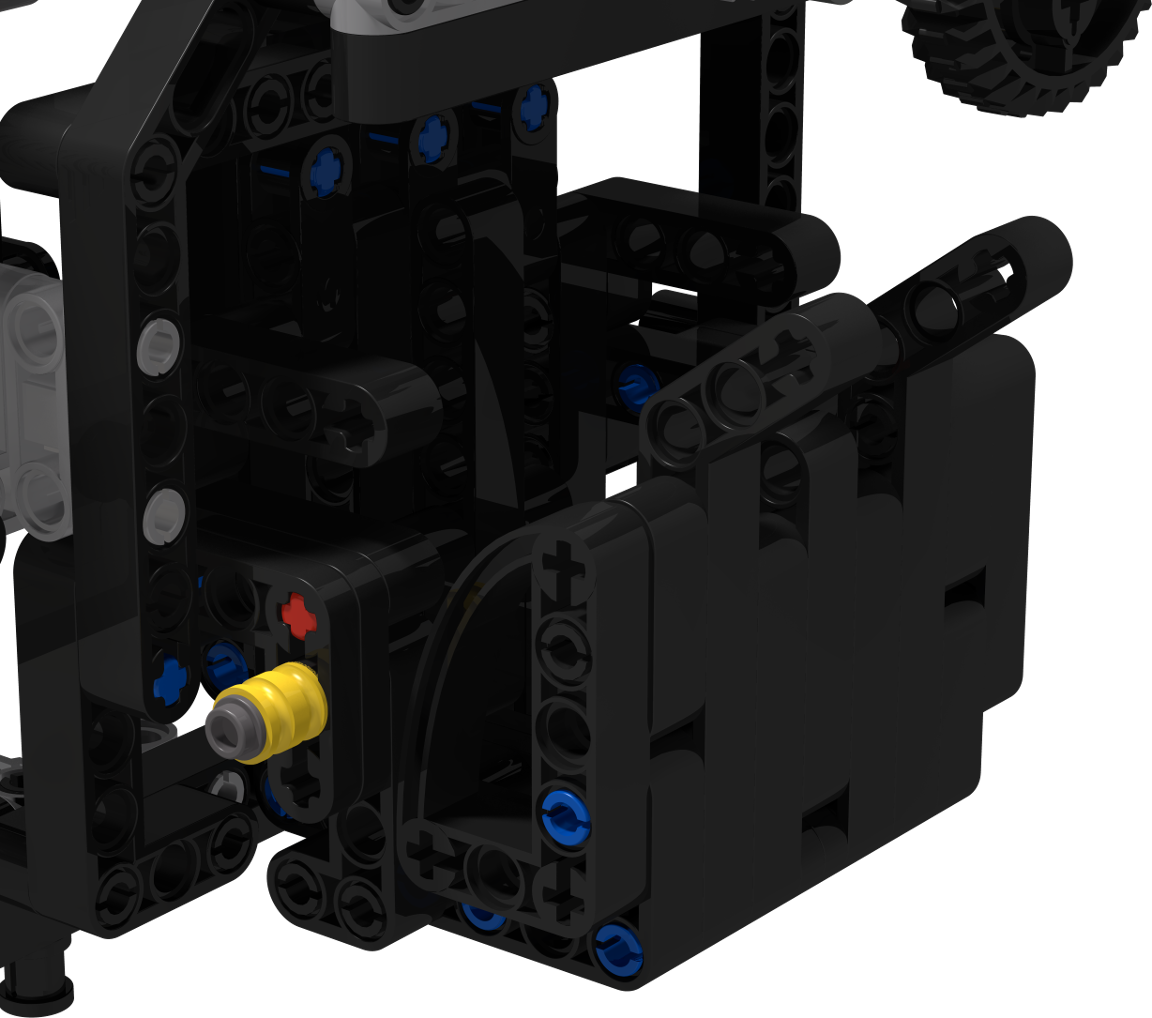
\includegraphics[width=\textwidth]{Resources/Images/rdrBatteryHolder.png}
%			\caption{The design of the battery holder, rendered}
%			\label{fig:rdrBatteryHolder}
%		\end{subfigure}
%		\hspace{10mm}
%		\begin{subfigure}[b]{0.21082\textwidth}
%			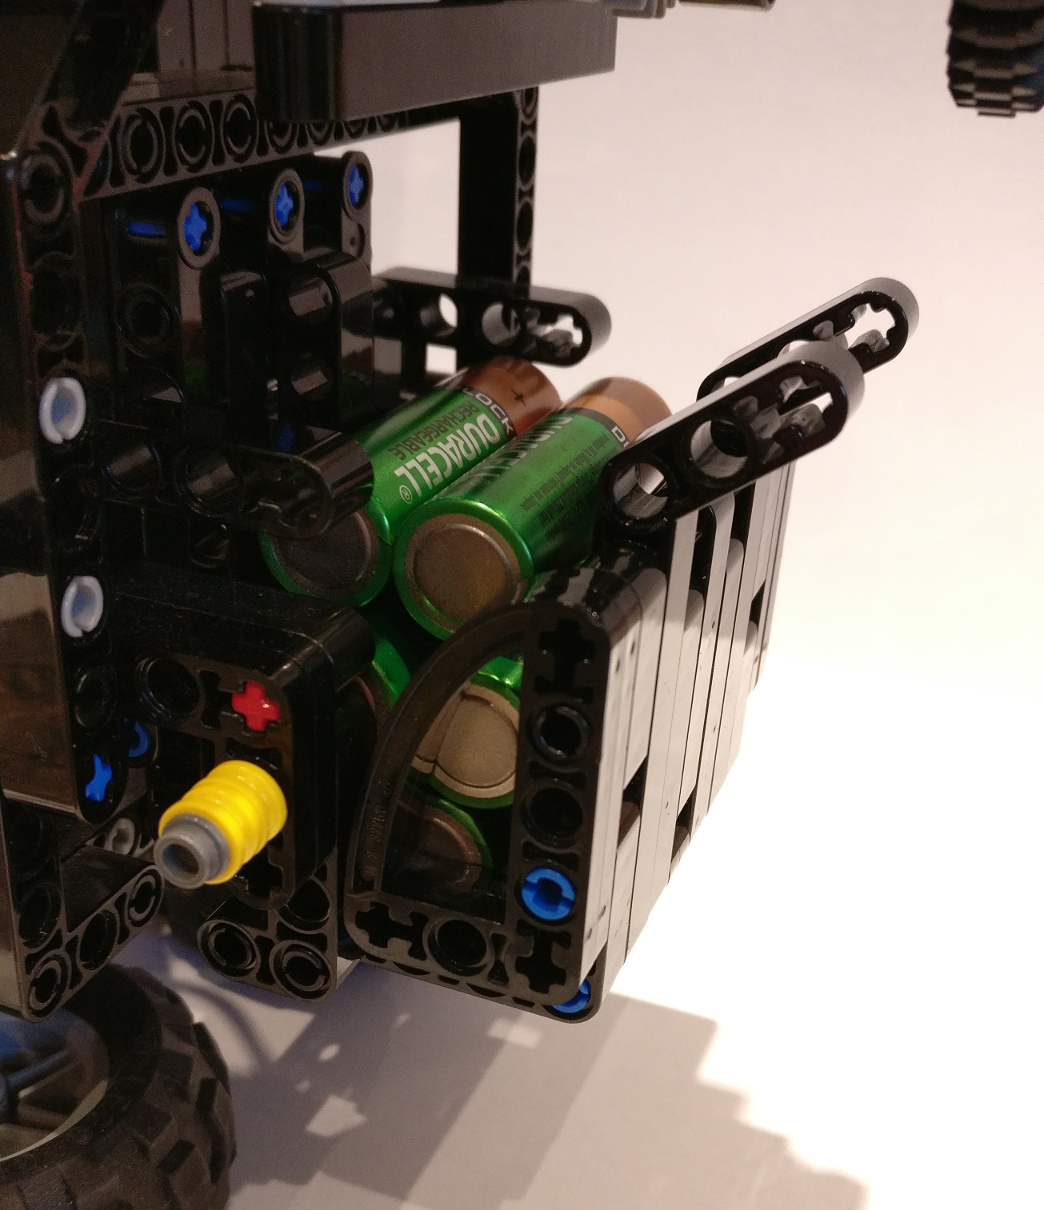
\includegraphics[width=\textwidth]{Resources/Images/imgBatteryHolder.jpg}
%			\caption{Six AA batteries ready for use}
%			\label{fig:imgBatteryHolder}
%		\end{subfigure}
%		\hspace{10mm}
%		\begin{subfigure}[b]{0.26253\textwidth}
%			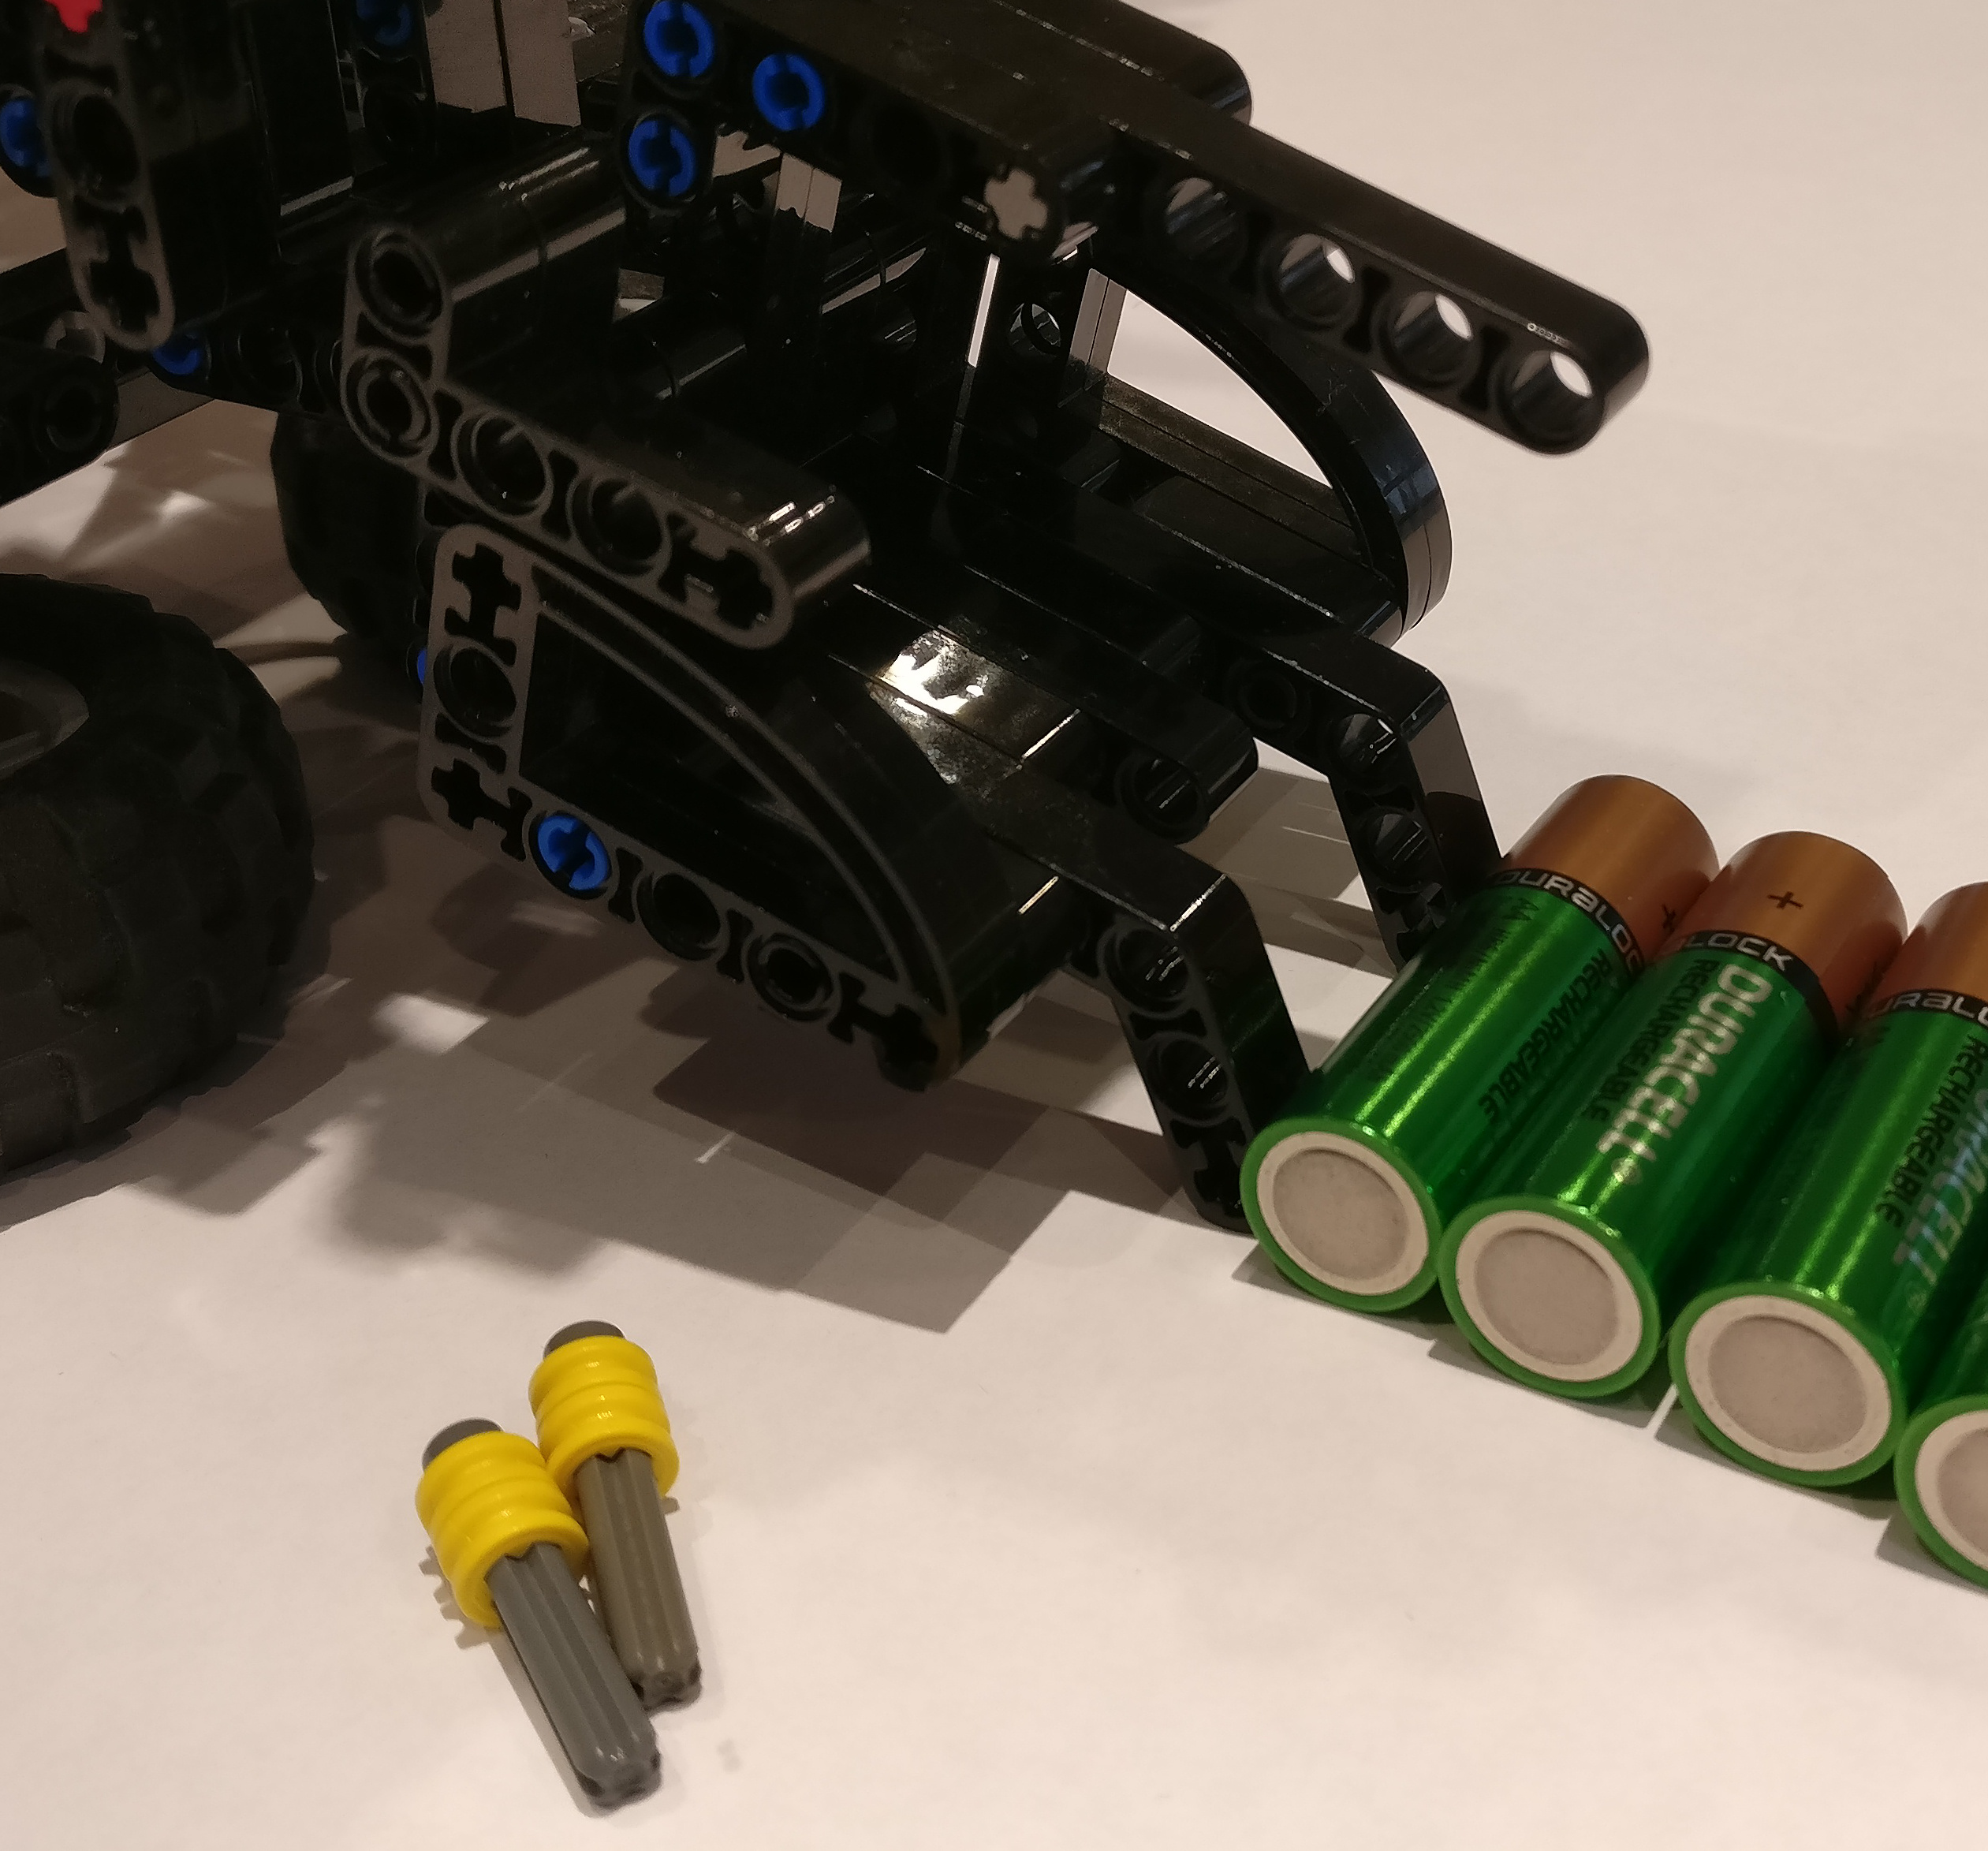
\includegraphics[width=\textwidth]{Resources/Images/imgBatteryHolderOpen.jpg}
%			\caption{The battery holder is opened by removing the pins}
%			\label{fig:imgBatteryHolderOpen}
%		\end{subfigure}
%		\caption{The battery holder, as a rendered model and in real life}
%		\label{fig:batteryHolder}
%	\end{figure}
	
	\subsection{Cradle}

	The MkI cradle had a low accuracy and unreliable rotations, which are both solved by a worm gear \legopiece{4716}. It has been combined with a large gear \legopiece{3649} to create a gear ratio of 1:40, increasing the accuracy of the motor by a factor of forty (see Figure \ref{fig:dwgCradleWormGear}). This also slowed the maximum rotational velocity of the cradle to 0.209 \si{\radian\per\second} (2 RPM) at 7.5\si{\volt}, so a \ang{90} turn will take 7.5 \si{\second}\footnote{This figure is the result of a measurement of the maximum rotational velocity of a large motor, and will fluctuate depending on the voltage supplied by the batteries in the EV3 brick}. A compromise between maximum rotational velocity and accuracy has been found by adding more gears to reduce the ratio. The problem presented by the play in the motor has been successfully minimised due to the unidirectional nature of the gear train.
	
	\begin{figure}[H]
		\centering
		\begin{subfigure}[b]{0.37999\textwidth}
			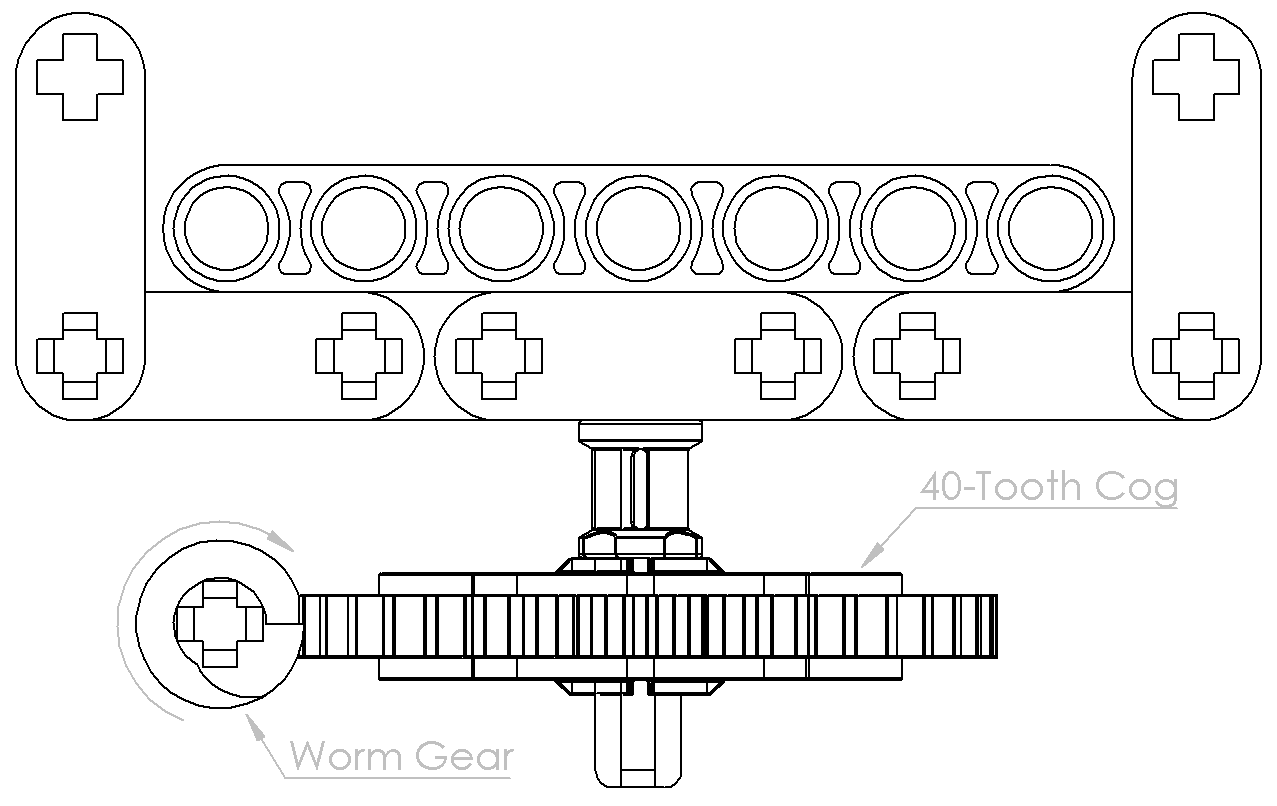
\includegraphics[width=\textwidth]{Resources/Images/dwgCradleWormGear.png}
			\caption{The rotation of the worm gear drives the cradle's rotation}
			\label{fig:dwgCradleWormGear}
		\end{subfigure}
		\hspace{10mm}
		\begin{subfigure}[b]{0.42014\textwidth}
			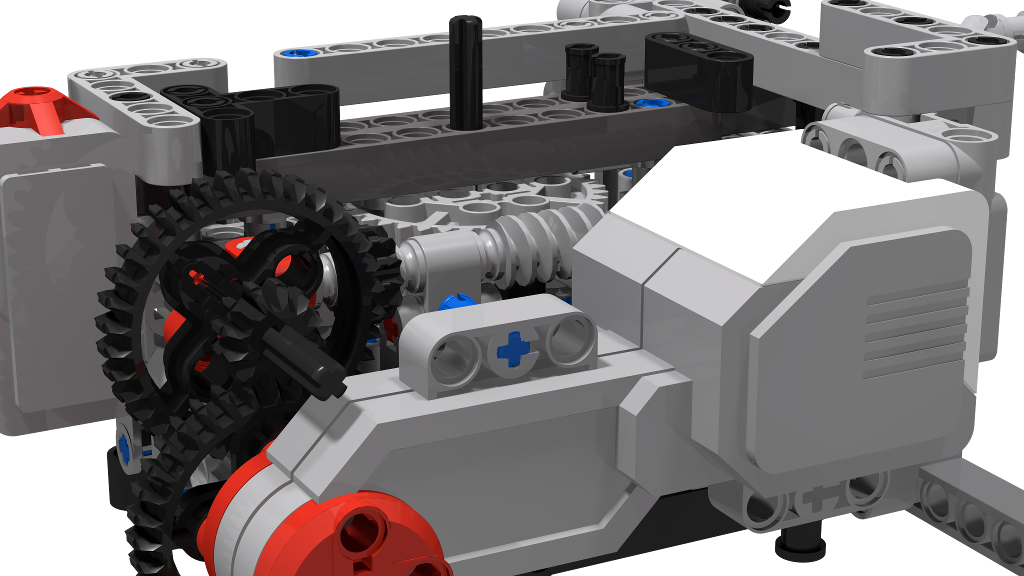
\includegraphics[width=\textwidth]{Resources/Images/rdrCradleWormGear.png}
			\caption{The gear train which provides power to the cradle}
			\label{fig:rdrCradleWormGear}
		\end{subfigure}
		\caption{The battery holder, as a rendered model and in real life}
		\label{fig:cradleWormGear}
	\end{figure}
	
	Figure \ref{fig:rdrCradleWormGear} shows how the cradle is driven by a large motor. A large 36-tooth gear \legopiece{32498} is directly attached to the rotor. This gear drives a 12-tooth gear \legopiece{32270} to triple the rotational velocity at that point of the gear train. This connection is immediately repeated and used to create a \ang{90} turn onto the shaft with the worm gear. The total speed ration of the gear train is 1:4.44, which means that the maximum rotational velocity of the cradle will be 1.84 \si{\radian\per\second} (17.6 RPM) at 7.5\si{\volt} and the original torque is increased from 0.0173 \si{\newton\metre} to 0.0768 \si{\newton\metre}. The vertical black shaft seen at the top of Figure \ref{fig:rdrCradleWormGear} provides a mounting point for the cradle.
	
	\subsection{X-Move Arm}
    
    The largest change between the two design iterations was the complete update of the \move{x} arm - in functionality, aesthetics, and reliability. Where the MkI \move{x} arm relied on pushing the Cube, the MkII pulls the Cube towards it. This creates a much more controlled movement, as the Cube is bound on all four sides at all times. As shown in Figure \ref{fig:rdrXMoveBlock}, the Cube cannot fall out of the cradle during the \enquote{pull} part of the rotation due to the small right-angled piece \legopiece{32526} behind the cradle. The pulling motion causes the Cube's rotation, then the Cube is immediately pushed back into the cradle to complete the move.
   	
	\begin{figure}[H]
		\centering
		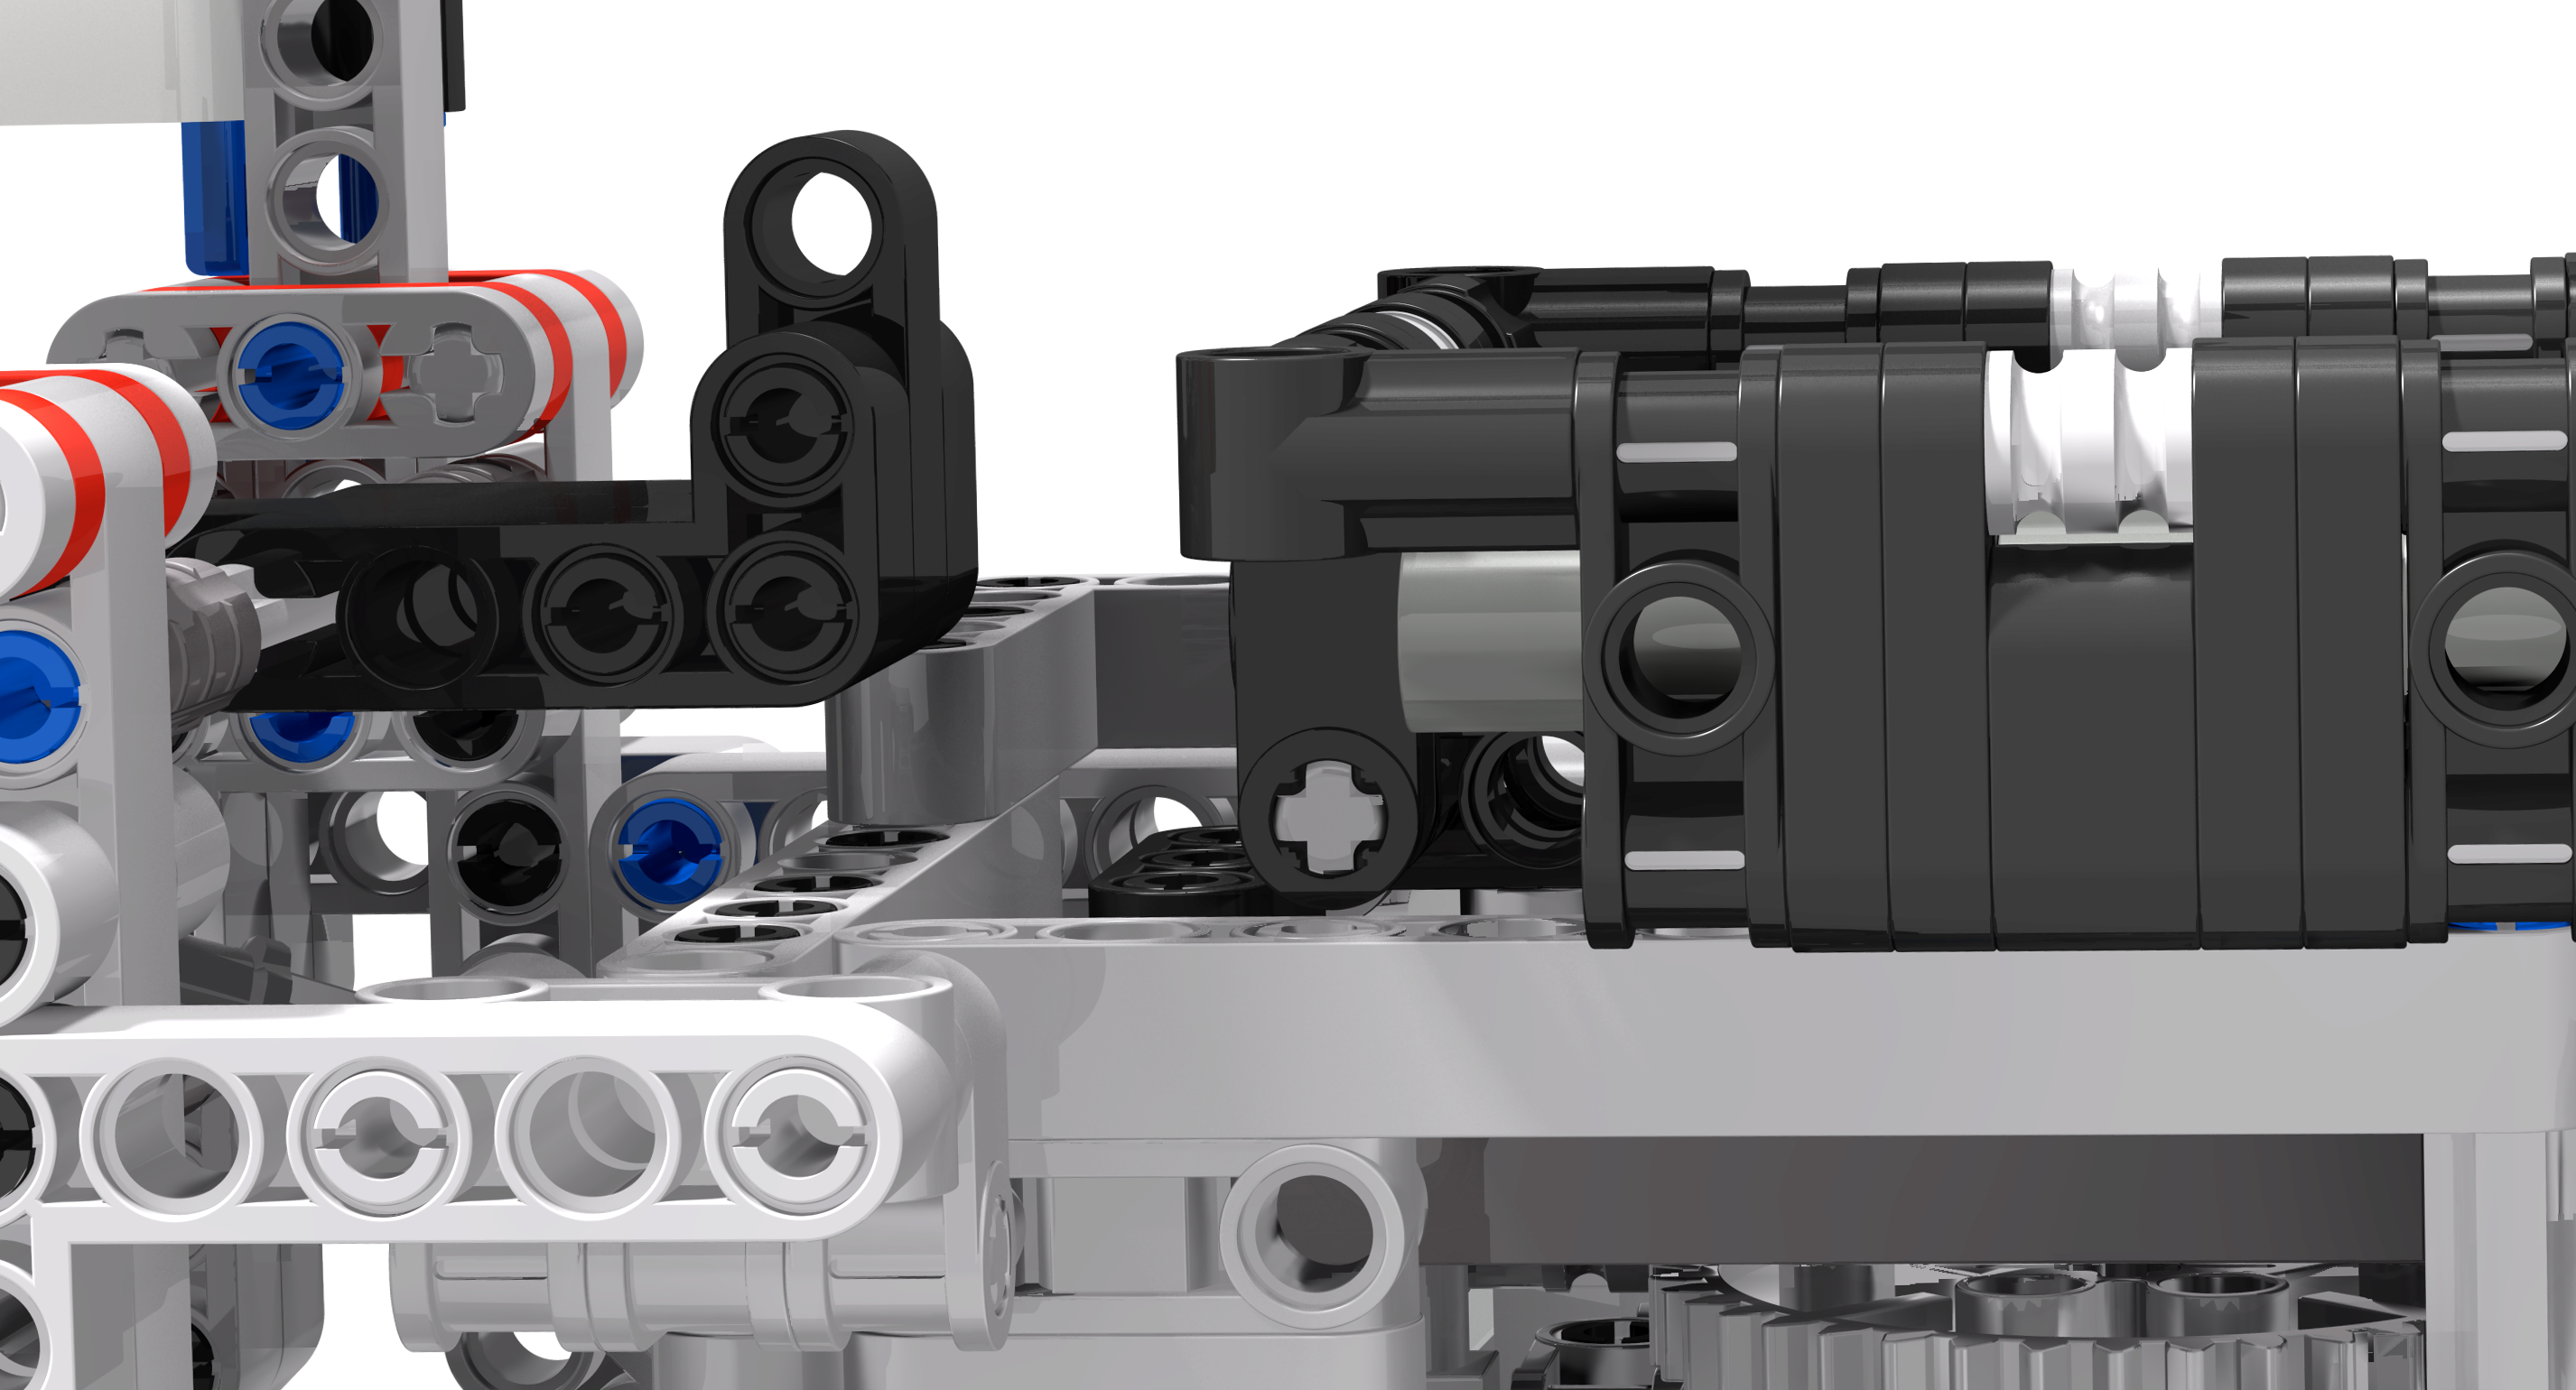
\includegraphics[width=0.4\textwidth]{Resources/Images/rdrXMoveBlock.png}
		\caption{A side elevation to show the pieces which block the Cube from falling}
		\label{fig:rdrXMoveBlock}
   	\end{figure}
   
    The arm is controlled by a single large motor, and is suspended from a tall frame by a liftarm which is free to pivot at both ends. This means that the arm can move \tit{along} the Z axis as well as about the X axis - albeit with limited freedom. Figure \ref{fig:rdrXMoveRenders} shows the \enquote{keyframes} for an \move{x}: 
    
    \begin{enumerate}[a)]
    	\item Starting position, the front of the arm is just touching the \face{f}
    	\item Maximum pull position, the Cube has rotated and is resting on the block piece from Figure \ref{fig:rdrXMoveBlock}
    	\item The Cube is pushed back into the cradle
    	\item Push is completed
    	\item The arm moves out of the way to end the \move{x}
    \end{enumerate}
    
   	\begin{figure}[H]
    	\centering
    	\begin{subfigure}[b]{0.25\textwidth}
    		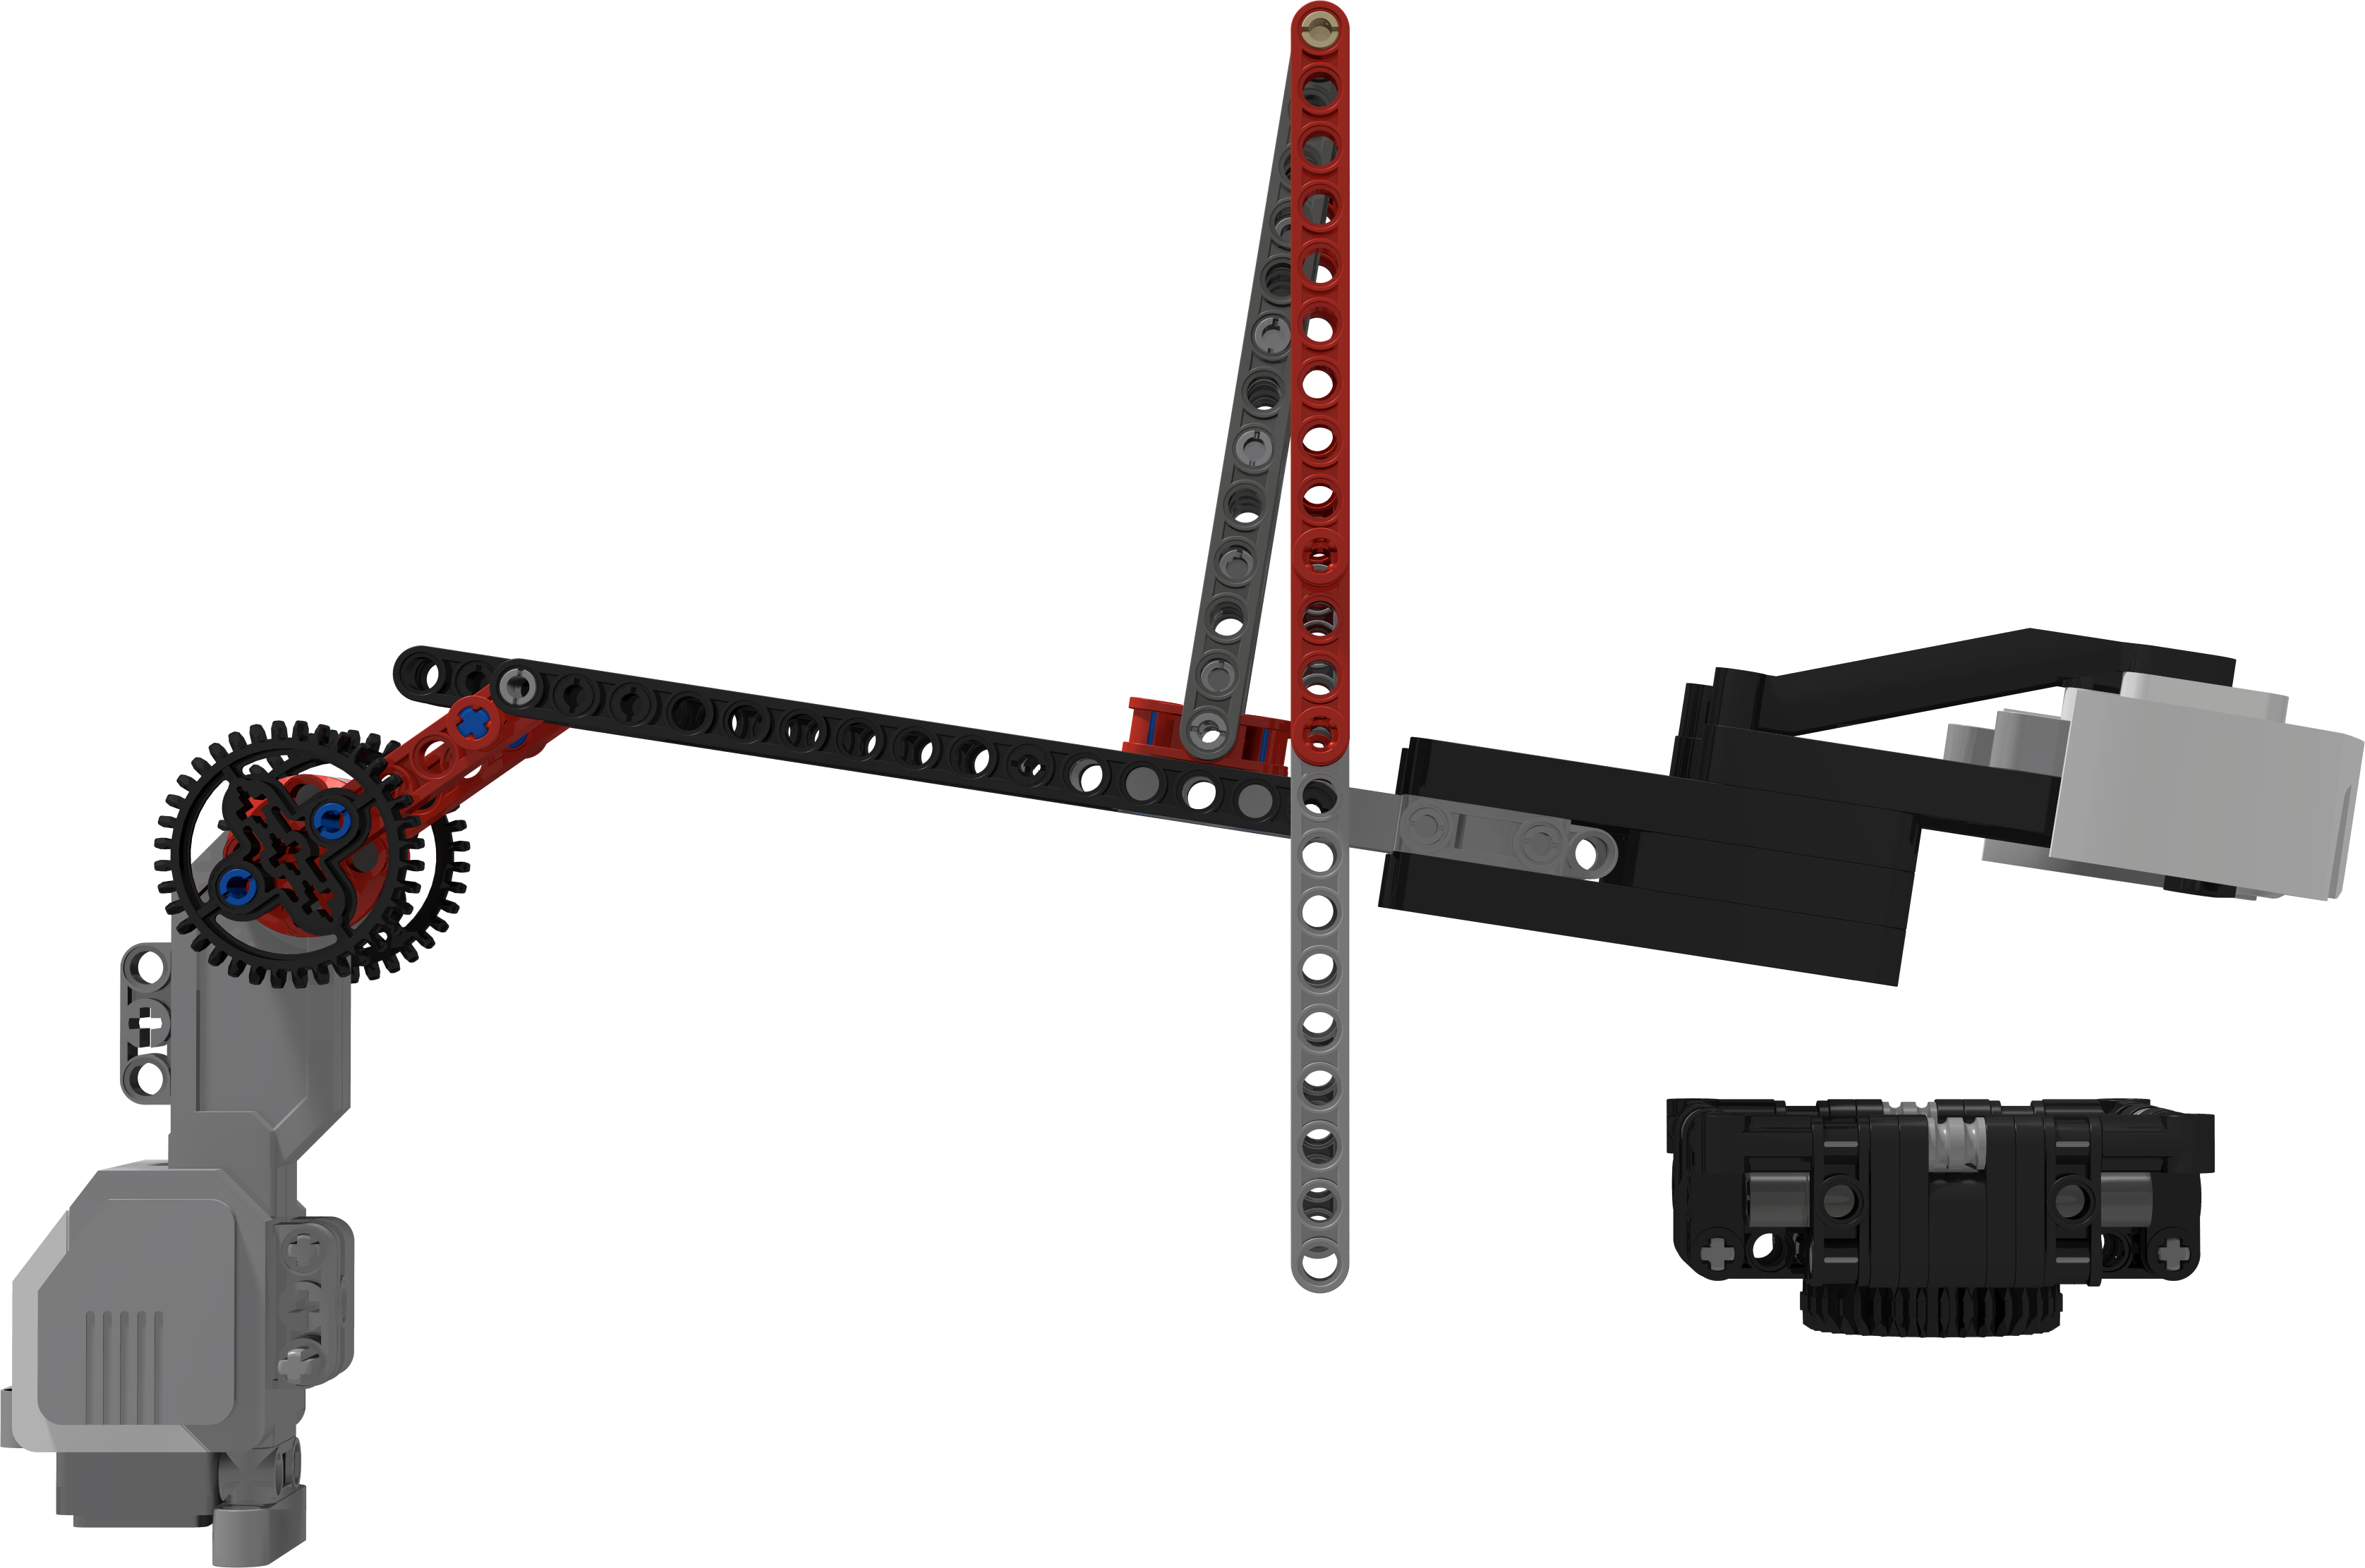
\includegraphics[width=\textwidth]{Resources/Images/rdrXMoveArmLowered.png}
    		\caption{}
    		\label{fig:rdrXMoveArmLowered}
    	\end{subfigure}
    	\hspace{10mm}
    	\begin{subfigure}[b]{0.25\textwidth}
    		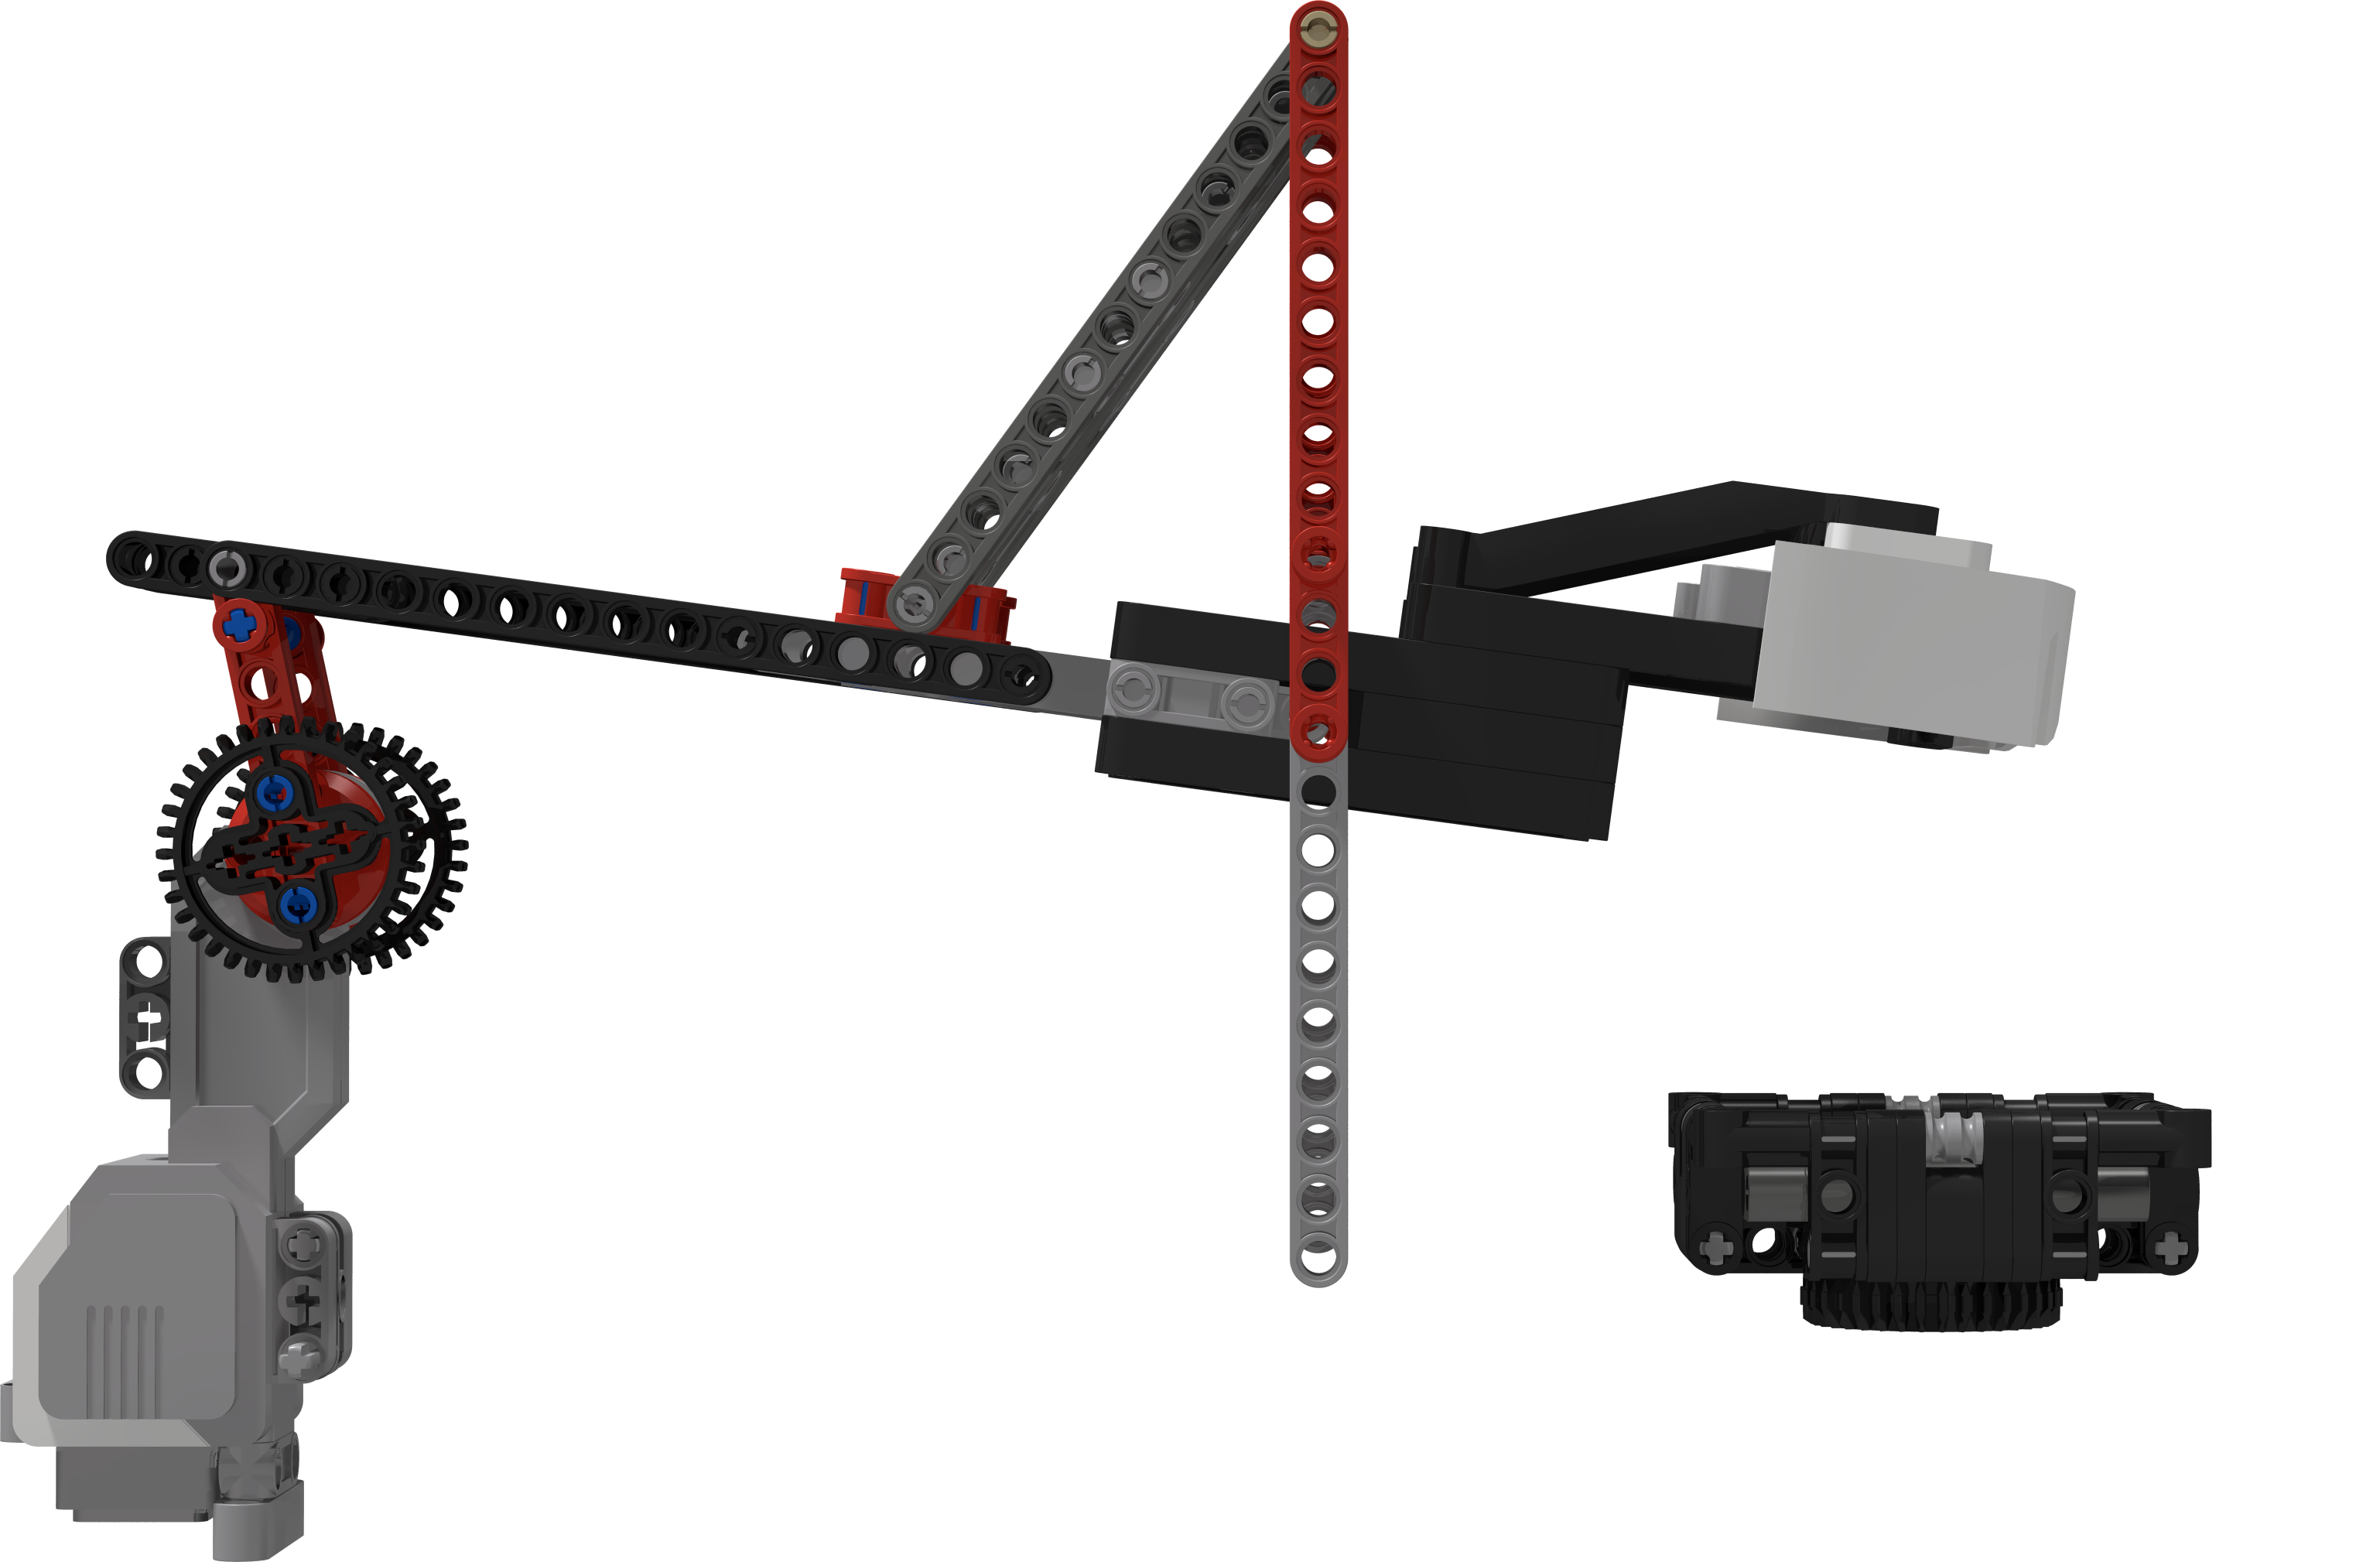
\includegraphics[width=\textwidth]{Resources/Images/rdrXMoveArmPulling.png}
    		\caption{}
    		\label{fig:rdrXMoveArmPulling}
    	\end{subfigure}
    	\hspace{10mm}
    	\begin{subfigure}[b]{0.25\textwidth}
    		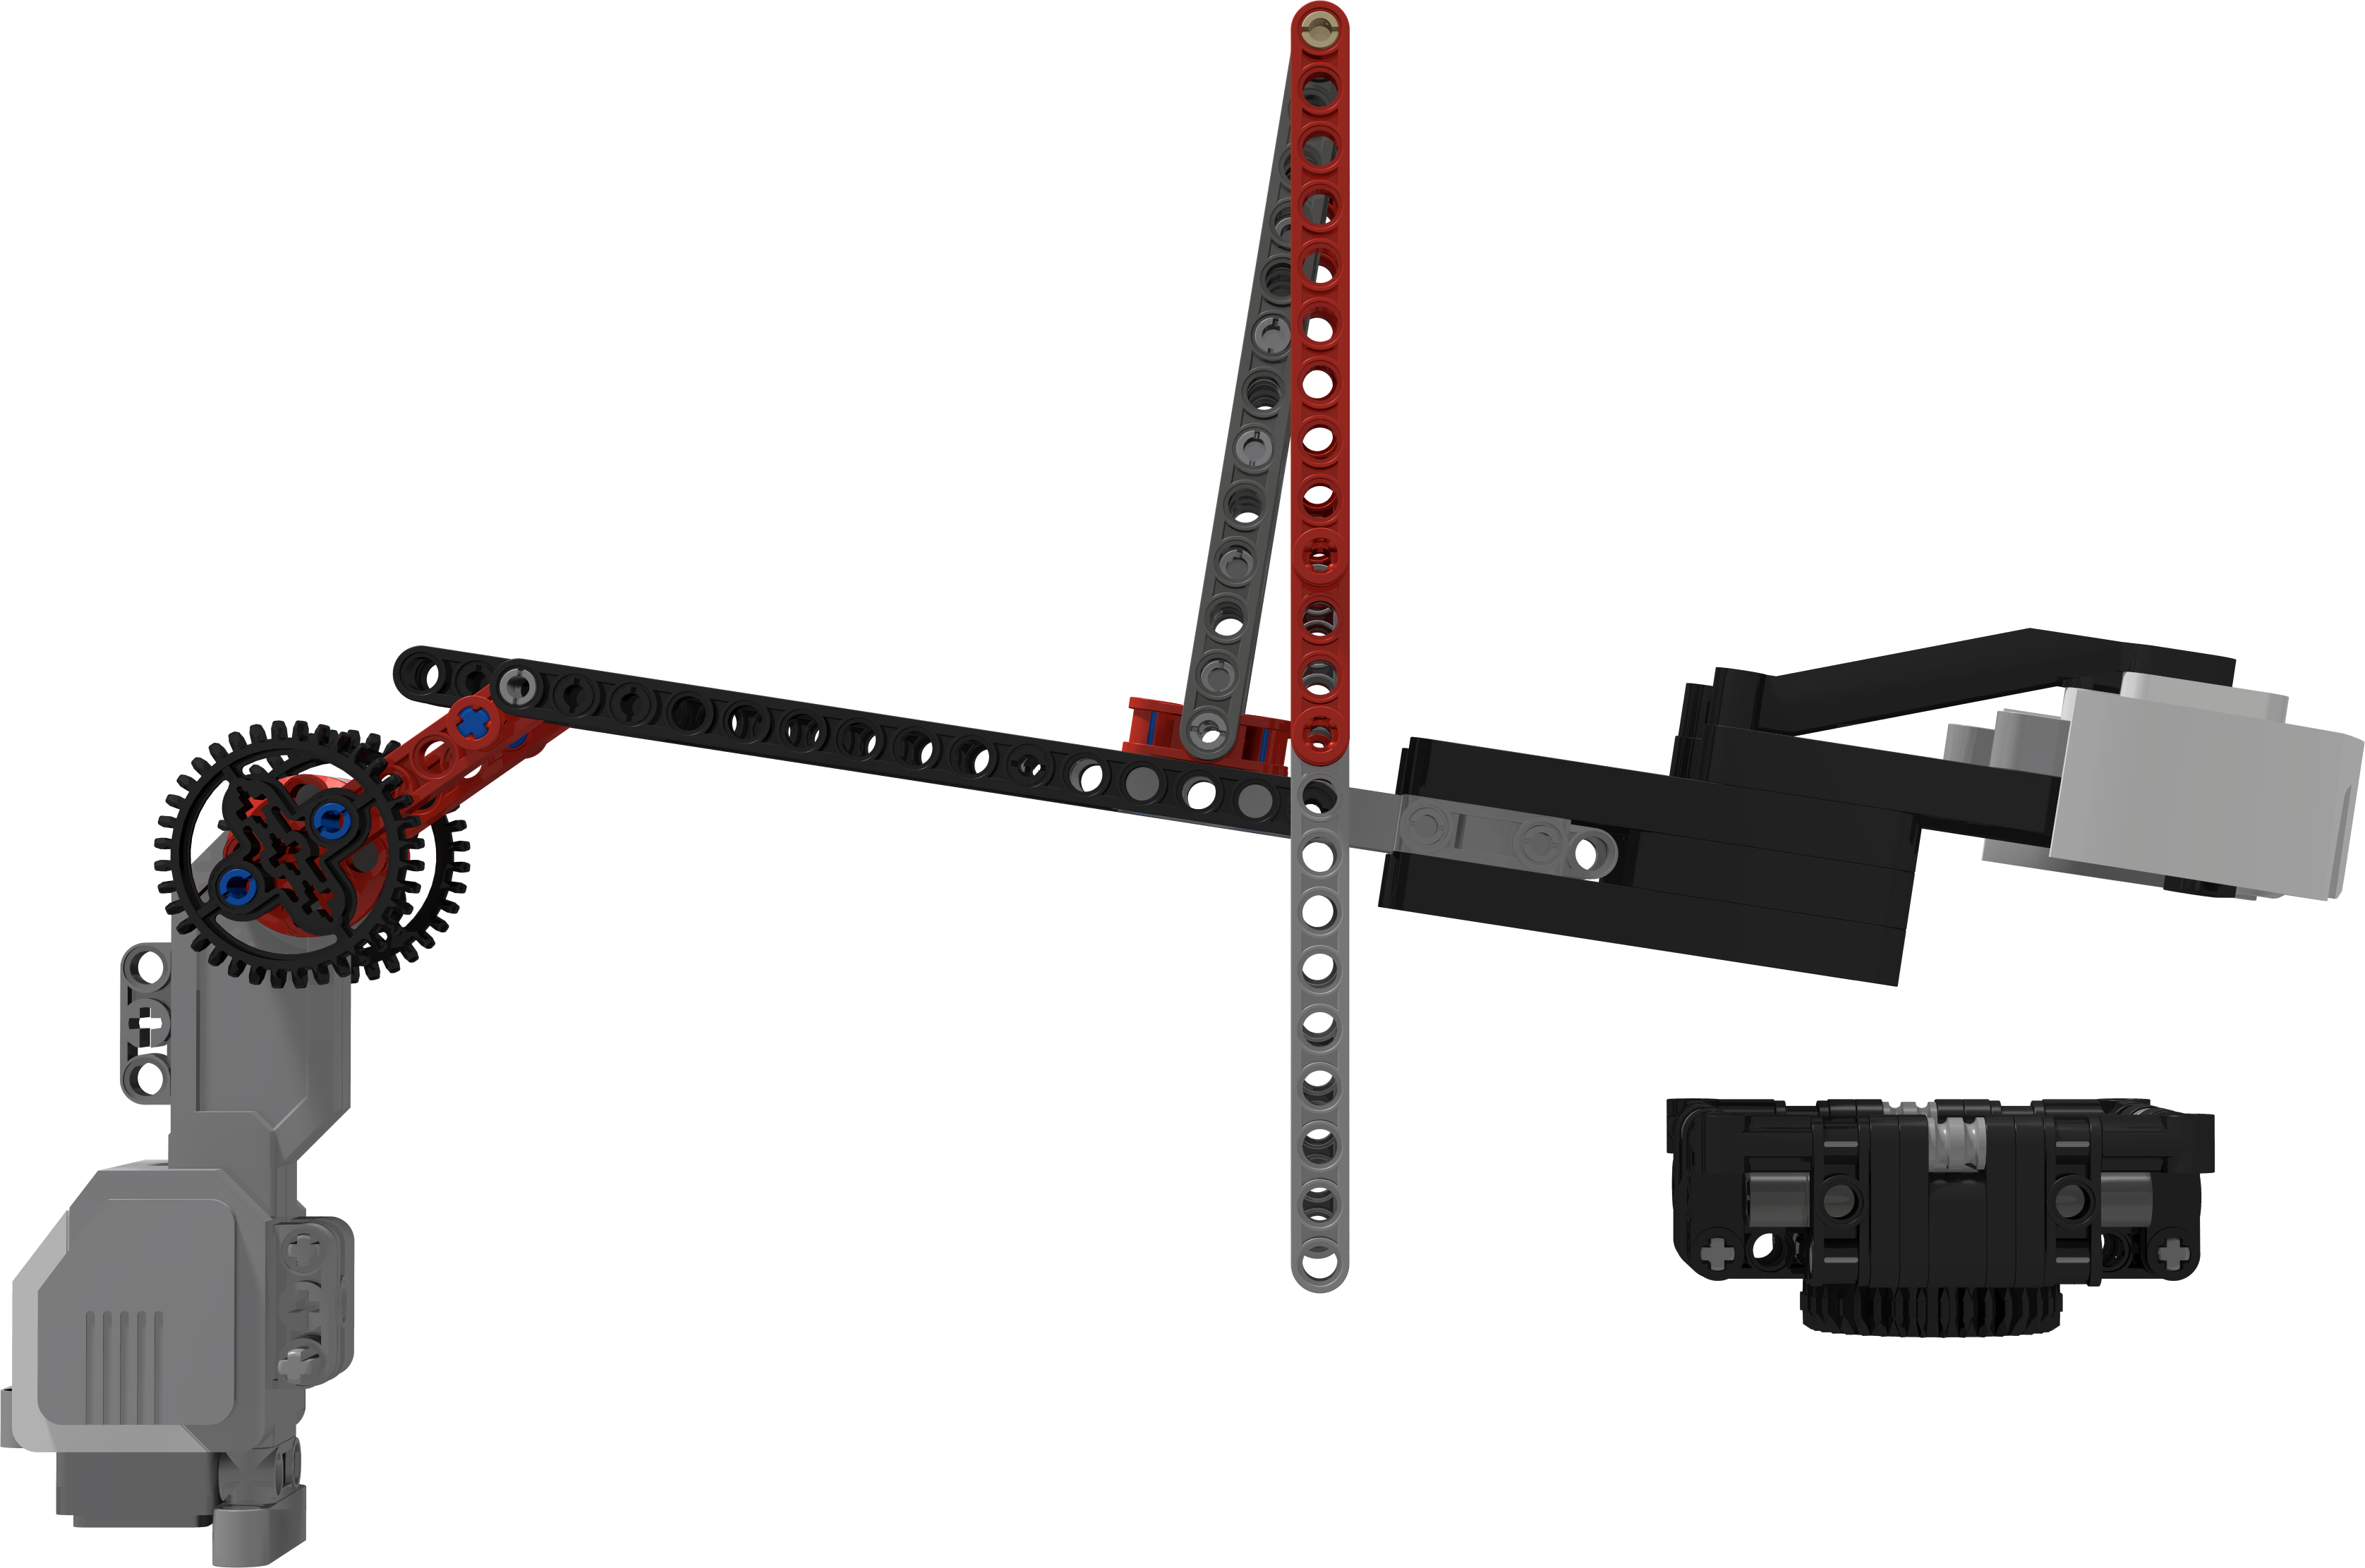
\includegraphics[width=\textwidth]{Resources/Images/rdrXMoveArmLowered.png}
    		\caption{}
    		\label{fig:rdrXMoveArmLowered2}
    	\end{subfigure}
    	\begin{subfigure}[b]{0.25\textwidth}
    		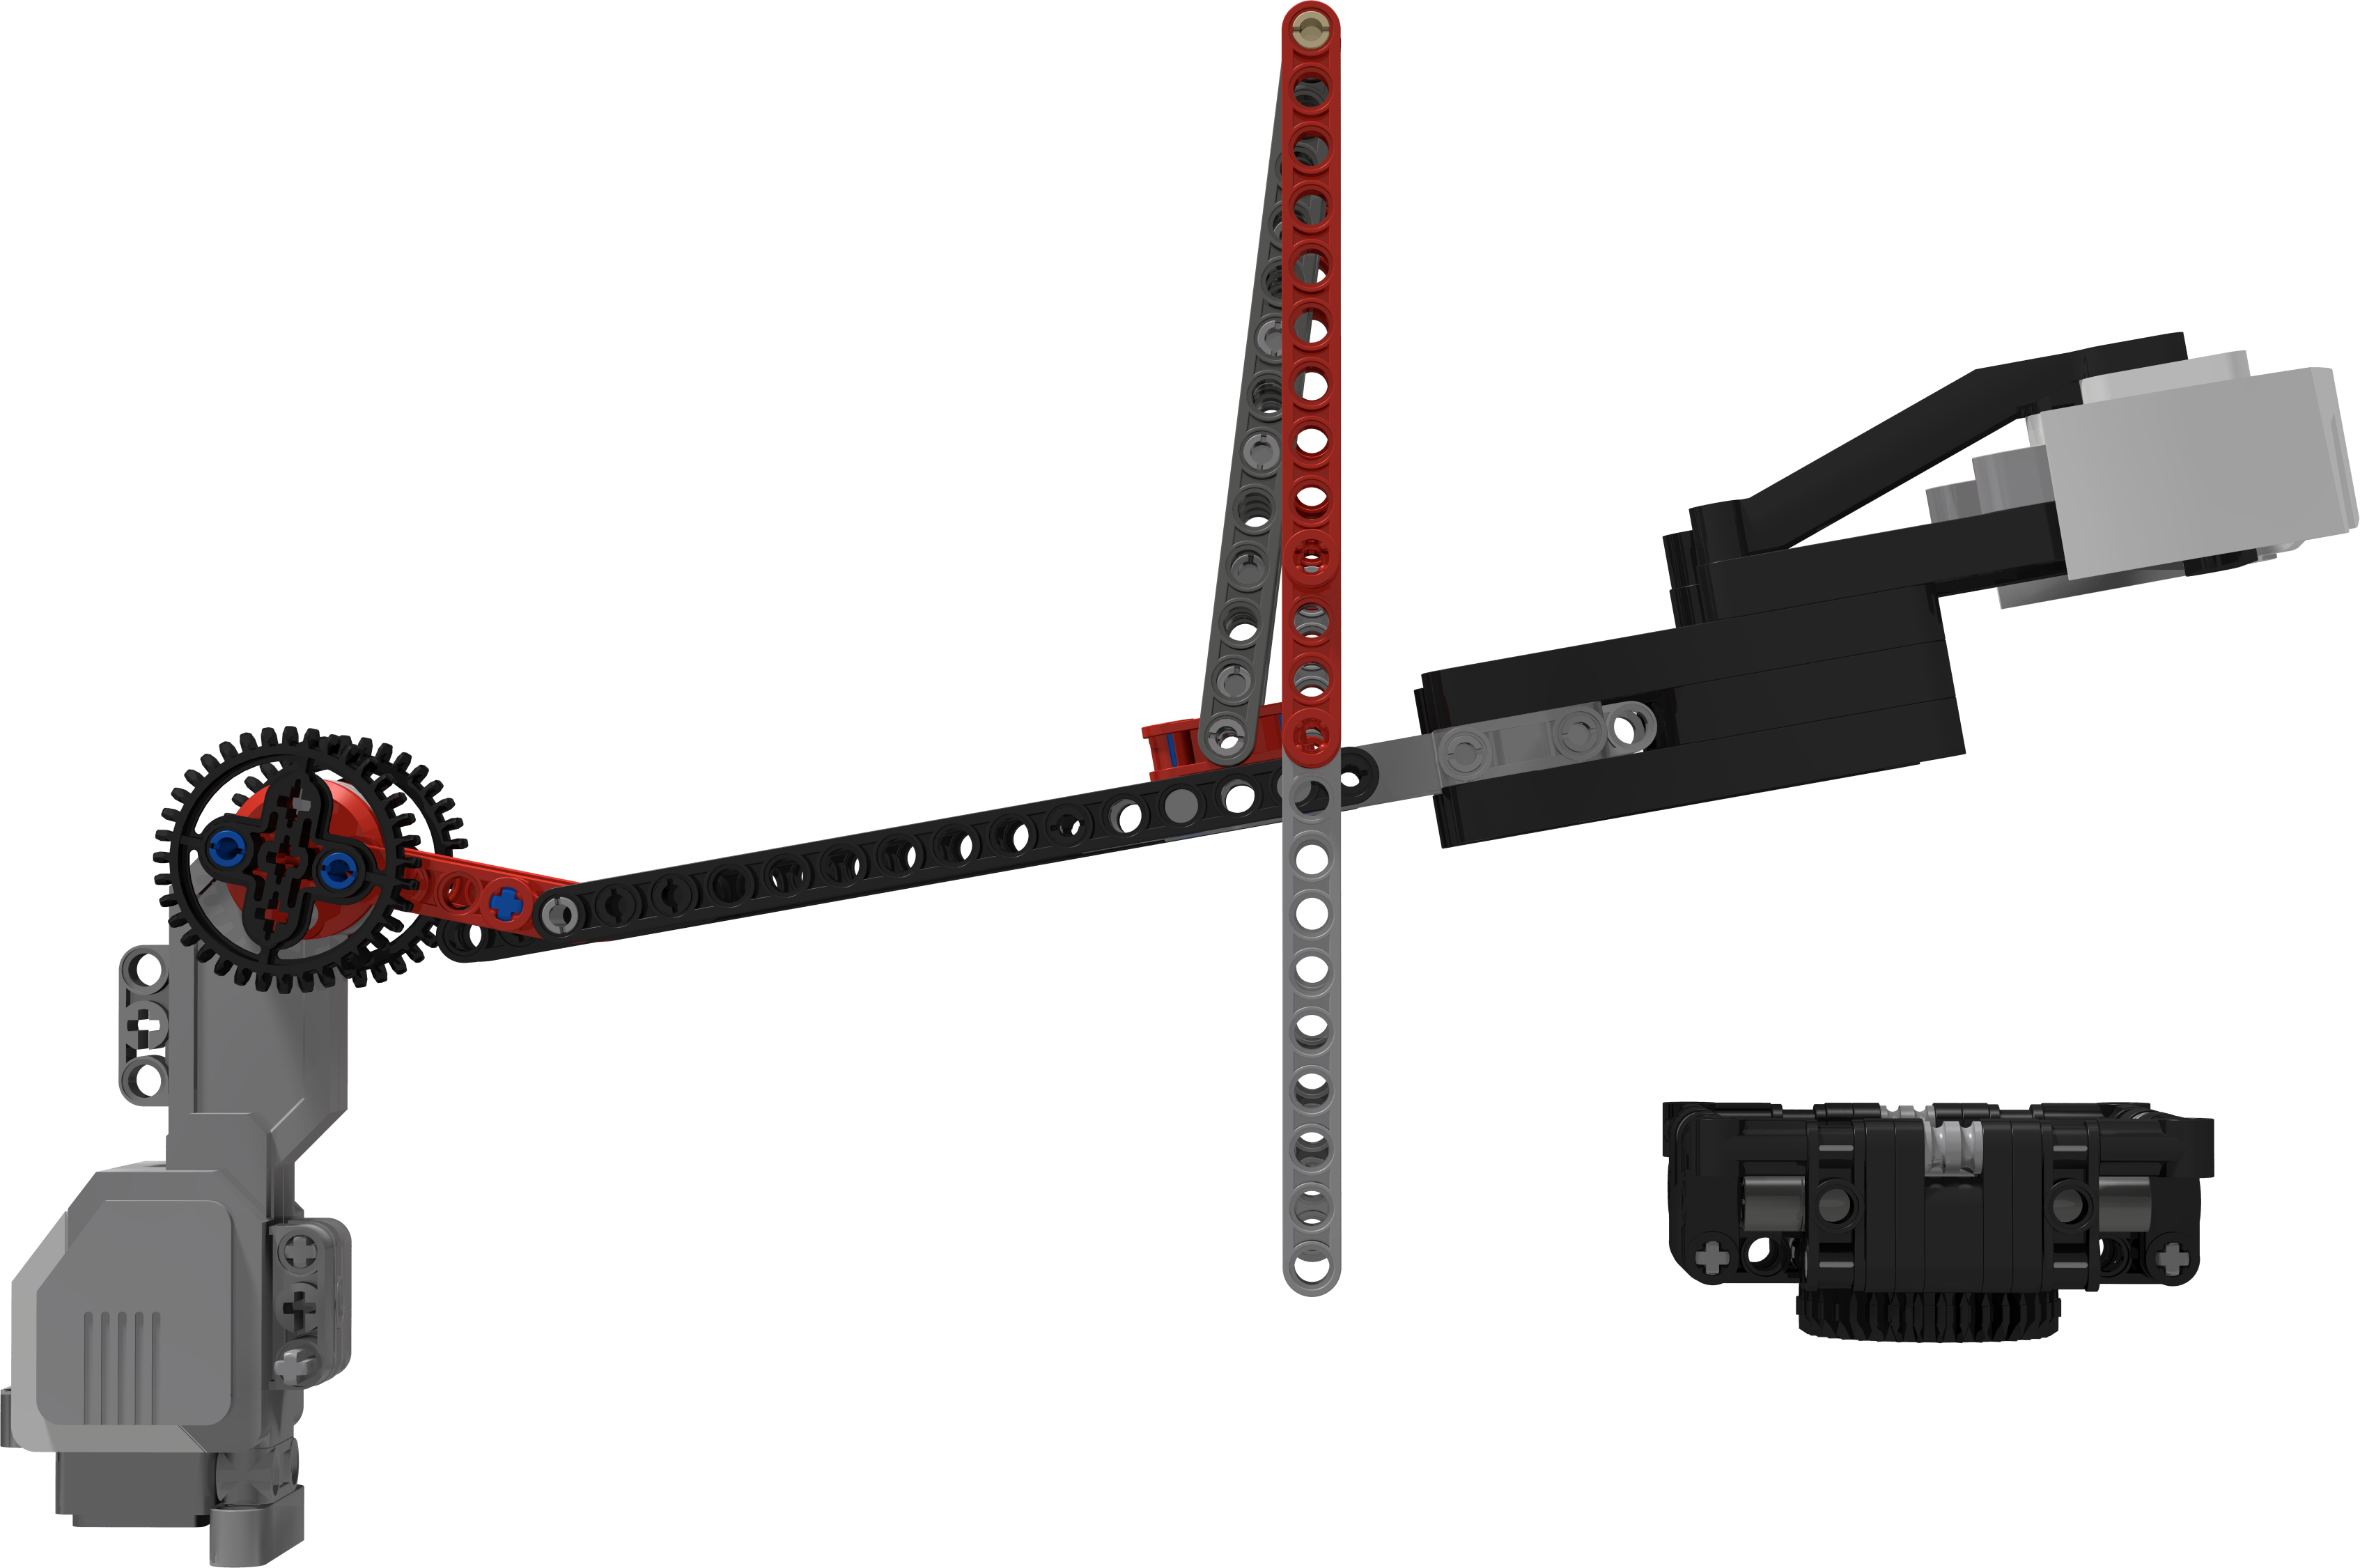
\includegraphics[width=\textwidth]{Resources/Images/rdrXMoveArmPostPush.png}
    		\caption{}
    		\label{fig:rdrXMoveArmPostPush}
    	\end{subfigure}
    	\hspace{10mm}
    	\begin{subfigure}[b]{0.25\textwidth}
    		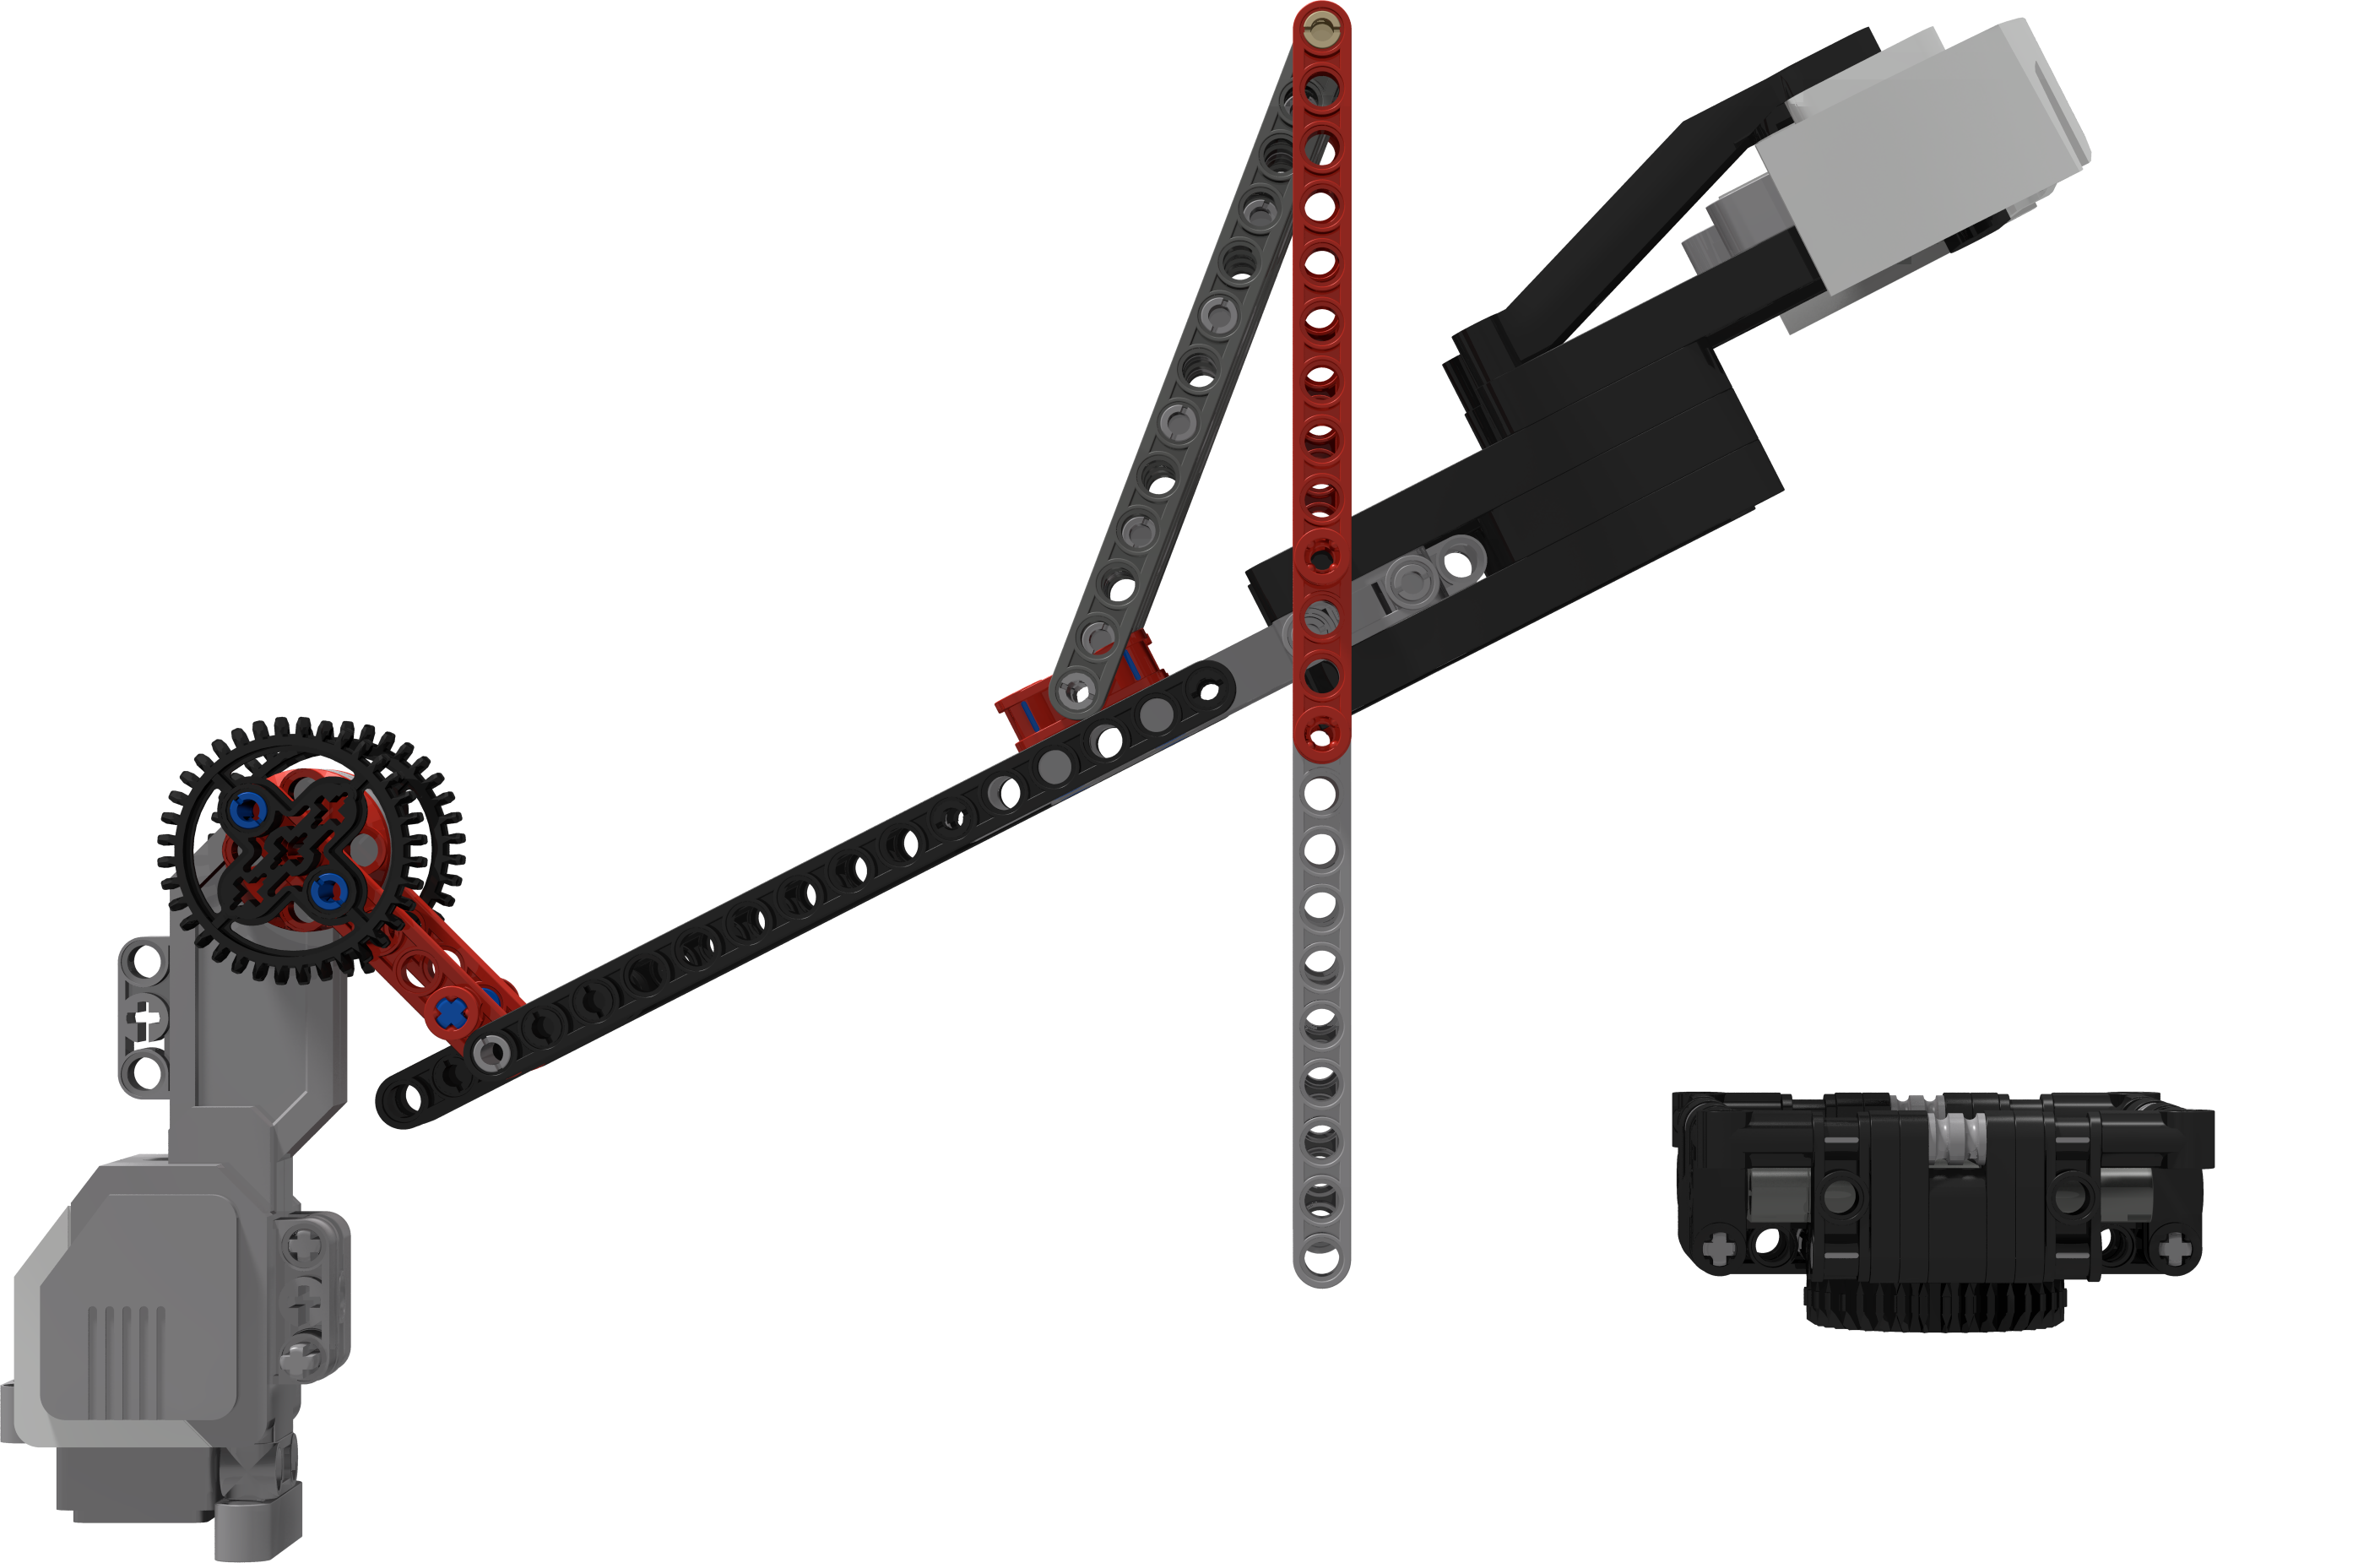
\includegraphics[width=\textwidth]{Resources/Images/rdrXMoveArmRaised.png}
    		\caption{}
    		\label{fig:rdrXMoveArmRaised}
    	\end{subfigure}
    	\caption{The steps of an \move{x}, in order}
    	\label{fig:rdrXMoveRenders}
    \end{figure}
    
    
    \subsection{Colour Sensor}
    
    The colour sensor was undoubtedly the most successful component of the MkI, and very little has been changed between design iterations. The clutch gear \legopiece{60c01} used in preventing any damage to the motor of the MkI framework actually became a hindrance: if the assembly encountered any resistance when moving (e.g. when the rack moves onto the second worm gear), then the clutch would slip and then the whole assembly would be out of line. This rarely caused incorrect scanning results, however it is easier to restrict damage by following good coding practices - which were developed with the use of the MkI - than with the clutch gear.
    
    \subsection{Full Model}
    
   	\begin{figure}[H]
    	\centering
   		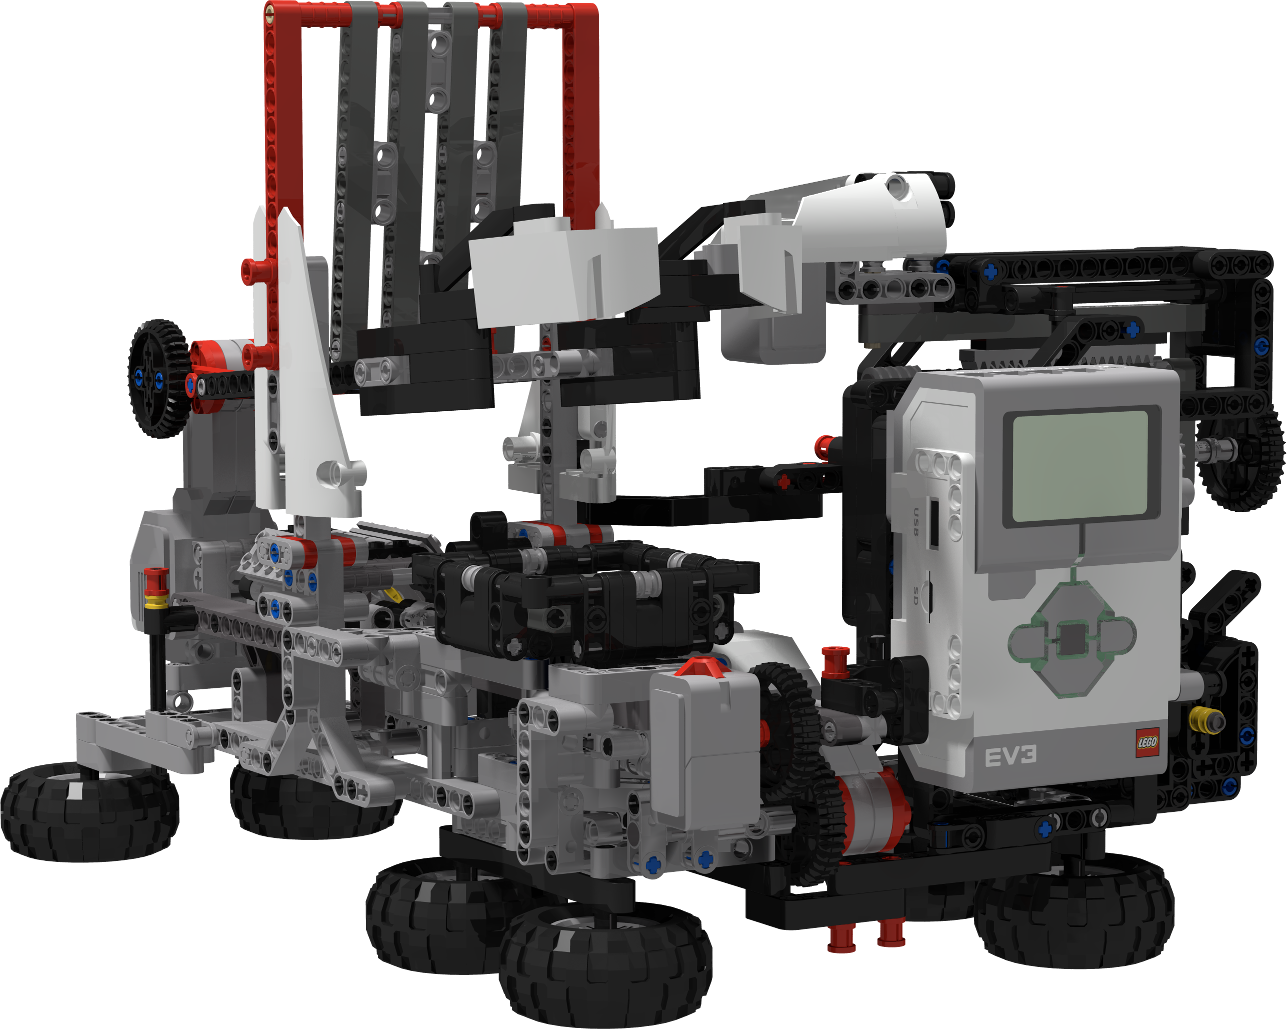
\includegraphics[width=0.9\textwidth]{Resources/Images/rdrMkIIFull.png}
   		\caption{The full MkII robot assembly}
   		\label{fig:rdrMkIIFull}
    \end{figure}
    
    Figure \ref{fig:rdrMkIIFull} is the full assembly of the MkII. As with the full render of the MkI, the model has been updated to reflect any modifications made during the building process. The construction of the MkII is of much higher quality, with fewer short-cuts and workarounds used to make up for missing pieces. It is also considerably larger than the MkI due to the increased size of the \move{x} arm. The extended framework initially caused some flexing across the body of the MkII simply due to its size and the forces exerted by the movement of the \move{x} arm. A very simple solution to this was to mount the entire MkII on \enquote{feet} made from wheels. The flexibility of the tyres allows the feet to act as dampers for the \move{x} arm, and the high friction between the tyres and the surface they sit on means that the MkII will not move around. The framework which the EV3 control brick is mounted on is actually mostly the same design as the MkI: this was one part there truly were no issues with. Reusing the framework meant less time had to be spent on the more mundane parts of the build, and more time could be spent getting the core components right. Once again, the touch sensor has been mounted on the front of the robot for easy access at runtime.
    
    \begin{figure}[H]
    	\centering
    	\begin{subfigure}[b]{0.275\textwidth}
    		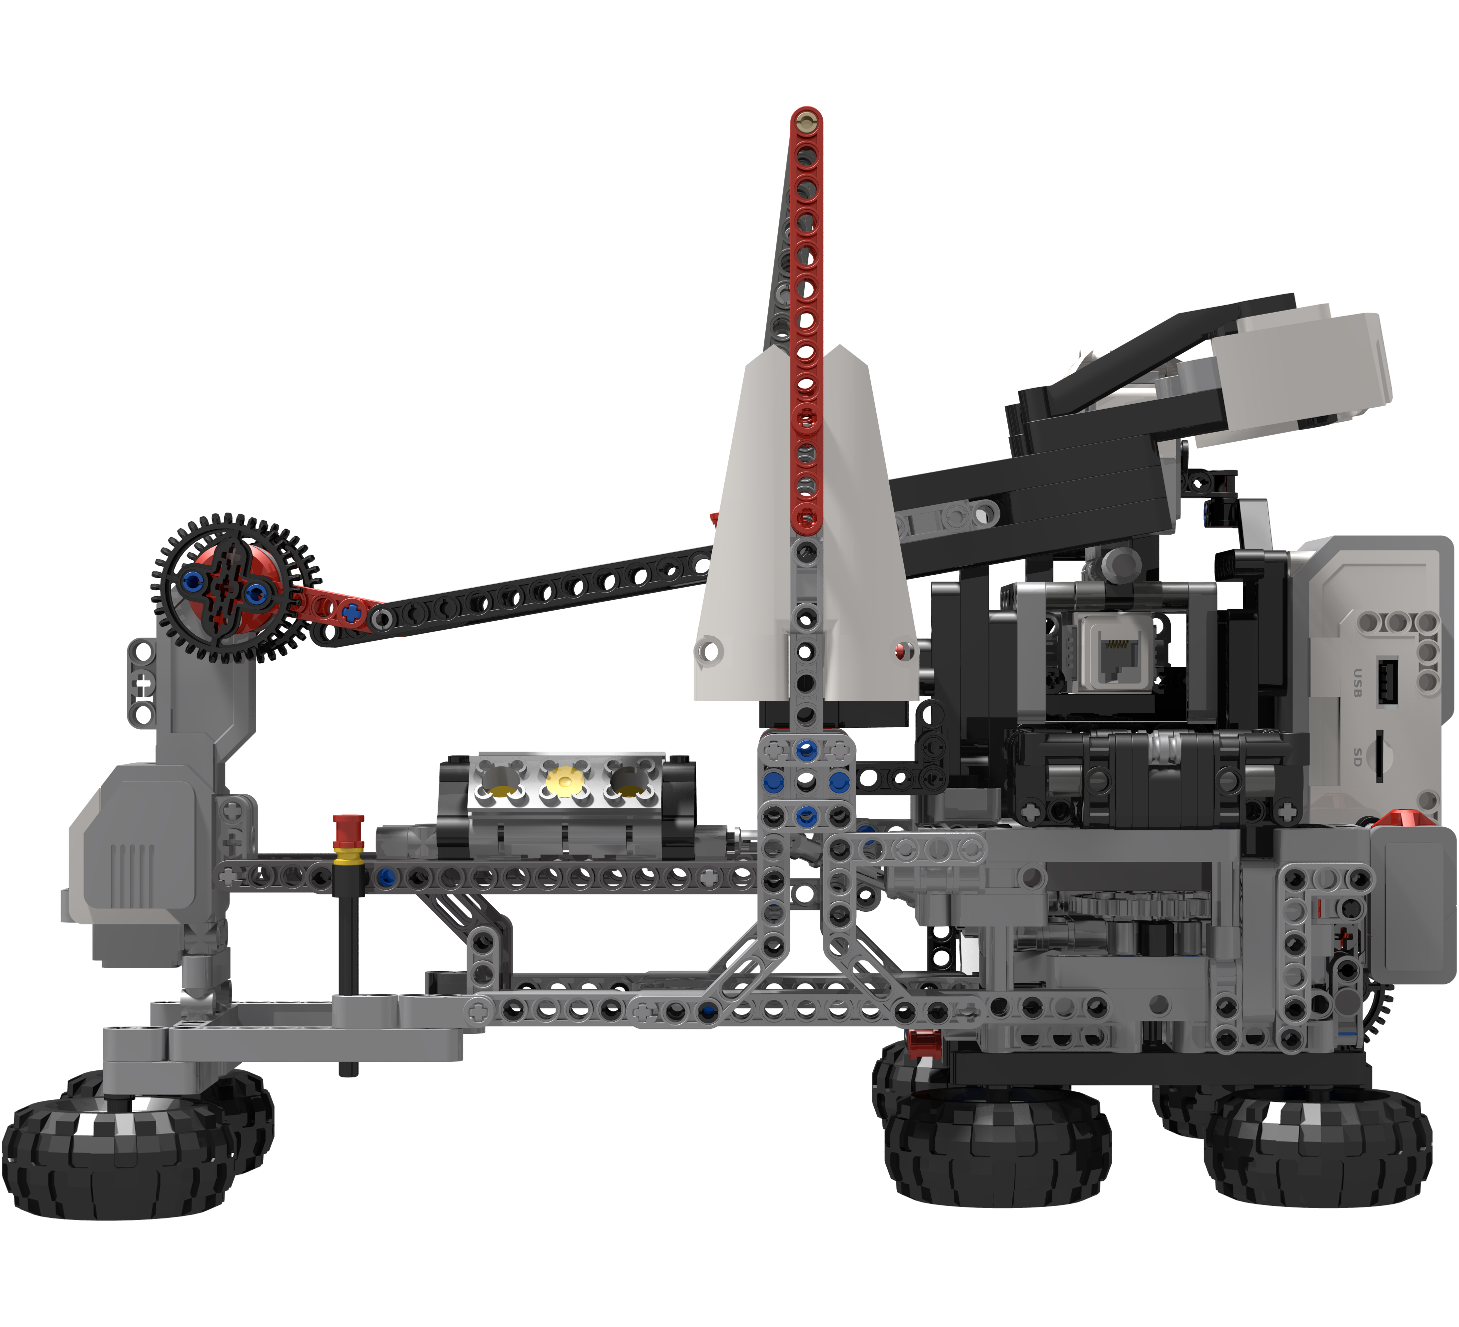
\includegraphics[width=\textwidth]{Resources/Images/rdrMkIIElevation1.png}
    		\caption{}
    		\label{fig:rdrMkIIElevation1}
    	\end{subfigure}
    	\hspace{10mm}
    	\begin{subfigure}[b]{0.275\textwidth}
    		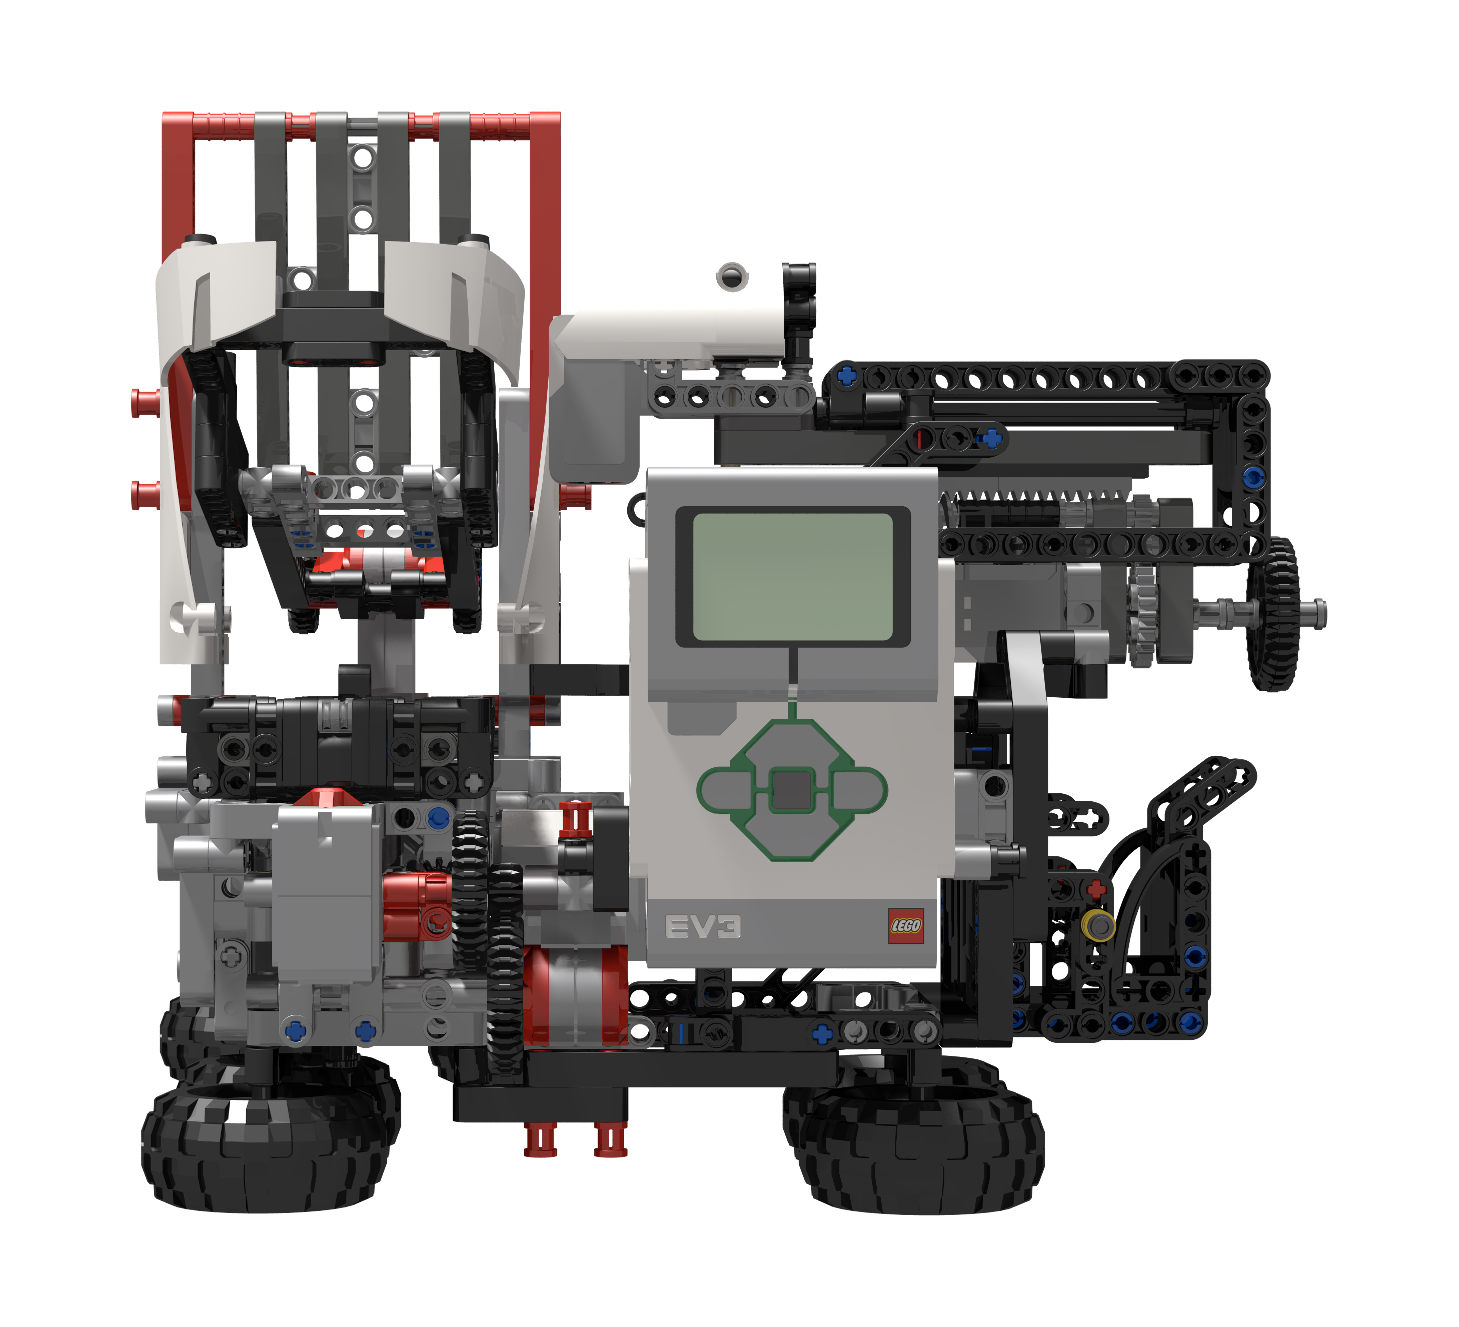
\includegraphics[width=\textwidth]{Resources/Images/rdrMkIIElevation2.png}
    		\caption{}
    		\label{fig:rdrMkIIElevation2}
    	\end{subfigure}
    	\hspace{10mm}
    	\begin{subfigure}[b]{0.275\textwidth}
    		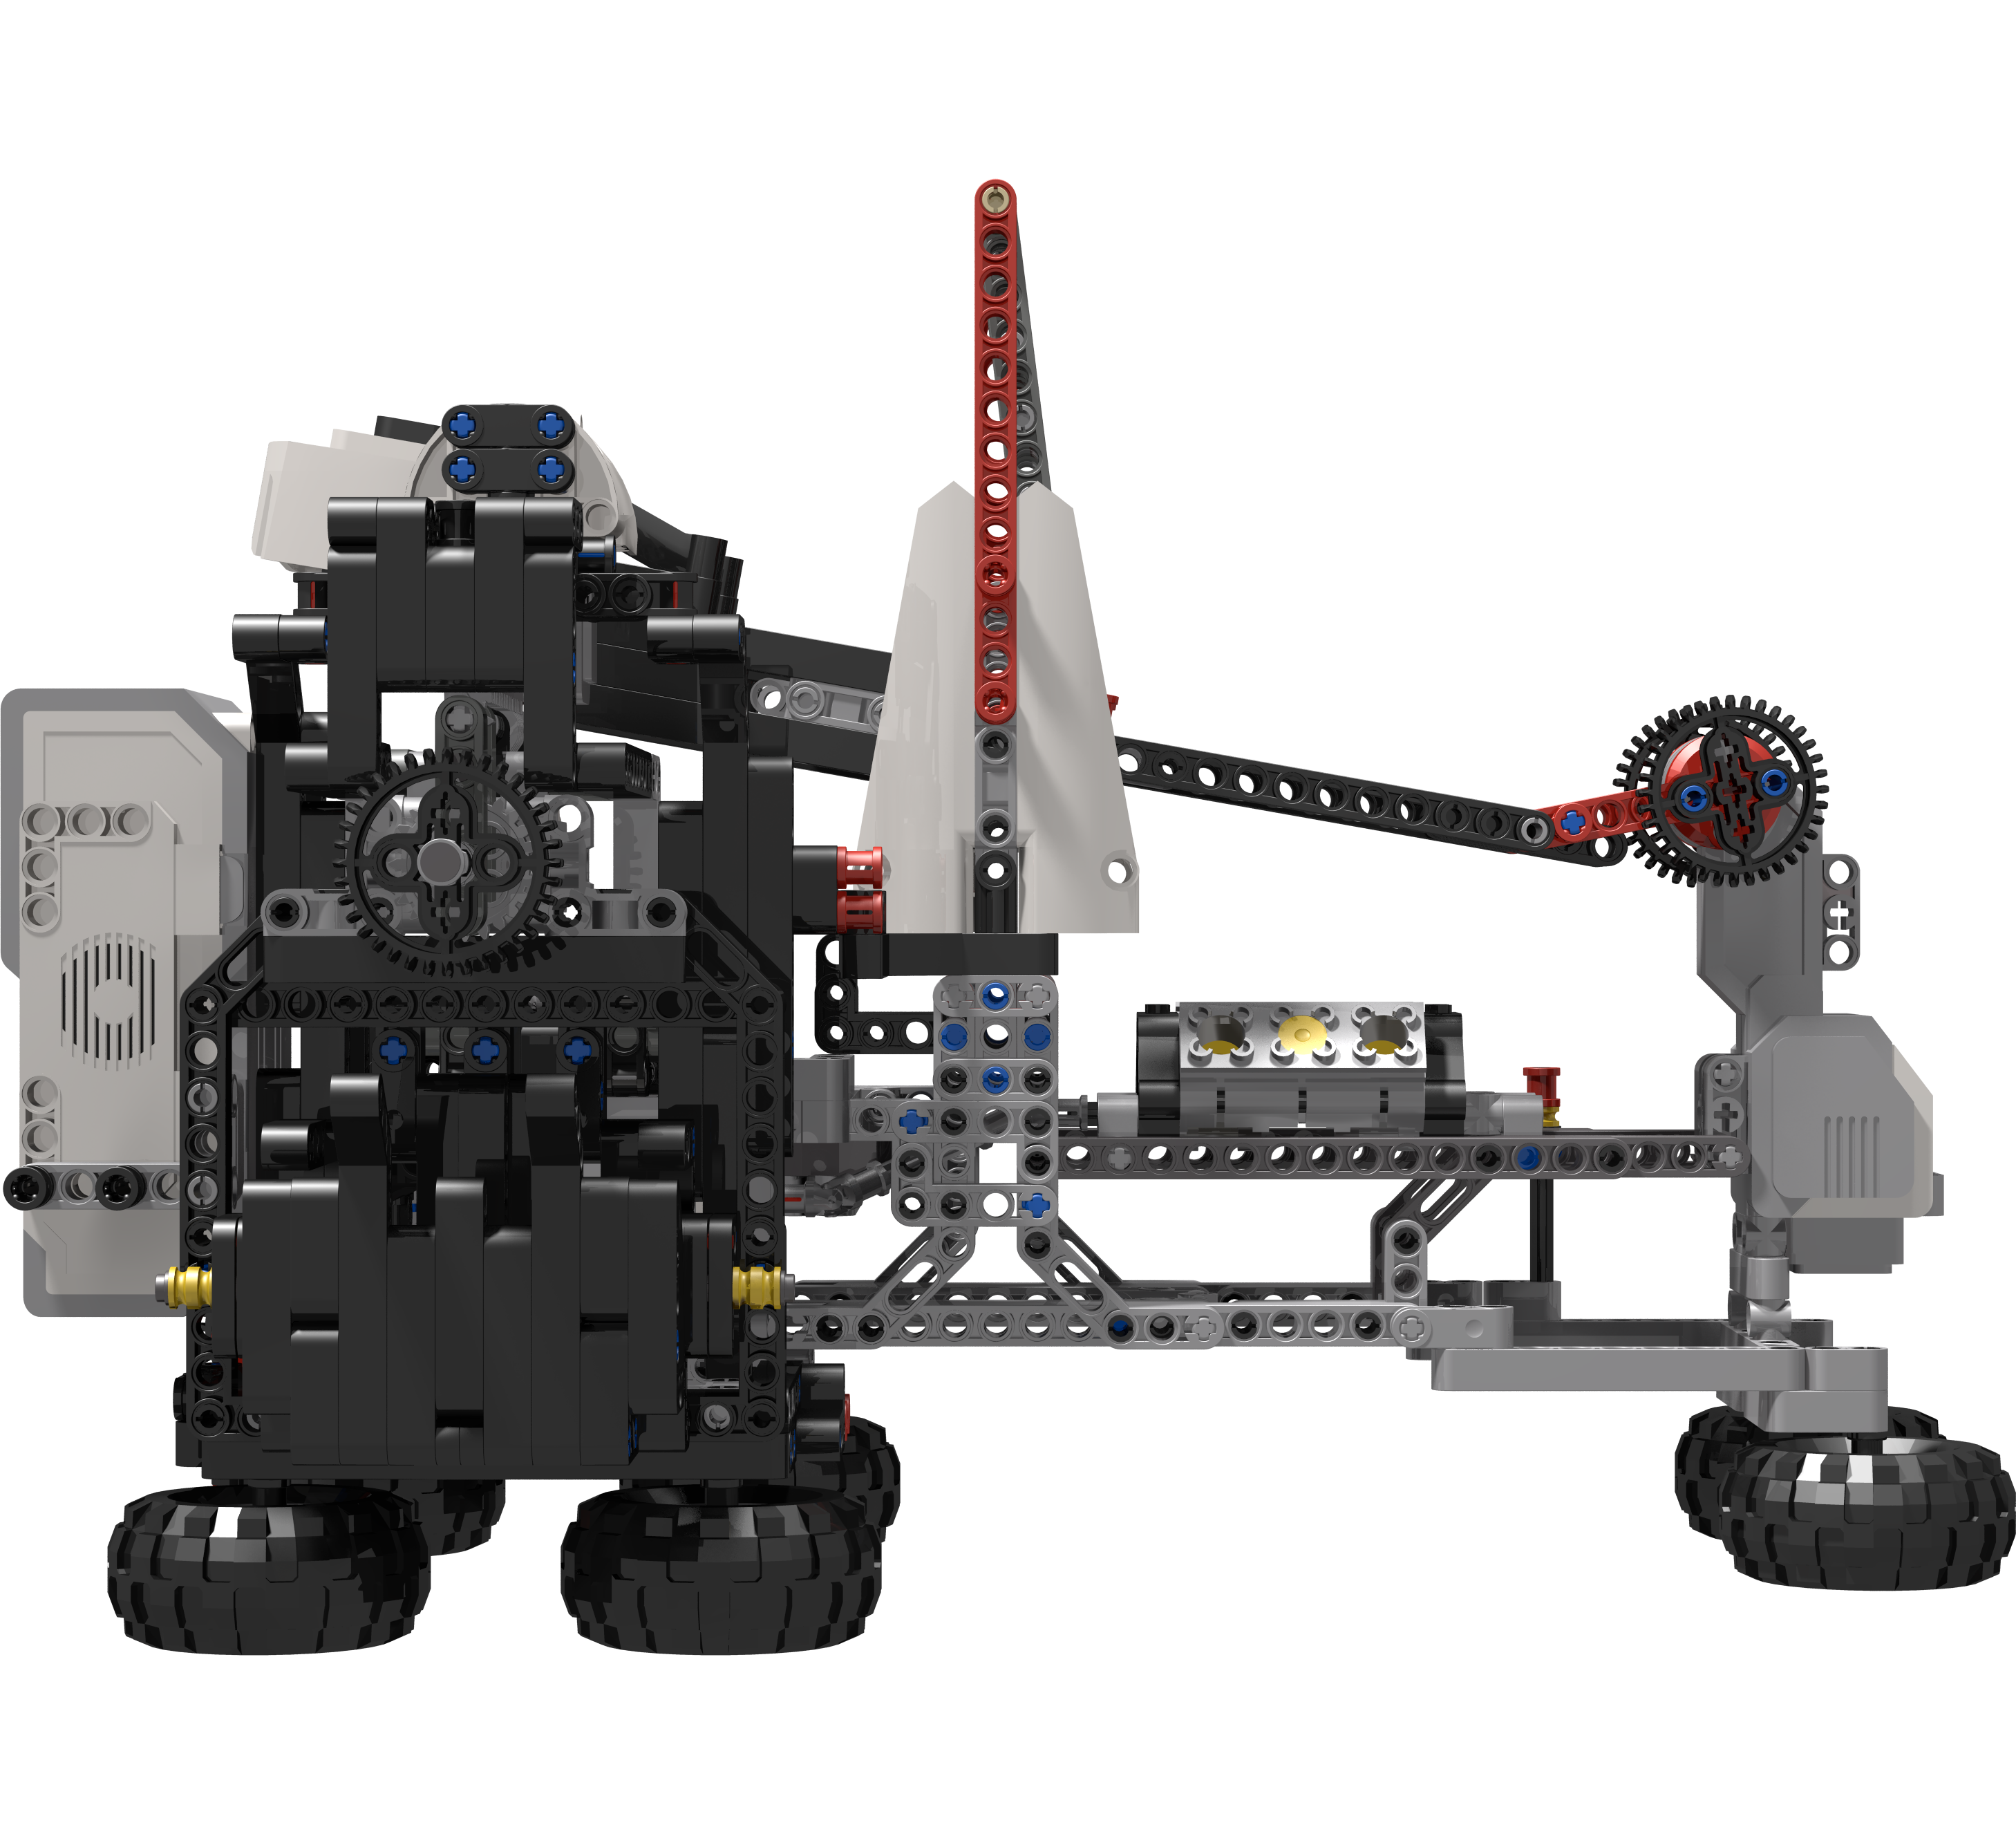
\includegraphics[width=\textwidth]{Resources/Images/rdrMkIIElevation3.png}
    		\caption{}
    		\label{fig:rdrMkIIElevation3}
    	\end{subfigure}
    	\begin{subfigure}[b]{0.275\textwidth}
    		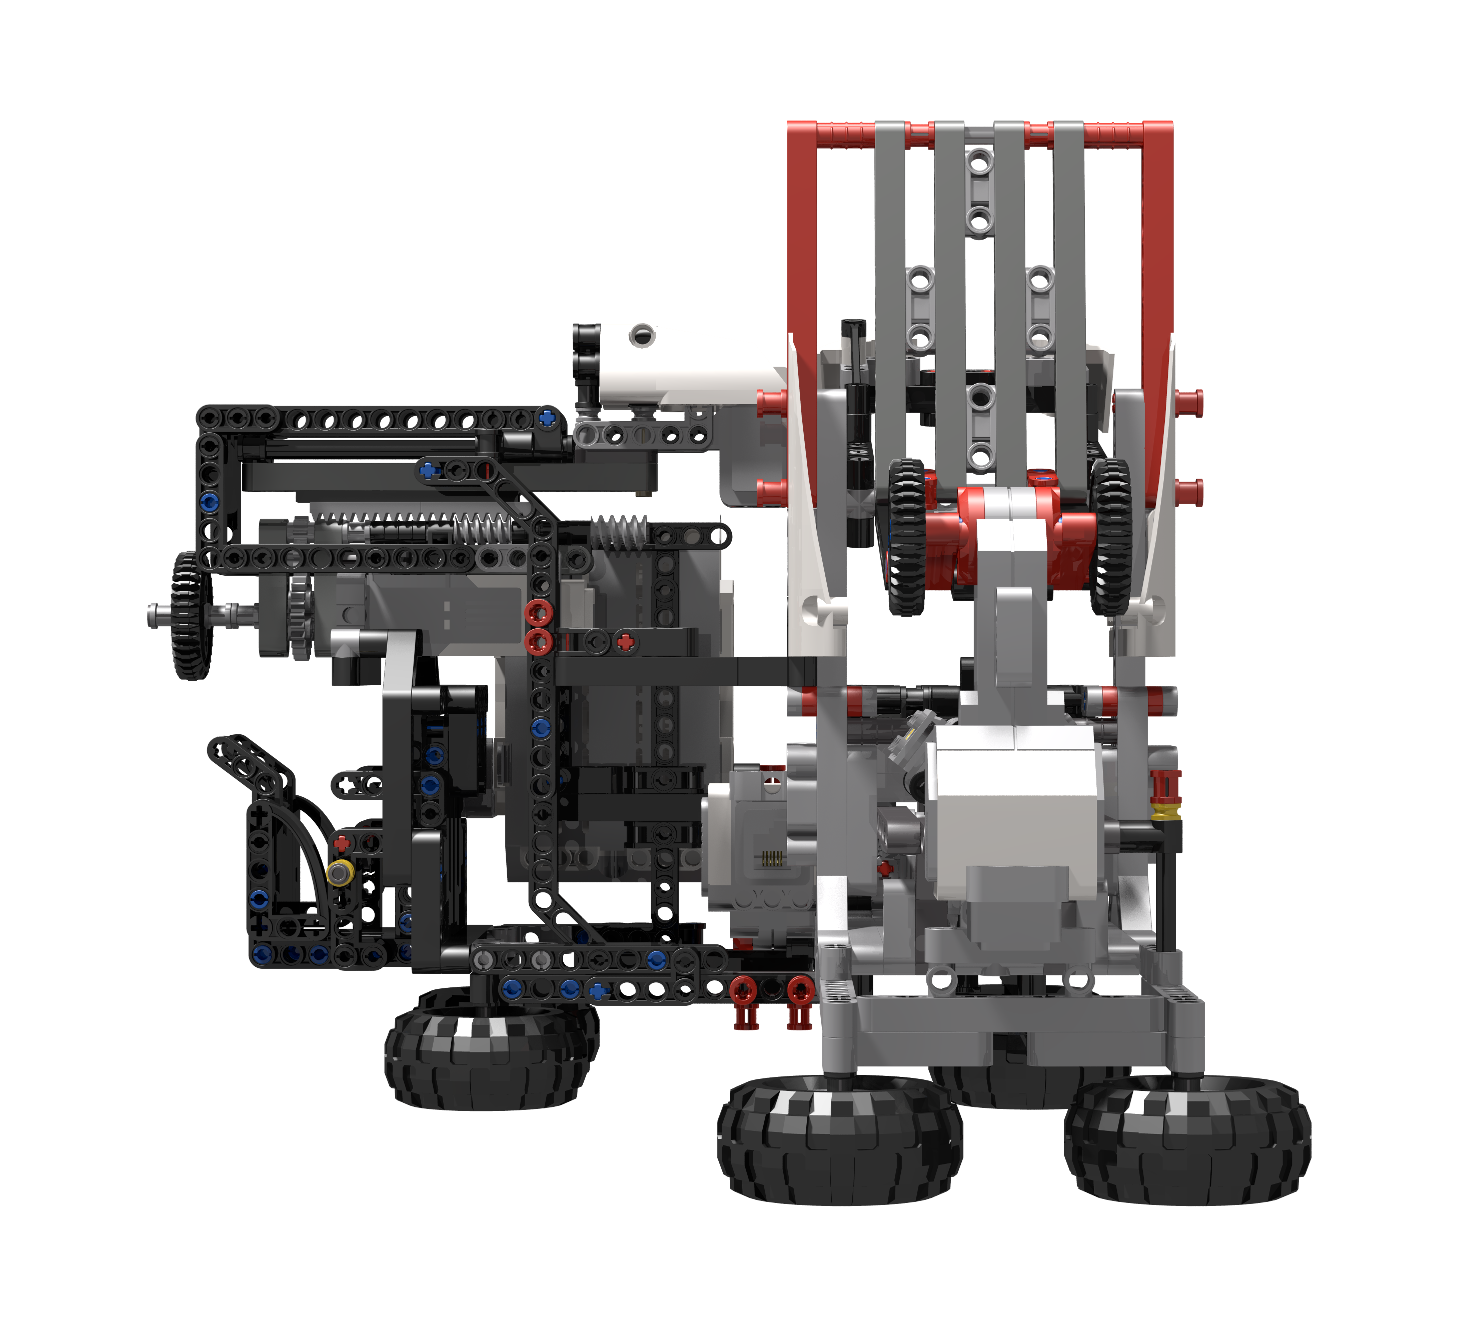
\includegraphics[width=\textwidth]{Resources/Images/rdrMkIIElevation4.png}
    		\caption{}
    		\label{fig:rdrMkIIElevation4}
    	\end{subfigure}
    	\hspace{10mm}
    	\begin{subfigure}[b]{0.275\textwidth}
    		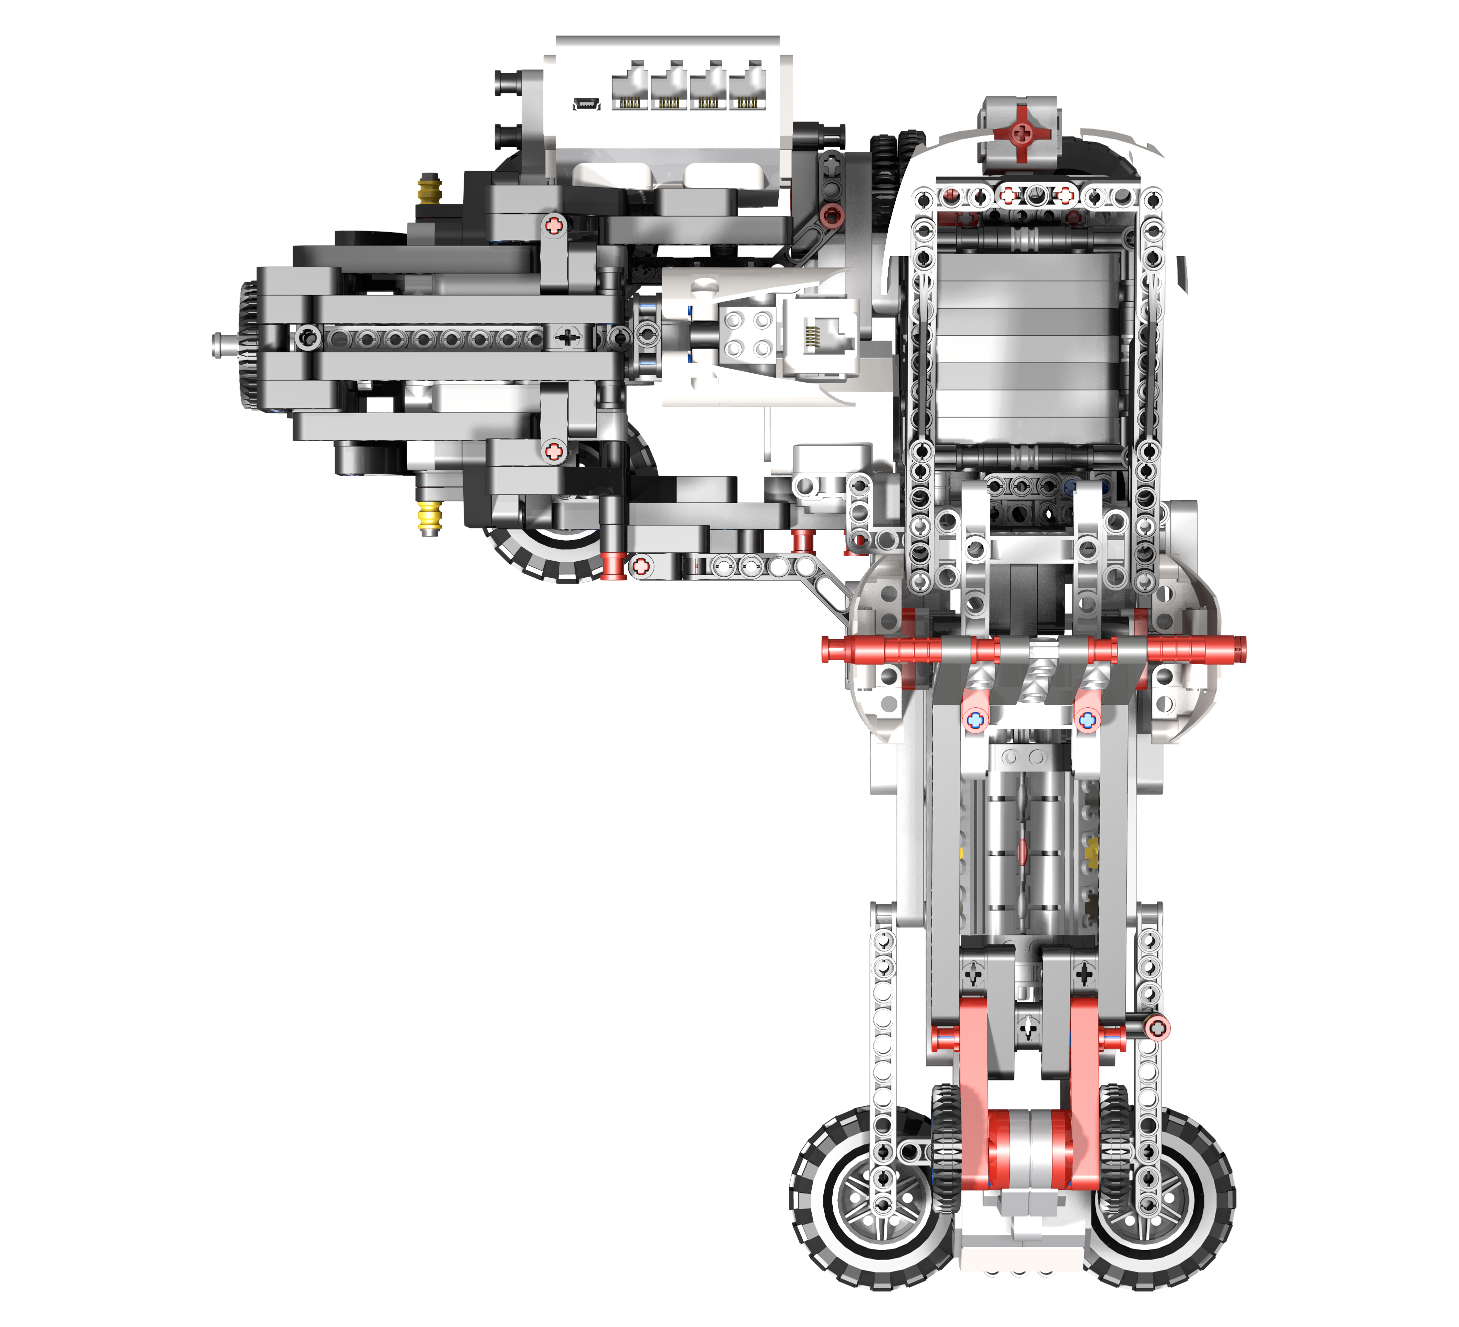
\includegraphics[width=\textwidth]{Resources/Images/rdrMkIIElevation5.png}
    		\caption{}
    		\label{fig:rdrMkIIElevation5}
    	\end{subfigure}
		\hspace{10mm}
		\begin{subfigure}[b]{0.275\textwidth}
			\includegraphics[width=\textwidth]{Resources/Images/rdrMkIIElevation6.png}
			\caption{}
			\label{fig:rdrMkIIElevation6}
		\end{subfigure}
    	\caption{Elevation and plan views of the MkII}
    	\label{fig:rdrMkIIElevations}
    \end{figure}

    \subsection{Implementation and Testing}
    
	The implementation/building process of the MkII was fairly straightforward following the MkI's implementation. The more common errors and weaknesses in the design were easier to spot, and the knowledge gained from the previous design iteration greatly aided in making the MkII an all-round strong design. The use of the spiral model in designing the robot has generated a clear process from the design stage through to the testing stage, producing a robot with very few, if any, hardware-based bugs or issues.
	
	Each of the original fundamental definitions have been followed in the design of the robot, through thorough consideration of hardware capabilities and leaving plenty of room for improvement with both hardware and software. The MkI did not achieve items Cradle \ref{lst:cr2} and \ref{lst:cr3}, and \move{x} Arm \ref{lst:x2} so these were the largest changes as the spiral model progressed. The MkII, however, has successfully fulfilled all of the definitions with a very small margin of error. It has therefore been marked as a success, and will not be developed further.
    
    \newpage
    
    \chapter[Design, Implementation and Testing: The Codebase]{Design, Implementation \\ and Testing: The Codebase}
    \epigraph{There are two ways of constructing a software design: One way is to make it so simple that there are obviously no deficiencies, and the other way is to make it so complicated that there are no obvious deficiencies. The first method is far more difficult.}{C.A.R. Hoare \cite{Hoare1981}}
    
    \section{Introduction}
    
	This is the second of the two chapters on the Design, Implementation and Testing of the project. This chapter covers the methods used, code written, and algorithms implemented to solve a Cube with the robot built in Chapter \ref{chp:designRobot}. Three main methods were implemented, with varying degrees of success, and will be discussed in their own sections. Prior to the details of the solve methods, the general structure of the software is explained to aid in understanding the methods' advantages and disadvantages.
    
    Special semantics are used in this chapter to denote move sequences and sets. A glossary is available on page \pageref{tab:abbrev}.
    
    \section{Software Flow}
    
    The general outline of the software is shown in Figure \ref{fig:flwBasic}. Regarding the decision \enquote{Is Cube valid?}, the most thorough method of validating a Cube is to check each individual cubie for correctness and validity - for this purpose, this is unnecessary because an invalid Cube is outside the parameters of the project's objectives. The validation used after scanning the Cube is simply to check the right number of colours have been scanned to double check there were no issues with the colour sensor. If the Cube is invalid, it will only be rescanned once: after the second attempt, an invalid Cube will be rejected so that the program avoids becoming caught in an infinite loop.
    
    \begin{figure}[h]
    	\centering
    	\begin{tikzpicture}[node distance=1.5cm]
	    	\node (start) [startstop] {Start};
	    	\node (ioScanCube) [io, below of=start] {Scan Cube's Position};
	    	\node (decValidCube) [decision, below of=ioScanCube, yshift=-1cm] {Is Cube valid?};
	    	\node (decFirstScan) [decision, right of=decValidCube, xshift=3cm] {Is this the first scan?};
	    	\node (proGenSolve) [process, left of=decValidCube, xshift=-3cm] {Generate solve sequence};
	    	\node (ioApplySolve) [io, below of=proGenSolve] {Apply solve sequence to Cube};
	    	\node (exitSuccess) [startstop, below of=ioApplySolve] {Exit};
	    	\node (exitFail) [startstop, below of=decFirstScan, yshift=-1.5cm] {Raise InvalidCubeError};
	    	
	    	\draw [arrow] (decValidCube) -- node[anchor=south] {No} (decFirstScan);
	    	\draw [arrow] (start) -- (ioScanCube);
	    	\draw [arrow] (ioScanCube) -- (decValidCube);
	    	\draw [arrow] (decFirstScan) |- node[anchor=south] {Yes} (ioScanCube);
	    	\draw [arrow] (decValidCube) -- node[anchor=south] {Yes} (proGenSolve);
	    	\draw [arrow] (proGenSolve) -- (ioApplySolve);
	    	\draw [arrow] (ioApplySolve) -- (exitSuccess);
	    	\draw [arrow] (decFirstScan) -- node[anchor=west] {No} (exitFail);
    	\end{tikzpicture}
    	\caption{Flowchart to show the processing in the software}
    	\label{fig:flwBasic}
    \end{figure}
    
    \section{Device-Specific Software}
    
    The hardware capabilities of the EV3 control brick are perfectly adequate for controlling the EV3's sensors and actuators, performing non-processor intensive tasks, and managing wireless connections. However, it is absolutely inadequate for solving a Cube: one of the computers used by Richard Korf to generate a solution had an (at best) 167 \si{\mega\hertz} processor, with 64 \si{\mega\byte} of RAM, and he gave estimates of four weeks to search to \depth{18} \cite{Korf1997}. The control brick has a 300 \si{\mega\hertz} processor and 64 \si{\mega\byte} of RAM - not much better than Korf's computer from 1997. The computer  that is being used for developing this project (referred to as the DevPC) has a 3.6 \si{\giga\hertz} processor and 32 \si{\giga\byte} of RAM, meaning that the processing will be performed much quicker on it than on the EV3. If both the EV3 and the DevPC are to be used, two programs which connect to each other need to be written.
    
    Python's \propernoun{socket} module is used to connect the two programs: the DevPC creates a socket and binds it to a set port on its local IP address to listen for connections, and the program waits until a device connects; the EV3 creates a socket and attempts to connect to a hard-coded constant IP address. The methods used to establish the connection both return a connection object, which can be used to send and receive data at any point in the program. The sockets can be run asynchronously, but there is no advantage to this as there are no processes which can be run concurrently in the software, as shown above.
    
    With the introduction of a second program, the flow chart in Figure \ref{fig:flwBasic} has been updated to reflect this in Figure \ref{fig:flwTwoPrograms} (overleaf). The flowchart is divided into the processes performed by the EV3 and those performed by the DevPC. The first process on each side is \enquote{Connect to [other device]}: to be accurate, these should be followed by a decision to check if the connection has been completed successfully, and if not, the chart should go back to the connection process. This has been omitted to avoid overcomplicating the diagram, and can be assumed to be in place on both sides.
    
    One of the processes added to this flowchart that was omitted from Figure \ref{fig:flwBasic} is \enquote{Translate solve sequence}. This is a vital step in solving a Cube with a \lego Robot, and is explained below.
    
	\begin{figure}[h!]
    	\centering
    	\begin{tikzpicture}[node distance=1.5cm]
	    	\node (dividerStart) {};
    	
	    	\node (startEV3) [startstop, left of=dividerStart, xshift=-5.5cm, yshift=-1cm] {EV3};
	    	\node (proConnectDevPC) [process, below of=startEV3] {Connect to DevPC};
	    	\node (ioScanCube) [io, below of=proConnectDevPC] {Scan Cube's Position};
	    	\node (decValidCube) [decision, below of=ioScanCube, yshift=-1cm] {Is Cube valid?};
	    	\node (decFirstScan) [decision, right of=decValidCube, xshift=2.5cm] {Is this the first scan?};
	    	\node (stopEV3Fail) [startstop, below of=decFirstScan, yshift=-1.25cm] {Raise InvalidCubeError};
	    	\node (ioTransmitCube) [io, below of=decValidCube, yshift=-2.75cm] {Transmit Cube position};
    		\node (ioReceiveSolve) [io, below of=ioTransmitCube, yshift=-3cm] {Receive solve sequence};
    		\node (proPerformSolve) [process, below of=ioReceiveSolve] {Perform solve sequence on Cube};
    		\node (stopEV3) [startstop, below of=proPerformSolve] {Stop EV3};
	    	
	    	\node (startDevPC) [startstop, right of=dividerStart, xshift=1.5cm, yshift=-1cm] {DevPC};
	    	\node (proConnectEV3) [process, below of=startDevPC] {Connect to EV3};
	    	\node (ioReceiveCube) [io, below of=proConnectEV3, yshift=-6.75cm] {Receive Cube position};
	    	\node (proGenerateSolve) [process, below of=ioReceiveCube] {Generate solve sequence};
	    	\node (proTranslateSolve) [process, below of=proGenerateSolve] {Translate solve sequence};
	    	\node (ioTransmitSolve) [io, below of=proTranslateSolve] {Transmit solve sequence};
	    	\node (stopDevPC) [startstop, below of=ioTransmitSolve, yshift=-1.5cm] {Stop DevPC};
    		
    		\node (dividerEnd) [below of=dividerStart, yshift=-17.5cm] {};
    	
    		\draw [line] (dividerStart) -- (dividerEnd);
    		
    		\draw [arrow] (startEV3) -- (proConnectDevPC);
    		\draw [arrow] (proConnectDevPC) -- (ioScanCube);
    		\draw [arrow] (ioScanCube) -- (decValidCube);
    		\draw [arrow] (decValidCube) -- node[anchor=south] {No} (decFirstScan);
    		\draw [arrow] (decFirstScan) |- node[anchor=south] {Yes} (ioScanCube);
    		\draw [arrow] (decFirstScan) -- node[anchor=west] {No} (stopEV3Fail);
    		\draw [arrow] (decValidCube) -- node[anchor=east] {Yes} (ioTransmitCube);
    		\draw [arrow] (ioReceiveSolve) -- (proPerformSolve);
    		\draw [arrow] (proPerformSolve) -- (stopEV3);

    		\draw [arrow, dashed] (ioTransmitCube) -- (ioReceiveCube);
    		\draw [arrow, dashed] (ioTransmitSolve) -- (ioReceiveSolve);
    	
    		\draw [arrow] (startDevPC) -- (proConnectEV3);
    		\draw [arrow] (ioReceiveCube) -- (proGenerateSolve);
    		\draw [arrow] (proGenerateSolve) -- (proTranslateSolve);
    		\draw [arrow] (proTranslateSolve) -- (ioTransmitSolve);
    		\draw [arrow] (ioTransmitSolve) -- (stopDevPC);
    	\end{tikzpicture}
    	\caption{The EV3 and DevPC work synchronously but separately}
    	\label{fig:flwTwoPrograms}
    \end{figure}
    
    \section{Move Sequence Translation}
    
    The algorithms considered and discussed in the Literature Review (as well as others used in determining God's Number) are designed to work with a standard moveset \moveset{L.R.U.D.F.B} (as well as half turns and counter-clockwise turns). The design of the robot means that it is restricted to the moveset \moveset{X.Y.y'y2D.d'd"} - and will therefore require any incompatible sequences to be translated to the robot's moveset.
    
    When the entire Cube is rotated, the \tit{colour} of the faces will change but the faces' \tit{orientations} will not (analogous to when one turns on the spot: left and right have changed, but east and west have not). This means that the frame of reference for the moves will have to remain invariant throughout a sequence by compensating for any full Cube rotations.
    
    This is best explained with an example: the first step in performing the sequence \movesequence{u.f} would be to do perform \movesequence{x2d} in order to complete the \move{u}; but now that the original \face{f} has moved (due to the \movesequence{x"}) - it must be located, the Cube must be rotated to get the original \face{f} into the cradle, and then the sequence can be completed. The simplest method of overcoming this complication is to convert the original move sequence to an equivalent sequence of colour-based moves: \movesequence{u.f} $\equiv$ \movesequence{W.G}.
    
    Once the original sequence has been converted to a colour-based sequence, a deep copy of the original Cube is made and the coloured sequence is iteratively translated and applied to this Cube. On each element of the sequence, the colour is converted back to a face move (allowing preservation of the correct frame of reference). Once this new face-based move is found, it is converted to a short move sequence that will move the face into the cradle and rotate the face correctly to match the original move. This short sequence comprises moves compatible with the robot.
    
    Each of the moves in the short sequence is applied to the copied Cube, and appended to a list of moves which is returned once the original sequence is processed. The application of the moves to the Cube allows following moves to be translated correctly (as the Cube will have changed orientation in real life so needs to in this simulation). Continuing the previous example of \movesequence{u.f}, the translation is written below. Colours are underlined and the output sequence is emboldened for clarity:
    \begin{align*}
    \movesequence{U.F}		\;	&\rightarrow		\;	\movesequence{\tun{w}.\tun{G}}													\\
    \movesequence{\tun{w}}	\;	&\rightarrow		\;	\movesequence{U}																\\
    \movesequence{U}		\;	&\rightarrow		\;	\movesequence{X2D}	\;	\rightarrow	\;	\movesequence{\tbo{X}.\tbo{X}.\tbo{d}}	\\
    &\implies				\;	\movesequence{U.F}	\;	\rightarrow			\;	\movesequence{\tbo{X}.\tbo{X}.\tbo{d}.\tun{G}}			\\
    \movesequence{\tun{G}}	\;	&\rightarrow		\;	\movesequence{B}																\\
    \movesequence{B}		\;	&\rightarrow		\;	\movesequence{X.D}																\\
    &\implies				\;	\movesequence{U.F}	\;	\rightarrow			\;	\movesequence{\tbo{X}.\tbo{X}.\tbo{d}.\tbo{X}.\tbo{d}}
    \end{align*}
    
    This final move sequence will then be transmitted to the robot and used to control the motors to manipulate the Cube.
    
    \section{Object Classes}
    
    This project has two main object classes, which are instantiated at the start of the program and used throughout. These classes are both discussed, explained and examined below as an introduction to the methods used in solving a Cube.
    
    \subsection{Robot} \label{sec:robotObject}
    
    The first class is the \lstinline|Robot|: an object which is used to represent the real world \lego robot, provide a controller for the actuators, and read real world data using the sensors. 
    
    The \lstinline|Robot| class has one class attribute for each peripheral (sensors and actuators) to allow individual control. Upon initialisation of the \lstinline|Robot|, each peripheral's connection is checked and the motors are then manually initialised. To do this, the braking method for the motors is set to \lstinline|'coast'|, which means that all resistance is removed from the rotor and they can be turned to the correct position using the large gears shown in Figure \ref{fig:rdrInitialiser} on page \pageref{fig:rdrInitialiser}. Once the motors are initialised, the touch sensor can be pressed to continue the program: this sets the braking method of the motors to \lstinline|'hold'|, providing an active resistance to the rotors to ensure there is no unwanted rotation.
    
    The \lstinline|Robot| has a number of methods for controlling the core components: Algorithms \ref{alg:scanupface} and \ref{alg:scancube} have been implemented to scan the Cube; constant values are used to set the endpoints of an \move{x} performed by the arm; \lstinline|rotate_cradle| is a method which has an optional parameter (with a default value of 90) by which to rotate the cradle; and there are moves for each method in the set \moveset{x.x'x2y.y'y2d.d'd"} (The \move{x'} is interpreted as \movesequence{x.x.x}).
    
    \subsection{Cube}
    
    \subsubsection{The \lstinline|Cube| Class}
    
    The second object defined in the software is the \lstinline|Cube| object.  As well as the main \lstinline|Cube| class, there are four \lstinline|Enum| classes which are used in defining a \lstinline|Cube|: \lstinline|Color|, which has eight members - each representing a colour which the \lego sensor can \enquote{see} (\lstinline|NONE|, \lstinline|DARK|, \lstinline|WHITE|, \lstinline|ORANGE|, \lstinline|GREEN|, \lstinline|BLUE|, \lstinline|RED| and \lstinline|YELLOW|); \lstinline|Move|, an Enum with one member for each possible move; \lstinline|Face|, which has one member for each Cube face; and \lstinline|Rotation|, which is a simple Enum with only two members - \lstinline|CLOCKWISE| and \lstinline|COUNTER_CLOCKWISE|.
    
    To store the position of a Cube, the three-dimensional Cube is turned into a two-dimensional net, which is then turned into a single string by \enquote{reading} the facelets from top to bottom, left to right as shown in Listing \ref{lst:cubePrint}. The \lstinline|position| attribute can be accessed by calling \lstinline|Cube.position|, and a coloured net can be output by printing the \lstinline|Cube| object. A \lstinline|Cube| has two optional parameters upon initialisation. The first is the position, as a string which defaults to the solved position. The second argument is a boolean to state whether the Cube is temporary. If set to \lstinline|True|, some less commonly used attributes and methods are ignored to reduce memory usage and processing requirements. There are also six class attributes to represent the faces of the Cube. Each of these is a string of six characters, each representing the colour of a facelet when the face is \enquote{read} top to bottom, left to right.
    
    The final attribute of a Cube is \lstinline|position_reduced|: a reduced-colour version of the Cube's faces. In this version, only three colours are used, and the others are substituted for their opposite faces.
    
	\begin{lstlisting}[caption={The two different ways of accessing a Cube's position}, label={lst:cubePrint}]
    >>> from cube_class import Cube
    >>> cube = Cube()
    >>> print(cube.position)
    WWWWWWWWWOOOGGGRRRBBBOOOGGGRRRBBBOOOGGGRRRBBBYYYYYYYYY
    >>> print(cube)
          |\fw \fw \fw|
          |\fw \fw \fw|
          |\fw \fw \fw|
    |\fo \fo \fo \fg \fg \fg \fr \fr \fr \fb \fb \fb|
    |\fo \fo \fo \fg \fg \fg \fr \fr \fr \fb \fb \fb|
    |\fo \fo \fo \fg \fg \fg \fr \fr \fr \fb \fb \fb|
          |\fy \fy \fy|
          |\fy \fy \fy|
          |\fy \fy \fy|
	>>> print Cube(cube.position_reduced)
	      |\fw \fw \fw|
	      |\fw \fw \fw|
	      |\fw \fw \fw|
	|\fr \fr \fr \fb \fb \fb \fr \fr \fr \fb \fb \fb|
	|\fr \fr \fr \fb \fb \fb \fr \fr \fr \fb \fb \fb|
	|\fr \fr \fr \fb \fb \fb \fr \fr \fr \fb \fb \fb|
	      |\fw \fw \fw|
	      |\fw \fw \fw|
	      |\fw \fw \fw|\end{lstlisting}
    
    \subsubsection{Updating a \lstinline|Cube|}
    
    In order to replicate each of the twenty-seven possible moves, twenty-seven corresponding methods were created to simulate each move. They make use of the \lstinline|Cube|'s setter methods, which each take a single string as an argument and set the corresponding characters in the \lstinline|position| attribute. They also use the method \lstinline|rotate_face| which takes a direction (of type \lstinline|Rotation|) and a face (of type \lstinline|Face|) and moves the facelets \ang{90} in the given direction.
    
    To ensure that all the class attributes accurately describe the Cube's position at any given time, methods have been written to update all of the necessary attributes when the object is modified. As well as the setter methods, there are two getter methods. The first takes a keyword argument and returns a \lstinline|Color| object: the keyword is either \lstinline|'facelet'| which is an integer facelet reference, or \lstinline|'face'| to lookup that face's colour. The second getter method takes a \lstinline|Color| as an argument and returns the face which is that colour.
    
    \section{Method 1: Tree Solving} \label{sec:treeSolving}
    
    During the development of this project, three main methods of solving the Cube were implemented. Each had it's own advantages and disadvantages and are discussed in this section and the following two.
    
    \subsection{Implementation} \label{sec:treeSolveImplementation}
    
    The very first step in creating a reliable solve method was to create a reliable object class, and a data structure to store the object in. The \lstinline|Position| class defines an object with four attributes: the depth of the position; the position's string representation; the move sequence used to get to that position; and the ID of that position. Richard Korf discusses the successful implementation of a search tree and an iterative deepening A* algorithm to solve a Cube in his 1997 paper \cite{Korf1997}. 
    
   	\begin{aside}
   		    It is important to note that a lot of the research into efficient solving algorithms was done between twenty and forty years ago, and is now lost to the abandonment of websites, mailing lists, and newsletters in favour of much simpler websites and blog posts with much less information and community interaction. Some of the data from the \enquote{golden age} of solving Cube's is available as large, disorganised archives  - but a lot of it was done before the days of commonplace online interaction, and the amount of data available to assist in the design and implementation of solve methods is far more limited than is desirable if one has no contacts in the world of Rubik's Cube solving. This all means that some of the development hit a premature dead end and was abandoned in favour of attempting a larger range of methods for cross-comparison.
   	\end{aside}

    Having evaluated the available information about the use of search trees and spaces in solving a Cube, it seemed like it could actually be a fairly trivial task: use a moveset to manipulate a Cube until it is solved; a lot of positions can be eliminated through duplication checking and other optimisations; and the code to create a recursive search space will also be relatively simple. This assumption was soon proved very wrong.
    
    A dictionary was used for storing the search space, with the positions at each depth stored as the values and the depths as the keys. Inside a \lstinline|while not solved| loop, a nested \lstinline|for| loop iterated through the values in the dictionary at the previous depth, and a second nested \lstinline|for| loop applied each move in the defined moveset to each position. The only optimisations applied to the generations was the use of a set to hold the previously generated positions for duplication checking. This optimisation reduced the time required to solve a Cube at \depth{$n$} by an approximate factor of $0.45n$, and the number of positions by $0.58n$.
    
    In order to observe the progress being made by the tree generator, a graphical user interface (GUI) was created to display the time elapsed, current depth, position count and move sequence, alongside a graphical representation of the Cube. To take full advantage of Python's versatility, the \propernoun{multiprocessing} package was imported to separate the generation and GUI processes on to different cores in the computer's CPU. Multiprocessing was chosen over multithreading due to the complete separation of processes - different threads still operate on the same CPU core so don't take full advantage of a computer's processing power - and inherent increase in processing speed. Although this complete separation meant the processing speed was increased, it presented a challenge in getting the positions from the generator to the GUI across completely distinct memory locations.
    
   	\begin{figure}[H]
    	\centering
    	\includegraphics[width=0.7\textwidth]{Resources/Images/imgTreeSolveGUI}
    	\caption{The GUI to display the Tree solver's progress}
    	\label{fig:imgTreeSolveGUI}
    \end{figure}
    
    A \lstinline|LifoQueue| was used to bridge the gap between the two processes. It was used as a parameter in the creation of the two processes, providing a pointer back to its memory location whenever necessary. A \tit{LIFO} queue was used rather than a \tit{FIFO} queue because positions were generated faster than the GUI could update, causing a lag in the GUI as it worked through the ever-growing queue and reducing its effectiveness. The disadvantage of the LIFO format was that positions which were skipped by the GUI were left in the queue with no further use. Although this increased total memory usage, the older positions were committed to a pagefile, reducing the impact on memory to an acceptable level.
    
    \subsection{Testing}

	The tree solving method is run with a single argument: the position of a Cube, either returned by the robot after scanning a real Cube or entered manually. The first test for the tree solve was the position of a Cube at \depth{3} (created by \movesequence{l'd'u@}). The solve time for this depth was 0.522 \si{\second} - but it soon became clear that this was best case for \depth{3}. The solve time varied greatly depending on the move sequence used to scramble the Cube (assuming the invariance of the tree generator's moveset): the closer the moves used were to the start of the moveset, the closer the solve position was to the start of the depth in the tree.
    
   	\begin{figure}[H]
    	\centering
   		\begin{tikzpicture}
	   		\begin{axis}[title={Tree Solve Times}, axis lines = left, legend pos=north west, xlabel = Depth, ylabel = Solve Time /\si{\second}, ymode=log]
		   		\addplot coordinates {
		   			(1, 0.038)
		   			(2, 0.467)
		   			(3, 6.545)
		   			(4, 87.324)
		   			(5, 1149.732)
		   			(6, 14750)
		   		};
		   		\addplot coordinates {
		   			(1, 0.007)
		   			(2, 0.048)
		   			(3, 0.522)
		   			(4, 6.53)
		   			(5, 86.904)
		   			(6, 1165.35)
		   		};
		   		\legend{Worst Case, Best Case}
	   		\end{axis}
   		\end{tikzpicture}
   		\caption{The time difference increased exponentially for each depth}
   		\label{fig:treeSolveGraph}
    \end{figure}
    
    Figure \ref{fig:treeSolveGraph} is a graph of the solve depths against the time taken to solve them, and shows the best case and worst case times for each depth. The data used to create the graph is attached in Appendix \ref{tab:treeSolveTimes}, and shows the sequence used to scramble the Cube as well as the solve time and the number of positions generated to find the solution. The position numbers for the \depth{$n$} worst case and \depth{$(n+1)$} are consecutive, which proves that the positions are definitely the best and worst cases for each depth.
    
    The Y axis of the graph uses a logarithmic scale because the time taken (regardless of best or worst case) for each depth increased exponentially with an average base of 13.59. This also meant that the variance in the times increased exponentially, with a recorded maximum difference of just under four hours at \depth{6}. The average growth factor for the solve time times can be used to generate a predicted time for each depth by using the following formulae\footnote{The values used in the formulae are taken from \depth{6} to remove any inherent inaccuracies from the start of the program - this is also why the index of $13.59$ is $(d-6)$}, where $t_d$ is the time to solve \depth{$d$}:
   	\begin{align*}
   	\text{Best Case:}\hspace{7.5mm} 	&	t_d = 1165.35 \times 13.59^{d-6} \\
	\text{Worst Case:}\hspace{7.5mm}	&	t_d = 15053.42 \times 13.59^{d-6}
   	\end{align*}
   	
    However, the prediction breaks down past \depth{17}, where the predicted number of unique positions surpasses the maximum number of available positions. The prediction of unique positions per depth follows a linear trajectory, whilst in reality the number at each depth increases steadily then sharply decreases at \depth{17}. The predicted times and positions are listed in Appendix \ref{tab:treeSolvePredictions}.
    
    The extensive time required for a solution to be returned meant that the method was completely impractical past \depth{5}. Further optimisations to the tree generator were either too small to make a sizeable difference, or too complex or poorly documented to be implemented successfully. An example of the latter is the use of \enquote{pruning tables}, which is discussed later.
    
	\section{Method 2: Multiphase Solver} \label{sec:multiphaseSolving}
	
	\subsection{Design and Implementation}
	
	Having accepted the implementation of a tree-based solve method to ultimately be non-viable, the next best method was to follow the research performed decades ago when Rubik's Cube was first being efficiently solved by computers. Of the eleven major developments made in finding God's Number \cite{Rokicki2010}, the majority rely solely on group theory combined with optimisations. The main form of documentation for these developments was a mailing list that approximately three hundred people subscribed and contributed their work on Rubik's Cube to \cite{Schoenert1996}: the most complete archive of the mailing list was retrieved from a German research university \cite{Schoenert1996}, \cite{RWTHAachenUniversity} to try and extract the most useful method.
	
	After tedious hours spent poring through the archived emails, Hans Kloosterman's method of solving a Cube in forty-two moves seemed the most viable for this project. Rik van Grol, a Dutch mathematician and Rubik's Cube enthusiast who ran the newsletter \propernoun{Cubism for Fun}, was kind enough to provide images of a copy of the issue containing Kloosterman's article \cite{Kloosterman1990}, which are attached in Appendix \ref{app:kloostermanCFF}.	The majority of this method is simply inferred from Kloosterman's article, rather than read as stated facts and rules, and as such may not be true to the original methodology. \propernoun{Rubik's Cube in 42 Moves} describes the use of four phases, each with a specific purpose to allow progression into the next phase. The first phase revolves around the concept of \enquote{good} and \enquote{bad} cubies. 
	
	\subsubsection[Phase Zero]{Phase Zero\protect\footnote{The phases are zero-indexed for clarity and ease of use in \lstinline|for| loops}}
	
	The concept of goodness is defined by a set of conditions, with OR conditionality. A cubie is good if one of its facelets is...
	
	\begin{enumerate}[a)]
		\item on the correct (i.e. colour-matched) face
		\item on the face opposite to its correct face
		\item \tit{not} on the outer rim of either of the two faces mentioned above
	\end{enumerate}

	The result of these conditions is that if any of the moves from the set \moveset{u.u'd.d@} are used in getting the cubie to its correct position and orientation, then the cubie is bad. Kloosterman's first phase makes all of the cubies good and provides a way to start the solving process. In order to \enquote{get into} the first group, the moveset for this phase is \moveset{u'd'l'r'f'b@}. To quantify the complex concept of goodness, an algorithm was written to set each of the fifty-four facelets to a boolean state depending on their home position. To condition the Cube in this manner, the colours were set to either \lstinline|Color.DARK| (if the facelet needed to be made good) or \lstinline|Color.NONE| if it was irrelevant to this phase. This monochrome Cube was then used as the target position to generate the first part of the solve sequence.
	
	To create this first part, the code used to generate the tree in section \ref{sec:treeSolving} was adapted to take a target position and a finite moveset as arguments, then generate a table of all reachable positions and the sequences used to generate them. The monochrome scrambled position of the Cube could then be used as the parameter of a lookup query which returns the corresponding sequence. An inversion of the retrieved sequence is then used as the first part of the final solve sequence.
	
	\begin{figure}[H]
		\centering
		\begin{subfigure}[b]{0.275\textwidth}
			\includegraphics[width=\textwidth]{Resources/Images/dwgMonochrome0.png}
			\caption{Zero - \enquote{Good} facelets}
			\label{fig:dwgMonochrome0}
		\end{subfigure}
		\hspace{10mm}
		\begin{subfigure}[b]{0.275\textwidth}
			\includegraphics[width=\textwidth]{Resources/Images/dwgMonochrome1.png}
			\caption{One - \face{U} and \face{D}}
			\label{fig:dwgMonochrome1}
		\end{subfigure}
		\hspace{10mm}
		\begin{subfigure}[b]{0.275\textwidth}
			\includegraphics[width=\textwidth]{Resources/Images/dwgMonochrome2.png}
			\caption{Two - \face{U} and \face{D}}
			\label{fig:dwgMonochrome2}
		\end{subfigure}
		\caption{The reduced \enquote{monochrome} Cubes used in Phases Zero - Two}
		\label{fig:dwgMonochromeCubes}
	\end{figure}
	
	\subsubsection{Phase One}
	
	The remaining three phases use the same base algorithm to generate the lookup tables and for the search functions. The \face{U} and \face{D} are both coloured \lstinline|DARK|, and all other faces are coloured \lstinline|NONE|, as shown in Figure \ref{fig:dwgMonochrome1}. This phase moves all of the \movegroup{U} and \movegroup{D} facelets to either the \face{U} or \face{D} (the specific face is immaterial), and correctly orients the corners.
	
	The colour scheme used in Figure \ref{fig:dwgMonochrome0} for Phase Zero shows the locations of the good facelets at the end of Phase Zero/start of Phase One. To avoid corrupting these positions, the moveset \moveset{f.f'b.b@} must be omitted from any further sequences. Therefore the moveset for Phase One is \moveset{u'd'l'r'f2b"}.
	
	\subsubsection{Phase Two}
	
	Phase Two differentiates the \face{u} and \face{d} in order to move all of the \movegroup{u}-Cubies and \movegroup{d}-Cubies into their respective faces. As the cubies are already in either the \face{u} or \face{d} already, none of the faces on the side of the Cube should be move by a quarter turn; ergo, this phase's moveset is \moveset{u'd'l2r2f2b"}.
	
	\subsubsection{Phase Three}
	
	The final phase of Kloosterman's 42-move method is to restore a full-coloured Cube with the same moveset as Phase Three. Kloosterman states that this phase has a maximum depth of eighteen, making it the largest phase by eight search depths. The \lstinline|monochrome| function for this phase returns the same Cube because no reduction is required.
	
	\subsubsection{Optimisations}
	
	Kloosterman suggests a few possible improvements to be made, such as avoiding sequences like \movesequence{l2r2l"} and avoiding reflected sequences. Reflections of sequences are best explained with an example: let sequence $A =\;$\movesequence{u'r} ; the reflection of $A$, $A'$ is \movesequence{u.l@}. Although these sequences are reflections of one another, the results they produce are quite distinct from one another:
	
	
	\begin{figure}[H]
		\centering
		\begin{minipage}{0.4\textwidth}
			\begin{lstlisting}[caption={Performing sequence $A$}, label={lst:reflection1}]
>>> from cube_class import Cube
>>> cube = Cube()
>>> not_u(cube)
>>> r(cube)
>>> print(cube)
      |\fw \fw \fo|
      |\fw \fw \fg|
      |\fw \fw \fg|
|\fb \fb \fb \fo \fo \fy \fr \fr \fg \fw \fr \fr|
|\fo \fo \fo \fg \fg \fy \fr \fr \fg \fw \fb \fb|
|\fo \fo \fo \fg \fg \fy \fr \fr \fg \fw \fb \fb|
      |\fy \fy \fb|
      |\fy \fy \fb|
      |\fy \fy \fr|\end{lstlisting}
		\end{minipage}%
		\hspace{10mm}
		\begin{minipage}{0.4\textwidth}
			\begin{lstlisting}[caption={Perform $A$'s reflection, $A'$}, label={lst:reflection2}]
>>> from cube_class import Cube
>>> cube = Cube()
>>> u(cube)
>>> not_l(cube)
>>> print(cube)
      |\fr \fw \fw|
      |\fg \fw \fw|
      |\fg \fw \fw|
|\fg \fo \fo \fy \fr \fr \fb \fb \fb \fo \fo \fw|
|\fg \fo \fo \fy \fg \fg \fr \fr \fr \fb \fb \fw|
|\fg \fo \fo \fy \fg \fg \fr \fr \fr \fb \fb \fw|
      |\fb \fy \fy|
      |\fb \fy \fy|
      |\fo \fy \fy|\end{lstlisting}\end{minipage}\end{figure}
	In order to make quick and efficient comparisons against each other, a common form must be defined. For the example given above, the reduced-colour versions of the Cube's are different, until a \move{y2} is performed on one of them. This gives a good foundation for a comparison method, but may require more processing and memory at run time than other methods: it is impossible to know which Cube should have the \move{y2} applied to it - so it must be applied to both, then the results cross-compared. This will double the amount of memory required at run time, which is unacceptable.
	
	The first optimisation Kloosterman discusses is a lot easier to implement, and will actually reduce the amount of memory and processing required. Where he suggests prohibiting the use of \enquote{sequences like \movesequence{r2l2r"}}, the rules have been made stricter yet for this project: consecutive duplicates and opposites of \tit{any} moves were prohibited, along with a look-back distance of two moves. This prevented sub-sequences such as \movesequence{l.l} ($\equiv$ \movesequence{l"}), \movesequence{l'l} ($\equiv$\movesequence{$\phi$}), and \movesequence{l'r.l} ($\equiv$\movesequence{r}).
	
	\subsection{Testing and Analysis}
	
	When generating the four tables designed above, the program ran out of memory consistently - regardless of how many applications were force-stopped in favour of generating more data. This is evaluated more in section \ref{sec:objectivesCodebase}, but signified the end of the development of the multiphase algorithm.
		
	To avoid wasting all the time and effort put into implementing this updated version of Kloosterman's algorithm, the final table was split into two, using the movesets \moveset{u'd'l2r2f2b"} \moveset{u2d2l2r2f2b"} respectively, which brought the number of positions to a manageable level. The function to make the Cube \enquote{monochrome} for the new Phase Three simply returned the Cube's built-in reduced colour attribute, and Phase Four used the full colour Cube.
	
	Initially, the solution from the end of Phase Three with the reduced-colour Cube appears easy: \tit{each facelet is either on the correct face or the opposite one, so surely the only moves need are half-turns? The moveset used in Phase Four is just half-turns, so the final solve should be easy}. This hypothesis was disproved with simple tests using well-scrambled Cubes. Herbert Kociemba's \propernoun{Cube Explorer} program \cite{Kociemba} was used to find the optimal solve sequence, which contained quarter turns - the moveset needed was therefore \moveset{u'd'l2r2f2b"}. This moveset had already been found to cause runtime errors as a direct result of memory consumption, so Kloosterman's method required a fallback method for this project.
	
	The fallback method used was actually a Python port of Kociemba's original solving algorithm by GitHub user muodov \cite{muodov2018}. In its simplest form, muodov's package \propernoun{kociemba} takes a position of a Cube as a parameter and returns a sub-optimal solve sequence. If the fallback method is used, then the sequences found from the database are ignored to reduce the length of the total solve sequence.
	
	\section{Method 3: Half-Turn Proof-of-Concept} \label{sec:halfTurnSolving}
	
	Following the partially unsuccessful implementation of Kloosterman's group-based method, the table of positions previously generated with the moveset \moveset{u2d2l2r2f2b"} was used to create a secondary, proof-of-concept method. As this method is only proof-of concept and not a fully-fledged solution, it has an inherent condition that the Cube can only be scrambled with half-turns. The code to generate this table was taken from the previous implementation of the same group in the multiphase method with slight modifications to remove its iterative nature, and the lookup code was also re-used. The target position for this method remained as a full coloured Cube, as there is no advantage to reducing the amount of colours.
	
	The only validation applied to the Cube for this method is to check that it has been scrambled with half-turns only (see Listing \ref{lst:halfTurnValidation}). To check this, its reduced-colour position is checked to be \enquote{solved}. Between this method and its predecessor, full function of the robot and the success of the table lookup method can be proved.	
	
	\begin{lstlisting}[caption={Half-Turn method validation}, label={lst:halfTurnValidation}]
	>>> import solvers.half_turn.table_lookup as half_turn_lookup
	>>> half_turn_lookup()
	Enter a position: BRRBWWOWWWOGWRRBBYBBOWOGWGGRRYBBOBOGWGGRRGYYYRYYGYYOOO
	
	Cube:
	
	      |\fb \fr \fr|
	      |\fb \fw \fw|
	      |\fo \fw \fw|
	|\fw \fo \fg \fw \fr \fr \fb \fb \fy \fb \fb \fo|
	|\fw \fo \fg \fw \fg \fg \fr \fr \fy \fb \fb \fo|
	|\fb \fo \fg \fw \fg \fg \fr \fr \fg \fy \fy \fy|
	      |\fr \fy \fy|
	      |\fg \fy \fy|
	      |\fo \fo \fo|
	      
	Invalid Half-Turn Cube, reduced Cube should be solved but looks like this:
	
	      |\fb \fr \fr|
	      |\fb \fw \fw|
	      |\fr \fw \fw|
	|\fw \fr \fb \fw \fr \fr \fb \fb \fw \fb \fb \fr|
	|\fw \fr \fb \fw \fb \fb \fr \fr \fw \fb \fb \fr|
	|\fb \fr \fb \fw \fb \fb \fr \fr \fb \fw \fw \fw|
	      |\fr \fw \fw|
	      |\fb \fw \fw|
	      |\fr \fr \fr|\end{lstlisting}
	
    \newpage
    \chapter{Results and Discussion} \label{chp:resultsDiscussion}
   	\epigraph{I pass with relief from the tossing sea of Cause and Theory to the firm ground of Result and Fact.}{Winston Churchill \cite{Churchill1898}}
    
    \section{Objective Fulfilment}
    
    The original objectives laid out in Section \ref{sec:objectives} have been re-stated below for clarity:
    
    \begin{enumerate}
    	\item Build a robot which can manipulate a Cube accurately \label{itm:obj1}
    	\item Implement a system which successfully generates a solve sequence for any given position. \label{itm:obj2}
    	\item When the robot is provided with a move sequence... \label{itm:obj3}
    	\begin{enumerate}
    		\item Convert it to be robot-compatible \label{itm:obj3a}
    		\item Correctly follow the sequence to achieve the intended output \label{itm:obj3b}
    	\end{enumerate}
    	\item Ensure the runtime of the system is an acceptable length \label{itm:obj4}
    	\item Implement a program to use a range of algorithms to generate a solve sequence \label{itm:obj5}
    	\item Compare the performance of different algorithms, especially the difference between human and robot compatible move sequences \label{itm:obj6}
    \end{enumerate}
    
    \subsection{Robot}
    
    Objective \ref{itm:obj1} was achieved with the design and implementation of the MkII. The movement of all three main components is reliable, quick and efficient, providing an all-round accurate Cube manipulation. After further full scale tests and use of the robot, the accuracy of the cradle was revealed to be compromised when it was rotated for short amounts multiple times in a row. This issue was replicable through the short Python script shown in Listing \ref{lst:cradleAccuracyTest}, with the outputted angles show in Appendix \ref{tab:cradleAccuracyTest}. The expected result of the script was that the cradle will have completed two full rotations and still be in line with the rest of the robot. However, the actual output was that the cradle rotated less than the desired amount due to a small rotation in the opposite direction. This in turn caused the \move{x} arm to fail and render the entire process moot.

    \begin{lstlisting}[caption={A short script to test the cradle's accuracy}, label={lst:cradleAccuracyTest}]
    from time import sleep
    from ev3dev.ev3 import Sound, OUTPUT_A
    from ev3dev.helper import LargeMotor
    
    motor = LargeMotor(OUTPUT_A)
    motor.stop_action = 'hold'
    motor.speed_sp = 510
    
    for i in range(16):
	    motor.run_to_rel_pos(position_sp=200)
	    # rotating 200 deg produces output rotation of 45 degs
	    motor.wait_until_not_moving()
	    sleep(0.05)
	    Sound.beep()\end{lstlisting}
    
    As this was an inherent problem with ev3dev, an issue was opened on 06/04/2018 on its GitHub repository asking for advice on workarounds or fixes \cite{Worgarside2018}. Just over a week after the issue was opened, the owner of the repository, David Lechner, posted a workaround for this issue which involved changing the rotation type from \lstinline|relative| to \lstinline|absolute|. This lessened the problem, but did not remove it entirely, so a more reliable workaround was devised: after each cradle rotation, the cradle's braking method is set to \lstinline|coast| so that the cradle can be manually aligned when necessary. Although manual intervention is not desirable, this workaround functions as required.
    
    \begin{aside}
    	As of 23/04/2018, a fix has been released in version 2.0.0 of ev3dev. As this is a major update from the version used for this project (and the close proximity to the deadline), it has not been used for this project.
    \end{aside}
    
    \subsection{Codebase} \label{sec:objectivesCodebase}
    
    Objectives \ref{itm:obj2}, \ref{itm:obj3} and \ref{itm:obj4} have been achieved with varying degrees of success (as discussed in sections \ref{sec:treeSolving}, \ref{sec:multiphaseSolving} and \ref{sec:halfTurnSolving}). The only method to fully guarantee a solution is the multiphase solver, which includes the fallback kociemba algorithm. The tree-based method will generate a solution, but it requires an infeasible amount of time (and presumably, eventually memory) for depths greater than six. The half turn method only works for a subset of the positions, as it is not intended to be a full solution. Both of these methods could easily have the fallback method added, but they are included as proof of a hypothesis or concept so do not require it. Assuming all necessary tables have been pre-generated and if we regard the \enquote{size of the input set} as the depth of the solution, the three different algorithms have run times of $O(1)$, $O(1)$ and $O(13.59^N)$ respectively.
    
    The multiphase method, however, does require the fallback method due to failure in generating the final table of positions. In order to better optimise the position generation, Windows Performance Monitor was used to log the amount of free memory every five seconds for the duration of the first three phases. The data created by the logger was then used to find the amount of memory in use at each point to create a more useful graph. The data points all had the value of the first point in that set subtracted from them to make all the sets start at zero so the data is more comparable. In Figure \ref{fig:memoryLoggerGraph}, the shape of the data plots is more important than the values themselves: it is more useful to have a process which keeps the memory constant than one which has troughs and peaks, because effort can be put into reducing the constant value of the former.
    
    Ten different optimisations\footnote{Only the more important ones have been included in Figure \ref{fig:memoryLoggerGraph} for simplicity} were made in an attempt to make the program use less memory:
    
    \begin{enumerate}
    	\item Standard multiprocessing iteration to add to database, no optimisation
    	\item Results are popped off the returned list instead of simply being read [1]\footnote{\enquote{[1-3]} means that an optimisation is built on optimisations 1, 2, and 3}
    	\item The creation of processes is moved \tit{inside} the iteration [1-2]
    	\item Added \lstinline|position_set| for duplication checking [1-3]
    	\item Small change to \lstinline|position_set| initialisation [1-4]
    	\item Changed the pool type (to \lstinline|async|\footnote{An asynchronous pool of worker processes. This was used to try to write the data to the database as soon as possible}) to offload data to main process for faster writing to database [1-5]
    	\item Implementation of \lstinline|Manager().Queue()| to streamline data movement [1-6]
    	\item As above, but with three processes instead of four - with the intention of freeing up a core for concurrent database writing [1-7]
    	\item Rollback to process five with small changes [1-5]
    	\item Process nine with aggressive garbage collection [1-5, 9]
    \end{enumerate}
    
    \begin{figure}[H]
    	\begin{tikzpicture}
    	\begin{axis}[
    	width=\linewidth,
    	height=0.66\linewidth,
    	ymajorgrids=true,
    	xmajorgrids=false,
    	grid style={dashed,gray!30},
    	xlabel=Time /\si{\second},
    	ylabel=Memory Used /\si{\mega\byte},
    	x tick label style={rotate=90,anchor=east},
    	no markers,
    	enlarge x limits=false,
    	enlarge y limits=false,
    	cycle list name=color list,
    	legend pos=north west,
    	axis lines=left,
    	legend style={draw=gray, line width=1pt}
    	]
    	\addplot table[x=Time, y=One, col sep=comma] {Research/Memory Logs.csv};
    	\addplot table[x=Time, y=Two, col sep=comma] {Research/Memory Logs.csv}; 
    	\addplot table[x=Time, y=Six, col sep=comma] {Research/Memory Logs.csv}; 
    	\addplot table[x=Time, y=Seven, col sep=comma] {Research/Memory Logs.csv}; 
    	\addplot table[x=Time, y=Eight, col sep=comma] {Research/Memory Logs.csv}; 
    	\addplot table[x=Time, y=Ten, col sep=comma] {Research/Memory Logs.csv}; 
    	\legend{One, Two, Six, Seven, Eight, Ten}
    	\end{axis}
    	\end{tikzpicture}
    	\caption{Memory usage logged when generating tables for Phases Zero, One and Two}
    	\label{fig:memoryLoggerGraph}
    \end{figure}
    
    As is clearest in processes One, Seven and Eight, there are three major points where a significant portion of memory is freed at once. This is where the generation of positions has been completed, and the data written from memory to the database on the hard disk. This shape of the graph shows that the memory is being quickly consumed throughout the generation of each table, and is only freed upon database insertion.
    
    Optimisation 8 was the culmination of attempts to reduce the number of positions kept in the memory during runtime. Due to the separation of processes' memory blocks, passing data back to the main process (or any process) to be written to the database concurrently to the same data's generation is extremely difficult: as the data is incomplete, it cannot be returned from the worker processes. After testing memory usage and other features, it became apparent that the build up of data in memory had to be accepted as invariant through all optimisation methods.
    
    This invariance of memory hungry processing prompted a rollback to optimisation 5. The last improvement to be added to the generation process was to manually call the garbage collector whenever large amounts of data were written to the disk. The combined results of the optimisations managed to reduce the peak amount of memory used from the original value of \num{4428} \si{\mega\byte} to \num{1490} \si{\mega\byte}: a reduction of 66.4\%. Despite this large reduction, the final table still required more memory than was available and was abandoned in favour of using half-turns and a fallback method.
    
    Returning to the objective check-list, Objective \ref{itm:obj5} has been completed through the implementation of three different algorithms, and Objective 6 has been fulfilled with the discussion in the sections above. Regarding the part of Objective \ref{itm:obj6} which requires comparison of human and robot compatible moves, a robot-move-only lookup table was generated to \depth{15}, after which point it generated an OutOfMemory error. This shows that both Kloosterman's final phase and the \lstinline|robot_only| table require the same optimisations.
         
	\section{Comparison with Prior Algorithms}
	
	As stated in section \ref{sec:treeSolveImplementation}, there is very little available information surrounding the workings of successful solution algorithms. What is known, however, is that these algorithms took many months and years of research, development and collaboration to complete. The most accessible Cube solver is Herbert Kociemba's \propernoun{Cube Explorer}: it can generate a non-optimal \depth{20} solution in under five seconds, and an optimal solution within approximately forty-five minutes \cite{Kociemba}. Like many published algorithms, to generate a solution in this relatively short amount of time it makes use of established heuristics such as pruning tables. It is noteworthy that when solving a \depth{20} Cube, Cube Explorer only used 20-30\% of the available processing power so the time required could potentially be quartered.
	
	The vast majority of the milestone algorithms used for optimally solving a Cube are all based off their respective predecessors, with little complete originality. This project was developed with the intention of being as original as possible. Admittedly the multiphase solver is effectively an implementation of Kloosterman's 42-move algorithm, but this was to be the start of further developments into group creation and generation with robot compatible moves. The failures to complete these extended goals have been documented in this report to show that all avenues were considered in developing a reliable solution.
	
	The solutions generated by the multiphase algorithm (without the fallback) have a maximum length of fifty-five moves, which is larger than the original value found for God's Number by Morwen Thistlethwaite in 1981 \cite{Singmaster1981}. Although this is a sub-optimal result in both functionality and reliability, it is a strong proof of concept and a well explored foundation for future development.
	
	\section{Robot Improvements}
	
	The core design of the robot has few flaws, if any. Extended testing shows that the \move{x} arm fails approximately one in one hundred times, and the failures are not replicable at all. These failures have been attributed to the play in the motors. The fix implemented in ev3dev 2.0.0 could hopefully reduce the effects of this play and increase the movements of the motors. If the motors were still found to be too inaccurate, stronger validation of the positions could be implemented, as shown in Listing \ref{lst:motorValidation}, although this could extend the time period for manipulating a Cube. 
	
	\begin{lstlisting}[caption={Potential position validation method for the \lego motors}, label={lst:motorValidation}]
	from ev3dev.ev3 import OUTPUT_A
	from ev3dev.helper import LargeMotor
	
	motor = LargeMotor(OUTPUT_A)
	motor.stop_action = 'hold'
	motor.speed_sp = 510
	
	for i in range(16):
		next_pos = motor.pos + 200
		motor.run_to_rel_pos(position_sp=200)
		motor.wait_until_not_moving()
		while not motor.pos == next_pos:
			# Rotate motor by 1 degree slowly until position is matched
			if motor.pos < next_pos:
				motor.run_to_rel_pos(position_sp=1, speed_sp=10)
				motor.wait_until_not_moving()
			else:
				motor.run_to_rel_pos(position_sp=-1, speed_sp=10)
				motor.wait_until_not_moving()\end{lstlisting}
	
	The final solution to the problem of motor accuracy is to replace them with precision DC motors which provide enough torque to move the components. A small amount of research shows that there are consumer-grade motors which fit this specification \cite{Portescap}. The difficulty presented by using a standard DC motor is making it interact with the EV3 control brick - a much easier solution might be to use a system-on-chip (SoC) device, such as a Raspberry Pi or Arduino, with IO pins to control the motors. The actual \lego framework has no major issues, so could still be used as the robot's chassis.

	\section{Heuristics and Optimisations}
	
	The greatest shortcoming of any of the solvers is the weakness of the optimisations: although many have been tested and implemented, they are all based on simply making the existing algorithms better, rather than larger modifications to their cores.
	
	\subsection{Manhattan Cubie Distances}

	In his 1997 paper, Richard Korf discusses the use of the Manhattan distance of the cubies from their correct positions as a heuristic to help improve the efficiency of the search algorithm \cite{Korf1997}. In order to implement this, he uses a table which contains the Manhattan distances of \enquote{each individual cubie from all possible positions and orientations}. At runtime, this table can be used to find the number of moves required to move a cubie to its correct position and orientation and eliminate all sequences with fewer moves (as they will definitely not be a valid solution).
	
	This would be a simple yet effective optimisation to add to either of the solvers (not including the half-turn solver) to reduce the number of positions generated/checked. Further analysis could be performed to compare the effectiveness of Manhattan distances versus Euclidean distances.

	\subsection{Pruning Tables}
        
	A common advancement on Manhattan distance tables are known as pruning tables, which contain large quantities of pseudo-positions. These pseudo-positions are representative of many Cube positions, which are all further away than the position given in the table. The entries in the table are used to \enquote{prune} the number of positions which need to be examined in finding the solution. For example, if a pruning table shows that part of the Cube requires twelve moves to solve it, the tree generation can skip straight to \depth{12} instead of generating the multitude of positions in the first eleven depths.
	
	These tables are quite complex to generate, so would require considerable research into efficient generation and usage, adding a significant workload to the project. In order to achieve the most efficient implementation, the \lstinline|Cube| class might also need improving with respect to its position notation and structure. The updated \lstinline|Cube| class would also be refactored with the intention of reducing memory usage and processing requirements.
	
	\section{Language Choice}
	
	Whilst Python's strengths have been demonstrated throughout this project, its weaknesses have also been highlighted: for rapid iterations, it has a much slower iterative rate than compiled languages. Python was a good choice for the less intensive parts of the software, as its flexibility and high abstraction allowed for a reliable program to be written to fit the needs of the projects. The rapid iterations could be written as a C++ extension for the program through the use of Boost.Python, a library which allows interoperability between Python and C++ \cite{Abrahams2015}. This would take advantage of the efficiency of compiled languages combined with the flexibility of interpreted - the perfect combination for this project.
	
	The database management system (DBMS) used for this project was SQLite3, chosen primarily for its simplicity and ease of use. When tasked with inserting a large amount of rows consecutively, the write speed rarely went above 1 \si{\mega\byte\per\second}, which is less than 0.02\% of the disk's maximum write speed \cite{Samsung2016}. This is a wholly unnecessary delay in generating tables of data, caused by the general restriction of concurrent read/write operations on an SQLite3 database. The DBMS used in future versions of this project would need to allow concurrent transactions and have a large write speed capacity.
	
	\section{Memory Usage}
	
	The final aspect of this project to be updated in future development is the better management of memory usage: the development computer has 32 \si{\giga\byte} of RAM, which is higher than the majority of consumer computers \cite{TechTalk2018}, \cite{Steam2018}. This shows that a project of this scale may not be suitable to the \enquote{average} user based on hardware requirements alone. A much better alternative to hardware upgrades is to manage the use of memory better: database commits could be made more often, or the trees could be generated one section at a time (e.g. for \depth{1} generate one node and its descendants at a time).
	
    \newpage
    \chapter{Conclusions}
   	\epigraph{``Begin at the beginning'', the King said, very gravely, ``and go on till you come to the end: then stop.''}{Lewis Carroll, Alice in Wonderland \cite{Carroll1865}}
    
    This project began with research into the history of Ern\"{o} Rubik's \propernoun{Magic Cube}, whilst considering the development of the infamous \propernoun{God's Algorithm} and the milestone algorithms used to develop it over the past thirty-seven years. In this research period, lots of fragmented terminology, methodology and enigmatology was found to be scattered across all sorts of media and pieced together bit by bit to form the larger picture: quantifying and solving a Cube is no mean feat and evaded mathematicians and enigmatologists alike for decades. Research was also undertaken into robotics and its use in education and puzzle solving, demonstrating the field's growth in recent years and its strengths and weaknesses. The literature review concluded with a choice of language to be used in this project, with a confirmed faith in the ability of \lego Mindstorms to fulfil the project's goal.
    
    Following the conclusion of the research, the requirements of the project could be outlined alongside the main objectives. These objectives were later repeated and used in Chapter \ref{chp:resultsDiscussion} to measure the success of the project against its original specification. Following the objective declarations, the choices of software were analysed with reasoning for their use presented and discussed. The feasibility of the project was evaluated, with each algorithm type considered in turn. This was a small taste of how difficult and complex the project would actually become in the coming months, especially because of the gargantuan size of the search space.
    
    The progress of the project was predicted by the Gantt chart shown in section \ref{sec:evalTechniques}, and for the majority of it, it did actually follow the chart. There were a few setbacks caused by the failure of the database generation, but these were overcome with workarounds and alternate methods to still create a functioning solution. Retrospective in-depth evaluation was completed in the previous chapter to \enquote{round off} the core work of the project.
    
    The design and implementation of the robot was a much larger part of this project than expected, due to the inherently complex nature and strict tolerances of a Cube. The design of the MkI led to a much stronger MkII design, with a far stronger consideration of the physical requirements of this project. Due to the in-depth drawings and models of the robot, the building stage was fairly straightforward, with any modifications reflected in previous work to ensure consistency throughout.
    
    The design of the codebase started almost naturally thanks to the foresight used in designing the robot. However, this soon unravelled in the testing stage because ultimately \lego is just a toy: it is not designed to move to exact angles with minute accuracy. Plentiful workarounds and fixes were implemented and tested, some more successful than others - but all successful enough to allow progression to coding the solver algorithms. Similarly to the feasibility study, the attempted implementation of the algorithms showed how severely the scope of the project had been underestimated: the code which generates the tables and trees is relatively simple at its core, but in hindsight it might be this simplicity that causes its downfall. A much more complex solution is required to efficiently generate tables of positions, with corresponding pruning tables and object classes.
    
   Overall it is felt that this project has succeeded in the \enquote{analysis} part of its goal, and made a strong attempt at the \enquote{solution} part. Any setbacks were accounted for and documented, with alternatives being explored where possible until the next step in solving Rubik's Cube with a \lego Mindstorms robot was taken. Each research topic clearly manifested into part of the hardware and software produced. Whilst the topic of Rubik's Cube has been thoroughly explored and tapped into over the past four decades, there is a clear direction for further improvements for this project with the use of original ideas and combinations of existing algorithms to find the most efficient way of mapping \num{43252003274489856000} positions into a manageable structure for reducing them all back to the original Magic Cube.
    
    % ============================================================================= Appendices ============================================================================= %
    
    \newpage
    \printbibliography
    
    \newpage
    \begin{appendices}
		\chapter{Tables}
	   	\begin{table}[H]
			\def\arraystretch{1.25}
			\centering
			\caption{Developments in God's Number}
			\label{tab:godsNumber}
			\begin{tabular}{M{0.16\textwidth}M{0.16\textwidth}M{0.16\textwidth}}
				\toprule
				\tbo{Date} & \tbo{Lower Bound} & \tbo{Upper Bound} \\
				\midrule
				Jul, 1981	&	18	&	52 \\
				Dec, 1990	&	18	&	42 \\
				May, 1992	&	18	&	39 \\
				May, 1992	&	18	&	37 \\
				Jan, 1995	&	18	&	29 \\
				Jan, 1995	&	20	&	29 \\
				Dec, 2005	&	20	&	28 \\
				Apr, 2006	&	20	&	27 \\
				May, 2007	&	20	&	26 \\
				Mar, 2008	&	20	&	25 \\
				Apr, 2008	&	20	&	23 \\
				Aug, 2008	&	20	&	22 \\
				Jul, 2010	&	20	&	20 \\
				\bottomrule
			\end{tabular}
		\end{table}
				
		\vspace{1.5cm}
		
		\begin{table}[H]
			\footnotesize
			\def\arraystretch{1.25}
			\centering
			\caption{The best and worst case times for solving each depth}
			\label{tab:treeSolveTimes}
			\begin{tabular}{ccccccc}
				\toprule
				\multirow{ 2}{*}{\tbo{Depth}} & \multicolumn{3}{c}{\tbo{Best Case}} & \multicolumn{3}{c}{\tbo{Worst Case}} \\
				& Scramble & Time /\si{\second} & Pos Num & Scramble & Time /\si{\second} & Pos Num \\
				\midrule
				1	&	\movesequence{u@}	&	0.007	&	0	&	\movesequence{b"}	&	0.038	&	17	\\
				2	&	\movesequence{u'u}	&	0.048	&	18	&	\movesequence{r2b"}	&	0.467	&	261	\\
				3	&	\movesequence{l'd'u@}	&	0.522	&	262	&	\movesequence{b2r2b"}	&	6.545	&	\num{3501}	\\
				4	&	\movesequence{u'l'd'u@}	&	6.530	&	3502	&	\movesequence{r2b2r2b"}	&	87.324	&	\num{46740}	\\
				5	&	\movesequence{d'u'l'd'u@}	&	86.904	&	\num{46741}	&	\movesequence{b.r2b2r2b"}	&	\num{1149.732}	&	\num{621648}	\\
				6	&	\movesequence{l'd'u'l'd'u@}	&	1165.350	&	\num{621649}	&	\movesequence{r2b.r2b2r2b"}	&	\num{15053.421}	&	\num{8240086}	\\
				\bottomrule
			\end{tabular}
		\end{table}
	
		\begin{table}[H]
			\def\arraystretch{1.25}
			\centering
			\caption{The predicted times and position counts up to \depth{20}}
			\label{tab:treeSolvePredictions}
			\begin{tabular}{M{0.075\textwidth}M{0.175\textwidth}M{0.175\textwidth}M{0.175\textwidth}M{0.175\textwidth}}
				\toprule
				\multirow{ 2}{*}{\tbo{Depth}} & \multicolumn{2}{c}{\tbo{Best Case}} & \multicolumn{2}{c}{\tbo{Worst Case}} \\
				& Time /\si{\second} & Pos Num & Time /\si{\second} & Pos Num \\
				\midrule
				7	&	\num{1.57e+04}	&	\num{8.24e+06}	&	\num{2.03e+05}	&	\num{1.11e+08}	\\
				8	&	\num{2.13e+05}	&	\num{1.11e+08}	&	\num{2.75e+06}	&	\num{1.50e+09}	\\
				9	&	\num{2.87e+06}	&	\num{1.50e+09}	&	\num{3.71e+07}	&	\num{2.03e+10}	\\
				10	&	\num{3.88e+07}	&	\num{2.03e+10}	&	\num{5.01e+08}	&	\num{2.74e+11}	\\
				11	&	\num{5.23e+08}	&	\num{2.74e+11}	&	\num{6.76e+09}	&	\num{3.70e+12}	\\
				12	&	\num{7.07e+09}	&	\num{3.70e+12}	&	\num{9.13e+10}	&	\num{5.00e+13}	\\
				13	&	\num{9.55e+10}	&	\num{5.00e+13}	&	\num{1.23e+12}	&	\num{6.75e+14}	\\
				14	&	\num{1.29e+12}	&	\num{6.75e+14}	&	\num{1.67e+13}	&	\num{9.12e+15}	\\
				15	&	\num{1.74e+13}	&	\num{9.12e+15}	&	\num{2.25e+14}	&	\num{1.23e+17}	\\
				16	&	\num{2.35e+14}	&	\num{1.23e+17}	&	\num{3.04e+15}	&	\num{1.66e+18}	\\
				17	&	\num{3.18e+15}	&	\num{1.66e+18}	&	\num{4.10e+16}	&	\num{2.25e+19}	\\
				18	&	\num{4.29e+16}	&	\num{2.25e+19}	&	\num{5.54e+17}	&	\num{3.03e+20}	\\
				19	&	\num{5.79e+17}	&	\num{3.03e+20}	&	\num{7.48e+18}	&	\num{4.09e+21}	\\
				20	&	\num{7.82e+18}	&	\num{4.09e+21}	&	\num{1.01e+20}	&	\num{5.53e+22}	\\
				\bottomrule
			\end{tabular}
		\end{table}
		
		\vspace{1.5cm}
		
		\begin{center}
			\pgfplotstabletypeset[
			empty header,
			begin table=\begin{longtable},
			every first row/.append style={before row={\caption{Data logged by Windows Performance Monitor for ten optimisations}\label{tab:memoryUse} \\ \toprule
		 		\multirow{ 2}{*}{\tbo{Time /\si{\second}}} & \multicolumn{10}{c}{\tbo{Memory Used /\si{\mega\byte}}} \\
				 & One & Two & Three & Four & Five & Six & Seven & Eight & Nine & Ten \\ \toprule    
				\endfirsthead
				\multicolumn{11}{c}{{\bfseries Table \thetable\ Continued from previous page}} \\
				\toprule 
				\tbo{Time} & \tbo{One} & \tbo{Two} & \tbo{Three} & \tbo{Four} & \tbo{Five} & \tbo{Six} & \tbo{Seven} & \tbo{Eight} & \tbo{Nine} & \tbo{Ten} \\ \toprule  
				\endhead
				\midrule \multicolumn{11}{r}{{Continued on next page}} \\ \bottomrule
				\endfoot
				\midrule
				\multicolumn{11}{r}{{Concluded}} \\ \bottomrule
				\endlastfoot
			}},%
			end table=\end{longtable},
			col sep=comma,
			string type,
			]{Research/Memory Logs.csv}
		\end{center}
		
		
		\begin{table}[H]
			\def\arraystretch{1.25}
			\centering
			\caption{Data obtained from testing the cradle's motor's accuracy}
			\label{tab:cradleAccuracyTest}
			\begin{tabular}{cccc}
				\toprule
				\multirow{2}{*}{\parbox{0.1\textwidth}{\centering\tbo{Rotation Number}}} & \multicolumn{3}{c}{\tbo{Rotation Angle /\textdegree}} \\
				& Actual & Expected & Difference \\
				\midrule
				0 & 189 & 200 & 11 \\
				1 & 384 & 400 & 16 \\
				2 & 579 & 600 & 21 \\
				3 & 778 & 800 & 22 \\
				4 & 976 & 1000 & 24 \\
				5 & 1172 & 1200 & 28 \\
				6 & 1369 & 1400 & 31 \\
				7 & 1563 & 1600 & 37 \\
				8 & 1759 & 1800 & 41 \\
				9 & 1954 & 2000 & 46 \\
				10 & 2152 & 2200 & 48 \\
				11 & 2349 & 2400 & 51 \\
				12 & 2546 & 2600 & 54 \\
				13 & 2744 & 2800 & 56 \\
				14 & 2945 & 3000 & 55 \\
				15 & 3148 & 3200 & 52 \\
				\bottomrule
			\end{tabular}
		\end{table}

		\newpage
		\begin{center}
			\def\arraystretch{1.25}
			\begin{longtable}{M{0.15\textwidth}m{0.3\textwidth}M{0.3\textwidth}}
				\caption{\lego pieces referenced in this document, in the order they are mentioned}
				\label{tab:legoIndex} \\
				\toprule
				\textbf{Reference Number} & \customcenter{\textbf{Description}} & \textbf{Image} \\
				\toprule
				\endfirsthead
				\multicolumn{3}{c}{{\bfseries Table \thetable\ Continued from previous page}} \\
				\toprule 
				\textbf{Reference Number} & \customcenter{\textbf{Description}} & \textbf{Image} \\
				\toprule  
				\endhead
				\midrule \multicolumn{3}{r}{{Continued on next page}} \\
				\bottomrule
				\endfoot
				\midrule
				\multicolumn{3}{r}{{Concluded}} \\
				\bottomrule
				\endlastfoot
				45502	&	Large DC motor used to rotate the cradle and the \move{x} arm	& \legoindeximage{45502} \\
				45503	&	Medium DC motor used to move the colour sensor assembly	& \legoindeximage{45503} \\
				45506	&	The colour sensor used to scan the Cube	& \legoindeximage{45506} \\
				45507	&	The touch sensor used in both robot design iterations used to confirm commands and provide limited user input	& \legoindeximage{45507} \\
				40490	&	A liftarm of nine studs long used in the MkI to strengthen the \move{x} arm's guards	& \legoindeximage{40490} \\
				55615	&	A right-angled liftarm connector used to attach the guards to the \move{x} arm in the MkI design	& \legoindeximage{55615} \\
				4716	&	The worm gear used in both the movement of the colour sensor assembly and in the MkII cradle gear train	& \legoindeximage{4716} \\
				3743	&	The rack used in conjunction with worm gears to move the colour sensor assembly laterally	& \legoindeximage{3743} \\
				3708	&	A twelve stud long axle, two of which are used to hold the colour sensor assembly and allow lateral sliding movement	& \legoindeximage{3708} \\
				60c01	&	The specialised clutch gear used in the MkI design to limit damage to the medium motor and the robot's framework	& \legoindeximage{60c01} \\
				3647	&	A very small 8-tooth gear used as part of the colour sensor's gear train	& \legoindeximage{3647} \\
				32062	&	A two stud long axle used to hold liftarms together in the MkI design as a substitute for mossing pieces	& \legoindeximage{32062} \\
				32009	&	Right-angled liftarms commonly used in both robot designs	&	\legoindeximage{32009} \\
				32498	&	The 32-tooth gear used on each motor as an \enquote{initialiser} to aid with setting the correct starting position of each motor at runtime	& \legoindeximage{32498} \\
				32054	&	The type of pin	used in connecting the modules of the MkII together and holding the EV3 control brick on in both designs. The head of the pin makes it easily removable & \legoindeximage{32054} \\
				3649	&	The 40-tooth gear used in conjunction with the worm gear to rotate the cradle in the MkII design	& \legoindeximage{3649} \\
				32270	&	The type of 12-tooth gear used in the MkII cradle gear train to increase the rotational velocity to combat the gearing down of the worm gear	& \legoindeximage{32270} \\
				32526	&	A right-angled liftarm used to support the Cube mid \move{x}	&	\legoindeximage{32526} \\
			\end{longtable}
		\end{center}
		
		\chapter{Algorithms} \label{chp:appendixAlgorithms}
		
		\begin{algorithm}[H]
			\caption{Scanning the Up-Face of a Cube}
			\label{alg:scanupface}
			\begin{algorithmic}[1]
				\Function{scan\uscore up\uscore face}{}
				\State facelet\uscore list $\gets [\;]$\Comment{Initialise as empty list}
				\For{$i \gets 0$ \tbo{to} $4$}\Comment{4 Corner-Edge pairs}
				\State \Call{move\uscore color\uscore sensor}{edge\uscore cubie}
				\State facelet\uscore list $\gets$ color\uscore value
				\State \Call{rotate\uscore cradle}{45}
				\State
				\State \Call{move\uscore color\uscore sensor}{corner\uscore cubie}
				\State facelet\uscore list $\gets$ color\uscore value
				\State \Call{rotate\uscore cradle}{45}
				\EndFor
				\State \Call{move\uscore color\uscore sensor}{centre\uscore cubie}
				\State facelet\uscore list $\gets$ color\uscore value
				\State \tbo{return} facelet\uscore list
				\EndFunction
			\end{algorithmic}
		\end{algorithm}
		
		\begin{algorithm}[H]
			\caption{Scanning an entire Cube}
			\label{alg:scancube}
			\begin{algorithmic}[1]
				\Function{scan\uscore cube}{}
				\State faces $\gets [\;[\;], [\;], [\;], [\;], [\;], [\;]\;]$\Comment{Initialise as 6 empty lists}
				\For{i $\gets$ 0 \tbo{to} \Call{length}{faces}}
				\State faces[i] $\gets$ \Call{scan\uscore up\uscore face}{}
				\If{i == 3} 
				\State \Call{rotate\uscore cradle}{90}\Comment{Allows \face{l} and \face{r} to be scanned after \move{x}}
				\EndIf
				\If{i $<$ 5} 
				\State \Call{x\uscore move\uscore cube}{}\Comment{\move{x} the Cube to get a new Color on the \face{u}}
				\EndIf
				\If{i == 4} 
				\State \Call{x\uscore move\uscore cube}{}\Comment{Extra \move{x} to get to \face{d}}
				\EndIf
				\EndFor
				\State \tbo{return} faces
				\EndFunction
			\end{algorithmic}
		\end{algorithm}
		
		\chapter{Figures}
		\begin{figure}[H]
			\centering
			\begin{subfigure}[b]{0.45\textwidth}
				\includegraphics[width=\textwidth]{Resources/Images/imgKloosterman1.jpg}
			\end{subfigure}
			\hspace{5mm}
			\begin{subfigure}[b]{0.45\textwidth}
				\includegraphics[width=\textwidth]{Resources/Images/imgKloosterman2.jpg}
			\end{subfigure}
			\vskip\baselineskip
			\begin{subfigure}[b]{0.45\textwidth}
				\includegraphics[width=\textwidth]{Resources/Images/imgKloosterman3.jpg}
			\end{subfigure}
			\hspace{5mm}
			\begin{subfigure}[b]{0.45\textwidth}
				\includegraphics[width=\textwidth]{Resources/Images/imgKloosterman4.jpg}
			\end{subfigure}
			\caption{Hans Kloosterman's article in \propernoun{Cubism for Fun} \cite{Kloosterman1990}, provided by Rik van Grol}
			\label{app:kloostermanCFF}
		\end{figure}
	
    \end{appendices}

\end{document}